\documentclass[twocolumn]{aastex62}
%\documentclass[iop,revtex4]{emulateapj}
\let\pwiflocal=\iffalse \let\pwifjournal=\iffalse
\usepackage{amsmath,amssymb}
\usepackage{epsfig}    
\usepackage{graphicx}    
\usepackage{lineno}
\usepackage{natbib}
\usepackage{bigints}
\usepackage[outdir=./]{epstopdf}

\usepackage[T1]{fontenc}
\pwifjournal\else
  \usepackage{microtype}
\fi

\pwifjournal\else
  \makeatletter
  \renewcommand\plotone[1]{%
    \centering \leavevmode \setlength{\plot@width}{0.95\linewidth}
    \includegraphics[width={\eps@scaling\plot@width}]{#1}%
  }%
  \makeatother
\fi


\makeatletter

\newcommand\@simpfx{http://simbad.u-strasbg.fr/simbad/sim-id?Ident=}

\newcommand\MakeObj[4][\@empty]{% [shortname]{ident}{url-escaped}{formalname}
  \pwifjournal%
    \expandafter\newcommand\csname pkgwobj@c@#2\endcsname[1]{\protect\object[#4]{##1}}%
  \else%
    \expandafter\newcommand\csname pkgwobj@c@#2\endcsname[1]{\href{\@simpfx #3}{##1}}%
  \fi%
  \expandafter\newcommand\csname pkgwobj@f#2\endcsname{#4}%
  \ifx\@empty#1%
    \expandafter\newcommand\csname pkgwobj@s#2\endcsname{#4}%
  \else%
    \expandafter\newcommand\csname pkgwobj@s#2\endcsname{#1}%
  \fi}%

\newcommand\MakeTrunc[2]{% {ident}{truncname}
  \expandafter\newcommand\csname pkgwobj@t#1\endcsname{#2}}%

\newcommand{\obj}[1]{%
  \expandafter\ifx\csname pkgwobj@c@#1\endcsname\relax%
    \textbf{[unknown object!]}%
  \else%
    \csname pkgwobj@c@#1\endcsname{\csname pkgwobj@s#1\endcsname}%
  \fi}
\newcommand{\objf}[1]{%
  \expandafter\ifx\csname pkgwobj@c@#1\endcsname\relax%
    \textbf{[unknown object!]}%
  \else%
    \csname pkgwobj@c@#1\endcsname{\csname pkgwobj@f#1\endcsname}%
  \fi}
\newcommand{\objt}[1]{%
  \expandafter\ifx\csname pkgwobj@c@#1\endcsname\relax%
    \textbf{[unknown object!]}%
  \else%
    \csname pkgwobj@c@#1\endcsname{\csname pkgwobj@t#1\endcsname}%
  \fi}

\makeatother


% Evil magic to patch natbib to only highlight the year paper refs, not the
% authors too; as seen in ApJ. From
% http://tex.stackexchange.com/questions/23227/.

\pwifjournal\else
  \usepackage{etoolbox}
  \makeatletter
  \patchcmd{\NAT@citex}
    {\@citea\NAT@hyper@{%
       \NAT@nmfmt{\NAT@nm}%
       \hyper@natlinkbreak{\NAT@aysep\NAT@spacechar}{\@citeb\@extra@b@citeb}%
       \NAT@date}}
    {\@citea\NAT@nmfmt{\NAT@nm}%
     \NAT@aysep\NAT@spacechar\NAT@hyper@{\NAT@date}}{}{}
  \patchcmd{\NAT@citex}
    {\@citea\NAT@hyper@{%
       \NAT@nmfmt{\NAT@nm}%
       \hyper@natlinkbreak{\NAT@spacechar\NAT@@open\if*#1*\else#1\NAT@spacechar\fi}%
         {\@citeb\@extra@b@citeb}%
       \NAT@date}}
    {\@citea\NAT@nmfmt{\NAT@nm}%
     \NAT@spacechar\NAT@@open\if*#1*\else#1\NAT@spacechar\fi\NAT@hyper@{\NAT@date}}
    {}{}
  \makeatother
\fi


% Object data

\providecommand{\eprint}[1]{\href{http://arxiv.org/abs/#1}{#1}}
\providecommand{\adsurl}[1]{\href{#1}{ADS}}
\newcommand{\mps}{m\,s$^{-1}$}
\providecommand{\icarus}{Icarus}
\newcommand{\vsini}{$v\sin{i_*}$}
\newcommand{\vdag}{(v)^\dagger}
\newcommand{\oxygen}{O$_2$}
\newcommand{\water}{H$_2$O}
\newcommand{\kepler}{{\it Kepler}}
\newcommand{\logg}{$log~g$ }
\newcommand{\metal}{[M/H]}
\newcommand{\um}{$\mu$m}
\newcommand{\fbol}{$F_{\mathrm{bol}}$}
\newcommand{\mbol}{$m_{\mathrm{bol}}$}
\newcommand{\Mbol}{$M_{\mathrm{bol}}$}
\newcommand{\rapsq}{$R_{ap}^2$}
\newcommand{\rchisq}{$\chi^2_{\nu}$}
\newcommand{\hipp}{{\it Hipparcos}}
\newcommand\teff{\ensuremath{T_\text{eff}}}
% utility

%\newcommand{\vdag}{(v)^\dagger}
%\newcommand{\oxygen}{O$_2$}
%\newcommand{\water}{H$_2$O}
%\newcommand{\kepler}{{\it Kepler}}
%\newcommand{\logg}{$log~g$ }
%\newcommand{\metal}{[M/H]}
%\newcommand{\um}{$\mu$m}
%\newcommand{\fbol}{$F_{\mathrm{bol}}$}
%\newcommand{\mbol}{$m_{\mathrm{bol}}$}
%\newcommand{\Mbol}{$M_{\mathrm{bol}}$}
%\newcommand{\rapsq}{$R_{ap}^2$}
%\newcommand{\rchisq}{$\chi^2_{\nu}$}
%\newcommand{\hipp}{{\it Hipparcos}}
%
%
%\newcommand\aafd{erg~s$^{-1}$~cm$^{-2}$~\AA$^{-1}$} % "AAngstrom flux density"
%\newcommand\amlt{$\alpha_{\rm MLT}$} % convective mixing length parameter
%\newcommand\apx{\ensuremath{\sim}}
%\newcommand\cgsflux{erg~s$^{-1}$~cm$^{-2}$}
%\newcommand\cgslum{erg~s$^{-1}$}
%\newcommand\chandra{\textit{Chandra}}
%\newcommand\citeeg[1]{\citep[\eg,][]{#1}}
%\newcommand\cps{ct~s$^{-1}$}
%\newcommand\dd{\ensuremath{\text{d}}}
%\newcommand\eg{\textit{e.g.}}
%\newcommand\etal{\textit{et~al.}}
%\newcommand\ewha{\ensuremath{\text{EW}(\ha)}}
%%\newcommand\fig[1]{Figure~\ref{f.#1}}
%\newcommand\ha{{\ensuremath{\text{H}\alpha}}}
%\newcommand\I{\mathcal{I}}
%\newcommand\ie{\textit{i.e.}}
\newcommand\kms{km~s$^{-1}$}
%\newcommand\ls{L$_\odot$}
%\newcommand\mj{M$_\text{J}$}
%\newcommand\ms{M$_\odot$}
%\newcommand\nupk{\ensuremath{\nu_\text{pk}}}
%\newcommand\percc{cm$^{-3}$}
%\newcommand\rcs{\ensuremath{\chi_r^2}}
%\newcommand\rj{R$_\text{J}$}
%\newcommand\sect[1]{Section~\ref{s.#1}}
%\newcommand\sherpa{\textsf{Sherpa}}
%\newcommand\sti{Stokes~$I$}
%\newcommand\stiv{Stokes~$I$ and~$V$}
%\newcommand\stv{Stokes~$V$}
%\newcommand\swift{\textit{Swift}}
%\newcommand\tb{\ensuremath{T_\text{b}}}
%\newcommand\tbl[1]{Table~\ref{t.#1}}
%\newcommand\teff{\ensuremath{T_\text{eff}}}
%\newcommand\todo[1]{\textcolor{red}{#1}}
%\newcommand\ujy{$\mu$Jy}
%\newcommand\ujybm{$\mu$Jy~bm$^{-1}$}
%\newcommand\uv{$u$\mbox{-}$v$}
%\newcommand\vsi{\ensuremath{v \sin i}}
%
%\newcommand\Lb{\ensuremath{L_\text{bol}}}
%\newcommand\Lh{\ensuremath{L_\ha}}
%\newcommand\Lr{\ensuremath{L_\text{R}}}
%\newcommand\sLr{\ensuremath{L_{\nu,\text{R}}}}
%\newcommand\Lu{\ensuremath{L_\text{UVW1}}}
%\newcommand\Lx{\ensuremath{L_\text{X}}}
%\newcommand\Lxf{\ensuremath{L_{\text{X},f}}}
%\newcommand\Lxq{\ensuremath{L_{\text{X},q}}}
%\newcommand\lb{\ensuremath{[\Lb]}}
%\newcommand\lh{\ensuremath{[\Lh]}}
%\newcommand\lr{\ensuremath{[\Lr]}}
%\newcommand\slr{\ensuremath{[\sLr]}}
%\newcommand\lu{\ensuremath{[\Lu]}}
%\newcommand\lx{\ensuremath{[\Lx]}}
%\newcommand\lxf{\ensuremath{[\Lxf]}}
%\newcommand\lxq{\ensuremath{[\Lxq]}}
%\newcommand\lhlb{\ensuremath{[\Lh/\Lb]}}
%\newcommand\lrlb{\ensuremath{[\Lr/\Lb]}}
%\newcommand\lulb{\ensuremath{[\Lu/\Lb]}}
%\newcommand\lxlb{\ensuremath{[\Lx/\Lb]}}
%\newcommand\lxflb{\ensuremath{[\Lxf/\Lb]}}
%\newcommand\lxqlb{\ensuremath{[\Lxq/\Lb]}}
%\newcommand\slrlb{\ensuremath{[\sLr/\Lb]}}
%\newcommand\slrlx{\ensuremath{[\sLr/\Lx]}}
%\newcommand\slrlxf{\ensuremath{[\sLr/\Lxf]}}
%\newcommand\slrlxq{\ensuremath{[\sLr/\Lxq]}}

\usepackage[outdir=./]{epstopdf}

\newcommand{\ktwo}{{\it K2}}
\newcommand{\av}{$A_V$}
\newcommand{\mks}{$M_{K_S}$}
\newcommand{\mmk}{$M_{K_S}-M_*$}
\newcommand{\order}{5}
\usepackage{mathrsfs}
%\usepackage[colorlinks=true,urlcolor=blue,citecolor=black]{hyperref}
%\usepackage{xcolor}
%\usepackage[colorlinks = true,
% linkcolor = blue,
% urlcolor = blue,
% citecolor = blue,
% anchorcolor = blue]{hyperref}
%\newcommand{\href}{\href}%
%\newcommand{\href}[3][blue]{\href{#2}{\color{#1}{#3}}}%
%\slugcomment{To be Submitted to ApJ}

\shorttitle{Mass-luminosity relation of cool stars}
\shortauthors{Mann et al.}
\submitjournal{The Astrophysical Journal}


\bibliographystyle{apj}


\begin{document}

%% 
\title{How to Constrain your M dwarf II:\\ the mass-luminosity-metallicity relation from 0.70$M_\odot$ to 0.075$M_\odot$ }
%$M_*$-$M_{K_S}$ relation from 0.7$M_\odot$ to 0.075$M_\odot$%. \\
%or \\
%How to constrain your M dwarf II: \\
 %the $M_*$-$M_{K_S}$ relation from 0.7$M_\odot$ to 0.075$M_\odot$

 

\correspondingauthor{Andrew W. Mann}
\email{mann.andrew.w@gmail.com}

\author[0000-0003-3654-1602]{Andrew W. Mann}
\altaffiliation{Hubble Fellow}
\affiliation{Columbia University, Department of Astronomy, 550 West 120th Street, New York, NY 10027}
\affiliation{Department of Physics and Astronomy, University of North Carolina at Chapel Hill, Chapel Hill, NC 27599-3255, USA}

\author[0000-0001-9823-1445]{Trent Dupuy}
\affiliation{Gemini Observatory, Northern Operations Center, 670 N. Aohoku Place, Hilo, HI 96720, USA}
 
\author[0000-0001-9811-568X]{Adam Kraus}
\affiliation{Department of Astronomy, The University of Texas at Austin, Austin, TX 78712, USA}

\author[0000-0002-5258-6846]{Eric Gaidos}
\affiliation{Department of Geology \& Geophysics, University of Hawaii at M\={a}noa, Honolulu, Hawaii 96822 USA}

\author[0000-0001-9982-1332]{Aaron Rizzuto}
\altaffiliation{51 Peg b Fellow}
\affiliation{Department of Astronomy, The University of Texas at Austin, Austin, TX 78712, USA}

\author[0000-0002-6194-043X]{Michael Ireland}%
\affiliation{Research School of Astronomy \& Astrophysics, Australian National University, Canberra ACT 2611, Australia}

\author[0000-0003-4142-9842]{Megan Ansdell}%
\affiliation{Center for Integrative Planetary Science, Berkely, CA 94720, USA}
\affiliation{Department of Astronomy, University of California at Berkeley, Berkeley, CA 94720, USA}

%\author{Jean-Luc Beuzit}
%\affiliation{Observatoire de Grenoble, Institut de Planetologie et d'Astrophysique de Grenoble, BP 53, 38041 Grenoble Cedex 9, France}

\author[0000-0002-6879-3639]{Chao-Ling Hung}
\affiliation{Department of Physics, Manhattan College, 4513 Manhattan College Parkway, Riverdale, NY 10471, USA}

\author[0000-0001-7730-2240]{Jason Dittmann}
\altaffiliation{51 Peg b Fellow}
\affiliation{Massachusetts Institute of Technology, 77 Massachusetts Avenue, Cambridge, Massachusetts 02138, USA}
%\affiliation{Harvard-Smithsonian Center for Astrophysics, 60 Garden St., Cambridge, MA, 02138}

\author[0000-0002-8332-8516]{Samuel Factor}
\affiliation{Department of Astronomy, The University of Texas at Austin, Austin, TX 78712, USA}

%\author[0000-0003-0536-4607]{Thierry Forveille}
%\affiliation{Observatoire de Grenoble, Institut de Planetologie et d'Astrophysique de Grenoble, BP 53, 38041 Grenoble Cedex 9, France}

\author[0000-0001-6301-896X]{Raquel A. Martinez}
\affiliation{Department of Astronomy, The University of Texas at Austin, Austin, TX 78712, USA}

\author[0000-0003-3573-8163]{Dary Ru\'iz-Rodr\'iguez}
\affiliation{Chester F. Carlson Center for Imaging Science, School of Physics \& Astronomy, and Laboratory for Multiwavelength Astrophysics,
Rochester Institute of Technology, 54 Lomb Memorial Drive, Rochester NY 14623 USA}
\affiliation{Research School of Astronomy and Astrophysics, Australian National University, Canberra, ACT 2611, Australia}

%\watermark{}

\begin{abstract}
The mass-luminosity relation for late-type stars has long been a critical tool for estimating masses of late-type stars, with implications for a wide range of astrophysics. Here we present an empirical \mmk\ relation spanning 0.70$M_\odot$ to the hydrogen burning limit ($\simeq0.075M_\odot$). The relation is derived from observations of 59 nearby binaries, whose orbits we determine using a a combination of our own monitoring with NIRC2 on Keck, archival adaptive optics data, and astrometry from the literature. From their orbital parameters, we determine the total mass of each system to better than 1\% in the best cases (median precision on $M_*$ of 5.6\%). We join our mass determinations with resolved \mks\ magnitudes for each component to constrain the relation between \mks\ and $M_*$. Our resulting equation yields masses of single stars to 2\% for $0.10M_\odot<M_*<0.55M_\odot$, and 4\% for $0.075M_\odot<M_*<0.18M_\odot$ or $0.55M_\odot<M_*<0.75M_\odot$. The primarily precision limit is scatter around the best-fit relation larger than expected by the input $M_*$ uncertainties. This may be due to intrinsic variation in the \mmk\ relation or underestimated uncertainties in the input parallaxes. We demonstrate that the effect of [Fe/H] on the \mmk\ relation is significantly weaker than predicted by evolutionary models ($4.0\sigma$), and is negligible for the metallicity range in the Solar neighborhood. A sample of binaries with a wider range of abundances will be required to see if metallicity becomes important for more extreme populations (e.g., in the Galactic Halo). 
\end{abstract}

\keywords{stars: fundamental parameters; stars: low-mass; stars: luminosity function, mass function}
\NewPageAfterKeywords

% without latex:

%% To do:
%% Applications section (Trappist-1, etc.)
%% GJ1245 in table section


\section{Introduction}\label{sec:intro}
Over the past decade, M dwarfs have become critical for a wide range of astrophysics. On the small scale, M dwarfs are attractive targets for the identification and characterization of exoplanets. The small size, low mass, and low luminosity of late-type dwarfs facilitate the discovery of small planets \citep[e.g.][]{Muirhead2012,Martinez:2017aa,Mann:2018} and those in their circumstellar habitable zone \citep[e.g.,][]{Tarter2007,Shields:2016aa,2017Natur.544..333D}. Close-in, rocky planets are also significantly more common around M dwarfs than their Sun-like counterparts \citep{Dressing2013,2013PNAS..11019273P,Mulders2015,Gaidos2016b}

The properties of both the Milky Way and more distant galaxies are inexorably linked to parameters of their most numerous constituents \citep[$>$70\% of stars in the Solar neighborhood are M dwarfs,][]{Henry:1994fk,Reid:2004lr}. Late-type dwarfs weigh heavily on the Galactic mass function \citep[e.g.,][]{Covey:2008lr}, and are useful probes of the Milky Way's structure \citep[e.g.,][]{2008ApJ...673..864J,2017ApJ...843..141F}, kinematics \citep[e.g.,][]{2007AJ....134.2418B,2015RAA....15..860Y} and chemical evolution \citep{Woolf:2012lr,2015AJ....149..140H}. Although K and M dwarfs are much fainter than their higher-mass counterparts, they contribute significantly to the integrated spectra of massive galaxies; thus M dwarf fundamental properties have become an essential component to studies of extragalactic initial mass functions \citep[e.g.,][]{2012ApJ...747...69C,2016ApJ...821...39M} and mass-to-light ratios \citep{2015MNRAS.452L..21S}. M dwarf - white dwarf pairs are a plausible progenitor for Type Ia supernovae \citep{2012ApJ...758..123W}, and hence late-type stars are important to understand even for cosmological problems.

For all these areas, it is essential that we have a method to estimate the fundamental parameters of late-type dwarfs. For exoplanet research, this means stellar radii for planet radii in transit surveys, stellar masses for planet masses in radial velocity surveys, and both (stellar densities) for determining occurrence rates and exoplanet structures. Spectra, photometry, and distances of stars provide a relatively direct means to measure \teff\ \citep[e.g.,][]{Rojas-Ayala:2012uq,Mann2013c}, luminosity \citep[e.g.,][]{2002AJ....124.2721R}, metallicity \citep[e.g.,][]{2005A&A...442..635B,2010ApJ...720L.113R}, and radius \citep[e.g., via Stefan-Boltzmann, ][]{Newton2015A,2018arXiv180404133K}. Masses are much more difficult to infer from observations alone, yet they are one of the most important and fundamental properties of a star.  

In the case of a binary, it is possible to directly determine the mass of a star from its orbital parameters and Kepler's laws. For systems with reasonably short orbital periods, this can be done by monitoring the motion of the stars over time.  Radial velocity variation can yield individual stellar masses but only modulo the sine of the orbita inclination \citep[e.g.,][]{Torres2002,Kraus2011,2017arXiv171205046S}. In systems where binary components are spatially resolved, monitoring of their position angle and separation can yield a measurement of the total system mass, assuming the parallax is known or measured from the same astrometry \citep[e.g.,][]{Soderhjelm1999,Woi2003,2009ApJ...699..168D}.  

For single stars, mass estimates can be derived from evolutionary models \citep[e.g.,][]{Muirhead2012a,2012ApJ...747...69C}. However, differences between empirical and model-predicted mass-radius and radius-luminosity relations for late-type stars \citep[e.g.,][]{Boyajian2012,Feiden2012a} raise concerns about the reliability of model-based masses. Further, the masses derived depend on both the model grid used \citep{Spada2013,MIST1}, and the observed parameter over which the interpolation is done \citep[e.g., color versus luminosity,][]{Mann:2012,Mann2015b}. Ultimately, these models need to be tested empirically; differences between the models and empirical determinations can reveal important missing physics or erroneous assumptions in the model grids. 

An empirical approach to estimating single-star masses is through a relation between mass and luminosity \citep[e.g.,][]{Henry:1993fk, Delfosse2000}, calibrated with dynamical mass measurements from binary stars. Absolute magnitude can be used as a proxy for luminosity, and is generally easy to measure for visual binaries from the same data used to establish the orbit. Because late-type stars evolve slowly on the main sequence, the stellar locus in mass-luminosity space is tight for a fixed metallicity. Using near-infrared magnitudes instead of optical bands mitigates the effect of metallicity, as detailed abundances have a weaker effect on the absolute flux levels of M dwarfs past 1.2\um\ when compared to optical regions. As a result, the $M_K-M_*$ relation provides the most precise masses and has become the most commonly used relation. 

Empirical $M_K-M_*$ relations from \citet{Henry:1993fk} and \citet{Delfosse2000} determine masses to $\simeq$10\% precision, with more recent improvements by \citet{Benedict2016}. However, as fields that rely on M dwarf parameters have pushed to higher precision, there has been need for proportionately improved precision for M dwarf masses. Further, since the advent of Gaia parallaxes, even late-type dwarfs beyond the Solar neighborhood now have $<1\%$ parallaxes, making scatter in the \mmk\ relation the primary source of error when estimating their masses. Existing relations also have gaps in their calibration sample, particularly below $0.1M_\odot$, where there is need for stellar masses to match new exoplanet surveys \citep[e.g.,][]{2017Natur.542..456G}. Lastly, methods to measure metallicities of M dwarfs have become increasingly precise \citep[e.g.,][]{2010ApJ...720L.113R, 2014A&A...568A.121N}, and now extend to the end of the M-dwarf sequence \citep{Mann2014}, making it possible to explore the impact of metallicity on the \mmk\ relation. 

Here we present a revised empirical relation between $M_*$, $M_{K_S}$, and [Fe/H], spanning almost an order of magnitude in mass, from 0.075$M_\odot$ to 0.70$M_\odot$, and typical metallicities in the Solar neighborhood ($-0.6<$[Fe/H]$<+0.4$). The relation is built on orbital fits to visual binaries from a combination of adaptive optics imaging and astrometric measurements in the literature with metallicities estimated from the stars' near-infrared spectra. In Section~\ref{sec:targets} we detail our selection of nearby late-type binaries with orbits amenable to mass determinations. We overview our astrometric and spectroscopic observations in Section~\ref{sec:obs}, including those from telescope archives and the literature. Our orbit-fitting procedure is explained in Section~\ref{sec:orbit}. We describe our method to determine other parameters of each system ([Fe/H], distance, and \mks) in Section~\ref{sec:params}. Our technique to fit the \mmk\ relation from these binaries is described in Section~\ref{sec:relation}, including an analysis of the errors as a function of \mks, a detailed look at the effects of [Fe/H], and a comparison to earlier relations. We conclude in Section~\ref{sec:discussion} with a brief summary, and a discussion of the important caveats and complications to consider when using our relation, as well as future directions we are taking to expand on the work given here.

 {\it If you want to use the relations in this manuscript, we advise at least reading Section~\ref{sec:caveats} to understand the potential limitations of the \href{https://github.com/awmann/M_-M_K-}{program and posteriors} we provide.}


\section{Sample Selection}\label{sec:targets}
Our selection of binaries was designed to sample the region of mass space over which the mass-luminosity relation should not evolve significantly between the zero-age main sequence and the age of the Galactic disk ($\sim$10~Gyr). We quantified this using the \citet{BHAC15} models, which we show in Figure~\ref{fig:age}. Above $0.75M_\odot$, a fixed luminosity (the observable) could correspond to a $\simeq$5\% range in masses over 1-10\, Gyr. Stars below $\simeq0.1M_\odot$ take a long time (100-1000\,Myr) to arrive on the main sequence, but obey a tight relation beyond this point. Those objects below $\simeq0.08M_\odot$ are predicted to never reach the main sequence and hence obey no mass-luminosity relation (although this transition likely depends on metallicity). We therefore attempt to select systems spanning $0.075M_\odot \lesssim M_* \lesssim0.70M_\odot$.

\begin{figure}[htb]
\begin{center}
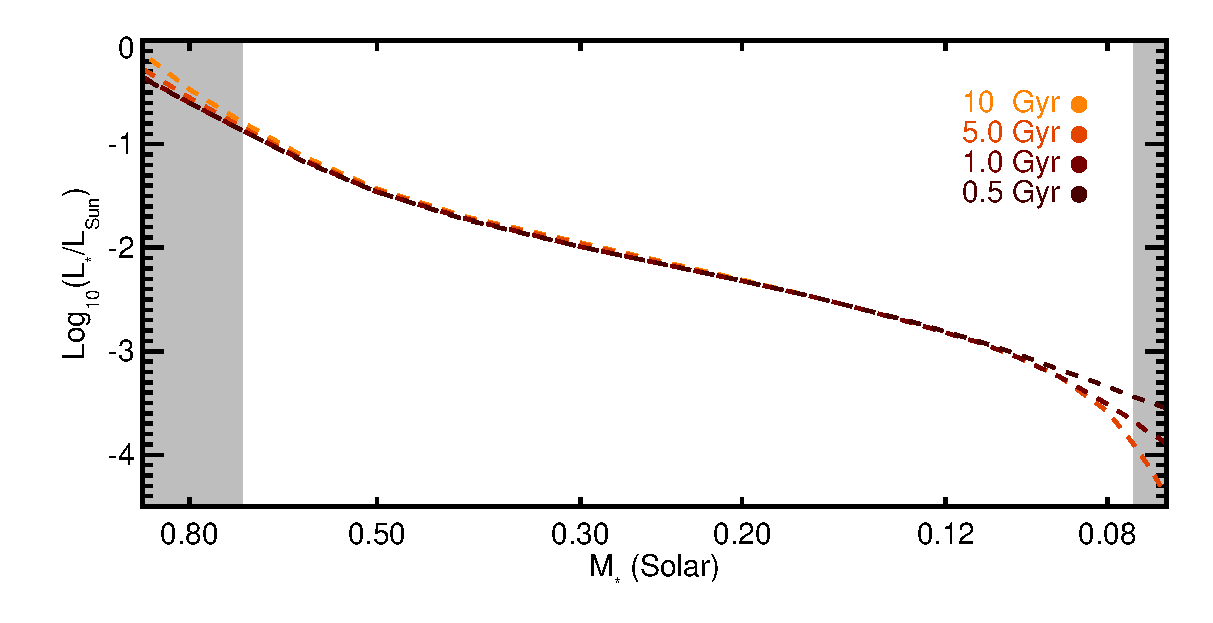
\includegraphics[width=0.47\textwidth]{Model_age2.eps}
\caption{Stellar luminosity as a function of mass predicted by the \citet{BHAC15} models, color-coded by age (metallicity fixed at Solar). The grey regions denote masses excluded by this study due to a significant age dependence on the mass-luminosity relation.}
\label{fig:age}
\end{center}
\end{figure}

We first selected systems by cross-matching catalogs of nearby M dwarfs \citep{Lepine:2013, Gaidos2014, 2014ApJ...784..156D,Winters2015}, with the fourth catalog of interferometric measurements of binary stars \citep[INT4,][]{Hartkopf:2001}, and adaptive optics (AO) images from the Keck Observatory Archive (KOA). As part of this cross-match, we also included targets matching the M dwarf selection criteria of \citet{Gaidos2014}, but with a bluer color cut ($V-J>1.8$) to incorporate additional late-K dwarfs. We kept any binaries with separations less than 5\arcsec. We then added in other known late-type binaries from \citet{2008MNRAS.384..150L}, \citet{Janson2012}, \citet{Jnn2014}, and \citet{Ward-Duong2015}. This provided a list of more than 300 multi-star systems.

From here we selected binaries for which we expect to be able to obtain a precise orbit on a reasonable (few year) timescale. We assumed that the average of available (literature) separation measurements approximate the semi-major axis of the system. We then identified systems for which we would have at least 30\% of the orbit, including the two years of our orbital monitoring program with Keck. This cut accounted for existing data. As a result, long-period binaries with extensive previous observations were included, depending on the baseline available, while those with only a single epoch would generally need to have orbits of $\ll$10 years to be observed. After this cut we were left with 125 systems. Excluding 38 systems at $\delta<-30~deg$ that are difficult to observe from Maunakea, 87 systems were included in our observing program.

We removed 21 systems from our analysis because of an unresolved tertiary (or quaternary) component noted in the literature \citep[e.g.,][]{2010ApJ...720.1727L,2002A&A...382..118T,2018ApJS..235....6T}. In their current form, such systems were not useful for our analysis, as we had no $\Delta K$ magnitudes or mass ratios for the unresolved components. Since many of these are double- or triple-lined systems, it is possible to recover their parameters with multi-epoch radial velocities, and some systems have the necessary data in the literature \citep[e.g.,][]{Sgr2000}. We continued to monitor these systems with high-resolution near-infrared spectrographs \citep{2010SPIE.7735E..1MY, 2012SPIE.8446E..2CR, Park2014}, but they were excluded from the analysis done here. High-order systems where all components are resolved (e.g., GJ 2005 ABC) are retained, although we only focus on the tighter pairs in this paper. 

A total of 18 systems were flagged as young, i.e. affiliated with nearby young moving groups or clusters \citep{Shkolnik2012, Kraus2014, Gagne2014, Malo2014a, Gagne2015, 2017AJ....153...95R, 2017AJ....154...69S, Rizzuto2017, 2018MNRAS.475.2955L}. We monitored these targets even after flagging them as young, but they were not included in the analysis for this paper. Many of these are likely pre-main-sequence stars and hence will not follow the same mass-luminosity relation. Even for those that are on the main-sequence, young M dwarfs may have higher luminosities for a given mass due to effects of activity and spots \citep[e.g.,][]{2015ApJ...807....3K,Stassun2012,Somers2017}. These young systems will be the subject of a future study into the effects of age and activity on the parameters of M dwarfs. We note that this cut did not remove any young stars in the field population.

After the completion of our observing program, we removed targets for which we had $<$30\% of the orbit or fewer than six independent measurements. We attempted to fit orbits of the remaining 75 systems (Section~\ref{sec:orbit}). Seven of the orbits fits failed to converge, mostly because their semi-major axes were much larger than expected (e.g., eccentric systems caught near periapsis). An additional 16 were removed because the derived mass for the system was too imprecise ($>$20\% errors on $M_{tot}$) to be useful. Most of these 16 were systems with a poor or no parallax measurement. This left us with 52 binaries (106 stars).

We added in seven targets with orbits from \citet{Dupuy2017}, primarily to fill in the sample around the end of the M dwarf sequence. These seven were selected because they are theoretically massive enough to sustain hydrogen fusion and satisfy all our other selection criteria. Systems from \citet{Dupuy2017} also had their orbits fit using a nearly identical method to our own, often using similar or identical sources of data and analysis methods (primarily Keck/NIRC2). Two addition systems in \citet{Dupuy2017} matched our initial cut, but were still omitted from this analysis. These were LP415-20, which \citet{Dupuy2017} argue is an unresolved triple, and 2M1847+55, which has a relatively imprecise orbit compared to the rest of the sample.

Parameters of the final 59 systems included in our analysis are given in Table~\ref{tab:sample}.

\section{Observations and Data Reduction}\label{sec:obs} 

\subsection{Near-infrared Spectra with IRTF/SpeX}

To estimate the metallicities of our targets we obtained near-infrared spectra for 56 of 59 targets using the SpeX spectrograph \citep{Rayner2003} on the NASA Infrared Telescope Facility (IRTF) atop Maunakea. Observations were taken between May 2011 and November 2017. Most data were taken as part of programs to characterize the fundamental properties of nearby M dwarfs \citep[e.g.,][]{Mann2013c,Gaidos2014,Terrien2015}. All spectra were taken in SXD mode, providing simultaneous wavelength coverage from 0.9 to 2.5$\mu$m. For 56 of the targets, observations were taking using the 0.3$\times15\arcsec$ slit, which yielded a resolution of $R\simeq2000$. Spectra for two targets were taken from \citet{2009ApJ...706..328D}, \citet{Dupuy2012}, or \citet{Dupuy2017}, using the 0.5$\times15\arcsec$ or 0.8$\times15\arcsec$ slits, which gave spectral resolutions of $\simeq$750-1500. 

For Gl 65 and HD 239960 the SpeX slit was aligned to get spectra of both targets simultaneously. For all other targets the binary was unresolved or too poorly resolved to separate in the reduction procedure, and instead the slit was aligned with the parallactic angle. Each target was nodded between two positions along the slit to remove  sky background. Depending on the target brightness and conditions, between 6 and 30 individual exposures were taken following this nodding pattern, with exposure times varying from 8s to 180s. An A0V-type star was observed immediately before or after each target to measure (and remove) telluric lines and flux calibrate the spectrum. The final stacked spectra had S/N of $>100$ per resolving element in the $K$-band for all but the four faintest targets (which had S/N$>50$). 

Basic data reduction was performed with {\tt SpeXTool} package \citep{Cushing2004}. This included flat fielding, sky subtraction, extraction of the one-dimensional spectrum, wavelength calibration, stacking of individual exposures, and merging of separate orders. Telluric lines were removed and the spectrum was flux calibrated using the A0V star observations and the \textit{xtellcor} software package \citep{Vacca2003}. When possible, the same A0V star was used for multiple targets taken near each other in time. 

Two of the three targets lacking SpeX spectra are too warm (earlier than K5) to derive a metallicity from NIR spectra (Gl 792.1 and Gl 765.2), and the third (Gl 54) is too far south to be observed with IRTF. 

\subsection{Adaptive Optics Imaging and Masking}\label{sec:ao}

We analyzed a mix of AO data from our own program with Keck/NIRC2 and archival imaging from the Keck II Telescope, the Canada France Hawaii Telescope (CFHT), the Very Large Telescope (VLT), and the Gemini North Telescope. In general we analyzed all usable images (e.g., non saturated, components resolved) regardless of observing mode and filter. 

For our analysis, we considered a single dataset a collection of observations with a unique combination of filter, target, and epoch. Each combined dataset consisted of a $\Delta m$ (for a given filter), separation, and position angle. 

We separate the observations and reduction by instrument/telescope below. The full list of astrometry and contrast measurements is given in Table~\ref{tab:astrom}, sorted by target and date. 

\subsubsection{Keck II/NIRC2 Imaging and Masking}

As part of a long-term monitoring program with Keck II atop Maunakea, between June 2015 and November 2017 we observed 49 of the 52 multiple-star systems fit in this paper. All observations were taken using the facility AO imager NIRC2 in the vertical angle mode (fixed angle relative to elevation axis) and the narrow camera ($\approx$10\,mas\,pixel$^{-1}$). Depending on target brightness and observing conditions, images were usually obtained through either the $K'$ ($\lambda_c=2.124$\um) or narrow $K_{\rm{cont}}$ ($\lambda_c=2.2706$\um) filters, and non-redundant aperture masking (NRM) was always taken using the 9-hole mask and $K'$ filter. After acquiring the target and allowing the AO loops to close, we took four to 10 images or 6-8 interferograms, adjusting coadds and integration time based on the brightness of the target. As most of our targets are bright, observations were usually taken using the Natural Guide Star (NGS) system \citep{2000PASP..112..315W,2004ApOpt..43.5458V}, only utilizing the Laser Guide Star (LGS) mode for the faintest ($R\gtrsim13$) targets or in poor conditions. In total, our observations provided 154 datasets.

In addition to our own data, we downloaded images from the Keck Observatory Archive (KOA), spanning March 2002 to November 2015, all of which were taken with the NIRC2 imager. Archival data comprised a wide range of observing modes, filters, and cameras, although the majority was taken with the narrow camera and either the $H$- or $K$-band filter. We included nearly all data with clear detections of both binary components independent of the observing setup. We discarded saturated images, those taken with the coronagraph for either of the component stars, and those with extremely poor AO correction. A total of 36 datasets were used from the archive. 

The same data reduction was applied to observations both from our own program and from the archive, following our custom procedure described in \citet{Kraus2016a}. To briefly summarize, we corrected for pixel value nonlinearity in each frame then dark- and flat-corrected it using calibrations taken the same night. In cases where no appropriate darks or flats were taken in the same night, we use a set from the nearest available night. We interpolated over ``dead'' and ``hot'' pixels, which were identified from superflats and superdarks built from data spanning 2006 to 2016. Because flats are rarely taken in narrowband filters, we used superflats built from the nearest (in wavelength) broadband filter where appropriate (e.g., for $K_{\rm{cont}}$ we used $K'$ flats). Pixels with flux levels $>10\sigma$ above the median of the eight adjacent pixels (primarily cosmic rays) were replaced with the median (average of the 4th and 5th ranked). Images were visually inspected as part of identifying the binary location, and a handful ($<$1\%) of images were negatively impacted by our cosmic ray removal (e.g., removal of part of the source). These images were manually corrected.


\subsubsection{CFHT/PUEO Imaging}

We obtained data for 31 of our targets from the Canadian Astronomy Data Centre archive, taken with the 3.6m Canada-France-Hawaii Telescope (CFHT) using the Adaptive Optics Bonnette \citep[AOB, often referred to as PUEO after the Hawaiian owl,][]{1994SPIE.2201..833A} and the KIR infrared camera \citep{1998SPIE.3354..760D}. After removing bad observations (e.g., saturated, unresolved, or poor AO correction), a total of 226 datasets were included. Observations spanned December 1997 to January 2007, covering most of the time PUEO was in use at CFHT (1996 to 2011). Most observations were taken in a few-year period from 2000 to 2003. Observations spanned a range of filters across $JHK$ bands, but the majority used either the narrowband [Br$\gamma$] or [FeII] filters. All observations used a 3-5 point dither pattern and took at least two images at each dither location. 

Data reduction for PUEO observations followed the same basic steps as our NIRC2 data. We first applied flat-fielding and dark correction using a set of superflats and superdarks built by splitting the datasets into 6 month blocks and combining calibration data within the same time period. We identified bad pixels by median filtering stacks of science images taken of dozens of objects, which were then replaced with the median of the eight surrounding pixels. To identify cosmic rays, we median-filtered consecutive images of each target (at a fixed location), then compared the stack to individual images. Pixels $>10\sigma$ above the robust mean of the stacks are replaced with the median of the eight surrounding points. Because PUEO/KIR data were taken in sets of $>$5 images before the object was dithered, this median-filtering was effective for removing nearly all cosmic rays.


\subsubsection{VLT/NaCo Imaging}

We downloaded AO-corrected images from the ESO archive taken with the Nasmyth Adaptive Optics System Near-Infrared Imager and Spectrograph (NAOS-CONICA, or NaCo) instrument on VLT. Data spanned November 2001 to October 2016, with about half of these 70 datasets taken from 2001 to 2005. Based on the program abstracts, $\lesssim$1/2 of the observations were meant to use these binaries as astrometric or photometric calibration (e.g., science case is unrelated to M dwarfs or binaries). Data covered 20 of our targets, excluding saturated or otherwise unusable data. Observations were taken with a wide range of filters, cameras, and observing patterns, but the majority were taken using the S13 camera ($\approx$13\,mas\,pixel$^{-1}$) with either broadband $K_s$ and $L$, or narrowband [FeII] and [Br$\gamma$] filters, and always following a 2-4 point dither pattern. 

Basic data reduction was applied to NaCo images following a similar procedure with the PUEO and NIRC2 data. We applied flat-fielding and dark corrections to each observation using the standard set of calibrations taken each night as part of the VLT queue. In the case where calibration (dark or flat) images were missing or unusable, we used the nearest (in time) set of calibration images matching the filter (for flats) and exposure setup (for darks). Flats taken in broadband filters were used for flat-fielding narrow-band images at similar wavelengths. We built bad pixel masks using median stacks of all images taken within a night after applying flat and dark corrections. To identify and remove cosmic rays we used the L.A. Cosmic software \citep{2001PASP..113.1420V}.


\subsubsection{Gemini/NIRI Imaging}

We retrieved 39 datasets for 8 of our targets from the Gemini archive, all taken with the AO imager NIRI \citep{2003PASP..115.1388H} on the Gemini North Telescope. All observations were taken between August 2008 and February 2011 and were taken with the assistance of the ALTtitude conjugate Adaptive optics for the InfraRed (ALTAIR). Most observations were taken with the f32 camera ($\approx$21\,mas\,pixel$^{-1}$) using broadband $J$-, $H$-, or $K$-band filters. All observations followed a 2-4 point dither pattern and took at least two images at each dither location. 

Data from NIRI were reduced using the same basic methods as for all other adaptive optics data. First, we applied flat and dark corrections to each set of images using the standard calibration images taken as part of the Gemini queue, usually within 24h of the target observations. In most cases, flats taken in broadband filters were used for narrowband flat-fielding. We then identified bad pixels from median filtering of all images within a given night. Observations with a target near or on top of a heavily impacted pixel (identified with the mask) were discarded. We used the L.A. Cosmic software for the identification and removal of cosmic rays. 

\section{Astrometry and photometry}\label{sec:astrometry}

Extracting separations and position angle measurements followed a similar multi-step procedure across all instruments, excluding the NRM data (which is described below). Our method is based largely on that described in \citet{2016ApJ...817...80D} and \citet{Dupuy2017}, which is built on the techniques from \citet{2008ApJ...689..436L} and \citet{2010ApJ...721.1725D} and we briefly describe here. 

We first cross-correlated each image with a model Gaussian PSF to identify the most significant peaks. The cross-correlation peak occasionally centers on instrumental artifacts, often struggles to separate out partially overlapping binaries, and can easily identify the wrong source for triple systems. So this step was checked by eye and updated as needed. The eye-check phase also allowed us to manually remove data of poor quality: e.g., no or poor AO correction, saturated data, or an unresolved system. We used these centers as the initial guess for the $x, y$ pixel position used in the next phase. 

We then fit the PSF centers by either: 1) fitting the binary image with a PSF modeled by three-component elliptical 2D Gaussians using the least-squares minimization routine MPFIT \citep{Markwart2009}, or 2) running {\tt StarFinder}, a routine designed to measure astrometry and photometry from adaptive optics data by deriving a PSF template from the image and iteratively fitting this model to the components \citep[for more details, see][]{2000A&AS..147..335D}. Although the results of these two methods generally agreed, {\tt StarFinder} was preferred, as it used a non-parametric and more realistic model of the PSF and worked even with mediocre AO correction, provided the component PSFs were well separated. {\tt StarFinder}, however, failed on the tightest binaries, where it was unable to distinguish two stars and thus incorrectly built a pathological, extended PSF that fit the blended image. The Gaussian fit was used for these cases where {\tt StarFinder} failed. 

As part of the PSF fit, both methods provide a flux ratio of the PSF normalization factors, which we used this to determine the contrast $\Delta m$ in the relevant band. Data from all filters are used for astrometry, although only $\Delta K$ measurements were used in the estimate of \mks\ (see Section~\ref{sec:mags}).

PSF fitting provides pixel-position ($x$, $y$) measurements of each component, but converting these to separation ($\rho$) and position angle (PA) on the sky requires an astrometric calibration of the instrument. For the NIRC2 narrow camera, we used the \citet{Yelda2010} distortion solution for data taken before 2015 Apr 13 UT, and \citet{2016PASP..128i5004S} for data taken after this. These calibrations include a pixel scale and orientation determination of 9.952$\pm$0.002 mas\,pixel$^{-1}$ and $0.252\pm0.009\,deg$ for the former, and 9.971$\pm$0.004 mas\,pixel$^{-1}$ and $0.262\pm0.020\,deg$ for the latter. For the NIRC2 wide camera we used the solution from Fu et al. (2012, priv. comm.)\footnote{\href{http://homepage.physics.uiowa.edu/~haifu/idl/nirc2wide/}{http://homepage.physics.uiowa.edu/$\sim$haifu/idl/nirc2wide/}}, with a pixel scale of $39.686\pm0.008$ mas\,pixel$^{-1}$ and the same orientation as the narrow camera. For the f/32 camera on NIRI, we used the distortion solution from the Gemini webpage\footnote{\href{http://www.gemini.edu/sciops/instruments/niri/undistort.pro}{http://www.gemini.edu/sciops/instruments/niri/undistort.pro}}. 

For other instruments and cameras, data were always taken following a dither pattern to sample different regions of the CCD distortion pattern. So the RMS between dithered images should reflect errors due to uncorrected distortion (which is included in our errors; see below). For KIR, we adopted a pixel scale of 34.8$\pm$0.1 mas pixel$^{-1}$ \citep{2003ApJ...589..410S} and an orientation of $0\pm2$~deg\footnote{\href{http://www.cfht.hawaii.edu/Instruments/Detectors/IR/KIR/}{KIR specifications, filters, and performance.}}. For NaCo, we assumed a pixel scale of 13.24$\pm0.05$ mas pixel$^{-1}$ for the S13 camera \citep{2003A&A...411..157M,2005A&A...435L..13N} and the values given in the ESO documentation for all others\footnote{\href{http://www.eso.org/sci/facilities/paranal/instruments/naco/doc.html}{NaCo Documentation, user manual, calibration, and reduction.}} (with the same error). The rotation taken from the NaCo headers was assumed to be correct to 0.4~deg. \citep{Sef2008}. For NIRI observations, we used a pixel scale provided in the Gemini documentation\footnote{\href{http://www.gemini.edu/sciops/instruments/niri/imaging/pixel-scales-fov-and-field-orientation}{NIRI pixel scales, field of view, and field orientation.}} for each camera (117.1, 49.9, and 21.9 mas pixel$^{-1}$ for f/6, f/14, and f/32, respectively), with a global uncertainty of 0.05 mas pixel$^{-1}$ on the pixel scale and 0.7~deg. on the orientation. The NIRI orientation error was determined using observations of the same target between observing runs (separated by weeks to months), but over which no orbital motion should have been visible ($P\gg50$ years). 

Calculation of separations and position angles from of non-redundant masking (NRM) observations followed the procedures in the appendix of \citet{Kraus2008} with the aid of the latest version of the ``Sydney'' aperture-masking interferometry code\footnote{\href{https://github.com/mikeireland/idlnrm}{https://github.com/mikeireland/idlnrm}}. To remove systematics, each NRM observation of a science star was paired with that of a single calibrator star taken in the same night with a similar magnitude and airmass. Binary system profiles were then fit to the closure phases to produce estimates of the separation, position angle, and contrast of the binary components. More details on the analysis of masking data can be found in \citet{2006ApJ...650L.131L}, \citet{Kraus2008} and \citet{2012ApJ...744..120E}.

All data in a single set (same target, filter, and night) were combined into a single measurement (after applying all corrections above), with errors estimated using the RMS in the individual images within a night. This scatter across images was combined with the uncertainty in the orientation and pixel scale in quadrature. We assumed that the pixel scale and orientation uncertainties were completely correlated within a night and filter so they do not decrease with $\sqrt{N}$. 

We also corrected separation and position angle for differential atmospheric refraction \citep{2010SPIE.7736E..1IL} using filter wavelength information and weather data from the header (for VLT) or from the CFHT weather archive\footnote{\href{http://mkwc.ifa.hawaii.edu/archive/wx/cfht/}{CFHT weather archive.}} (for Keck, CFHT, and Gemini). We neglected the chromatic component of this effect as the correction is already small compared to measurement errors. 


\subsection{Literature Astrometry}\label{sec:litas}

We included  measurements from the literature for 50 of the 52 binaries in our sample for which we analyzed astrometry. To help identify sources of astrometry, we used the fourth catalog of interferometric observations of binary stars \citep[INT4,][]{Hartkopf:2001}. We only used measurements that included both a separation and position angle. In cases where the literature data was also available in one of the archives above (i.e., the same dataset used in the reference), we adopted our own measurements over the literature data to ensure more homogeneous measurements and errors. We did not utilize $\Delta m$ measurements from the literature, although in some cases this information was used to verify the astrometry was for the correct binary system or component.  

In total, we used 558 measurements (each including a separation and position angle) from 60 references. The literature astrometry was very non-uniform; roughly half of the points were for just 11 targets, predominately taken with the goal of measuring their orbits. Approximately 180 measurements came from speckle observations on the Special Astrophysical Observatory (SAO) 6m \citep[e.g.,][]{Bag2002}, WIYN \citep[e.g.,][]{Hor2017}, or SOAR \citep[][]{Tok2017b} telescopes. About 160 points came from {\it HST}, primarily Fine Guidance Sensors measurements  of $\sim$10 binaries \citep[e.g.,][]{Benedict2016}. The rest of the measurements are from a mix of surveys focusing on taking many epochs of specific systems to determine orbits \citep[e.g.,][]{Koh2012} and broader surveys (e.g., for multiplicity) that obtain 1-2 epochs on each of dozens of binaries \citep[e.g.,][]{Janson2012}.  

One complication using older literature astrometry is inhomogeneous reporting of separation and position angle errors. Many references provided measurements without errors, and many more reported errors without accounting for field distortion or errors in the pixel scale and orientation. We mitigated this problem by generating an error common to a given reference. For each literature source, we identified a set of binaries where an orbit can be fit (with $<$5\% errors on the angular separation) without astrometry from that particular reference. Some literature sources were merged for this comparison, provided they used the same instrument and basic analysis. We included binaries outside the sample considered here. We fit the orbit following the method outlined in Section~\ref{sec:orbit}, using only the least-squares method for efficiency. We then compared the expected position angle and separation to the measurements from the reference in question. From this difference we computed the required missing error term, which, when added in quadrature with the reported errors (zero for those without errors) would yield a reduced $\chi^2$ ($\chi^2_\nu$) of 1. References where we could not test the reported errors (e.g., due to insufficient data) and those with extremely large aded error terms ($>$50\,mas) were not used. No reference gave a negative term (over-reported errors). The final term was added in quadrature with literature reported uncertainties (if any were reported). 

%As a test, we repeated this test on AO data analyzed in this paper, attempting to derive a missing error term. In all cases the resulting error term was negligibly small compared to other errors, and for CFHT/PUEO value was slightly negative (but still smaller in magnitude than other uncertainties). As a result we did not apply any term to data we analyzed. 

All literature astrometry used in this paper is listed alongside our own measurements in Table~\ref{tab:astrom}. 

\subsection{Summary of input astrometry}

In total we measured or gathered 1083 unique datasets (unique filter/night/target combinations), approximately half of which we measured from adaptive optics images (525) and the other half were drawn from the literature (558). Most of the astrometry measurements derived from our analysis came from either NIRC2 (190) or PUEO (226), with a smaller contribution from NaCo (70) and NIRI (39). 

Although they represent only $\simeq$20\% of the total astrometric measurements, the NIRC2 measurements are the most critical in constraining orbital parameters. NIRC2 astrometry was 1-2 orders of magnitude more precise than those from the literature, and a factor of 3-8$\times$ more precise than those from PUEO, NIRI, and NaCo. We characterized the relative importance of each data source using the total number of unique separation measurements weighted by their uncertainties (1/$\sigma$). Under this metric, the NIRC2 points contributed $\gtrsim10\times$ more orbital information than the literature data. Measurements from CFHT/PUEO had a comparable total contribution to the literature data, each of which had $\simeq2\times$ the impact of NaCo measurements, and $\simeq3\times$ that of data from NIRI. This comparison likely underestimated the importance of the NIRC2 data; literature and archive images tended to be concentrated on the best-characterized systems, while our NIRC2 observations were specifically coordinated to complete orbits and cover under- or un-sampled regions of binary orbits. However, the combination of NIRC2 and literature and/or PUEO points is the most useful, since this provides both the precision and long baseline (PUEO and NIRC2 data is typically separated by $>15$\,years) needed to fully constrain the orbital parameters.

\section{Orbit Fitting}\label{sec:orbit}

We fit the astrometry with the Monte Carlo Markov Chain (MCMC) software {\tt emcee} \citep{Foreman-Mackey2013}, a Python implementation of the affine-invariant ensemble sampler \citep{goodman2010}. For each system, we explored seven orbital elements: the orbital period ($P$), combined angular semi-major axis ($a\arcsec$), eccentricity ($e$), inclination ($i$), epoch of periastron passage ($T_0$), argument of periastron ($\omega$), and position angle of the line of nodes ($\Omega$). Parameters were limited by physical or definitional constraints, e.g., $P>0$, $0<e<1$, and $0<i<\pi$, but were given no additional boundaries. 

We applied non-uniform priors of 1/$P$, 1/$a\arcsec$, and $\sin(i)$ to $P$, $a\arcsec$, and $i$, respectively. All other parameters evolved under uniform priors. Walkers were initialized with the best-fit orbit determined using \textit{MPFIT} \citep{Markwart2009} and a spread in starting values based on the \textit{MPFIT} estimated errors. Each MCMC chain was initially run for $10^5$ steps with 100 walkers. We tested to see if a chain converged using the autocorrelation time \citep{2010CAMCS...5...65G} and chains were checked by eye for signs on convergence. In about 1/4 of the systems the fit did not converge after the initial $10^5$ steps, so we ran these for $10^6$ total steps. Those that did not converge after $10^6$ steps were not included in our final sample. These were not included in our final sample of 59 binaries (see Section~\ref{sec:targets}), as these were the least-well characterized systems. We saved every 100 steps in the chain, and the first 5\% of each chain was removed for burn-in. 

Systems of near-equal mass may have the primary and companion confused, both in our own measurements and also those taken from the literature. We identified such measurements by eye during the \textit{MPFIT} stage and manually adjusted the position angles before starting the MCMC run. In total $\simeq$16 measurements were corrected this way, almost all of which were for three systems with contrast ratios close to unity. A more robust solution to this problem would be to feed a double-peaked prior at the reported value and $\pm$180~deg. into the likelihood function. However, in all cases the problematic points were obvious by eye, had reported $\Delta m$ consistent with zero, and a simple 180~deg correction completely fixed the orbit. 


\begin{figure*}[htb]
\begin{center}
\includegraphics[width=0.32\textwidth]{Orbits/Gl301BAB.eps}
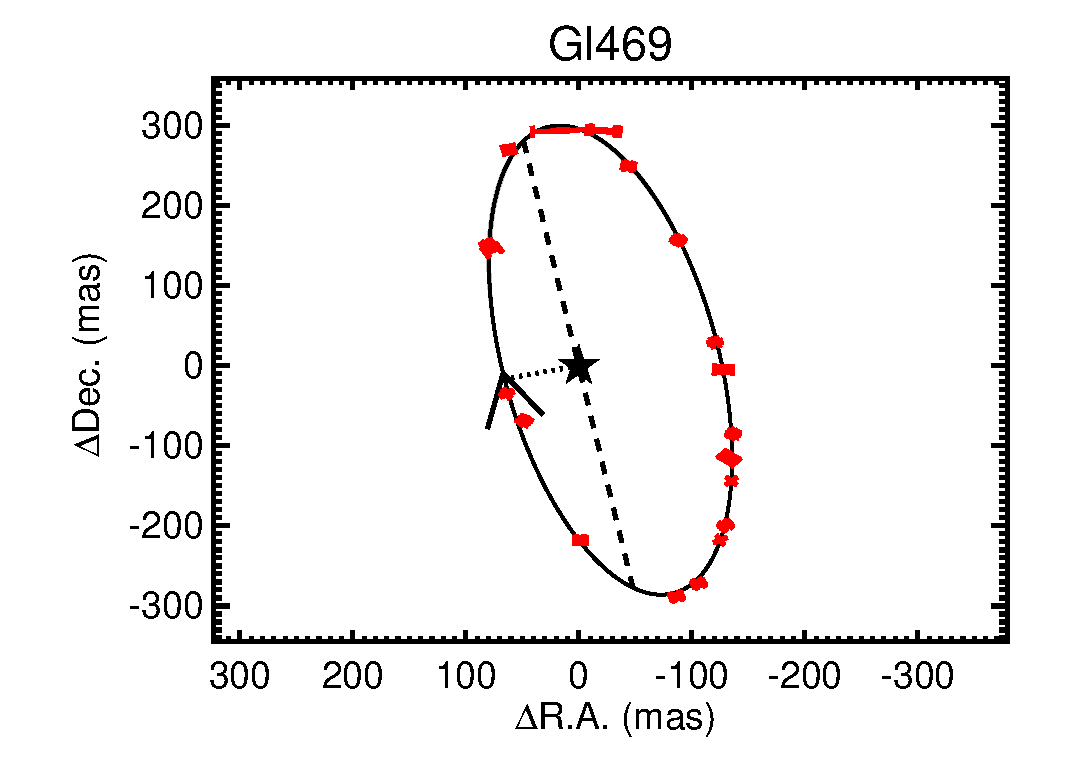
\includegraphics[width=0.32\textwidth]{Orbits/Gl469AB.eps}
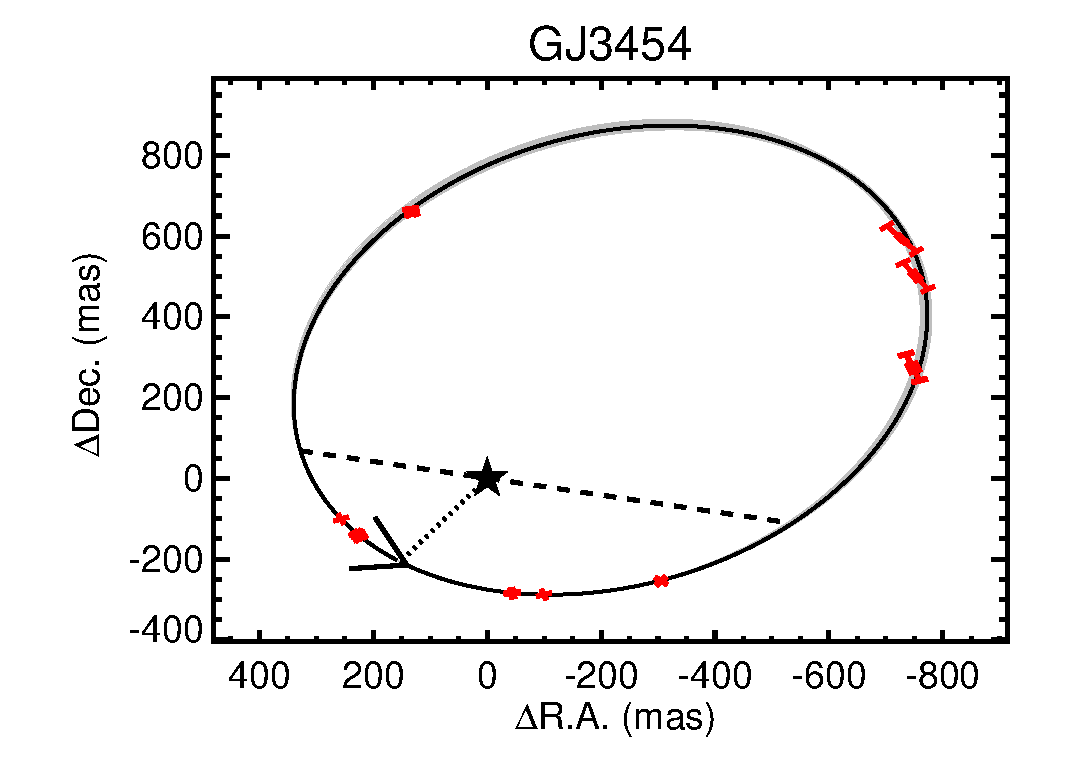
\includegraphics[width=0.32\textwidth]{Orbits/GJ3454AB.eps}
\caption{Example results of our orbit fitting procedure for Gl 301AB (left), Gl 469AB (middle), and GJ 3454AB (right). Points are individual measurements of the separation and position angle, color-coded by the astrometry source. Black solid line shows the best-fit (highest likelihood). Dark grey lines are drawn by randomly sampling 50 orbit fits from the MCMC chain to display an estimate of the errors. The dotted line connects periastron passage, with an arrow pointing in the orbital direction, and the dashed-line showing the line of nodes. For Gl469AB, high-quality astrometry is available for the full orbit, and the resulting errors on orbital parameters are so small that the grey lines cannot be seen. All orbits are shown in Appendix~\ref{sec:a1}.}
\label{fig:orbits}
\end{center}
\end{figure*}

Overall the quality of the fits is extremely good, with $\chi^2_\nu$ values ranging from 0.1 to 2, and cumulative distribution values (the probability of getting the $\chi^2$ or smaller given the degrees of freedom) ranging from 2\% to 99\% (mean probability of 47\%). We show some example orbital fits in Figure~\ref{fig:orbits} (with the full set in Appendix~\ref{sec:orbitplots}) and provide the median orbital parameters in Table~\ref{tab:orbits}. Orbits span a wide range in period; the tightest binaries have $P<1$\,yr, while the widest have $P>50$\,yr. The two systems with $P>50$\,yr (Gl 301 and Gl 277) were also some of the least-well characterized. No systems show evidence of period-doubling due to limited sampling, an advantage of using data with non-uniform temporal sampling.

Our orbital fits made heavy use of literature astrometry, many of which had no reported errors. Our method for assigning or correcting errors assumed that all measurements have a common missing error term per source (Section~\ref{sec:litas}). It is more likely that errors depend on the separation and contrast ratio, as well as quantities that were not consistently reported, like weather, setup, and observational strategy. Further, this technique assumed an uncorrelated error term. In the case of an erroneous pixel scale or imperfectly aligned instrument, all measurements from a common instrument err in the same sense.   In practice, it is difficult to correct for these effects without access to the actual images. The data suggest this does not impact our results; the final $\chi^2_\nu$ values for the best-fit orbits shows no correlation with the fraction of astrometry from the literature versus our own measurements, and measurements taken on the same target and night but from different sources agree within errors. 

As an additional test, we tried refitting six binaries with the most literature data twice, first doubling the error term added to the literature points, then halving it. In all cases, overall parameters and errors did not change significantly (although the final $\chi^2_\nu$ values changed). The main reason for this is that our new measurements are generally far more more precise (with the exception of measurements from {\it HST}) and hence dictate the final solution, even in cases where most of the individual measurements are from the literature. In the case of halving errors, the MCMC landed on a similar solution, but with smaller parameter uncertainties and increased $\chi^2$ values. We conclude this treatment of errors does not significantly impact our final orbital fits and that our assigned errors are reasonable overall.

\section{Stellar Parameters}\label{sec:params}

\subsection{Parallaxes}\label{sec:plx}

Parallaxes for 56 of the 59 systems were drawn from the literature. In general we adopted the most precise parallax available, although preference was given to those accounting for centroid motion of the binary and those with a baseline significantly different from the binary's orbital period. A few systems are in hierarchical triples with a wider companion that has a separate (mostly independent) parallax measurement, which we used where possible. For $\simeq$1/3 of the sample, we drew parallaxes from the new reduction of the Hipparcos data \citep{van-Leeuwen:2007yq}. For the seven systems in \citet{Dupuy2017}, we used their parallaxes, and those from \citet{Benedict2016} for 13 systems in both samples. For nine systems we pulled parallaxes from the general catalogue of trigonometric parallaxes \citep{van-Altena1995}. 

About half (28) of our targets do not have entries in the second data release of Gaia \citep[DR2, ][]{GaiaDr2,2018arXiv180409365G}. They were likely excluded because centroid shifts from orbital motion prevented a five-parameter (single-star) solution (a requirement to be included in DR2). We also found significant differences between the Gaia DR2 values and earlier measurements \citep[including from Gaia DR1, ][]{gaiadr1} even when measurements were available. Many wide triples in Gaia DR2 (where the third star is several arc seconds away, and hence easily resolved) have significantly different parallaxes reported for the unresolved pair than for the wider companion. Orbital motion is likely impacting the parallax values or uncertainties, an issue that should be resolved in future Gaia data releases that will include fits for orbital motion. We found no such issues with our other parallax sources. So we decided to not use Gaia DR2 parallaxes in most cases. 

We ultimately adopted Gaia DR2 parallaxes for three systems, GJ1245AC, GJ277AC, and GJ4287AB, where we adopted the parallax of their wider common proper motion companion. In all cases the wider associated stars are not known to harbor another unresolved star, and hence they should not be impacted by the same binarity issue. GJ 570BC, Gl 695BC, GJ 2005BC, Gl 22AC, and 2M1047+40 also have nearby associated stars. However, Gl 570A is extremely bright ($G\simeq5$) and hence may have an unreliable parallax due to saturation in DR2, GJ 2005A has no entries in Gaia DR2, the available parallaxes (from {\it HST} and Hipparcos) for Gl 695BC and Gl 22AC are similar or more precise than the those reported for Gl 695A and Gl 22B from Gaia DR2, and the wide pair to 2M1047+40 is itself a tight binary \citep[LP 213-67AB,][]{Dupuy2017} with a large reported excess astrometric noise in Gaia \citep[a sign of binarity,][]{2018RNAAS...2...20E}.

For three systems we derived new parallaxes using MEarth astrometry \citep{Nutzman:2008gf}. Updated parallaxes were measured following the procedure from \citet{2014ApJ...784..156D}. The only difference was we used a dataset with a baseline $\simeq$two years longer, which helps average out systematic errors arising from centroid motion due to the binary orbit, and significantly reduces the overall uncertainties. 

We list all parallaxes and references in Table~\ref{tab:sample}.

\subsection{Metallicity}\label{sec:feh}

We estimated [Fe/H] using our SpeX spectra and the empirical relations from \citet{Mann2013a} for K5-M6 dwarfs, and \citet{Mann2014} for M6-M9 dwarfs. These relations use a series of atomic lines (primarily Na, Ca, and K features) in the optical or NIR \citep[e.g.,][]{2010ApJ...720L.113R,Terrien:2012lr}, empirically calibrated using wide binaries containing a solar-type primary and an M-dwarf companion \citep[e.g.,][]{2005A&A...442..635B,Johnson2009,Neves2012}. The calibrations were based on the assumption that components of such binaries have similar or identical metallicities \citep[e.g.,][]{2015ApJ...801L..10T}. Similar methods have been used extensively to assign metallicities across the M dwarf sequence \citep[e.g.,][]{Terrien2015,Muirhead2015,Dressing2017,2018ApJ...853...30V,2018ApJ...854..145M}. Final adopted [Fe/H] values are given in Table~\ref{tab:sample}. Errors account for Poisson noise in the spectrum, but because of the relatively high SNR of the spectra, final errors on [Fe/H] are generally dominated by the uncertainties in the calibration itself, conservatively estimated to be 0.08~dex \citep{Mann2013a,Mann2014}.

For all but two systems (Gl 65 and HD 239960), our NIR spectra are for the combined flux of the binary components. \citet{Mann2014} explored the issue of measuring metallicities of binaries with unresolved data by combining spectra of single-stars with equal metallicities and re-applying the same calibration. The bias introduced is negligible ($\lesssim0.02$~dex) when compared to overall uncertainties. The added scatter is smaller than the measurement uncertainties, and can be almost entirely explained by the Poisson noise introduced in the addition of component spectra. This may be more complicated for nearly or marginally resolved systems, where the narrow slit (0.3\arcsec) is preferentially including light from one star. However, repeating the tests of \citet{Mann2014} and adding a random flux weighting to the fainter star produced a small change to the increased uncertainties (0.01-0.03\,dex).

Three systems (LP415-20, 2M2140+16, and 2M2206-20) have SpeX spectra taken with a wider slit, yielding lower spectral resolution. The bands in \citet{Mann2014} are defined using a homogeneous dataset taken with the narrow (0.3\arcsec) slit, so this difference may impact the derived [Fe/H]. We tested this by convolving a set of single-star SpeX spectra taken with the 0.3\arcsec\ slit with a Gaussian to put them at the appropriate lower resolution. The median of the derived [Fe/H] values changed by $<0.01$~dex, but the change varies between targets. Based on the resulting scatter, we estimate the errors on [Fe/H] from the lower-resolution spectra to be 0.12~dex on a Solar scale and 0.08~dex on a relative scale. These systems are marked separately in Table~\ref{tab:sample}. 

Two of the systems in our sample are L dwarfs (2M0746+20 and 2M1017+13). These are most likely above the hydrogen burning limit, and hence are included in our analysis. However, the \citet{Mann2014} method contains no L dwarf calibrators. Our derived [Fe/H] were extrapolations of the \citet{Mann2014} calibration. The \citet{Mann2014} calibration has only a weak dependence on spectral type, but we still advise treating the assigned values with skepticism until an L dwarf calibration becomes available. 

Two targets (Gl 792.1 and Gl 765.2) are too warm (earlier than K5) for the calibration of \citet{Mann2013a}. For these we take [Fe/H] values from \citet{2011A&A...530A.138C} and \citet{2010A&ARv..18...67T}, respectively. These [Fe/H] measurements are not necessarily on the same scale as those from \citet{Mann2013a}, which are calibrated against abundances of Sun-like stars from \citet{2015ApJ...805..126B,2016ApJS..225...32B}. Given reported variations in [Fe/H] for these stars, as well as [Fe/H] determination differences \citep{2014AJ....148...54H,2016ApJS..226....4H} we adopt conservative 0.08~dex uncertainties on both systems. For the other target lacking a SpeX spectrum (Gl 54), we derive [Fe/H] using the optical calibration of \citet{Mann2013a} and a moderate-resolution optical spectrum taken from \citet{Gaidos2014}.

\subsection{$K_S$-magnitudes} \label{sec:mags}

To determine $K_S$ magnitudes for each component we required both unresolved (total) $K_S$ for each system and the contrast ($\Delta K_S$) for each component. We adopted unresolved $K_S$ magnitudes from the Two Micron All Sky Survey \citep[2MASS,][]{Skrutskie2006}. Some of the brightest stars in our sample are near or beyond saturation in 2MASS. For these targets we recalculated $K_S$ magnitudes using available optical and NIR spectra, following the method of \citet{Mann2015a} and \citet{Mann2015b}, using available optical spectra from \citet{Gaidos2014}. Synthetic magnitudes were broadly consistent (mean difference of 0.003$\pm$0.002\,mag) with 2MASS $K_S$ magnitudes (and at similar precision) for fainter targets ($K_S>7$). We only updated $K_S$ magnitudes for bright systems where where our synthetic photometry differed from the 2MASS value by more than 2$\sigma$ (five systems). We mark these systems in Table~\ref{tab:sample}. 

Reddening and extinction are expected to be $\simeq$0 for all targets, as the most distant system is at 35\,pc, while the Local Bubble (a region of near-zero extinction) extends to $\simeq$70\,pc \citep{2009MNRAS.397.1286A}. So we did not apply any extinction correction to the adopted $K_S$ values.

To compute $\Delta K_S$, we used component contrast measurements from our adaptive optics data (Section~\ref{sec:astrometry}). While all targets considered here had at least one measurement in a filter centered with the $K$ band, none of the response functions used was a close match to 2MASS $K_S$. Many of the observations were taken with narrow-band $K_{\rm{cont}}$ ($\lambda_c\simeq2.27$\um) or Br$\gamma$ ($\lambda_c\simeq2.17$\um) filters (to avoid saturation), for example. We transformed these into 2MASS magnitudes before computing the final $\Delta K_S$. These corrections were usually small ($\lesssim0.1$ magnitudes), and details on their derivation are given in Appendix~\ref{sec:a1}.

After converting all contrast measurements to $\Delta K_S$, we combed multiple measurements using the robust weighted mean. Errors on contrasts for each dataset were taken to be the RMS in flux measurements among consecutive images. These errors may be underestimated because of imperfect PSF modeling, flat-fielding, uncorrected non-linearities in the detector, as well as intrinsic variability of the star. To test for this, we compared $\Delta K_X$ measurements of the same star using the same filter and instrument but on different nights (Figure~\ref{fig:magnitudes}). The comparison suggested a missing error term of 0.016\,magnitudes for NIRC2, 0.02 for PUEO and NaCo, and 0.03 for NIRI. We only tested this for $K$-band filters, but we found consistent values for different $K$-band filters from the same instrument. We included this term as an additional error term common to all measurements in our computation of $\Delta K_S$.

\begin{figure}[htb]
\begin{center}
\includegraphics[width=0.47\textwidth]{errors.eps}
\caption{Distribution of contrast ratio differences (in units of standard deviations) for data taken on the same target, and with the same filter and instrument, but in different nights. The red line is before adding the missing error term, while the blue line shows the distribution after adding this. The grey dashed line shows the expected Normal distribution. The histograms are offset slightly for clarity, although identical bins are used as input.}
\label{fig:magnitudes}
\end{center}
\end{figure}

%We did not use literature contrast ratios (even those in $K$-band), as we cannot perform and the same corrections applied to those from our own analysis. The exception was Gl 762.1, for which we have no AO data. For this target we adopt the value from \citet{CIA2010}.

For GJ 2005BC and Gl 900BC, the 2MASS PSF includes flux from the A component. In both cases we use our AO data to measure $\Delta K$ between all three components. The total $K_S$ magnitude given in Table~\ref{tab:sample} already have the A component removed. 

\section{The Mass-Luminosity Relation}\label{sec:relation}

\subsection{Methodology}

For main-sequence stars, the mass-luminosity relation traditionally takes the form:
\begin{equation}\label{eqn:ml}
\frac{L_*}{L_\odot} = C \left(\frac{M_*}{M_\odot}\right)^\alpha,
\end{equation}
where $\alpha$ depends on the dominant energy transport mechanism (e.g., radiative versus convective) and internal structure of the star \citep{2004sipp.book.....H}. 

We rewrite Equation~\ref{eqn:ml} in terms of \mks\ (and $\log(M_*/M_\odot)$) instead of $L_*$. Absolute magnitudes are more easily measured than overall luminosity, and avoid introducing errors from uncertain bolometric corrections or the need to take flux-calibrated spectra in order to measure the bolometric flux directly. Switching to \mks\ also mitigates effects of abundances. The $K$-band is heavily dominated by metal-insensitive CO and H$_2$O absorption bands. Optical bands are dominated by strong molecular (e.g. TiO, CO, CaH, MgH, and VO) bands that introduce a strong dependence on [Fe/H] and [$\alpha$/Fe] (Figure~\ref{fig:metal}). 

\begin{figure*}[htb]
\begin{center}
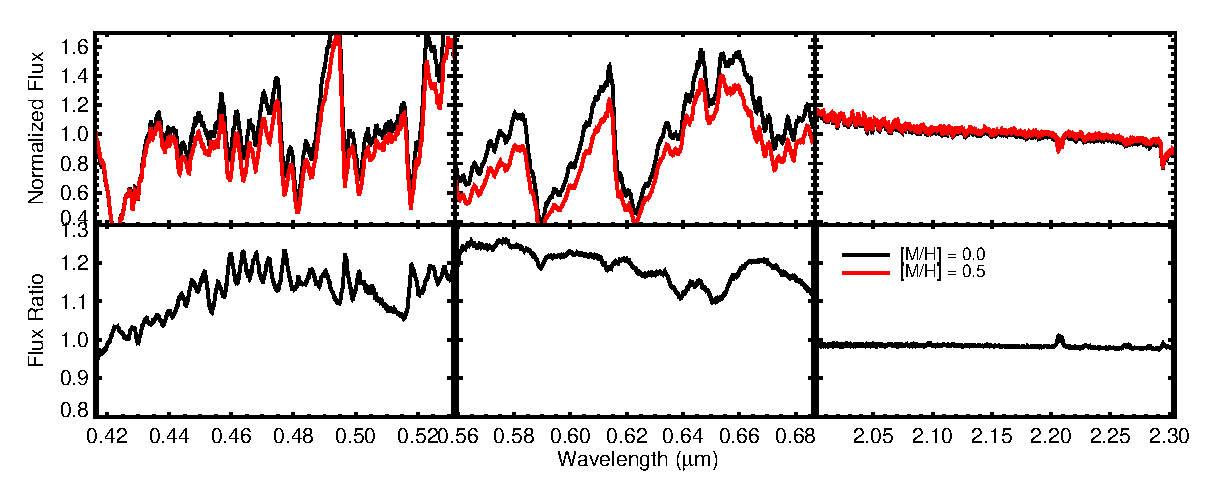
\includegraphics[width=\textwidth]{metallicity_effect.eps}
\caption{Effect of changes in [M/H] on a model spectrum at \teff=3200\,K, $\log(g)=5$ in $g$- (left), $r$ (middle), and $K$-band (right). The top panel shows [M/H]=0 (black) and [M/H]=+0.5 (red) spectra from the CFIST BT-SETTL models \citep{2012RSPTA.370.2765A}. The bottom panel shows the ratio of the two, highlighting how small an effect [M/H] has in the $K$-band compared to optical regions. The one feature that stands out in the $K$-band is the Na doublet, which is a commonly used as a metallicity diagnostic for dwarfs \citep{2010ApJ...720L.113R,Terrien:2012lr,Newton:2014}, and a gravity diagnostic for pre-main-sequence stars \citep[e.g.,][]{Schlieder2012}. }
\label{fig:metal}
\end{center}
\end{figure*}

Our sample encompasses almost an order of magnitude in mass and hence a range of underlying stellar physics. No single power law is expected to fit over the full sequence. Instead, we assumed that $\alpha$ depends on \mks, which we approximated as a polynomial. This yields a \mmk\ relation of the form:
\begin{equation}\label{eqn:mmk}
\log \left( \frac{M_*}{M_\odot} \right) = \sum_{i=0}^{n} a_i(M_{K_S}-zp)^i,
\end{equation}
where $a_i$ are the fit coefficients. The order of the fit ($n$) is determined using the Akaike Information Criterion \citep[AIC, ][]{Akaike1974}. The constant $zp$ is a zero-point (or anchor) magnitude, which we fixed at 7.5. This approximately corresponded to the logarithmic average mass of stars in our sample. 

For the left hand side, we computed the total system mass ($M_{\rm{tot}}$) for each binary by combining the the orbital period ($P$) and total angular semi-major axis ($a\arcsec$) from our fits to the orbital parameters (Section~\ref{sec:orbit}) with the parallaxes ($\pi$, Section~\ref{sec:plx}), following a rewritten form of Kepler's laws:
\begin{equation}\label{eqn:mass}
M_{\rm{tot}} = M_{1}+M_{2} = \frac{(a\arcsec/\pi)^3}{P^2},
\end{equation}
where $P$ is in years, $a\arcsec$ and $\pi$ are in arcseconds, and $M_{\rm{tot}}$ is in Solar masses. 

Because Equation~\ref{eqn:mass} does not provide component masses, when fitting for the $a_i$ coefficients we performed the comparison between the predicted and dynamical {\it total} mass for each system. For this, we rewrote Equation~\ref{eqn:mmk} in terms of total mass:
\begin{eqnarray}\label{eqn:mmk2}
M_{tot} &=& 10^{b_1} + 10^{b_2},\\
b_j &=& \sum_{i=0}^{n} a_i(M_{K_S,j}-zp)^i, \label{eqn:mmk2_b}
\end{eqnarray}
where \mks$_{,1}$ and \mks$_{,2}$ are the primary and companion absolute $K$-band magnitudes, which were calculated from our measured $\Delta K_S$ and unresolved $K_S$ magnitudes (Section~\ref{sec:mags}). Equation~\ref{eqn:mmk2} could easily be modified for higher-order star systems, providing individual \mks\ magnitudes and the total mass of the system are known. 

We fit for the $a_i$ terms in Equation~\ref{eqn:mmk2} using the MCMC code {\tt emcee}, which accounts for the strong covariance between coefficients. Each coefficient was allowed to evolve under uniform priors without limits, and was initialized with the best-fit value derived from \textit{MPFIT}. We ran the MCMC chain with 600 walkers for $10^6$ steps after a burn-in of 50,000 steps. We ran separate MCMC chains testing values of $n$ (fit order) from three to seven. 

Errors on the dynamical mass are correlated to the errors on \mks. The system mass scales with the cube of the semi-major axis, which depends linearly with the parallax. As a result, the parallax was a major, if not the largest, source of uncertainty on the mass for most systems. Similarly, our $K_S$ magnitudes had relatively small errors (0.01-0.03\,mag), so \mks\ errors tended to be dominated by the parallax. Because this correlation is usually along (parallel to) the direction of the \mmk\ relation, it can tighten the fit if properly taken into account (when compared to assuming uncorrelated errors). 

We wanted the MCMC to explore the full `ellipse' representing the correlation between \mks\ and $M_*$ for each binary. To this end, we treated the distance of each system as a free parameter, letting each evolve under a prior from the observed parallaxes. The MCMC was provided $a\arcsec^3/P^2$ and $K_S$ (with uncertainties) for each system, from which total mass and \mks\ were recomputed from the parallax at each step in the MCMC. Then we compared the resulting dynamical and \mmk-predicted masses (the model) within the likelihood function. Thus the MCMC could explore the range of possible parallaxes, allowing both the dynamical (empirical) and model (from Equation~\ref{eqn:mmk2}) to shift in a correlated way due to changes in the (shared) parallax. Since the orbital information provides no direct constraint on the distances, this method effectively forced the MCMC to explore a distribution along the input prior. It was possible for the parallax posterior to move away from the prior if it provided better agreement with the relation as determined by the rest of the sample. However, in practice this did not happen; for all systems the parallax posteriors matched the input values. 

For computational efficiency, we assumed Gaussian errors on $a\arcsec^3/P^2$. Although $a\arcsec$ and $P$ were often correlated and non-Gaussian, posteriors of $a\arcsec^3/P^2$ were all well-described by a Gaussian (Figure~\ref{fig:correlated}). 

\begin{figure}[htb]
\begin{center}
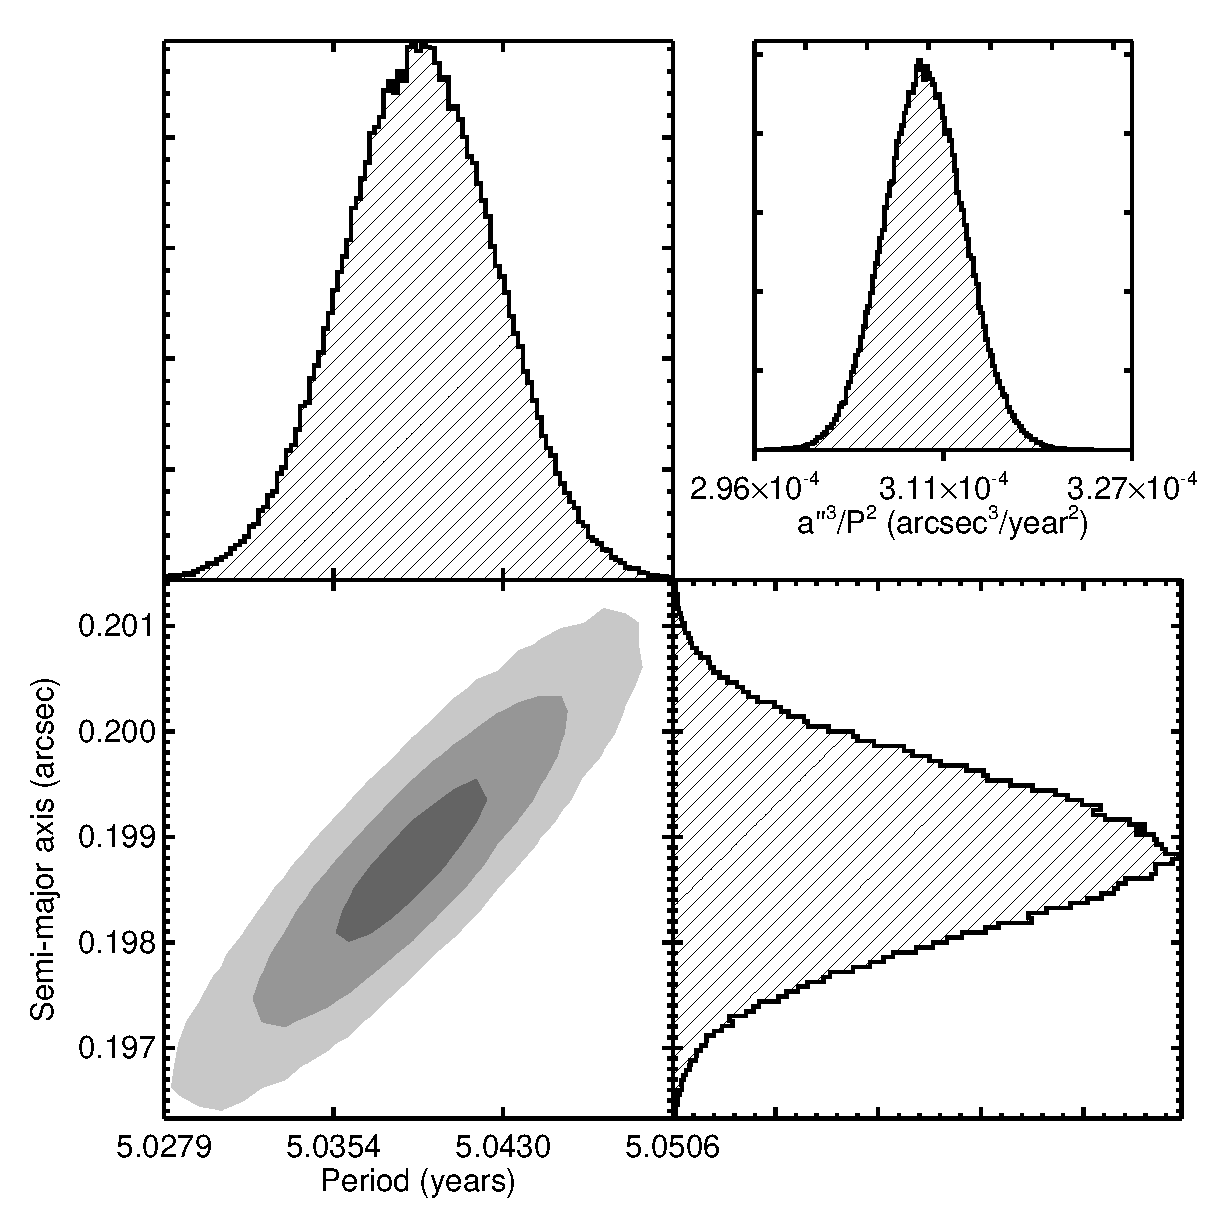
\includegraphics[width=0.47\textwidth]{LHS6167_corner.eps}
\caption{Example joint posterior on semi-major axis and orbital period (bottom left) for the system LHS 6167. Grey regions show 1, 2, and 3$\sigma$ (from darkest to lightest) of the points. The histograms above and to the right show the one-dimensional distributions of each parameter. The parameter fed into the \mmk\ fit is $a\arcsec^3/P^2$ (in arcsec$^3$ per year$^2$), which we show in the top right inset. }
\label{fig:correlated}
\end{center}
\end{figure}

For main-sequence dwarfs at fixed metallicity, more massive stars should always be brighter. Thus we required that the resulting fit have a negative derivative (higher \mks\ always gives lower mass) over the full range of input objects considered. We tested running without this constraint, and found similar results over most of the parameter range considered. The major difference was near the edges of the input sample. Without the negative derivative constraint, the fit would often become double valued where there were few points to constrain it.

To handle any variation not included in our formalism, we fit for an additional dimensionless parameter $\sigma_e$. This parameter was implemented as a fractional uncertainty in the total mass, added to the measurement uncertainty (from the orbit and parallax errors) in quadrature. $\sigma_e$ can be interpreted as missing physics (e.g., age, detailed abundances, and/or activity/rotation) driving an intrinsic scatter in the \mmk, or as underestimated uncertainties in our input parallaxes or orbital parameters (and hence the final assigned mass). We tested implementing similar missing error terms on the assigned $K$-band magnitudes (in case of stellar variability) or directly on the parallax priors, and found consistent results. We opted to keep $\sigma_e$ as a fractional error on the total mass, which we feel is more physically motivated.

\subsection{Results and Uncertainties}

We show the resulting posteriors for the polynomial coefficients ($a_i$) in Figure~\ref{fig:fitpost}. The spread in the posteriors for individual coefficients is large, suggesting significant errors on each coefficient. However, the coefficients are also highly correlated; for a given value assigned to four of the five fit coefficients, there is a relatively narrow set of solutions for the final constant. The final fit was tightly constrained over the full sequence, which we show in Figure~\ref{fig:relation} for individual masses, and combined masses in Figure~\ref{fig:m_m} (a more realistic representation of how the fit was done). 

\begin{figure*}[p]
\begin{center}
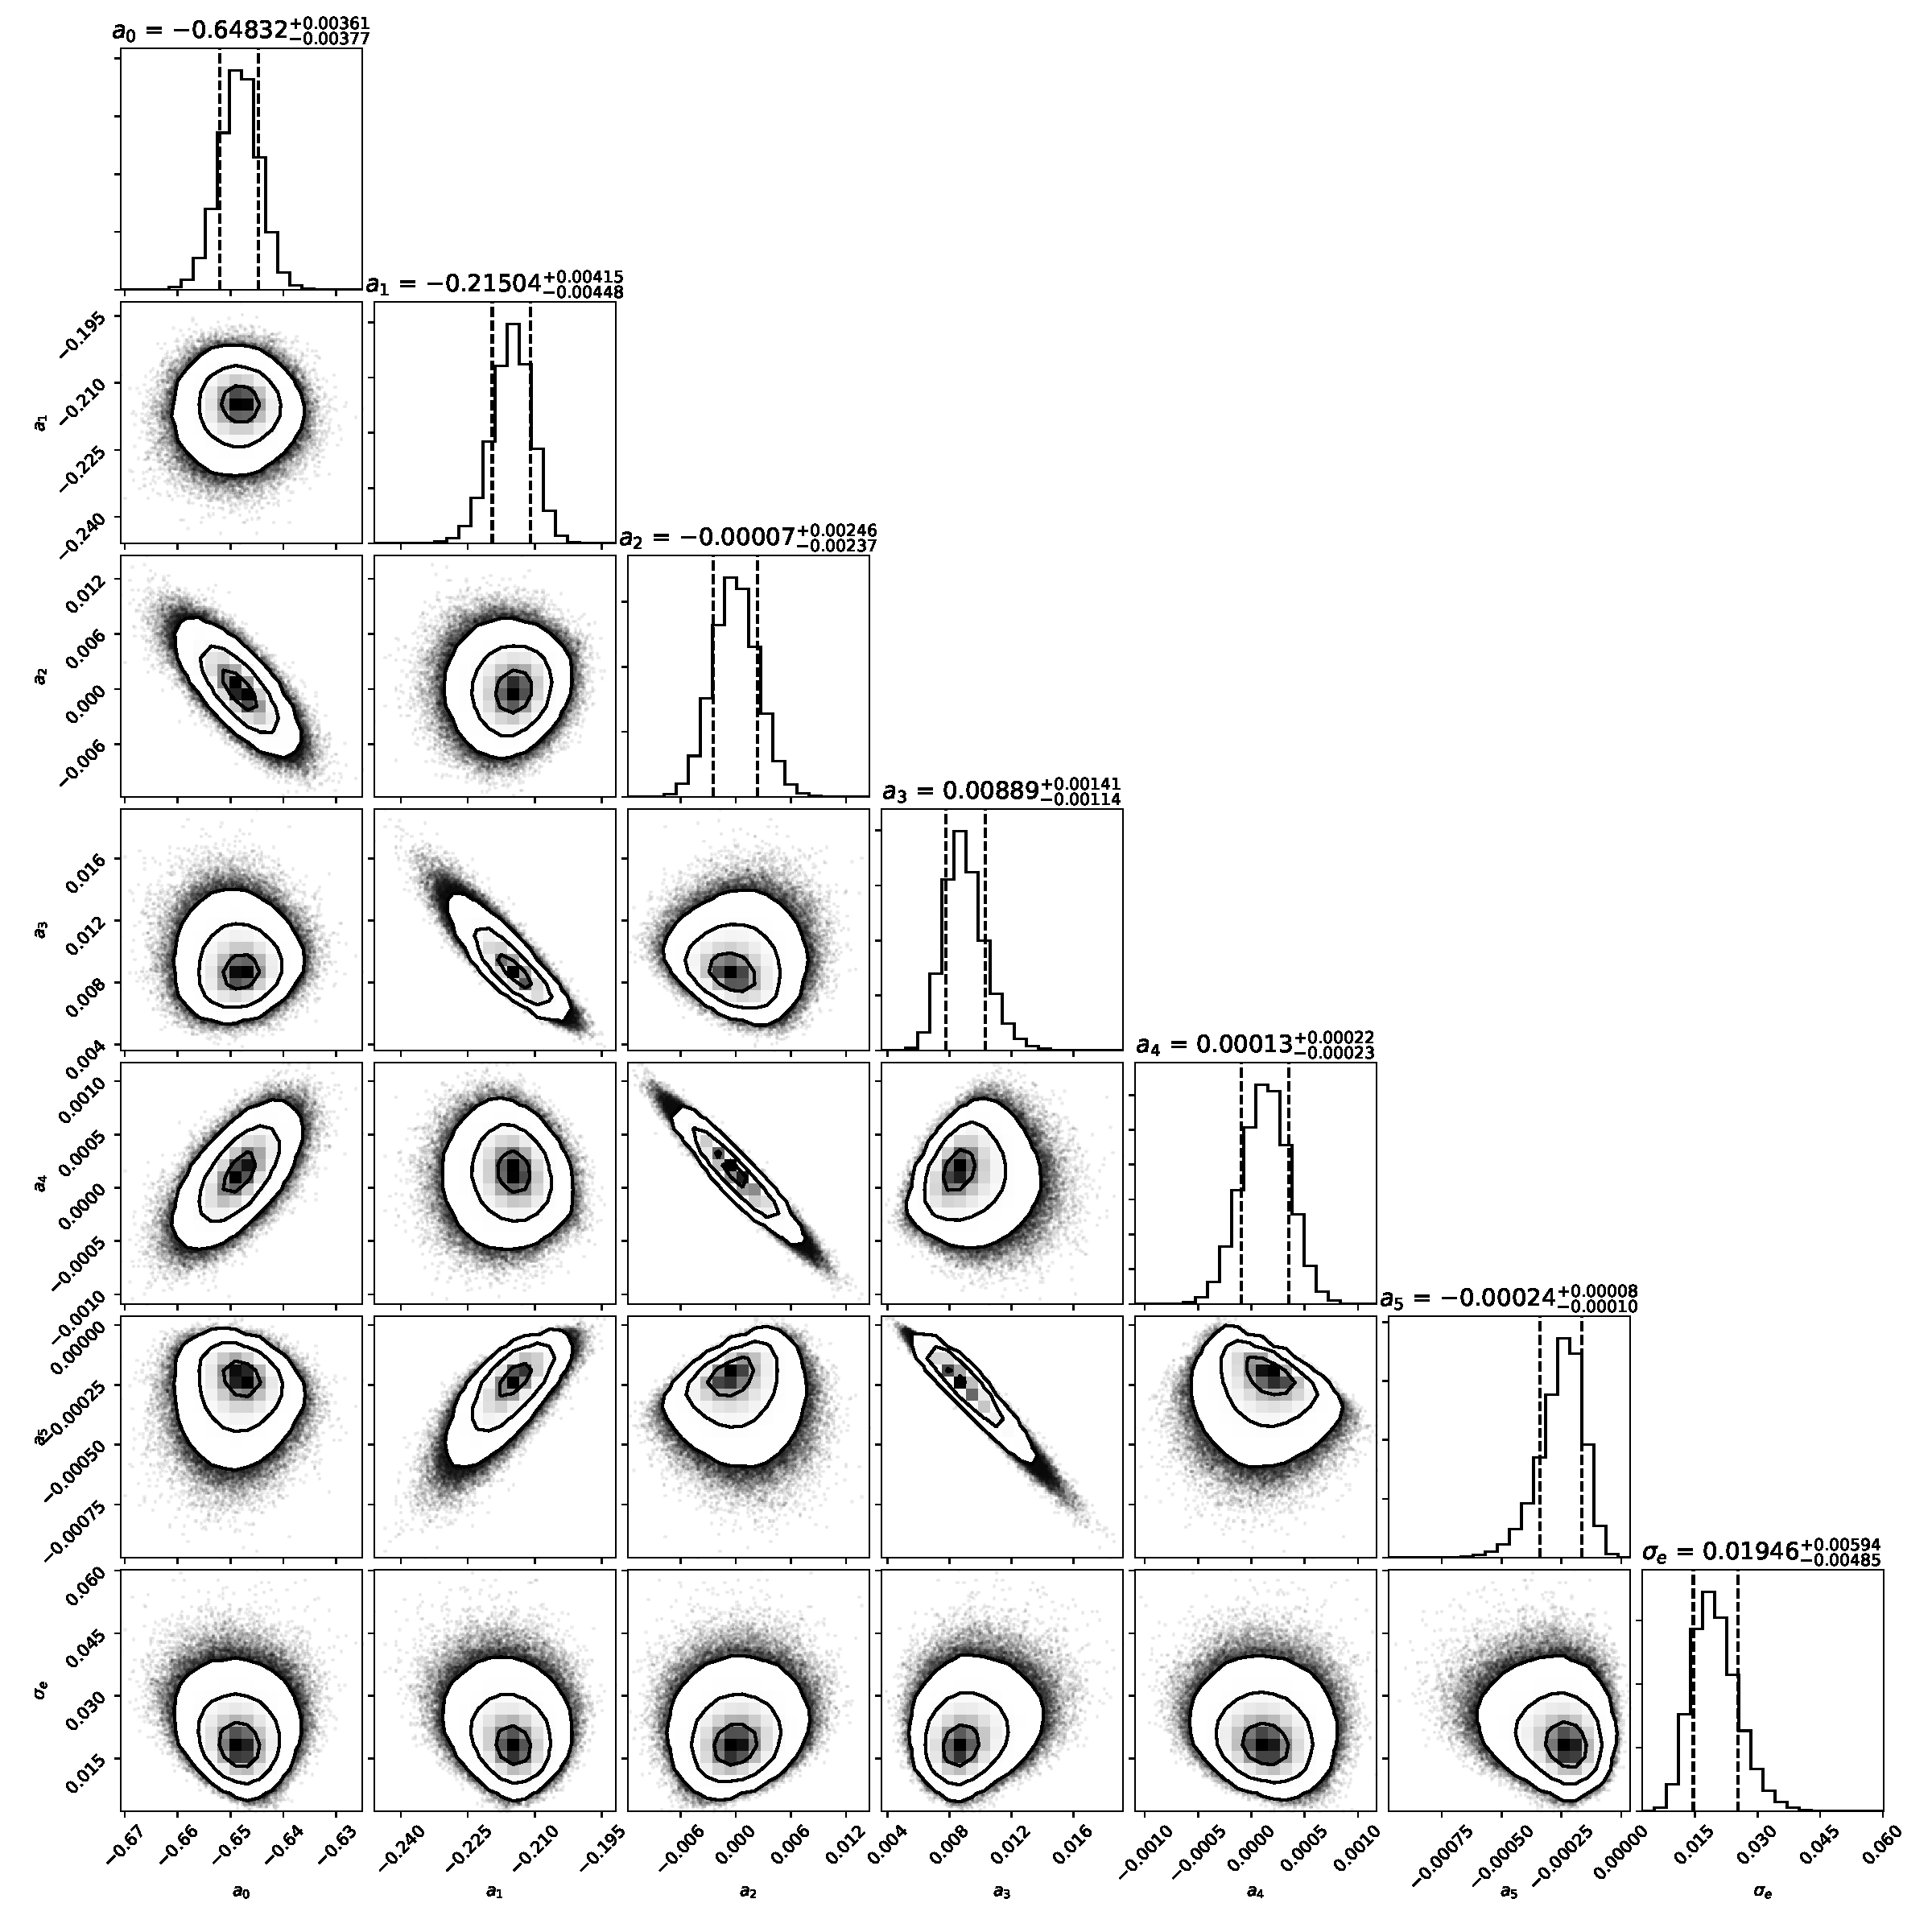
\includegraphics[width=0.9\textwidth]{output_7_eMs.pdf}
\caption{Posterior projections for the $a_i$ values derived from our MCMC fit to Equation~\ref{eqn:mmk2} as well as the additional error term $\sigma_e$. Contours denote the 1, 2, and 3$\sigma$ confidence intervals, and the dashed lines in the histogram mark 1$\sigma$. The $\sigma_e$ parameter represents the fractional error in the total mass, added to account for intrinsic variation in the relation or underestimated uncertainties in the input masses. Figure was generated using {\tt corner.py} \citep{corner}.}
\label{fig:fitpost}
\end{center}
\end{figure*}

\begin{figure*}[htp]
\begin{center}
\includegraphics[width=\textwidth]{MK_mass_0_7_1.eps}
\caption{Absolute $K_S$-band magnitude as a function of mass for targets in our sample (circles). Points are color-coded by their estimated metallicity. We show a typical error ellipse in grey to highlight that errors on mass and \mks\ measurements are correlated, and usually parallel to the $M_*$-\mks\ relation (both depend on the common parallax). The black dashed line indicates the best-fit (highest likelihood) from our MCMC analysis. To provide an estimate of the scatter in the relation as a function of mass, we show 100 randomly selected fits from the MCMC chain in grey. Note that our orbit fits only provide {\it total} mass; we used the mass ratios derived from the best-fit \mmk\ relation for the purposes of this figure. Figure~\ref{fig:m_m} shows the total mass comparison, which is more reflective of how the comparison is done. }
\label{fig:relation}
\end{center}
\end{figure*}

\begin{figure}[ht]
\begin{center}
\includegraphics[width=0.48\textwidth]{Mass_mass_7_0.eps}
\caption{Predicted total (system) $M_*$ from the \mmk\ relation as a function of the total mass determined from the orbit fit. Ellipses represent $\simeq1\sigma$ distribution of values for each point, accounting for parallax errors common to both the predicted and dynamical mass, but not accounting for scatter in the final \mmk\ relation ($\sigma_e$). Color-coding by [Fe/H] matches that of Figure~\ref{fig:relation}.}
\label{fig:m_m}
\end{center}
\end{figure}


Coefficients for powers of the same parity (even or odd) were strongly correlated to each other. This was expected, as a decrease in the slope (from linear) is best explained using an odd power, and increases with an even power. Coefficients for powers with even parity (with the exception of the $a_0$ term) were also generally centered around zero. This also was expected in the context of the shape of the relation seen in Figure~\ref{fig:relation}, and our requirement that the mass always decrease with decreasing luminosity (increasing \mks). A power with even parity will prefer to turn upwards at low masses. We explored this further by redoing the fit with no even powers (except $a_0$ was retained), but exploring higher-order odd powers. The resulting fit was significantly worse, with a $\sigma_e$ value twice as large compared fits with the same number of free parameters, but including even powers. The resulting fits also showed significant systematic deviations from the empirical data for $0.3M_\odot<M_*<0.5M_\odot$. We opted to include the even orders for all analyses despite their near-zero values. 

We adopted $n=\order$ as the preferred solution based both on the AIC values and visual inspection of the residuals. Lower-order fits did a reasonable job fitting most of the sequence, but poorly reproduced the masses of objects with $M_*<0.085M_\odot$. In this regime, the relation becomes increasingly non-linear. The result is that lower-order fits systematically overestimate the masses of the coolest objects in our sample (Figure~\ref{fig:order}) and tend to overestimate $\sigma_e$ to compensate. Higher-order fits explain the data reasonably well, but were not justified statistically (e.g., marginal decrease in $\sigma_e$) and showed slope changes outside the calibration sample that are not expected by theoretical considerations. 

\begin{figure}[h]
\begin{center}
\includegraphics[width=0.48\textwidth]{order.eps}
\caption{Fits of varying order ($n$) to Equation~\ref{eqn:mmk2} compared to the empirical values for the lowest-mass stars in our sample. The fits are similar above 0.085$M_\odot$, but a high-order ($n=\order$) is required to reproduce objects below this as the relation becomes increasing non-linear. The systematic offset seen between the low-mass sample and the best-fit relation can be seen in the coefficient posteriors as well as the best-fit relation (i.e., the distribution of fits are systematically high). }
\label{fig:order}
\end{center}
\end{figure}

We list the best-fit (highest likelihood) coefficient values in Table~\ref{tab:coeff}, as well as the median value of $\sigma_e$. We also provide trimmed posteriors for each coefficient in \href{https://github.com/awmann/M_-M_K-}{the github repository}. Fits using $n=4$ and $n=6$ are included in Table~\ref{tab:coeff} for reference, although we suggest using only the $n=\order$ relation. 

\begin{deluxetable*}{l l l l l l l l l l l l l l}
\tablecaption{Best-fit Coefficients for Equations~\ref{eqn:mmk2} and \ref{eqn:mmk3}}
\tablehead{
\colhead{$n$} & \colhead{$a_0$} & \colhead{$a_1$} & \colhead{$a_2$} & \colhead{$a_3$} & \colhead{$a_4$} & \colhead{$a_5$} & \colhead{$a_6$} & \colhead{f} & \colhead{$\sigma_e$ }
}
\startdata
4 & -0.65074 & -0.20234 & $  3.6638\rm{x}10^{-3}$ & $  5.0407\rm{x}10^{-3}$ & $ -2.6018\rm{x}10^{-4}$ & \nodata & \nodata & \nodata &  0.024\\
5 & -0.64661 & -0.21246 & $ -2.6534\rm{x}10^{-3}$ & $  7.9485\rm{x}10^{-3}$ & $  3.6899\rm{x}10^{-4}$ & $ -1.9226\rm{x}10^{-4}$ & \nodata & \nodata &  0.019\\
6 & -0.63910 & -0.20981 & $ -1.2332\rm{x}10^{-2}$ & $  6.8080\rm{x}10^{-3}$ & $  2.5023\rm{x}10^{-3}$ & $ -1.0325\rm{x}10^{-4}$ & $ -1.2146\rm{x}10^{-4}$ & \nodata &  0.018\\
\hline
4 & -0.65123 & -0.20169 & $  4.7567\rm{x}10^{-3}$ & $  4.9324\rm{x}10^{-3}$ & $ -2.9132\rm{x}10^{-4}$ & \nodata & \nodata &  0.0360 &  0.024\\
5 & -0.64177 & -0.21493 & $ -5.5294\rm{x}10^{-3}$ & $  8.9387\rm{x}10^{-3}$ & $  6.3228\rm{x}10^{-4}$ & $ -2.7022\rm{x}10^{-4}$ & \nodata &  0.0380 &  0.018\\
6 & -0.64145 & -0.21410 & $ -8.4574\rm{x}10^{-3}$ & $  7.7961\rm{x}10^{-3}$ & $  1.5020\rm{x}10^{-3}$ & $ -1.5918\rm{x}10^{-4}$ & $ -5.3935\rm{x}10^{-5}$ &  0.0307 &  0.018\\
 \enddata
\label{tab:coeff}
\tablecomments{The $n=5$ fit is preferred independent of including [Fe/H]. Note that values presented here are the highest likelihood for the $a_i$ values, with the median value for $f$ and $\sigma_e$. Figures~\ref{fig:fitpost} and \ref{fig:fitpost_feh} note the median coefficient values.}
\end{deluxetable*}

To estimate the uncertainty in the relation we computed the standard deviation in the derived masses for a fixed \mks\ across all MCMC steps, which we report in Table~\ref{tab:err}. In the best-constrained regions ($5\lesssim$\mks$\lesssim7$, $0.3\lesssim M_*\lesssim0.6$) the scatter in the relation is $\lesssim$1\%, reaching $\simeq$3\% near the edges. These values in Table~\ref{tab:err} could potentially be used as a reference for estimating errors on the output mass for a given \mks\ if combined with errors from the distance and $K_S$ magnitude. This does not account for intrinsic scatter in the \mmk\ relation. To this end, we performed the sample calculation, but included $\sigma_e$ as an estimate of any intrinsic scatter in the relation. It is possible that $\sigma_e$ is purely a representation of missing uncertainties in the input parameters (e.g., orbital parameters, parallaxes, $K_S$). However, even in this case, we cannot rule out the presence of intrinsic variation at the level of $\sigma_e$ without removing (or at least characterizing) the missing errors captured within $\sigma_e$. We advise using the errors that include $\sigma_e$ for all mass uncertainty estimates.

\begin{deluxetable}{l l l | l l | l l}
\tablecaption{Error in \mmk\ Relation}
\tablehead{
 \colhead{$M_{K_S}$} & \colhead{$M_*$} & \colhead{SpT$^a$} & \colhead{$\sigma_{M_*}^b$} & \colhead{$\sigma_{M_*}^b$} & \colhead{$\sigma_{M_*}^c$} & \colhead{$\sigma_{M_*}^c$}  \\
 \colhead{(mag)} & \colhead{$M_\odot$} & \colhead{} & \colhead{$M_\odot$} & \colhead{\%} & \colhead{$M_\odot$} & \colhead{\%} 
}
\startdata
\multicolumn{7}{c}{No [Fe/H] term ($f=0$), 5th order} \\
\hline
 4.0 & 0.742 & K4.5 & 0.028 & 0.038 & 0.031 & 0.042\\
 4.5 & 0.669 & K7.0 & 0.011 & 0.017 & 0.017 & 0.026\\
 5.0 & 0.6004 & M0.0 & 0.0091 & 0.015 & 0.015 & 0.025\\
 5.5 & 0.5248 & M1.5 & 0.0067 & 0.013 & 0.012 & 0.023\\
 6.0 & 0.4430 & M2.5 & 0.0046 & 0.010 & 0.0098 & 0.022\\
 6.5 & 0.3615 & M3.0 & 0.0034 & 0.010 & 0.0078 & 0.022\\
 7.0 & 0.2871 & M3.5 & 0.0026 & 0.009 & 0.0062 & 0.021\\
 8.0 & 0.1759 & M4.5 & 0.0016 & 0.009 & 0.0038 & 0.021\\
 8.5 & 0.1398 & M5.0 & 0.0014 & 0.010 & 0.0031 & 0.022\\
 9.0 & 0.1143 & M6.0 & 0.0013 & 0.011 & 0.0026 & 0.022\\
 9.5 & 0.0971 & M6.5 & 0.0012 & 0.013 & 0.0023 & 0.023\\
10.0 & 0.0860 & M7.5 & 0.0013 & 0.015 & 0.0021 & 0.025\\
10.5 & 0.0791 & M9.0 & 0.0013 & 0.016 & 0.0020 & 0.025\\
11.0 & 0.0745 & L1.0 & 0.0019 & 0.025 & 0.0024 & 0.032\\
\hline
\multicolumn{7}{c}{[Fe/H] term ($f$), 5th order} \\
\hline
 4.0 & 0.753 & K4.5 & 0.029 & 0.039 & 0.032 & 0.043\\
 4.5 & 0.671 & K7.0 & 0.011 & 0.016 & 0.017 & 0.025\\
 5.0 & 0.5990 & M0.0 & 0.0091 & 0.015 & 0.014 & 0.024\\
 5.5 & 0.5231 & M1.5 & 0.0067 & 0.013 & 0.012 & 0.022\\
 6.0 & 0.4423 & M2.5 & 0.0045 & 0.010 & 0.0093 & 0.021\\
 6.5 & 0.3618 & M3.0 & 0.0035 & 0.010 & 0.0075 & 0.021\\
 7.0 & 0.2880 & M3.5 & 0.0027 & 0.009 & 0.0059 & 0.021\\
 8.0 & 0.1769 & M4.5 & 0.0016 & 0.009 & 0.0036 & 0.021\\
 8.5 & 0.1405 & M5.0 & 0.0015 & 0.010 & 0.0030 & 0.021\\
 9.0 & 0.1147 & M6.0 & 0.0013 & 0.011 & 0.0025 & 0.022\\
 9.5 & 0.0974 & M6.5 & 0.0013 & 0.013 & 0.0022 & 0.022\\
10.0 & 0.0862 & M7.5 & 0.0013 & 0.015 & 0.0020 & 0.024\\
10.5 & 0.0794 & M9.0 & 0.0013 & 0.016 & 0.0020 & 0.025\\
11.0 & 0.0750 & L1.0 & 0.0018 & 0.024 & 0.0023 & 0.030\\
\enddata
\label{tab:err}
\tablecomments{This table assumes \mks\ (and [Fe/H]) are known perfectly. Total errors on $M_*$ should take into account errors in the measured parameters and the relation. }
\tablenotetext{$a$}{Spectral types are given for reference, but are extremely rough because of a significant dependence on metallicity and how the spectral typing is done (e.g., which indices are used, NIR versus optical). It is not recommended to use this table as a means to compute \mks\ or $M_*$ from a spectral type or vice versa. }
\tablenotetext{$b$}{The uncertainty in the resulting $M_*$ at a given $M_{K_S}$ ignoring $\sigma_e$}
\tablenotetext{$c$}{The uncertainty in the resulting $M_*$ at a given $M_{K_S}$ accounting for $\sigma_e$}
\end{deluxetable}

A more robust account of errors than using Table~\ref{tab:err} would be to use the full coefficient posteriors to account for asymmetry around the best-fit relation (i.e., by sampling a range of possible $a_i$ values). To aid with this, we included the fit posteriors and a simple \href{https://github.com/awmann/M_-M_K-}{code} that provides output $M_*$ posteriors given a $K_S$, distance, and associated uncertainties. The program combines the scatter in the coefficients with the median value of $\sigma_e$ to produce a realistic $M_*$ posterior (including assymetry). Over most of the relation, particularly $0.1M_\odot<M_*<0.5M_\odot$, $\sigma_e$ is the dominant source of uncertainty in estimating masses. 

\subsection{The role of metallicity}\label{sec:metal}

We explored the the effects of [Fe/H] on the \mmk\ relation using the Mesa Isochrones and Stellar Tracks \citep[MIST,][]{MIST0,MIST1}. We also tested models from the Dartmouth Stellar Evolution Database \citep[DSEP,][]{Dotter2008}, and found results to be broadly in agreement. We preferred MIST because their model atmospheres include a newer set of molecular lines (e.g., TiO) that are important in M dwarfs and may impact the synthetic photometry. The Lyon models \citep[BHAC15,][]{BHAC15} employ a model atmosphere in reasonable agreement with nearby stars with interferometrically determined \teff\ values \citep{Boyajian2012,Mann2013c}, and go to lower masses than DSEP and MIST. However, the BHAC15 models cover only solar metallicity. 

We show the expected \mks\ tracks from MIST for different metallicities in Figure~\ref{fig:mk_metal} alongside our empirical determinations. MIST models do not extend below 0.1$M_\odot$, so we restricted our comparison to above that mass. For this comparison we assumed a fixed age of 5\,Gyr, although the choice of age from 1-10\,Gyr makes a negligible difference for the mass range shown (Figure~\ref{fig:age}). 

Note that metal-rich stars are expected to be {\it less luminous} for a fixed $M_*$, whereas the opposite trend is seen for a fixed \teff\ and most color selections. Higher metal abundance increases the stellar radius for a fixed $M_*$ (because of higher opacity), which lowers the density and pressure near the core, decreasing the overall rate of fusion and hence the total luminosity. This effect is mitigated somewhat at $K$-band, because high [Fe/H] mostly increases opacity in the optical, causing more flux to escape at NIR wavelengths (in Figure~\ref{fig:metal}, the metal-rich spectrum sits low in the optical and high in the NIR when compared to the Solar-metallicity spectrum). 

Above 0.4$M_\odot$ there is a slight trend for metal-rich stars in our sample to land below the median sequence, as expected from the models. However, many metal-poor stars also land below the sequence, and there is no obvious trend below 0.4$M_\odot$. Further, the largest metal-rich outlier in the high-mass region (Gl 99) had a relatively poor mass determination (13\%). 

\begin{figure}[htp]
\begin{center}
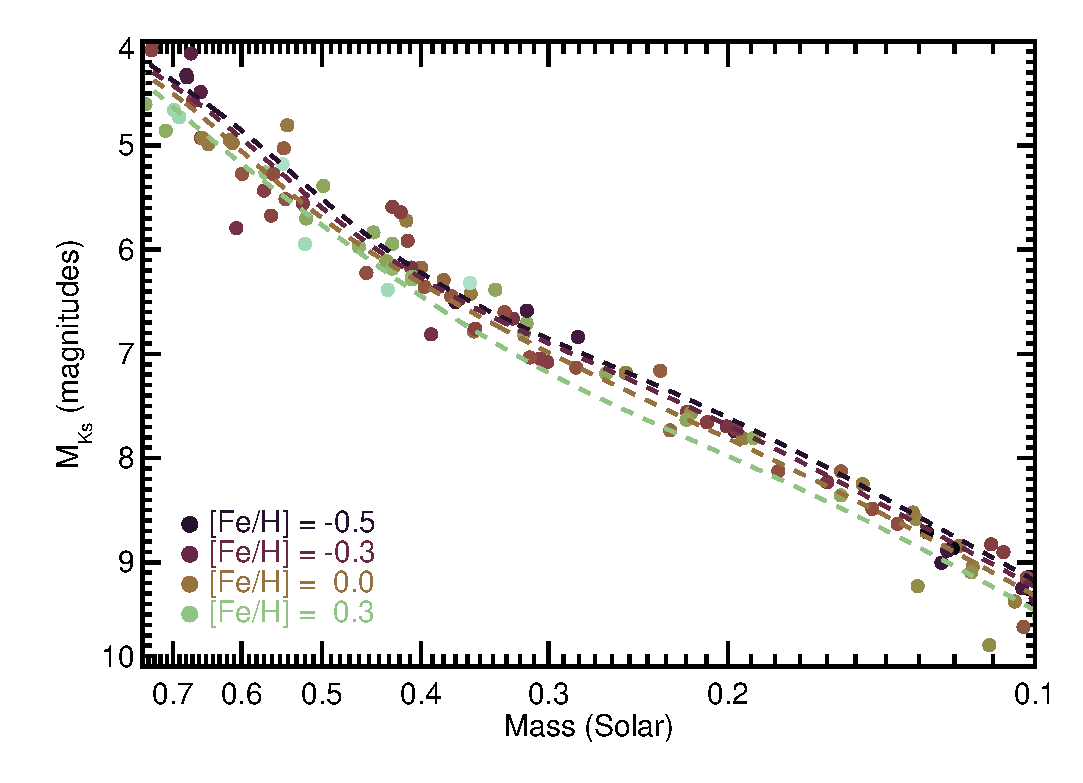
\includegraphics[width=0.47\textwidth]{Model_metal_0.eps}
\caption{\mks\ as a function of $M_*$ using MIST tracks of different metallicities (dashed lines) compared to empirical mass determinations (points). Color-coding by metallicity is the same for the points and lines, and matches the color scale of Figure~\ref{fig:relation}. The plot cuts at 0.1$M_\odot$, as the MIST models do not go below this limit. }
\label{fig:mk_metal}
\end{center}
\end{figure}

The residuals from our best-fit relation confirmed a weak (or no) effect on the derived $M_*$ due to changes in [Fe/H], as we show in Figure~\ref{fig:metal_resid}. A Spearman's rank test yielded no significant correlation between the residuals and [Fe/H]. We tried resampling the measurements using their uncertainties, and $<$1\% of samples showed a significant correlation. We also repeated this test, but restricted to just the best-characterized systems ($<5\%$ precision on mass) and still found no significant trend with [Fe/H]. 

\begin{figure}[htp]
\begin{center}
\includegraphics[width=0.47\textwidth]{residual_metal7.eps}%% needs to be replaced
\caption{Fractional difference between the orbital and predicted system mass as a function of metallicity of the system. The top panel contains all systems, while the bottom shows just those with $<$5\% uncertainties on $M_*$. Points are color-coded by the masses of components, with the inner dot corresponding to the primary star's estimated mass, and the outer circle the companion's estimated mass. Errors consider only input errors on total $M_*$.}%Quoted errors in mass account for the scatter in the \mmk\ relation.} 
\label{fig:metal_resid}
\end{center}
\end{figure}

Our sample is limited in its [Fe/H] range; 64\% of the targets are $-0.2<$[Fe/H]$<+0.2$ and only one target has [Fe/H]$<-0.5$. It is possible that our best-fit relation masked any [Fe/H] term by shifting the fit to match the typical metallicity of stars at a given \mks. We explored this by fitting for a term in [Fe/H] of the form:
\begin{eqnarray}\label{eqn:mmk3}
M_{tot} &=& (1+f[\rm{Fe/H]})\left(10^{b_1} + 10^{b_2}\right),
\end{eqnarray}
where $b_j$ is defined in Equation~\ref{eqn:mmk2_b}. This form assumes that a linear change in [Fe/H] corresponds to a fractional change in $M_*$ (e.g., f=0.1 would correspond to a 10\% change in derived $M_*$ per dex in [Fe/H] for a fixed \mks). This is generally consistent with the evolutionary models, although there is a small change in the scale ($f$) over the range of masses considered here. 

For this analysis we excluded the two L dwarfs from the sample because their metallicities are less reliable (extrapolated from an M dwarf calibration). As with our fit to Equation~\ref{eqn:mmk2}, we tested a range of values for $n$ (number of $a_i$ coefficients). Our MCMC fitting method was otherwise identical to that outlined in Section~\ref{sec:relation}. Since we were primarily interested in the {\it relative} effect of [Fe/H], and not necessarily the absolute scale, we assumed the smaller (relative) errors on [Fe/H] (see Section~\ref{sec:feh}). 

We show the output coefficient posteriors in Figure~\ref{fig:fitpost_feh} and list the best-fit coefficients in Table~\ref{tab:coeff}. As with our fits neglecting $f$, we found significantly better agreement with the lowest-mass objects in the sample using $n=\order$, although $n=4$ and $n=6$ are listed in Table~\ref{tab:coeff} for reference. 

\begin{figure*}[p]
\begin{center}
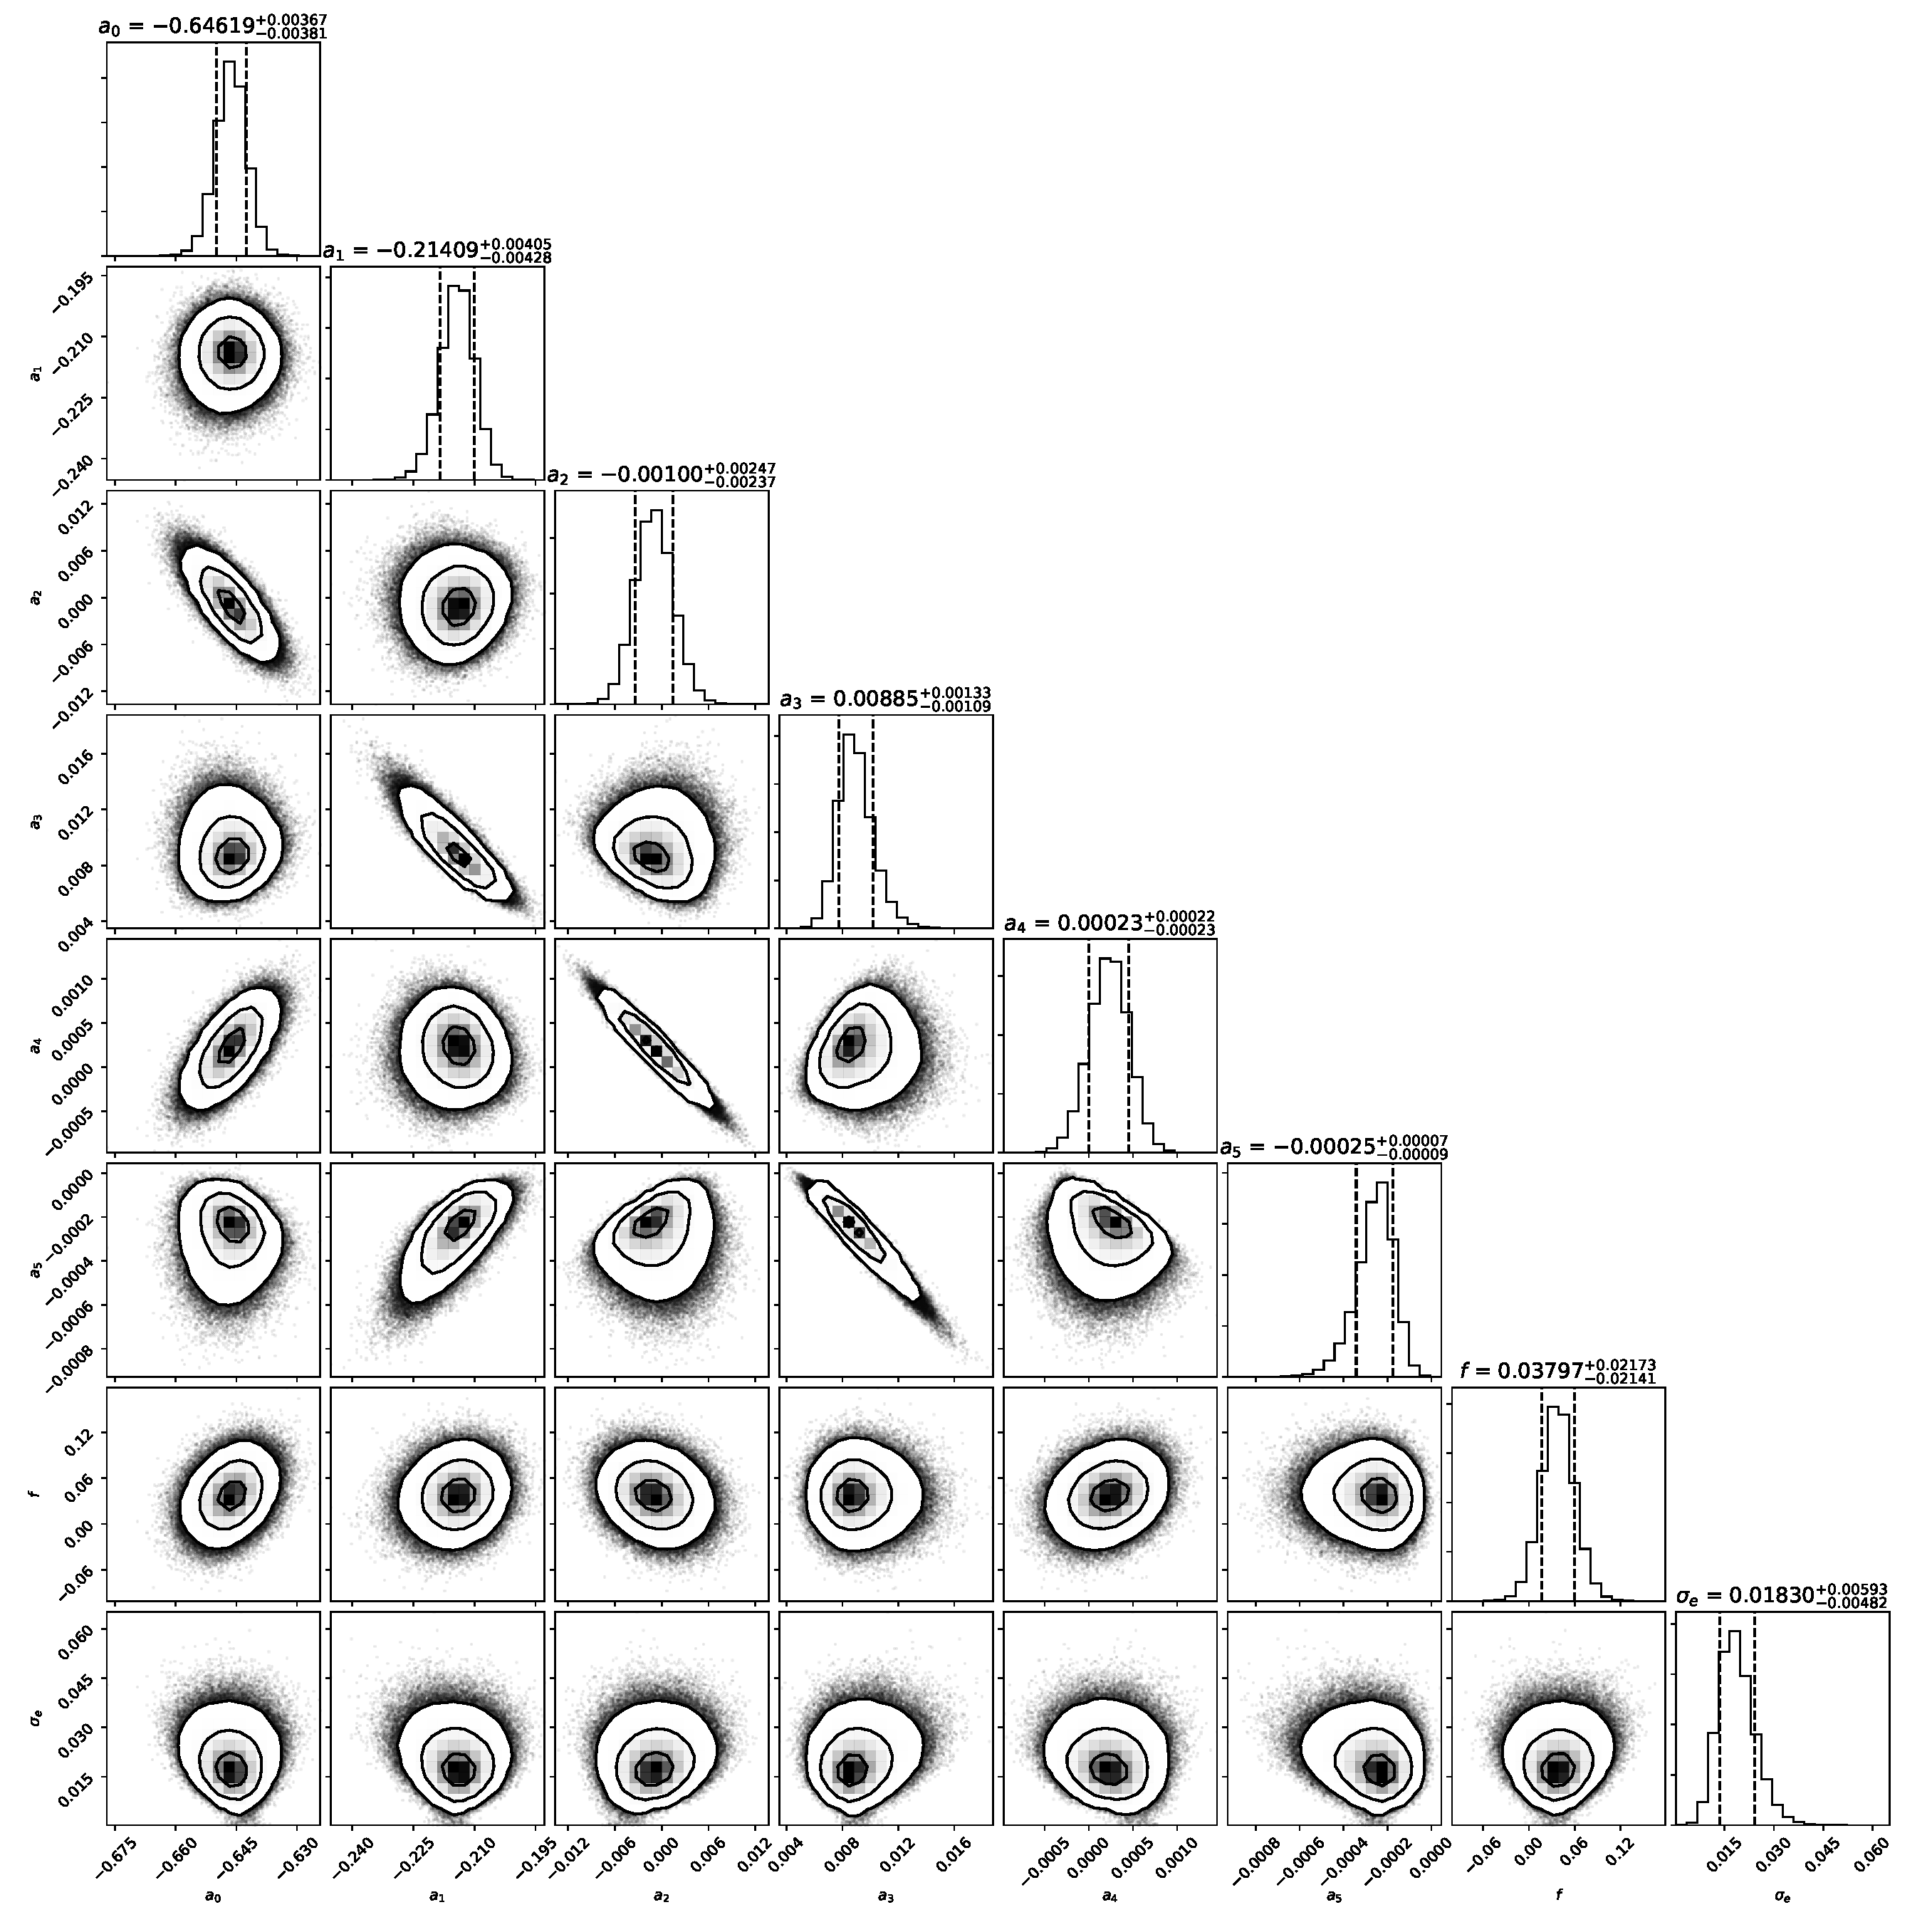
\includegraphics[width=0.97\textwidth]{output_8feh_eMs.pdf}
\caption{Same as Figure~\ref{fig:fitpost}, but for the fit following Equation~\ref{eqn:mmk3}, i.e., including the [Fe/H] term, $f$. }
\label{fig:fitpost_feh}
\end{center}
\end{figure*}

Consistent with our previous analysis, our $f$ value is consistent with zero (no impact of [Fe/H] on the \mmk\ relation) at 1.7$\sigma$. This suggests our relation will work reasonably well even on more extreme metallicity samples (e.g., Halo stars). However, it is also possible that [Fe/H] is less important than abundances of elements that specifically impact the strength of molecular features in M dwarf spectra. Higher C/O, for example, suppresses available Oxygen for TiO formation, weakling a major source of opacity in the optical \citep[e.g., C, O, Ti,][]{2012ApJ...747L..27F,2015ApJ...804...40G,Veyette2016a}. This also might explain some of the extra scatter in the relation ($\sigma_e$) if there is sufficient variance of these abundances in the given sample. Testing this will require a means to determine more detailed abundances of M dwarfs \citep[e.g.,][]{Veyette2017}, and/or to add in subdwarf binaries or other systems with more extreme abundances to provide increased leverage on any metallicity effects. 

To compare to the models, we fit the MIST grid points in the same manner as the empirical dataset following Equation~\ref{eqn:mmk3}. In Figure~\ref{fig:f} we show the posterior on $f$ from the model grid compared to that from the dynamical masses. The models predict a significantly larger [Fe/H] effect then supported by our binary sample. The difference between the two posteriors ($f_{\rm{model}}-f_{\rm{dynamical}}$) is greater than zero at $4.1\sigma$. 

\begin{figure}[htp]
\begin{center}
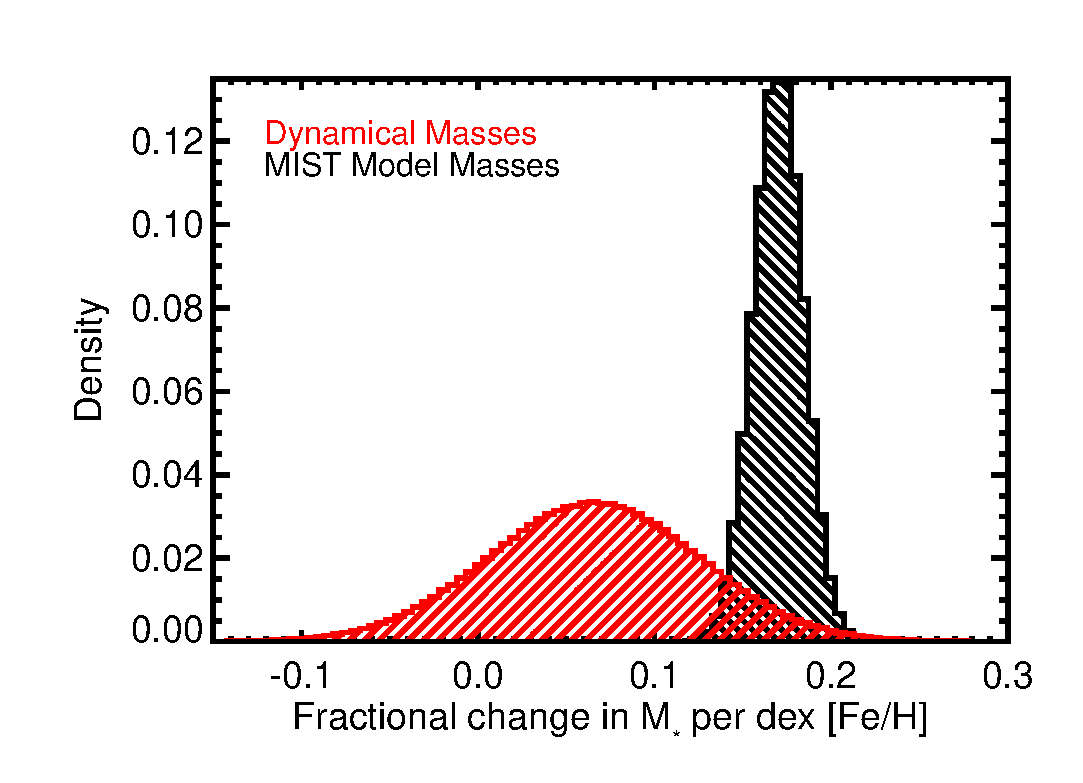
\includegraphics[width=0.47\textwidth]{F_plot.eps}
\caption{Comparison of the posterior on $f$ (fractional change in $M_*$ per dex in metallicity for a fixed \mks; Equation~\ref{eqn:mmk3}) predicted by the MIST models (black) compared to that using our dynamical masses (red). There are an identical number of points in each posterior and the bin sizes are the same. }
\label{fig:f}
\end{center}
\end{figure}

The difference between model and empirical predictions for $f$ holds for different subsets of the data and accounting for potential systematics in the assigned [Fe/H]. There is some evidence in the binary sample that [Fe/H] effects are stronger at the high-mass end (see Figure~\ref{fig:relation}). We tested this by repeating the analysis excluding binaries with one or more component masses below $0.35M_\odot$. While we found a marginally larger $f$ value using just the higher-mass sample ($f=0.056\pm0.035$\,dex$^{-1}$), this was still 2.5$\sigma$ discrepant from the model prediction and consistent with the result from the entire binary sample at $<1\sigma$. The difference also held if we restrict our sample to $0.1<M_\odot<0.6$, where the M dwarf [Fe/H] relations are best calibrated \citep{Mann2013a,Mann2014}.

The model discrepancy also cannot be explained by $\sigma_e$. Whatever interpretation we apply to this value, it only amounts to $\simeq$2\% variation in $M_*$ for a given \mks. The models predict a metallicity effect of $\simeq0.17$ per dex, and since our sample covers about 1 dex in [Fe/H], this translates to an expected $\simeq$17\% variation in mass over the full sample, or 8\% if we just consider the majority of the targets. It is possible that $\sigma_e$ is being driven in part by erroneous assigned [Fe/H] (or underestimated errors on [Fe/H]) which could decrease our derived $f$ value, but the effect is too small to reconcile with the models. 

Overestimating the effect of [Fe/H] may be related to missing opacity/molecular lines in the atmospheric models. Missing opacity at optical wavelengths could strengthen the effect of [Fe/H] by underestimating the number of saturated features (if a line is saturated adding [Fe/H] cannot make it stronger). The effect at NIR wavelengths would be weaker, since there are fewer molecular bands, but underestimated opacity in the optical would also change the continuum levels in the NIR as well as how those levels change with [Fe/H]. 

If the issue is related to the atmospheric models, the effect should change as a function of mass/\teff\ as molecular lines become stronger with decreasing temperature. However, this is hard to test with the current sample, since we do not have a large spread in [Fe/H] when compared to the [Fe/H] measurement uncertainties over the full mass range. Recent comparison suggest models reproduce optical and NIR spectra of M dwarfs to $\simeq$5\% \citep[e.g.,][]{Lepine:2013,Mann2013c}, with the exception of a few molecular features like CaOH, AlH, and NaH \citep{Rajpurohit:2013}. These bands are mostly blueward of 6000\AA, so blue flux ratios of our targets could help test this, as well as adding in more extreme metallicity systems. Erroneous model continuum opacities could have a larger effect than individual missing lines or molecular bands. Poor continuum opacities are usually absorbed into normalization parameters \citep[e.g.,][]{Cushing:2008fj}, and hence difficult to test without direct constraints on the radius, such as those from long-baseline optical interferometry \citep[e.g.,][]{Boyajian2015,Kane2017}.

\subsection{Comparison to previous relations}\label{sec:other}

\subsubsection{\citet{Delfosse2000}}

\citet{Delfosse2000} provided one of the most commonly used \mmk\ relations, covering $0.1M_\odot<M_*<0.6M_\odot$. Like our work, the calibration was built primarily on astrometric binaries. Nearly all the targets in \citet{Delfosse2000} were included in our sample, with the exception of triple systems and eclipsing binaries, both of which we avoided because of the complexity of computing total masses in the first scenario and in the latter, estimating \mks\ and the effect of tides and enhanced activity on the radii of stars on short-period, eclipsing orbits. Because of the sample overlap, consistency is expected. However, a comparison can be useful to see how past use of \citet{Delfosse2000} may change with our more precise results.

We show the comparison in Figure~\ref{fig:delfosse}, including the points used in the \citet{Delfosse2000} calibration as well as the two fit lines. Given errors often quoted for the \citet{Delfosse2000} relation (5-10\%), the two fits are in remarkable ($<$5\%) agreement over most of the mass range ($0.15M_\odot \lesssim M_* \lesssim 0.5M_\odot$). Only at the high-mass end do the two relations diverge by as much as 10\%, but \citet{Delfosse2000} had few calibrators in this regime. While the two relations are in excellent agreement, the relation presented here is a factor of 2-5$\times$ more precise over the whole mass regime. 

\begin{figure}[htb]
\begin{center}
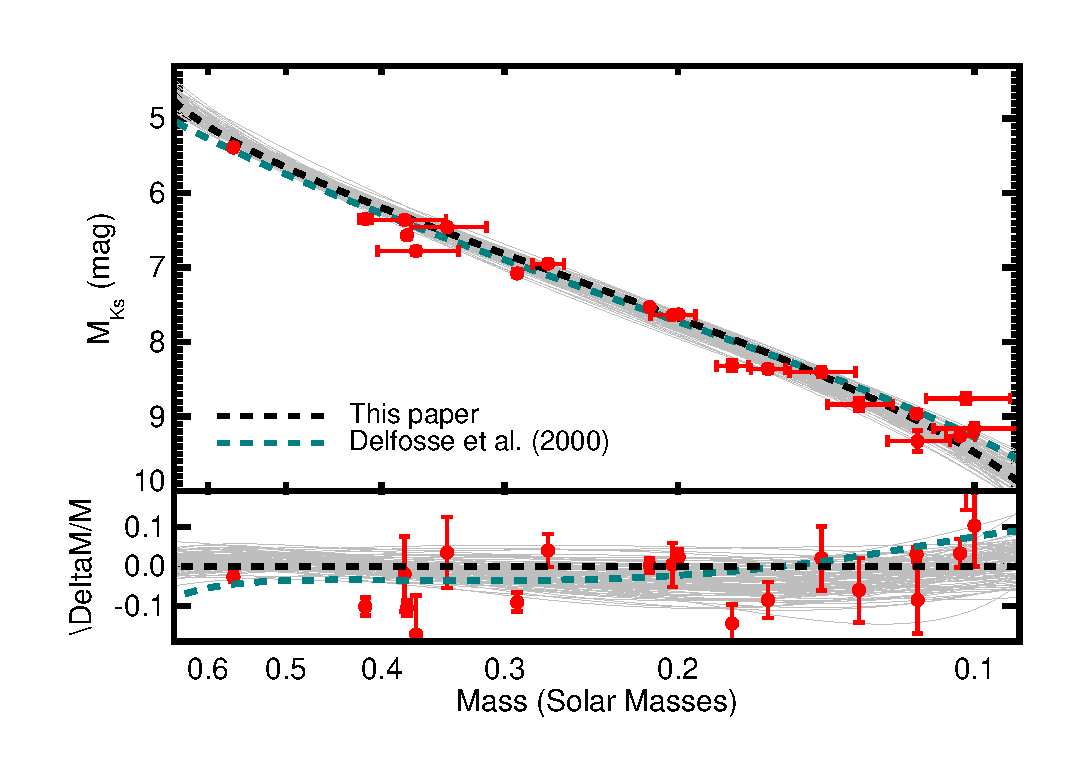
\includegraphics[width=0.47\textwidth]{Delfosse_comp.eps}
\caption{Absolute $K_S$-band magnitude as a function of mass for astrometric binaries analyzed by \citet{Delfosse2000} (red circles). The resulting $M_*$-\mks\ relation from \citet{Delfosse2000} is shown as a teal dashed line, while the best-fit relation from this paper is shown as a blacked dashed line (with error in grey as in Figure~\ref{fig:relation}). The bottom panel shows the residual of the \citet{Delfosse2000} points compared to our relation.}
\label{fig:delfosse}
\end{center}
\end{figure}

\subsubsection{\citet{Mann2015b}}

\citet{Mann2015b} built a catalog of 183 M dwarfs with precise \teff\ and $R_*$, calibrated against radii measurements from long-baseline optical interferometry \citep{Boyajian2012} and precision bolometric fluxes \citep[e.g.,][]{Mann2015a,2015MNRAS.447..846B}. Masses were computed for these stars by interpolating the parameters onto an updated version of the DSEP models as described in \citet{Feiden2013,Feiden2014} and \citet{Muirhead2014}. Although these masses were model-dependent, they accurately reproduced the mass-radius relation from low-mass eclipsing binaries. This suggested that the model-based masses were accurate to $\simeq$3\% or better, and motivated the development of a \mmk\ relation from the \citet{Mann2015b} sample. A comparison to our relation can be seen in part as a test on the updated DSEP models, in addition to the results given in \citet{Mann2015b}. 

We show our fit with uncertainties alongside \citet{Mann2015b}'s in Figure~\ref{fig:mann}. The two fits track each other extremely well, with a maximum divergence of $\simeq$5\%. Given the quoted 2-3\% uncertainties from \citet{Mann2015b} and the 2-3\% errors in our relation, this difference is not significant. There is a hint of tension at the high-mass end, where our MCMC posterior is asymmetric, and at 0.2-0.3$M_\odot$ where the difference is the largest, but never does the the offset exceed the estimated uncertainties. 

\begin{figure}[htb]
\begin{center}
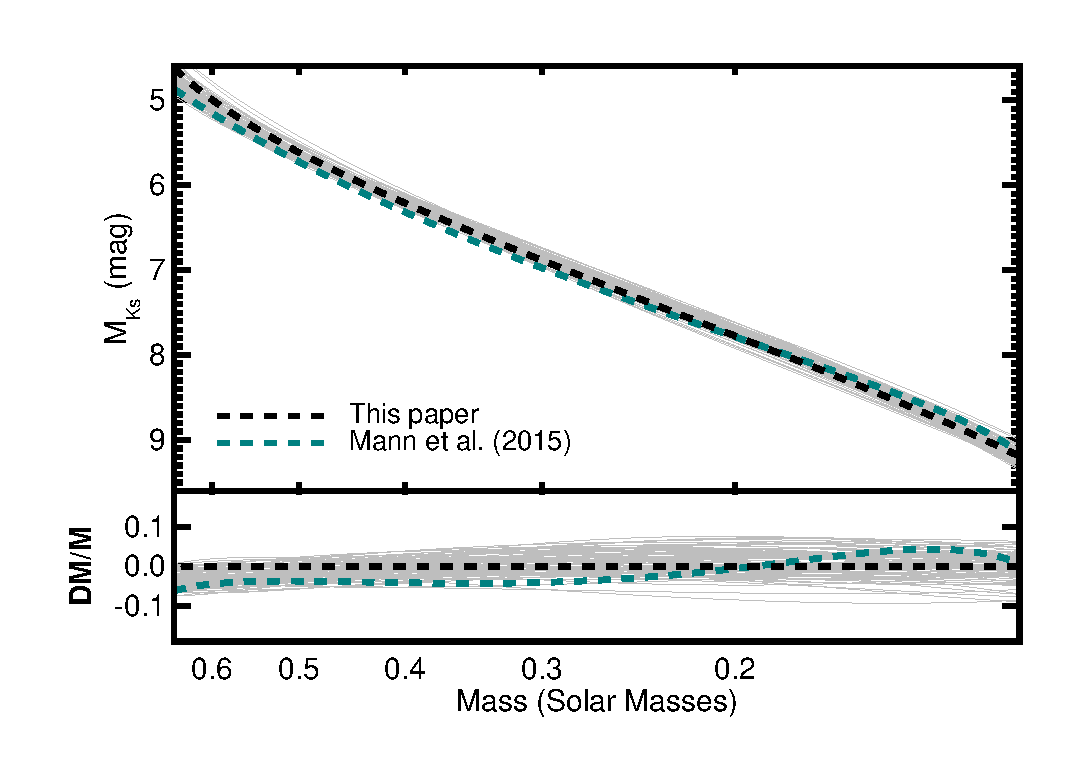
\includegraphics[width=0.47\textwidth]{Mann_comp.eps}
\caption{Comparison of $M_*$-\mks\ from \citet{Mann2015b}, shown as a teal dashed line, to that from this paper, which is shown in black, with 100 randomly selected realizations of the MCMC (as with Figures \ref{fig:relation} and \ref{fig:delfosse}). Residual is shown in the bottom panel. Individual points from \citet{Mann2015b} on which the calibration is based are not shown (for clarity), but they follow a tight sequence around the teal line. Only the range of masses covered by \citet{Mann2015b} are shown. }
\label{fig:mann}
\end{center}
\end{figure}


\subsubsection{\citet{Benedict2016}}
Like our work, the \citet{Benedict2016} relation was also based primarily on masses derived from M dwarf astrometric binaries. The \citet{Benedict2016} sample uses absolute astrometry from {\it HST} fine guidance sensors and radial velocities for a subset of systems. In addition to the precision provided by {\it HST}, this combination yields individual (component) masses, and, in many cases, independent constraints on parallaxes. So although our sample is larger and contains most of the targets in \citet{Benedict2016}, their analysis is not subject to many of the complications of our own. 

We compare our \mmk\ relation \citet{Benedict2016}'s in Figure~\ref{fig:benedict}. The two relations are in excellent agreement for $0.09M_\odot\lesssim M_* \lesssim 0.25M_\odot$. Below this regime, the \citet{Benedict2016} fit is effectively anchored by one star, GJ1245C, because the two other stars in this low-mass regime (GJ 2005B and C) have relatively large errors. GJ1245AC is in our sample, but we use a parallax from \citet{GaiaDr2} on GJ 1245B for this system, which places it $10\sigma$ (2.5\%) more distant than the parallax adopted by \citet{Benedict2016}. Our orbital parameters for this system are in excellent agreement with \citet{Benedict2016} if we adopt their distance, but the \citet{GaiaDr2} parallax makes the final parameters more consistent with our \mmk\ relation than when adopting the \citet{Benedict2016} parallax. Since the \citet{Benedict2016} distance accounted for the binarity of this system, the origin of the difference between these two parallaxes is unclear. If GJ 1245B is itself an unresolved binary, this could explain the discrepant parallax (although there is no evidence of this). If the \citet{Benedict2016} parallax is correct, this reduces the total mass to 0.189$\pm$0.001$M_\odot$, while the predicted mass is 0.207$M_\odot$ for the adjusted $M_K$ values (8.90 and 10.02 for the primary and companion, respectively). To reconcile this dynamical and predicted mass using the \citet{Benedict2016} parallax, we need to explain why GJ 1245AC is $\simeq$0.3~mag more luminous than predicted by other similar-mass objects, such as youth \citep{2015ApJ...800...95L,2017ApJ...834...85N}. 

 Above 0.3$M_\odot$, \citet{Benedict2016} predicts masses as much as 10\% higher than our own for a fixed \mks. Our fit agrees reasonably well with the astrometric binaries fit by \citet{Benedict2016} in this mass regime. The divergence is driven instead by literature mass determinations that \citet{Benedict2016} included in their \mmk\ fit. Inspection of these literature points makes the origin of the discrepancy more clear: many are eclipsing binaries and have $\Delta K$-band magnitudes of mixed quality and/or lack parallaxes needed for a precise \mks. GU Boo, for example, has absolute magnitudes estimated from an optical eclipse depth combined with bolometric corrections \citep{Lopez2005}, which are drawn from models that perform poorly on M dwarfs \citep{1998A&AS..130...65L,Hauschildt1999}. Similarly, for GJ 2069 AC (CU Cnc) \citet{Benedict2016} adopted \mks\ from \citet{Ribas2003} that disagrees with the 2MASS $K_S$ and Gaia DR2 parallax (for either AC or B) using any $\Delta K_S$. We conclude that the \mks\ determinations for these eclipsing systems need to be revised before including them in future analyses of the \mmk\ relation. 


\begin{figure}[htb]
\begin{center}
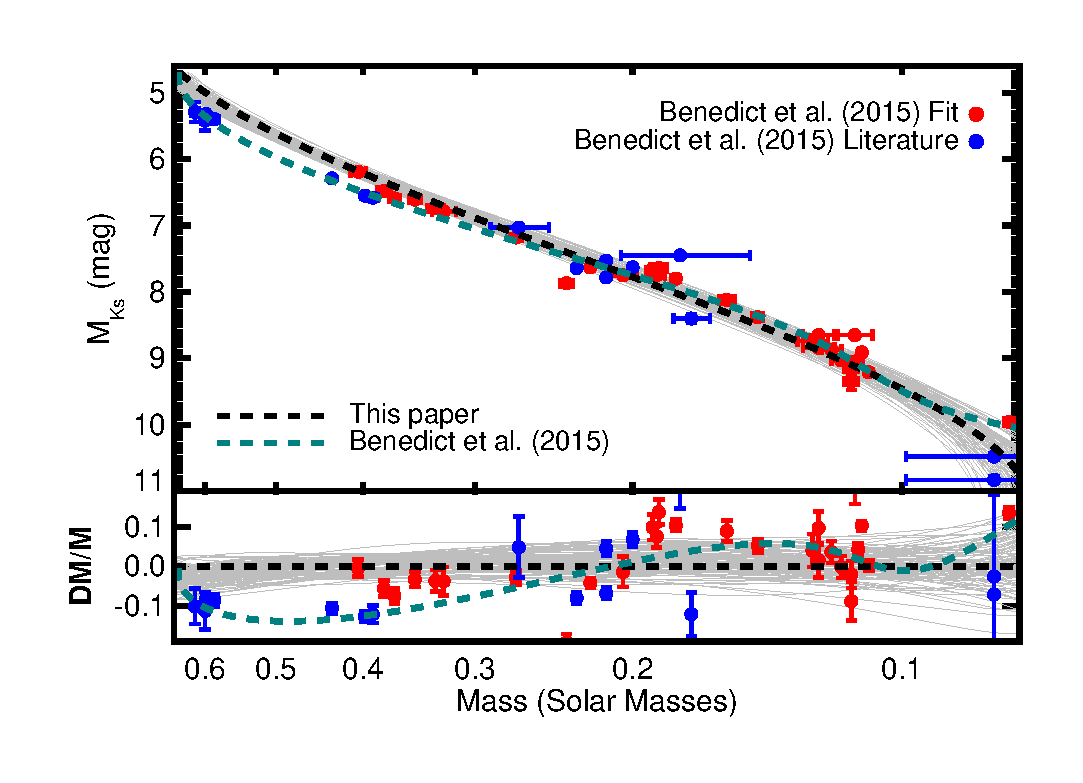
\includegraphics[width=0.47\textwidth]{Benedict_comp.eps}
\caption{Absolute $K_S$-band magnitude as a function of $M_*$ for astrometric binaries analyzed by \citet{Benedict2016} (red circles) and those used in the \citet{Benedict2016} relation, but pulled from the literature (blue circles). The resulting $M_*$-\mks\ relation from \citet{Benedict2016} is shown as a teal dashed line, while the best-fit relation from this paper is as a black dashed line (with random samplings in grey as in earlier figures). The bottom panel shows the residual of the \citet{Benedict2016} points compared to our relation, with the \citet{Benedict2016} relation in teal for reference. Errors in the residuals only reflect errors in $M_*$ and \mks, and do not account for errors in our $M_*$-\mks\ relation. }
\label{fig:benedict}
\end{center}
\end{figure}

%% problematic points:
%% GJ 278 C GJ 278 D (YY Gem): can't figure out where the K magnitudes came from?
%% GJ 570 B GJ 570 C: This is in our sample. We get total mass of 0.833�0.053, they get 0.976�0.012. They report delk~1.18, while we get 0.995. 
%% GJ 2069 A GJ 2069 C: Junky (bolometric correction) parallax and K 
%% GU Boo A GU Boo B: Crappy parallax and K

%\subsection{Testing mass ratio predictions}
%This test is a bit of a wash. There's broad agreement, but there's a few points that are way off. They are the same ones we mismatch on with Benedict. I think they are doing something funny with SB1s (not accounting for bias from the companion lines?). Can't quite tell from the paper. This is probably not worth the effort. 

%\subsection{Applications}
% This would be a section where we calculate the mass of a few more famous systems, e.g., Kepler-42, GJ1214, Trappist-1, etc. 
%I think this would be cool but the paper is SUPER long. 

\section{Conclusions \& Discussion}\label{sec:discussion} 

\subsection{Summary}
The mass-luminosity relation has proven to be a critical tool for estimating masses of cool stars for decades, and has applications from studying extrasolar planets to measuring the initial mass function and mass-to-light ratio in massive galaxies. The \mmk\ relation has been particularly useful because $K$-band magnitudes are widely available through 2MASS and other sources, extinction is usually negligible for nearby stars at these wavelengths, and there is minimal affect by metallicity. With the arrival of Gaia parallaxes combined with existing 2MASS photometry, nearly all the early M-dwarfs out to $\simeq$100\,pc and late M-dwarfs out to $\simeq$50\,pc have precise ($\lesssim1\%$) parallaxes and \mks\ magnitudes, massively increasing the utility of this relation. 

We endeavored to improve on existing \mmk\ relations and evaluate the role of [Fe/H] on the relation by expanding the sample of calibrators and using new techniques to measure the metallicity of binary M dwarfs. As part of this effort, we have been monitoring a set of nearby late K and M dwarf visual binaries using adaptive optics imaging with the goal of mapping their orbits and estimating their masses. We combined these data with similar data from Keck, CFHT, Gemini, and VLT archives, as well as astrometric measurements from the literature. The combination of literature astrometry and the recent Keck measurements were particularly important to provide the required baseline to fit long-period ($P>10$ years) orbits. 

We used these data to fit the orbits for 52 binaries, which we combined with parallaxes from the literature or derived from MEarth astrometry to determine the total masses of each system. We combined this with seven ultracool binaries from \citep{Dupuy2017}, which were analyzed in a nearly identical way to the procedure used in this paper and provide significantly improved coverage near the hydrogen burning limit. Seven binaries have total mass determinations better than 1\%, with a median precision of 6\%.

We used our dynamical masses and resolved \mks\ magnitudes to fit for an empirical relation between $M_*$ and \mks. The relation covers almost an order of magnitude in $M_*$, from $\simeq0.7M\odot$ down to the hydrogen burning limit ($\simeq0.075M_\odot$) and includes stars spanning the range of [Fe/H] expected for the Solar neighborhood ($-0.6<$[Fe/H]$<+0.4$).

The result provides masses precise to $\simeq$2\% over most of the M dwarf sequence. The uncertainty is limited primarily by scatter in the input masses around the best-fit above what is expected given their assigned mass uncertainties (median error on total $M_*$ of 5.6\%). We characterize this scatter with a free parameter ($\sigma_e$), which we find to be $\simeq$2\% for all fits. It is unclear if $\sigma_e$ arose from intrinsic variation in the \mmk\ relation due to a missing astrophysical parameter, such as age/activity/rotation \citep[e.g.,][]{Kraus2011,Feiden:2016aa,Somers2017} or detailed abundances \citep[e.g.,][]{2017A&A...604A..97L,Veyette2017}, or underestimated errors in the input masses. Our adopted parallaxes, in particular, could have their uncertainties underestimated due to uncorrected orbital motion in the input astrometry. Although this does not impact many of our systems, for which the parallax was drawn from a wide proper motion companion or accounting for orbital motion, enough of the sample could be impacted by this to explain much of the missing 2\%. 

Using empirically calibrated spectroscopic abundances, we explored the role of [Fe/H] on the \mmk\ relation, comparing our results to expectations from evolutionary models as a guide. While the MIST models follow our empirical data relatively well, they significantly overestimate the importance of [Fe/H] in the \mmk\ relation (4.0$\sigma$). This difference does not appear to be due to systematics in the [Fe/H] estimates and holds even when we only include targets with the most reliable masses and/or metallicities. Interestingly, the effect of [Fe/H] is consistent with zero at 1.7$\sigma$, suggesting a metallicity effect so weak that we will need to include targets with more extreme metallicities to characterize it. 

We compared our relation to recent similar relations in the literature. Given quoted uncertainties, both the \citet{Delfosse2000} and \citet{Mann2015b} relations follow ours well over most of the sequence. Since the \citet{Mann2015b} masses are rooted in an updated version of the DSEP code, the level of agreement suggests that these models perform extremely well in predicting the masses of old, main-sequence M dwarfs. 

Our results agreed well with the observational sample of astrometric binaries analyzed by \citet{Benedict2016}, but our relation diverges from \citet{Benedict2016} above $\simeq0.35M_\odot$. We attribute this difference to literature points included in the \citet{Benedict2016} fit from earlier analyses (mostly eclipsing binaries) with uncertain distances and $\Delta K_S$ magnitudes. Increasing availability of Gaia parallaxes for these systems as well as ongoing efforts to measure their eclipses in range of wavelengths \citep[e.g.,][]{2017AJ....154..100H} should significantly improve their utility for studying the mass-luminosity relation of M dwarfs.


\subsection{Suggestions when using our \mmk\ relation}\label{sec:caveats}

To help users interested in using \mks\ to compute a realistic $M_*$ and $\sigma_{M_*}$ of single stars with parallaxes and $K_S$ magnitudes, we provide \href{https://github.com/awmann/M_-M_K-}{a simple code} to sample the fit posterior. {\bf Before using that code or the provided MCMC posteriors, take note of the following suggestions:}
\begin{itemize}
\item The fit behaves poorly near the edges of the calibration sample. The scatter in the MCMC posterior accounts for this, but restrict use to $4.0<M_{K_S}<11.0$ ($0.075M_\odot<M_*<0.74M_\odot$), and a `safe' range would be $4.5<M_{K_S}<10.5$ ($0.08M_\odot<M_*<0.67M_\odot$). 

\item Our relation is only valid for main-sequence stars, and the roles of youth and activity are not accounted for here. Based on the Lyon models \citep{BHAC15}, we advise restricting use to $>$100\,Myr above $0.4M_\odot$, $>$300\,Myr to $0.2M_\odot$, $>$500\,Myr to $0.1M_\odot$, and $>1$\,Gyr below 0.1$M_\odot$. A safer cut would be to only use this on stars $>$1 Gyr, similar to the calibration sample. 

\item The sample metallicity spans $-0.60<\rm{[Fe/H]}<+0.45$, but 85\% of the binaries have $-0.40<\rm{[Fe/H]}<+0.30$. We provide a fit that attempts to take into account changes due to [Fe/H], but find a surprisingly weak effect. This suggests the [Fe/H]-free relation is safe to use over the range of metallicities expected in the Solar neighborhood (similar to the calibration sample). However, given the paucity of extreme metallicity systems in our calibration sample, we advise caution when targeting more metal-poor populations like the thick disk or halo ([Fe/H]$\ll-0.5$). The effects of more detailed abundances (e.g., [$\alpha$/Fe]) are completely untested.

\item The relation is only tested above the hydrogen burning limit. Since the boundary likely depends on metallicity \citep{2001RvMP...73..719B}, it is also not possible to use a simple $M_{K_S}$ cut even if the target is known to be old. Objects just below the hydrogen burning limit age slowly \citep{BHAC15}, so the relation given here may give reasonable results for many of these, but we urge caution when interpreting $M_*$ values for $M_{K_S}>10.5$. 

\item Since the origin of the $\sigma_e$ value is unclear, we suggest always including this as an irreducible source of error when estimating the mass of a target. 

\end{itemize}


\subsection{Future directions}

We intentionally selected targets that had $\Delta K$ measurements, as \mks\ was known to give the tightest relation with $M_*$ for M dwarfs. Unfortunately, there is no other band with contrast ratios for all systems considered here. Most of our monitoring was done with NIRC2 on Keck, so many systems have a $\Delta H$, but only about 1/3 of the sample have measurements in an optical band. This limits the utility of the sample, as Gaia $G$, $BP$, and $RP$ are now widely available for early and mid-M dwarfs, and are generally measured with better precision than 2MASS $K_S$. The growing capabilities of speckle cameras \citep[e.g.,][]{2009AJ....137.5057H} offer the opportunity to add optical contrasts. These can be converted to Gaia bandpasses, given reasonable assumptions about the component spectra, and used to derive a $M_{G}-M_*$ (or $M_G-M_*$-[Fe/H]) relation that can be easily applied to millions of K and M dwarfs. Complementary optical data also provide colors for individual components, from which we can measure component \teff\ and luminosity \citep[e.g.,][]{2017ApJ...845...72K}.

Our sample was limited mostly to stars in the Solar neighborhood, and hence was heavily biased towards the narrow [Fe/H] distribution of nearby stars. We identified five additional [Fe/H]$<-0.5$ systems including two subdwarf binaries. However all systems had short baselines in the literature compared to their expected orbital periods. It may take 1-2 more years to complete their orbits at the required precision for this kind of analysis. The availability of Gaia parallaxes will also help improve the precision of the known metal-poor systems and aid in the identification of new ones. Lastly, as new methods arrive to measure detailed abundances of M dwarfs \citep{Veyette2016a,Veyette2017} we can explore effects beyond just [Fe/H]. This is especially useful for systems with large enough radial velocity differences between component stars to separate out individual spectra at high resolution.


Although the sample studied here contained 118 stars, we only had half that many data points (59) constraining the fit, as the mass ratios were not known. This complicates the fit at the bottom of the sequence somewhat, where the relation is steeper. Here, small changes in the shape can have a larger impact on the implied mass ratio for a given system, providing a means to generate many reasonable solutions to the same set of system masses. This can be seen in Figure~\ref{fig:relation} as a spread in the range of possible solutions for \mks$>10$ despite relatively well-determined masses for these systems. Later Gaia data releases will include full astrometry information, which, when combined with a measure of the flux ratio and our existing astrometry will enable a global fit for individual masses as well as the system parallax. 

The presence of unresolved tight companions (triples or quadruples) could bias the overall relation. A close-in third star orbiting one of the two binary components might be stable, and would not have been detected in our AO data. An unresolved, less massive companion would drive the total mass of the system higher, but has a much smaller effect on the total luminosity. So unresolved triples will sit {\it low} in Figure~\ref{fig:relation} (higher mass for a fixed \mks). A few stars do sit well below the fit, but not more so than expected given their mass uncertainties. Many of our targets have some radial velocity data in the literature \citep[e.g.,][]{1999A&A...344..897D,Raghavan2010,Benedict2016}, which rule out the presence of any unresolved stellar companion. However, a more detailed analysis will require re-analysis of the radial velocity data to determine the maximum mass of an undetected companion for each individual system and convert that into a bias on the relation. 

Ages of our binary sample are not known, preventing any study into the effects of age on the \mmk\ relation. However, our larger sample of binaries with orbit measurements still in progress contains known members of nearby young moving groups and the Hyades cluster. Many of these have complete or nearly complete orbital solutions, and will soon provide a powerful set of mass benchmarks with known ages. These systems span ages from 10-650\,Myr, offering the chance to both test pre-main-sequence models of M dwarfs \citep{2015ApJ...813L..11M,2016ApJ...817..164R,2016ApJ...818..156C,2016AJ....152..175N} and explore the role of activity on M dwarf parameters \citep[e.g.,][]{Spada2013,2018arXiv180404133K}. The current sample can be included in such work when combined with age indicators like kinematics \citep{2018MNRAS.tmp..966W}, ultraviolet flux \citep{Ansdell2015}, and rotation periods expected from the Transiting Exoplanet Survey Satellite \citep[{\it TESS},][]{2014SPIE.9143E..20R}. 


\acknowledgements
AWM was supported through Hubble Fellowship grant 51364 awarded by the Space Telescope Science Institute, which is operated by the Association of Universities for Research in Astronomy, Inc., for NASA, under contract NAS 5-26555. This work was supported by a NASA Keck PI Data Award (award numbers 1554237, 1544189, 1535910, and 1521162), administered by the NASA Exoplanet Science Institute. Data presented herein were obtained at the W. M. Keck Observatory from telescope time allocated to the National Aeronautics and Space Administration through the agency's scientific partnership with the California Institute of Technology and the University of California. The Observatory was made possible by the generous financial support of the W. M. Keck Foundation.

The authors wish to recognize and acknowledge the very significant cultural role and reverence that the summit of Mauna Kea has always had within the indigenous Hawaiian community. We are most fortunate to have the opportunity to conduct observations from this mountain.

The authors acknowledge the Texas Advanced Computing Center (TACC) at The University of Texas at Austin for providing grid resources that have contributed to the research results reported within this paper. URL: http://www.tacc.utexas.edu.

Based on observations obtained at the Gemini Observatory (acquired through the Gemini Observatory Archive), which is operated by the Association of Universities for Research in Astronomy, Inc., under a cooperative agreement with the NSF on behalf of the Gemini partnership: the National Science Foundation (United States), the National Research Council (Canada), CONICYT (Chile), Ministerio de Ciencia, Tecnolog\'{i}a e Innovaci\'{o}n Productiva (Argentina), and Minist\'{e}rio da Ci\^{e}ncia, Tecnologia e Inova\c{c}\~{a}o (Brazil). Observations taken from programs GN-2008B-Q-57, GN-2009B-Q-10, GN-2010B-Q-9, and GN-2011A-Q-26.

Based on observations collected at the European Organisation for Astronomical Research in the Southern Hemisphere under ESO programmes 071.C-0388(A), 072.C-0570(A), 073.C-0155(A), 075.C-0521(A), 075.C-0733(A), 077.C-0783(A), 078.C-0441(A), 079.C-0216(A), 080.C-0424(A), 081.C-0430(A), 082.C-0518(A), 082.C-0518(B), 085.C-0867(B), 086.C-0515(A), 086.C-0515(B), 090.C-0448(A), 091.D-0804(A), 098.C-0597(A), 382.C-0324(A), and 382.D-0754(A).

 This research has made use of the Keck Observatory Archive (KOA), which is operated by the W. M. Keck Observatory and the NASA Exoplanet Science Institute (NExScI), under contract with the National Aeronautics and Space Administration. 

Based on observations obtained at the Canada-France-Hawaii Telescope (CFHT) which is operated by the National Research Council of Canada, the Institut National des Sciences de l'Univers of the Centre National de la Recherche Scientifique of France, and the University of Hawaii. 

This work presents results from the European Space Agency (ESA) space mission Gaia. Gaia data are being processed by the Gaia Data Processing and Analysis Consortium (DPAC). Funding for the DPAC is provided by national institutions, in particular the institutions participating in the Gaia MultiLateral Agreement (MLA). The Gaia mission website is \href{https://www.cosmos.esa.int/gaia}{https://www.cosmos.esa.int/gaia}. The Gaia archive website is \href{https://archives.esac.esa.int/gaia}{https://archives.esac.esa.int/gaia}.

\software{emcee, corner.py, mpfit, scipy, pyfits, astropy, python, spextools, IDL}

\facilities{Keck:II (NIRC2), IRTF (SpeX), CFHT (PUEO, aobir), VLT:Antu (NaCo); Gemini:North (NIRI)}

\bibliography{$HOME/Dropbox/fullbiblio}


\startlongtable
\begin{deluxetable*}{l l l l l l l l l l l l l l l l l l l l l l l }
\tablewidth{\linewidth}
\tablecaption{Binary Sample \label{tab:sample}}
\tablehead{
    \colhead{Name} & \colhead{Comp} & \colhead{R.A.} & \colhead{Dec} & \colhead{System $K_S$} 
 & \colhead{$\Delta K_S$} & \colhead{$M_{\rm tot}$} & \colhead{[Fe/H]$^a$} & \colhead{Plx}  & \colhead{Plx} \\
    \colhead{} & \colhead{} & \colhead{J2000} & \colhead{J2000} & \colhead{(mag)}
 & \colhead{(mag)} & \colhead{($M_\odot$)} & \colhead{(dex)} & \colhead{(mas)} & \colhead{Ref} 
}
\startdata
\multicolumn{10}{c}{Systems analyzed in this paper}  \\
\hline
GJ 1005 & AB & 00:15:28.0 & $-$16:08:01 & \phantom{0} 6.310$\pm$0.018$^b$ &  1.145$\pm$0.016 & 0.319$\pm$0.002 & $-$0.41 & 166.60\phantom{0}$\pm$0.30 & 3\\
GJ 2005 & BC & 00:24:44.1 & $-$27:08:24 & \phantom{0} 9.371$\pm$0.050$^e$ &  0.320$\pm$0.016 & 0.157$\pm$0.006 & $-$0.08 &  128.5\phantom{00}$\pm$1.5 & 3\\
Gl 22 & AC & 00:32:29.2 & $+$67:14:08 & \phantom{0} 6.037$\pm$0.023 &  2.060$\pm$0.035 & 0.548$\pm$0.003 & $-$0.24 & 100.405$\pm$0.070 & 3\\
Gl 54 & AB & 01:10:22.8 & $-$67:26:42 & \phantom{0} 5.132$\pm$0.024 &  0.697$\pm$0.036 & 0.750$\pm$0.010 & $+$0.17 & 126.90\phantom{0}$\pm$0.40 & 3\\
GJ 1038 & AB & 01:25:01.8 & $-$32:51:04 & \phantom{0} 6.207$\pm$0.021 &  0.058$\pm$0.016 & 1.301$\pm$0.204 & $+$0.03 & \phantom{0}39.8\phantom{00}$\pm$1.6 & 2\\
Gl 65 & AB & 01:39:01.2 & $-$17:57:02 & \phantom{0} 5.343$\pm$0.021 &  0.161$\pm$0.019 & 0.237$\pm$0.005 & $+$0.04 &  373.7\phantom{00}$\pm$2.7 & 5\\
Gl 84 & AB & 02:05:04.8 & $-$17:36:52 & \phantom{0} 5.662$\pm$0.020 &  3.262$\pm$0.016 & 0.517$\pm$0.028 & $-$0.14 &  109.4\phantom{00}$\pm$1.9 & 2,5\\
2M0213+36 & AB & 02:13:20.6 & $+$36:48:50 & \phantom{0} 8.518$\pm$0.018 &  1.493$\pm$0.018 & 0.245$\pm$0.035 & $-$0.07 & \phantom{0}74.6\phantom{00}$\pm$3.5 & 6\\
Gl 98 & AB & 02:27:45.9 & $+$04:25:55 & \phantom{0} 5.113$\pm$0.018 &  0.068$\pm$0.015 & 1.389$\pm$0.079 & $+$0.41 & \phantom{0}58.3\phantom{00}$\pm$1.1 & 2\\
Gl 99 & AB & 02:28:46.5 & $+$32:15:34 & \phantom{0} 6.062$\pm$0.018 &  0.254$\pm$0.016 & 1.457$\pm$0.183 & $+$0.21 & \phantom{0}38.2\phantom{00}$\pm$1.6 & 2\\
Gl 125 & AB & 03:09:30.8 & $+$45:43:58 & \phantom{0} 5.840$\pm$0.016 &  1.140$\pm$0.016 & 0.905$\pm$0.081 & $+$0.49 & \phantom{0}63.5\phantom{00}$\pm$1.9 & 2\\
Gl 190 & AB & 05:08:35.0 & $-$18:10:18 & \phantom{0} 5.314$\pm$0.018 &  0.103$\pm$0.017 & 0.835$\pm$0.053 & $+$0.25 &  107.9\phantom{00}$\pm$2.1 & 2\\
GJ 1081 & AB & 05:33:19.1 & $+$44:48:58 & \phantom{0} 7.335$\pm$0.027 &  0.949$\pm$0.018 & 0.583$\pm$0.043 & $-$0.03 & \phantom{0}65.20\phantom{0}$\pm$0.40 & 3\\
Gl 234 & AB & 06:29:23.3 & $-$02:48:49 & \phantom{0} 5.421$\pm$0.018$^b$ &  1.526$\pm$0.016 & 0.333$\pm$0.002 & $+$0.11 & 241.00\phantom{0}$\pm$0.40 & 3\\
GJ 3412 & AB & 06:54:04.2 & $+$60:52:18 & \phantom{0} 6.391$\pm$0.025$^b$ &  1.120$\pm$0.016 & 0.528$\pm$0.007 & $-$0.21 & \phantom{0}95.60\phantom{0}$\pm$0.30 & 3\\
GJ 3421 & AB & 07:03:55.7 & $+$52:42:06 & \phantom{0} 7.776$\pm$0.021 &  0.155$\pm$0.017 & 0.248$\pm$0.009 & $-$0.60 &  112.6\phantom{00}$\pm$1.4 & 3\\
Gl 263 & AB & 07:04:17.7 & $-$10:30:31 & \phantom{0} 6.427$\pm$0.017 &  0.441$\pm$0.020 & 0.951$\pm$0.141 & $+$0.43 & \phantom{0}62.0\phantom{00}$\pm$2.9 & 2,5\\
Gl 277 & AC & 07:31:57.7 & $+$36:13:09 & \phantom{0} 5.927$\pm$0.017 &  1.931$\pm$0.016 & 0.738$\pm$0.020 & $+$0.18 & \phantom{0}83.330$\pm$0.070 & 12\\
GJ 3454 & AB & 07:36:25.1 & $+$07:04:43 & \phantom{0} 7.282$\pm$0.020 &  0.272$\pm$0.016 & 0.279$\pm$0.015 & $+$0.03 &  117.1\phantom{00}$\pm$2.1 & 1\\
Gl 301 & AB & 08:13:08.5 & $-$13:55:01 & \phantom{0} 5.815$\pm$0.026 &  0.506$\pm$0.018 & 1.227$\pm$0.144 & $-$0.18 & \phantom{0}52.1\phantom{00}$\pm$2.0 & 5,8\\
Gl 310 & AB & 08:36:25.5 & $+$67:17:42 & \phantom{0} 5.580$\pm$0.015 &  2.134$\pm$0.017 & 0.778$\pm$0.067 & $-$0.06 & \phantom{0}72.6\phantom{00}$\pm$1.3 & 2\\
Gl 330 & AB & 08:57:04.6 & $+$11:38:49 & \phantom{0} 6.486$\pm$0.023 &  1.086$\pm$0.016 & 0.915$\pm$0.142 & $-$0.17 & \phantom{0}58.8\phantom{00}$\pm$2.7 & 2\\
LHS 6167 & AB & 09:15:36.4 & $-$10:35:47 & \phantom{0} 7.733$\pm$0.017 &  0.143$\pm$0.016 & 0.281$\pm$0.009 & $-$0.13 &  103.3\phantom{00}$\pm$1.0 & 10\\
Gl 340 & AB & 09:17:53.4 & $+$28:33:38 & \phantom{0} 4.767$\pm$0.017 &  0.024$\pm$0.020 & 1.357$\pm$0.055 & $-$0.39 & \phantom{0}57.92\phantom{0}$\pm$0.76 & 2\\
Gl 352 & AB & 09:31:19.4 & $-$13:29:19 & \phantom{0} 5.511$\pm$0.020 &  0.119$\pm$0.018 & 0.780$\pm$0.075 & $-$0.03 & \phantom{0}98.5\phantom{00}$\pm$3.1 & 5,9\\
Gl 381 & AB & 10:12:04.6 & $-$02:41:04 & \phantom{0} 6.193$\pm$0.026 &  0.811$\pm$0.016 & 0.765$\pm$0.082 & $-$0.12 & \phantom{0}83.5\phantom{00}$\pm$2.8 & 2,5\\
Gl 416 & AB & 11:11:33.1 & $-$14:59:28 & \phantom{0} 5.874$\pm$0.017 &  0.980$\pm$0.017 & 1.192$\pm$0.102 & $-$0.20 & \phantom{0}46.4\phantom{00}$\pm$1.3 & 2\\
Gl 469 & AB & 12:28:57.6 & $+$08:25:31 & \phantom{0} 6.956$\pm$0.026 &  1.100$\pm$0.016 & 0.514$\pm$0.011 & $+$0.19 & \phantom{0}76.40\phantom{0}$\pm$0.50 & 3\\
Gl 473 & AB & 12:33:17.4 & $+$09:01:15 & \phantom{0} 6.042$\pm$0.020 &  0.001$\pm$0.018 & 0.262$\pm$0.016 & $+$0.09 &  227.9\phantom{00}$\pm$4.6 & 5\\
Gl 494 & AB & 13:00:46.6 & $+$12:22:32 & \phantom{0} 5.578$\pm$0.016 &  4.269$\pm$0.017 & 0.667$\pm$0.035 & $+$0.30 & \phantom{0}85.5\phantom{00}$\pm$1.5 & 2\\
Gl 570 & BC & 14:57:26.5 & $-$21:24:40 & \phantom{0} 3.855$\pm$0.045$^b$ &  0.995$\pm$0.046 & 0.837$\pm$0.052 & $+$0.18 & 171.22\phantom{0}$\pm$0.94 & 2\\
Gl 600 & AB & 15:52:08.1 & $+$10:52:28 & \phantom{0} 5.819$\pm$0.023 &  0.029$\pm$0.018 & 1.228$\pm$0.032 & $+$0.01 & \phantom{0}47.65\phantom{0}$\pm$0.30 & 11\\
Gl 623 & AB & 16:24:09.2 & $+$48:21:10 & \phantom{0} 5.915$\pm$0.023 &  2.501$\pm$0.040 & 0.465$\pm$0.004 & $-$0.44 & 127.50\phantom{0}$\pm$0.30 & 3\\
GJ 1210 & AB & 17:07:40.8 & $+$07:22:06 & \phantom{0} 8.419$\pm$0.025 &  0.075$\pm$0.017 & 0.218$\pm$0.019 & $-$0.19 & \phantom{0}86.8\phantom{00}$\pm$2.5 & 1\\
Gl 660 & AB & 17:11:52.2 & $-$01:51:06 & \phantom{0} 6.656$\pm$0.021 &  0.033$\pm$0.017 & 0.606$\pm$0.053 & $-$0.20 & \phantom{0}85.2\phantom{00}$\pm$2.5 & 5,9\\
Gl 661 & AB & 17:12:07.8 & $+$45:39:58 & \phantom{0} 4.834$\pm$0.023 &  0.251$\pm$0.020 & 0.596$\pm$0.054 & $-$0.41 &  167.3\phantom{00}$\pm$5.0 & 2\\
GJ 4024 & AB & 17:43:00.7 & $+$05:47:21 & \phantom{0} 6.631$\pm$0.018 &  0.931$\pm$0.016 & 0.917$\pm$0.139 & $-$0.09 & \phantom{0}50.1\phantom{00}$\pm$2.5 & 2\\
Gl 695 & BC & 17:46:25.1 & $+$27:43:00 & \phantom{0} 4.953$\pm$0.016 &  0.287$\pm$0.016 & 0.868$\pm$0.023 & $+$0.22 & 120.33\phantom{0}$\pm$0.16 & 2\\
Gl 747 & AB & 19:07:42.9 & $+$32:32:41 & \phantom{0} 6.416$\pm$0.020 &  0.098$\pm$0.016 & 0.429$\pm$0.026 & $-$0.20 &  122.3\phantom{00}$\pm$2.5 & 5\\
Gl 748 & AB & 19:12:14.5 & $+$02:53:11 & \phantom{0} 6.342$\pm$0.018$^b$ &  1.035$\pm$0.024 & 0.538$\pm$0.007 & $-$0.23 & \phantom{0}98.40\phantom{0}$\pm$0.30 & 3\\
Gl 762.1 & AB & 19:31:08.5 & $+$58:35:13 & \phantom{0} 4.463$\pm$0.015 &  0.080$\pm$0.121 & 1.469$\pm$0.067 & $-$0.17 & \phantom{0}58.37\phantom{0}$\pm$0.54 & 2\\
Gl 765.2 & AB & 19:39:05.9 & $+$76:25:18 & \phantom{0} 5.898$\pm$0.016 &  0.371$\pm$0.037 & 1.330$\pm$0.068 & $-$0.35 & \phantom{0}33.67\phantom{0}$\pm$0.53 & 2\\
GJ 1245 & AC & 19:53:54.4 & $+$44:24:53 & \phantom{0} 6.854$\pm$0.016 &  1.124$\pm$0.016 & 0.203$\pm$0.000 & $+$0.01 & 214.528$\pm$0.082 & 12\\
Gl 791.2 & AB & 20:29:48.3 & $+$09:41:20 & \phantom{0} 7.307$\pm$0.024 &  1.565$\pm$0.018 & 0.298$\pm$0.020 & $+$0.05 & 113.40\phantom{0}$\pm$0.20 & 3\\
Gl 804 & AB & 20:44:21.9 & $+$19:44:59 & \phantom{0} 6.553$\pm$0.016 &  1.083$\pm$0.016 & 0.996$\pm$0.135 & $-$0.09 & \phantom{0}47.4\phantom{00}$\pm$2.1 & 2\\
Gl 831 & AB & 21:31:18.5 & $-$09:47:26 & \phantom{0} 6.379$\pm$0.020 &  1.221$\pm$0.016 & 0.418$\pm$0.003 & $+$0.20 & 125.30\phantom{0}$\pm$0.30 & 3\\
Gl 844 & AB & 22:01:49.0 & $+$16:28:02 & \phantom{0} 6.180$\pm$0.021 &  0.108$\pm$0.016 & 0.872$\pm$0.095 & $+$0.21 & \phantom{0}61.8\phantom{00}$\pm$2.2 & 2\\
HD 239960 & AB & 22:27:59.5 & $+$57:41:45 & \phantom{0} 4.777$\pm$0.029 &  0.994$\pm$0.017 & 0.460$\pm$0.011 & $-$0.11 &  249.9\phantom{00}$\pm$1.9 & 2\\
GJ4287 & AB & 22:37:29.9 & $+$39:22:51 & \phantom{0} 5.872$\pm$0.027 &  0.913$\pm$0.016 & 1.187$\pm$0.020 & $+$0.03 & \phantom{0}47.61\phantom{0}$\pm$0.20 & 12\\
Gl 893.4 & AB & 23:16:39.7 & $+$19:37:17 & \phantom{0} 7.303$\pm$0.017 &  0.052$\pm$0.016 & 0.846$\pm$0.117 & $-$0.17 & \phantom{0}32.5\phantom{00}$\pm$1.5 & 1\\
Gl 900 & BC & 23:35:00.2 & $+$01:36:19 & \phantom{0} 7.571$\pm$0.050$^e$ &  0.758$\pm$0.018 & 0.610$\pm$0.016 & $+$0.03 & \phantom{0}48.17\phantom{0}$\pm$0.31 & 11\\
Gl 913 & AB & 23:58:43.4 & $+$46:43:44 & \phantom{0} 5.831$\pm$0.020 &  1.327$\pm$0.018 & 0.890$\pm$0.118 & $-$0.12 & \phantom{0}68.0\phantom{00}$\pm$3.0 & 7\\
\hline
\multicolumn{10}{c}{Systems from \citet{Dupuy2017} }  \\
\hline
LHS1901 & AB & 07:11:11.4 & $+$43:29:58 & \phantom{0} 9.126$\pm$0.018 &  0.094$\pm$0.010 & 0.203$\pm$0.009 & $-$0.41 & \phantom{0}76.4\phantom{00}$\pm$1.1 & 4\\
2M0746+20 & AB & 07:46:42.5 & $+$20:00:32 & \phantom{0}10.468$\pm$0.022 &  0.357$\pm$0.025 & 0.154$\pm$0.002 & $-$0.18$^d$ & \phantom{0}81.24\phantom{0}$\pm$0.25 & 4\\
2M1017+13 & AB & 10:17:07.5 & $+$13:08:39 & \phantom{0}12.710$\pm$0.023 &  0.113$\pm$0.024 & 0.149$\pm$0.016 & $-$0.35$^d$ & \phantom{0}32.2\phantom{00}$\pm$1.2 & 4\\
2M1047+40 & AB & 10:47:13.8 & $+$40:26:49 & \phantom{0}11.254$\pm$0.018 &  0.289$\pm$0.049 & 0.171$\pm$0.012 & $+$0.17 & \phantom{0}39.02\phantom{0}$\pm$0.90 & 4\\
LSJ1735+26 & AB & 17:35:12.9 & $+$26:34:47 & \phantom{0}10.157$\pm$0.020 &  0.490$\pm$0.020 & 0.178$\pm$0.008 & $+$0.03 & \phantom{0}64.82\phantom{0}$\pm$0.95 & 4\\
2M2140+16 & AB & 21:40:29.3 & $+$16:25:18 & \phantom{0}11.826$\pm$0.031 &  0.743$\pm$0.075 & 0.190$\pm$0.017 & $-$0.10$^c$ & \phantom{0}29.52\phantom{0}$\pm$0.88 & 4\\
2M2206-20 & AB & 22:06:22.8 & $-$20:47:05 & \phantom{0}11.315$\pm$0.027 &  0.067$\pm$0.016 & 0.168$\pm$0.016 & $-$0.05$^c$ & \phantom{0}36.6\phantom{00}$\pm$1.2 & 4\\
\enddata
\tablecomments{Parallax references: 1 = This work (MEarth), 2 = \citet{van-Leeuwen:2007yq}, 3 = \citet{Benedict2016}, 4 = \citet{Dupuy2017}, 5 = \citet{van-Altena1995}, 6 = \citet{2016AJ....151..160F}, 7 = \citet{2006ApJS..166..341G}, 8 = \citet{Winters2015}, 9 = \citet{Soderhjelm1999}, 10 = \citet{2017AJ....154..151B}, 11 = \citet{gaiadr1}, 12 = companion to star in \citet{GaiaDr2}.}
\tablenotetext{$a$}{Errors on [Fe/H] are limited primarily by the calibration \citep{Mann2013a,Mann2014}, and are 0.08~dex for all targets unless otherwise noted. }
\tablenotetext{$b$}{Synthetic $K_S$ magnitudes derived from spectra. All other $K_S$ magnitudes are from 2MASS. }
\tablenotetext{$c$}{Abundance derived from lower-resolution IRTF spectrum, $\sigma$[Fe/H] estimated to be 0.12~dex. }
\tablenotetext{$d$}{L dwarfs are beyond the calibration range of \citet{Mann2014} ; [Fe/H] values should be used with caution. }
\tablenotetext{$e$}{$K_S$ magnitude from 2MASS contains a third star, listed $K_S$ magnitude has third star's flux removed. }
\end{deluxetable*}


\begin{longrotatetable}
\begin{deluxetable*}{l l l l l l l l l r r}
\tablewidth{\linewidth}
\tablecaption{Orbital Parameters \label{tab:orbits}
}
\tablehead{
    \colhead{Name} & \colhead{$P$} & \colhead{$\alpha_{\rm{ang}}$} & \colhead{$e$} & \colhead{$i$} 
 & \colhead{$\omega$} & \colhead{$\Omega$} & \colhead{$T_0$} & \colhead{$\alpha_{\rm{ang}}^3/P^2$} & \colhead{$\chi^2$/dof} \\%& \colhead{dof} \\
    \colhead{} & \colhead{(years)} & \colhead{(mas)} & \colhead{} & \colhead{(degrees)}
 & \colhead{(degrees)} & \colhead{(degrees)} & \colhead{MJD} & \colhead{arcsec$^3\,yr^{-2}$} & \colhead{} %& \colhead{}
}
\startdata
GJ 1005 & \phantom{0}4.55726$^{+0.00075}_{-0.00074}$ & \phantom{0}312.85$^{+0.50}_{-0.50}$ & 0.36136$^{+0.00097}_{-0.00098}$ & 143.93$^{+0.25}_{-0.24}$ & 345.26$^{+0.62}_{-0.62}$ & \phantom{0}61.23$^{+0.41}_{-0.41}$ & 58172.9$^{+1.9}_{-1.9}$ & (1.4743$\pm$0.0072)x$10^3$ & 85.9/67\\
GJ 2005 & 17.296$^{+0.011}_{-0.011}$ & \phantom{0}463.36$^{+0.57}_{-0.56}$ & 0.02900$^{+0.00093}_{-0.00091}$ & \phantom{0}62.816$^{+0.050}_{-0.051}$ & 143.3$^{+2.4}_{-2.2}$ & \phantom{0}11.798$^{+0.084}_{-0.085}$ & 59158$^{+42}_{-40}$ & (3.326$\pm$0.015)x$10^4$ & 101.6/85\\
Gl 22 & 15.4275$^{+0.0054}_{-0.0054}$ & \phantom{0}510.26$^{+0.74}_{-0.74}$ & 0.1576$^{+0.0013}_{-0.0013}$ & \phantom{0}44.29$^{+0.15}_{-0.15}$ & 104.90$^{+0.53}_{-0.53}$ & 176.75$^{+0.21}_{-0.21}$ & 57447.0$^{+5.1}_{-5.2}$ & (5.582$\pm$0.026)x$10^4$ & 75.5/65\\
Gl 54 & \phantom{0}1.14434$^{+0.00022}_{-0.00022}$ & \phantom{0}126.19$^{+0.39}_{-0.39}$ & 0.1718$^{+0.0024}_{-0.0024}$ & 125.32$^{+0.35}_{-0.35}$ & \phantom{0}47.33$^{+0.92}_{-0.93}$ & \phantom{0}92.04$^{+0.40}_{-0.40}$ & 58124.0$^{+1.1}_{-1.1}$ & (1.534$\pm$0.014)x$10^3$ & 37.9/33\\
GJ 1038 & \phantom{0}5.98$^{+1.02}_{-0.77}$ & \phantom{0}139.7$^{+14.5}_{-9.7}$ & 0.54$^{+0.12}_{-0.11}$ & \phantom{0}72.9$^{+1.9}_{-2.5}$ & 174$^{+13}_{-16}$ & 105.9$^{+1.6}_{-2.7}$ & 58313$^{+41}_{-1976}$ & (7.67$\pm$0.52)x$10^5$ & 1.5/9\\
Gl 65 & 26.359$^{+0.025}_{-0.024}$ & 2049.6$^{+3.4}_{-3.4}$ & 0.6222$^{+0.0015}_{-0.0015}$ & 128.09$^{+0.15}_{-0.15}$ & 283.340$^{+0.085}_{-0.084}$ & 146.29$^{+0.14}_{-0.14}$ & 60591.9$^{+9.4}_{-9.4}$ & (1.2391$\pm$0.0058)x$10^2$ & 96.7/89\\
Gl 84 & 13.328$^{+0.037}_{-0.037}$ & \phantom{0}495.5$^{+1.2}_{-1.2}$ & 0.3771$^{+0.0082}_{-0.0081}$ & \phantom{0}91.771$^{+0.056}_{-0.057}$ & 245.62$^{+0.48}_{-0.48}$ & 102.987$^{+0.022}_{-0.022}$ & 61554$^{+14}_{-14}$ & (6.850$\pm$0.066)x$10^4$ & 21.4/17\\
2M0213+36 & \phantom{0}6.419$^{+0.067}_{-0.071}$ & \phantom{0}161.5$^{+1.3}_{-1.3}$ & 0.4232$^{+0.0039}_{-0.0038}$ & 115.30$^{+0.24}_{-0.24}$ & 207.66$^{+0.72}_{-0.73}$ & \phantom{0}83.73$^{+0.32}_{-0.33}$ & 57604.5$^{+2.8}_{-2.9}$ & (1.023$\pm$0.016)x$10^4$ & 28.8/11\\
Gl 98 & 25.255$^{+0.021}_{-0.021}$ & \phantom{0}559.84$^{+0.66}_{-0.65}$ & 0.2354$^{+0.0013}_{-0.0013}$ & \phantom{0}73.389$^{+0.048}_{-0.047}$ & 231.49$^{+0.21}_{-0.21}$ & 109.116$^{+0.022}_{-0.022}$ & 56417.3$^{+4.6}_{-4.7}$ & (2.7509$\pm$0.0098)x$10^4$ & 87.6/85\\
Gl 99 & 24.015$^{+0.086}_{-0.084}$ & \phantom{0}360.53$^{+0.72}_{-0.71}$ & 0.2087$^{+0.0028}_{-0.0025}$ & \phantom{0}84.605$^{+0.049}_{-0.049}$ & 152.6$^{+1.9}_{-1.9}$ & \phantom{0}98.836$^{+0.087}_{-0.090}$ & 56340$^{+43}_{-43}$ & (8.126$\pm$0.027)x$10^5$ & 23.8/25\\
Gl 125 & 25.67$^{+0.20}_{-0.19}$ & \phantom{0}534.5$^{+2.3}_{-2.3}$ & 0.2271$^{+0.0044}_{-0.0044}$ & \phantom{0}97.186$^{+0.026}_{-0.026}$ & 181.38$^{+0.35}_{-0.36}$ & \phantom{0}13.732$^{+0.082}_{-0.081}$ & 64226$^{+74}_{-73}$ & (2.3173$\pm$0.0098)x$10^4$ & 12.6/23\\
Gl 150.2 & 13.604$^{+0.045}_{-0.046}$ & \phantom{0}254.9$^{+1.3}_{-1.3}$ & 0.268$^{+0.011}_{-0.010}$ & 101.79$^{+0.38}_{-0.38}$ & 250.5$^{+1.2}_{-1.3}$ & 100.68$^{+0.46}_{-0.45}$ & 58570$^{+23}_{-24}$ & (8.95$\pm$0.16)x$10^5$ & 25.4/19\\
Gl 190 & \phantom{0}0.96380$^{+0.00024}_{-0.00024}$ & \phantom{00}99.12$^{+0.85}_{-0.85}$ & 0.2441$^{+0.0093}_{-0.0091}$ & \phantom{0}92.96$^{+0.26}_{-0.25}$ & 186.4$^{+5.7}_{-5.9}$ & \phantom{0}40.42$^{+0.17}_{-0.17}$ & 58182.4$^{+6.5}_{-6.7}$ & (1.048$\pm$0.027)x$10^3$ & 25.5/31\\
GJ 1081 & 11.593$^{+0.034}_{-0.033}$ & \phantom{0}272.9$^{+6.8}_{-6.1}$ & 0.8612$^{+0.0058}_{-0.0055}$ & \phantom{0}97.23$^{+0.35}_{-0.34}$ & 230.5$^{+1.5}_{-1.4}$ & \phantom{0}51.11$^{+0.14}_{-0.14}$ & 57220$^{+18}_{-17}$ & (1.51$\pm$0.10)x$10^4$ & 25.4/19\\
Gl 234 & 16.5777$^{+0.0027}_{-0.0027}$ & 1086.04$^{+0.27}_{-0.28}$ & 0.38229$^{+0.00013}_{-0.00013}$ & \phantom{0}52.910$^{+0.016}_{-0.016}$ & 220.942$^{+0.020}_{-0.020}$ & \phantom{0}30.385$^{+0.030}_{-0.030}$ & 57342.99$^{+0.23}_{-0.23}$ & (4.6612$\pm$0.0033)x$10^3$ & 123.2/105\\
LHS 221 & 13.5943$^{+0.0062}_{-0.0061}$ & \phantom{0}440.9$^{+1.6}_{-1.6}$ & 0.4777$^{+0.0022}_{-0.0022}$ & 109.76$^{+0.13}_{-0.13}$ & \phantom{0}58.59$^{+0.21}_{-0.21}$ & 107.20$^{+0.21}_{-0.21}$ & 59671.2$^{+2.5}_{-2.5}$ & (4.637$\pm$0.053)x$10^4$ & 30.5/49\\
LHS 224 & \phantom{0}3.2860$^{+0.0014}_{-0.0014}$ & \phantom{0}156.38$^{+0.29}_{-0.28}$ & 0.2231$^{+0.0045}_{-0.0044}$ & 131.76$^{+0.52}_{-0.53}$ & \phantom{0}73.73$^{+0.43}_{-0.43}$ & 173.93$^{+0.81}_{-0.84}$ & 58535.0$^{+4.9}_{-4.8}$ & (3.541$\pm$0.020)x$10^4$ & 19.2/27\\
Gl 263 & \phantom{0}3.6205$^{+0.0021}_{-0.0021}$ & \phantom{0}143.8$^{+2.1}_{-2.0}$ & 0.7158$^{+0.0065}_{-0.0064}$ & 103.28$^{+0.36}_{-0.36}$ & 287.52$^{+0.51}_{-0.51}$ & \phantom{0}81.04$^{+0.24}_{-0.24}$ & 58416.0$^{+3.6}_{-3.6}$ & (2.268$\pm$0.099)x$10^4$ & 21.9/17\\
Gl 277 & 53.0$^{+9.2}_{-7.2}$ & 1058$^{+113}_{-84}$ & 0.48$^{+0.14}_{-0.12}$ & \phantom{0}93.53$^{+0.48}_{-0.34}$ & \phantom{0}22$^{+332}_{-17}$ & \phantom{0}10.22$^{+0.26}_{-0.44}$ & 71033$^{+12032}_{-3397}$ & (4.22$\pm$0.16)x$10^4$ & 15.2/13\\
2M0736+07 & 23.768$^{+0.048}_{-0.046}$ & \phantom{0}633.29$^{+0.94}_{-0.93}$ & 0.58621$^{+0.00060}_{-0.00060}$ & \phantom{0}12.3$^{+1.0}_{-1.1}$ & \phantom{0}66.7$^{+5.6}_{-5.3}$ & \phantom{0}77.3$^{+4.9}_{-5.2}$ & 57466.3$^{+2.7}_{-2.7}$ & (4.495$\pm$0.019)x$10^4$ & 16.8/21\\
Gl 301 & 62.2$^{+1.8}_{-1.7}$ & \phantom{0}875$^{+10}_{-10}$ & 0.6778$^{+0.0049}_{-0.0048}$ & \phantom{0}52.31$^{+0.86}_{-0.87}$ & 167.4$^{+1.1}_{-1.1}$ & 142.0$^{+1.1}_{-1.1}$ & 51189$^{+18}_{-19}$ & (1.737$\pm$0.049)x$10^4$ & 20.1/13\\
Gl 310 & 23.48$^{+0.14}_{-0.14}$ & \phantom{0}552.6$^{+5.6}_{-5.4}$ & 0.6976$^{+0.0073}_{-0.0074}$ & 122.06$^{+0.57}_{-0.56}$ & 246.72$^{+0.36}_{-0.37}$ & \phantom{0}49.62$^{+0.39}_{-0.38}$ & 58432.5$^{+5.2}_{-5.3}$ & (3.06$\pm$0.12)x$10^4$ & 21.5/11\\
Gl 330 & 32.69$^{+0.42}_{-0.40}$ & \phantom{0}582$^{+14}_{-12}$ & 0.8301$^{+0.0071}_{-0.0070}$ & 105.78$^{+0.51}_{-0.49}$ & 309.0$^{+1.5}_{-1.5}$ & \phantom{0}38.63$^{+0.50}_{-0.51}$ & 64663$^{+160}_{-157}$ & (1.85$\pm$0.13)x$10^4$ & 20.2/17\\
LHS 6167 & \phantom{0}5.0382$^{+0.0036}_{-0.0036}$ & \phantom{0}198.70$^{+0.81}_{-0.81}$ & 0.4807$^{+0.0034}_{-0.0033}$ & 115.78$^{+0.19}_{-0.19}$ & \phantom{0}92.67$^{+0.25}_{-0.25}$ & 112.86$^{+0.31}_{-0.32}$ & 58567.8$^{+4.1}_{-4.1}$ & (3.091$\pm$0.034)x$10^4$ & 35.2/27\\
Gl 340 & 34.106$^{+0.053}_{-0.053}$ & \phantom{0}675.7$^{+1.4}_{-1.4}$ & 0.3084$^{+0.0034}_{-0.0033}$ & \phantom{0}75.76$^{+0.18}_{-0.18}$ & 312.57$^{+0.51}_{-0.51}$ & \phantom{0}24.98$^{+0.22}_{-0.22}$ & 57057$^{+20}_{-20}$ & (2.652$\pm$0.016)x$10^4$ & 43.9/57\\
Gl 352 & 18.449$^{+0.025}_{-0.024}$ & \phantom{0}638.0$^{+2.4}_{-2.4}$ & 0.3270$^{+0.0034}_{-0.0035}$ & 141.78$^{+0.60}_{-0.58}$ & 287.75$^{+0.75}_{-0.73}$ & \phantom{0}52.27$^{+0.50}_{-0.51}$ & 59074$^{+13}_{-13}$ & (7.63$\pm$0.10)x$10^4$ & 10.6/15\\
Gl 381 & \phantom{0}7.5731$^{+0.0054}_{-0.0055}$ & \phantom{0}293.0$^{+3.4}_{-3.1}$ & 0.7503$^{+0.0061}_{-0.0058}$ & \phantom{0}93.026$^{+0.071}_{-0.073}$ & 273.99$^{+0.10}_{-0.11}$ & \phantom{0}68.523$^{+0.047}_{-0.046}$ & 57700.6$^{+3.8}_{-3.9}$ & (4.39$\pm$0.15)x$10^4$ & 35.7/33\\
Gl 416 & \phantom{0}7.2716$^{+0.0077}_{-0.0078}$ & \phantom{0}184.46$^{+0.66}_{-0.59}$ & 0.4571$^{+0.0037}_{-0.0037}$ & \phantom{0}87.25$^{+0.24}_{-0.24}$ & 154.3$^{+1.1}_{-1.2}$ & \phantom{0}89.08$^{+0.11}_{-0.11}$ & 58731$^{+11}_{-11}$ & (1.187$\pm$0.013)x$10^4$ & 34.7/23\\
Gl 469 & 11.5515$^{+0.0055}_{-0.0055}$ & \phantom{0}312.71$^{+0.65}_{-0.65}$ & 0.2995$^{+0.0031}_{-0.0032}$ & 108.194$^{+0.065}_{-0.065}$ & 268.58$^{+0.13}_{-0.13}$ & \phantom{00}9.81$^{+0.13}_{-0.13}$ & 58765.8$^{+3.4}_{-3.4}$ & (2.292$\pm$0.014)x$10^4$ & 27.6/37\\
Gl 473 & 15.826$^{+0.017}_{-0.017}$ & \phantom{0}919.7$^{+1.3}_{-1.3}$ & 0.2988$^{+0.0012}_{-0.0012}$ & 103.09$^{+0.14}_{-0.14}$ & 349.76$^{+0.77}_{-0.77}$ & 143.18$^{+0.23}_{-0.23}$ & 60325$^{+12}_{-11}$ & (3.106$\pm$0.013)x$10^3$ & 54.1/51\\
Gl 494 & 13.709$^{+0.036}_{-0.037}$ & \phantom{0}427.73$^{+0.44}_{-0.44}$ & 0.2436$^{+0.0012}_{-0.0012}$ & 130.79$^{+0.20}_{-0.20}$ & 158.81$^{+0.62}_{-0.62}$ & \phantom{0}56.13$^{+0.17}_{-0.17}$ & 59365$^{+18}_{-18}$ & (4.164$\pm$0.029)x$10^4$ & 26.1/19\\
Gl 570 & \phantom{0}0.84564$^{+0.00021}_{-0.00021}$ & \phantom{0}144.2$^{+2.3}_{-2.1}$ & 0.760$^{+0.011}_{-0.011}$ & 107.62$^{+0.58}_{-0.57}$ & 310.4$^{+1.3}_{-1.3}$ & \phantom{0}16.03$^{+0.62}_{-0.64}$ & 58305.1$^{+1.0}_{-1.1}$ & (4.19$\pm$0.19)x$10^3$ & 45.4/49\\
Gl 600 & \phantom{0}2.7808$^{+0.0012}_{-0.0012}$ & \phantom{0}100.91$^{+0.58}_{-0.57}$ & 0.3396$^{+0.0040}_{-0.0039}$ & \phantom{0}34.49$^{+0.83}_{-0.85}$ & 151.7$^{+1.4}_{-1.4}$ & 115.8$^{+1.3}_{-1.2}$ & 57927.9$^{+2.8}_{-2.9}$ & (1.329$\pm$0.023)x$10^4$ & 31.6/27\\
Gl 623 & \phantom{0}3.7390$^{+0.0019}_{-0.0019}$ & \phantom{0}238.13$^{+0.46}_{-0.45}$ & 0.6273$^{+0.0019}_{-0.0019}$ & 153.15$^{+0.38}_{-0.38}$ & 247.83$^{+0.61}_{-0.62}$ & \phantom{0}98.54$^{+0.71}_{-0.71}$ & 58141.3$^{+2.1}_{-2.1}$ & (9.659$\pm$0.050)x$10^4$ & 34.7/43\\
GJ 1210 & 14.298$^{+0.015}_{-0.015}$ & \phantom{0}307.75$^{+0.24}_{-0.23}$ & 0.48392$^{+0.00032}_{-0.00032}$ & 112.355$^{+0.048}_{-0.048}$ & \phantom{0}23.03$^{+0.19}_{-0.19}$ & \phantom{0}60.610$^{+0.069}_{-0.069}$ & 59161.4$^{+5.7}_{-5.7}$ & (1.4259$\pm$0.0034)x$10^4$ & 8.9/17\\
Gl 660 & 34.49$^{+0.11}_{-0.10}$ & \phantom{0}765.5$^{+1.5}_{-1.5}$ & 0.1999$^{+0.0052}_{-0.0051}$ & \phantom{0}19.25$^{+0.74}_{-0.73}$ & 218.9$^{+4.2}_{-4.5}$ & 143.5$^{+5.3}_{-5.1}$ & 59799$^{+47}_{-45}$ & (3.771$\pm$0.029)x$10^4$ & 15.9/11\\
Gl 661 & 12.9551$^{+0.0043}_{-0.0042}$ & \phantom{0}776.12$^{+1.01}_{-1.00}$ & 0.75167$^{+0.00062}_{-0.00062}$ & 146.96$^{+0.26}_{-0.26}$ & \phantom{0}98.31$^{+0.57}_{-0.58}$ & 159.18$^{+0.67}_{-0.67}$ & 57730.0$^{+1.9}_{-1.9}$ & (2.785$\pm$0.011)x$10^3$ & 73.6/69\\
Gl 667 & 42.089$^{+0.062}_{-0.063}$ & 1824.7$^{+5.2}_{-5.1}$ & 0.5730$^{+0.0034}_{-0.0034}$ & 127.57$^{+0.22}_{-0.22}$ & \phantom{0}68.09$^{+0.18}_{-0.19}$ & 133.22$^{+0.50}_{-0.50}$ & 58138.3$^{+5.7}_{-5.8}$ & (3.430$\pm$0.031)x$10^3$ & 5.1/21\\
HIP 86707 & 20.42$^{+0.30}_{-0.27}$ & \phantom{0}364.8$^{+3.9}_{-3.7}$ & 0.539$^{+0.012}_{-0.012}$ & 104.61$^{+0.21}_{-0.21}$ & 233.9$^{+1.1}_{-1.1}$ & 129.31$^{+0.25}_{-0.25}$ & 61701$^{+101}_{-90}$ & (1.163$\pm$0.022)x$10^4$ & 4.4/11\\
Gl 695 & 43.46$^{+0.23}_{-0.23}$ & 1402.0$^{+6.0}_{-6.0}$ & 0.1834$^{+0.0031}_{-0.0031}$ & \phantom{0}65.821$^{+0.098}_{-0.098}$ & 172.21$^{+0.48}_{-0.46}$ & \phantom{0}61.11$^{+0.80}_{-0.79}$ & 54592$^{+13}_{-13}$ & (1.459$\pm$0.014)x$10^3$ & 20.7/23\\
Gl 747 & \phantom{0}5.74693$^{+0.00050}_{-0.00049}$ & \phantom{0}292.78$^{+0.33}_{-0.33}$ & 0.25509$^{+0.00033}_{-0.00033}$ & \phantom{0}77.377$^{+0.031}_{-0.031}$ & 330.47$^{+0.21}_{-0.21}$ & \phantom{0}84.702$^{+0.022}_{-0.022}$ & 58827.9$^{+1.3}_{-1.3}$ & (7.599$\pm$0.026)x$10^4$ & 78.5/65\\
Gl 748 & \phantom{0}2.47609$^{+0.00029}_{-0.00029}$ & \phantom{0}146.38$^{+0.45}_{-0.46}$ & 0.4565$^{+0.0018}_{-0.0018}$ & 131.82$^{+0.42}_{-0.40}$ & \phantom{0}24.26$^{+0.60}_{-0.60}$ & 177.15$^{+0.39}_{-0.39}$ & 58171.0$^{+1.0}_{-1.0}$ & (5.116$\pm$0.048)x$10^4$ & 69.2/69\\
Gl 762.1 & \phantom{0}1.35355$^{+0.00019}_{-0.00020}$ & \phantom{00}80.75$^{+0.66}_{-0.63}$ & 0.3903$^{+0.0074}_{-0.0070}$ & 147.7$^{+2.3}_{-2.1}$ & \phantom{00}1.4$^{+3.6}_{-4.1}$ & \phantom{0}67.1$^{+3.0}_{-3.5}$ & 58528.8$^{+492.9}_{-2.5}$ & (2.874$\pm$0.070)x$10^4$ & 30.4/49\\
Gl 765.2 & 11.924$^{+0.022}_{-0.022}$ & \phantom{0}194.0$^{+1.1}_{-1.1}$ & 0.2474$^{+0.0078}_{-0.0078}$ & \phantom{0}80.75$^{+0.23}_{-0.23}$ & \phantom{0}70.53$^{+0.73}_{-0.76}$ & 112.57$^{+0.40}_{-0.39}$ & 57759$^{+16}_{-16}$ & (5.137$\pm$0.088)x$10^5$ & 30.3/35\\
GJ 1245 & 16.8943$^{+0.0090}_{-0.0090}$ & \phantom{0}830.23$^{+0.24}_{-0.24}$ & 0.34114$^{+0.00062}_{-0.00062}$ & 135.47$^{+0.12}_{-0.12}$ & 216.71$^{+0.22}_{-0.22}$ & \phantom{0}80.37$^{+0.15}_{-0.15}$ & 57696.0$^{+1.1}_{-1.1}$ & (2.0050$\pm$0.0031)x$10^3$ & 68.1/69\\
Gl 791.2 & \phantom{0}1.47126$^{+0.00035}_{-0.00037}$ & \phantom{00}96.53$^{+2.04}_{-0.88}$ & 0.6350$^{+0.0048}_{-0.0088}$ & 166.9$^{+6.3}_{-9.5}$ & \phantom{0}94$^{+153}_{-60}$ & 265$^{+46}_{-163}$ & 58535.5$^{+5.6}_{-531.3}$ & (4.16$\pm$0.22)x$10^4$ & 47.1/35\\
Gl 804 & 14.731$^{+0.017}_{-0.017}$ & \phantom{0}282.0$^{+1.3}_{-1.3}$ & 0.5928$^{+0.0036}_{-0.0037}$ & 130.13$^{+0.31}_{-0.31}$ & 246.41$^{+0.11}_{-0.11}$ & \phantom{0}79.56$^{+0.27}_{-0.26}$ & 58543.5$^{+1.9}_{-1.9}$ & (1.033$\pm$0.017)x$10^4$ & 38.9/33\\
Gl 831 & \phantom{0}1.93198$^{+0.00014}_{-0.00014}$ & \phantom{0}145.44$^{+0.17}_{-0.17}$ & 0.38957$^{+0.00093}_{-0.00092}$ & \phantom{0}49.61$^{+0.15}_{-0.15}$ & 190.21$^{+0.46}_{-0.46}$ & 144.21$^{+0.22}_{-0.23}$ & 58217.57$^{+0.69}_{-0.69}$ & (8.242$\pm$0.029)x$10^4$ & 84.2/77\\
Gl 844 & 11.798$^{+0.067}_{-0.065}$ & \phantom{0}306.7$^{+2.6}_{-2.5}$ & 0.4838$^{+0.0075}_{-0.0073}$ & \phantom{0}38.21$^{+0.86}_{-0.89}$ & 267.2$^{+1.0}_{-1.1}$ & 151.8$^{+1.1}_{-1.1}$ & 57032.7$^{+9.3}_{-9.4}$ & (2.073$\pm$0.050)x$10^4$ & 2.9/3\\
HD 239960 & 45.13$^{+0.44}_{-0.43}$ & 2447$^{+16}_{-16}$ & 0.4131$^{+0.0031}_{-0.0032}$ & 165.41$^{+0.72}_{-0.71}$ & 208.2$^{+2.8}_{-3.3}$ & 152.6$^{+3.3}_{-3.9}$ & 56944$^{+12}_{-11}$ & (7.204$\pm$0.034)x$10^3$ & 48.9/41\\
HIP 111685 & 17.236$^{+0.019}_{-0.019}$ & \phantom{0}337.3$^{+1.2}_{-1.2}$ & 0.2404$^{+0.0032}_{-0.0031}$ & \phantom{0}55.57$^{+0.27}_{-0.26}$ & 116.28$^{+0.54}_{-0.55}$ & \phantom{0}69.57$^{+0.11}_{-0.11}$ & 60996$^{+15}_{-15}$ & (1.291$\pm$0.014)x$10^4$ & 24.6/33\\
Gl 893.4 & 19.173$^{+0.016}_{-0.016}$ & \phantom{0}220.44$^{+0.41}_{-0.40}$ & 0.4395$^{+0.0024}_{-0.0024}$ & 116.66$^{+0.14}_{-0.14}$ & 322.48$^{+0.55}_{-0.55}$ & \phantom{0}29.02$^{+0.19}_{-0.19}$ & 58454.0$^{+7.3}_{-7.2}$ & (2.914$\pm$0.013)x$10^5$ & 17.9/25\\
Gl 900 & 36.0$^{+1.5}_{-1.4}$ & \phantom{0}444$^{+12}_{-10}$ & 0.136$^{+0.026}_{-0.025}$ & \phantom{0}82.21$^{+0.23}_{-0.23}$ & 109.8$^{+7.7}_{-8.5}$ & \phantom{00}8.01$^{+0.33}_{-0.33}$ & 54494$^{+222}_{-237}$ & (6.77$\pm$0.15)x$10^5$ & 16.5/15\\
LHS 4009 & 24.7$^{+1.9}_{-1.5}$ & \phantom{0}444$^{+23}_{-18}$ & 0.386$^{+0.052}_{-0.054}$ & \phantom{0}98.37$^{+0.45}_{-0.45}$ & \phantom{0}12.0$^{+8.1}_{-6.1}$ & \phantom{0}10.69$^{+0.28}_{-0.31}$ & 61617$^{+656}_{-459}$ & (1.445$\pm$0.016)x$10^4$ & 9.2/13\\
Gl 913 & \phantom{0}2.3913$^{+0.0016}_{-0.0017}$ & \phantom{0}116.91$^{+0.28}_{-0.27}$ & 0.5142$^{+0.0020}_{-0.0020}$ & 114.20$^{+0.19}_{-0.19}$ & 306.66$^{+0.24}_{-0.24}$ & 112.30$^{+0.23}_{-0.23}$ & 58412.9$^{+1.0}_{-1.0}$ & (2.795$\pm$0.019)x$10^4$ & 18.8/5\\
\enddata
\end{deluxetable*}
\end{longrotatetable}


\clearpage

\appendix 
\section{Converting Observed $\Delta K_X$ to 2MASS $\Delta K_S$ for M dwarfs} \label{sec:a1}
To place all $K$-band magnitudes on the 2MASS system, we derived a relation between $\Delta K_X$ and $\Delta K_S$ as a function of $\Delta K_X$, where $X$ denotes the particular filter (e.g., $K_{\rm{cont}}$, $K'$) used for the AO observations. For photometry, we only used observations taken with a filter somewhere in the $K$-band (all wavelengths are used for astrometry), which included observations with the narrow Bracket-Gamma filter. 

To derive a conversion between contrasts, we used the 183 absolutely-flux calibrated spectra of nearby single stars from \citet{Mann2015b}, which cover a similar range of \teff\ and $M_*$ as the sample considered here. These spectra are mostly empirical; models are only used to fill in gaps in the spectrum or regions of high telluric contamination, none of which land in the regions covered by the filters considered here.

First we randomly sampled two stars from the sample and scaled the absolute level of each spectrum by the star's distance (effectively placing both at 1\,pc). We convolved each of the two stars with the relevant filter profiles for NIRC2\footnote{\href{https://www2.keck.hawaii.edu/inst/nirc2/filters.html}{NIRC2 Filters}}, KIR\footnote{\href{http://www.cfht.hawaii.edu/Instruments/Filters/kir.html}{KIR Filters}}, NIRI\footnote{\href{http://www.gemini.edu/sciops/instruments/niri/imaging/filters}{NIRI Filters}}, and NaCo\footnote{\href{http://www.eso.org/sci/facilities/paranal/instruments/naco/inst/filters.html}{NACO Filters}}, and integrate over the wavelength range of the filters to compute the flux ($F$) in a given band. We used a filter profile for 2MASS $K_S$ from \citet{2003AJ....126.1090C}. The $\Delta K_X$ value for the given pair was then computed as $2.5log_{10}(F_1/F_2)$. 

We repeated this process with 5000 unique combinations of the 183 stars for 12 different filter/instrument combinations. For each filter and instrument combination we computed a best-fit line to $\Delta K_S -\Delta K_X$ as a function of $\Delta K_X$. We show four examples in Figure~\ref{fig:mags}. For the majority of the filters considered, the trend is insignificant compared to errors in the underlying spectra and absolute calibration ($\simeq0.02$\,mag). We did not apply a correction in these cases. 

\begin{figure*}[htp]
\begin{center}
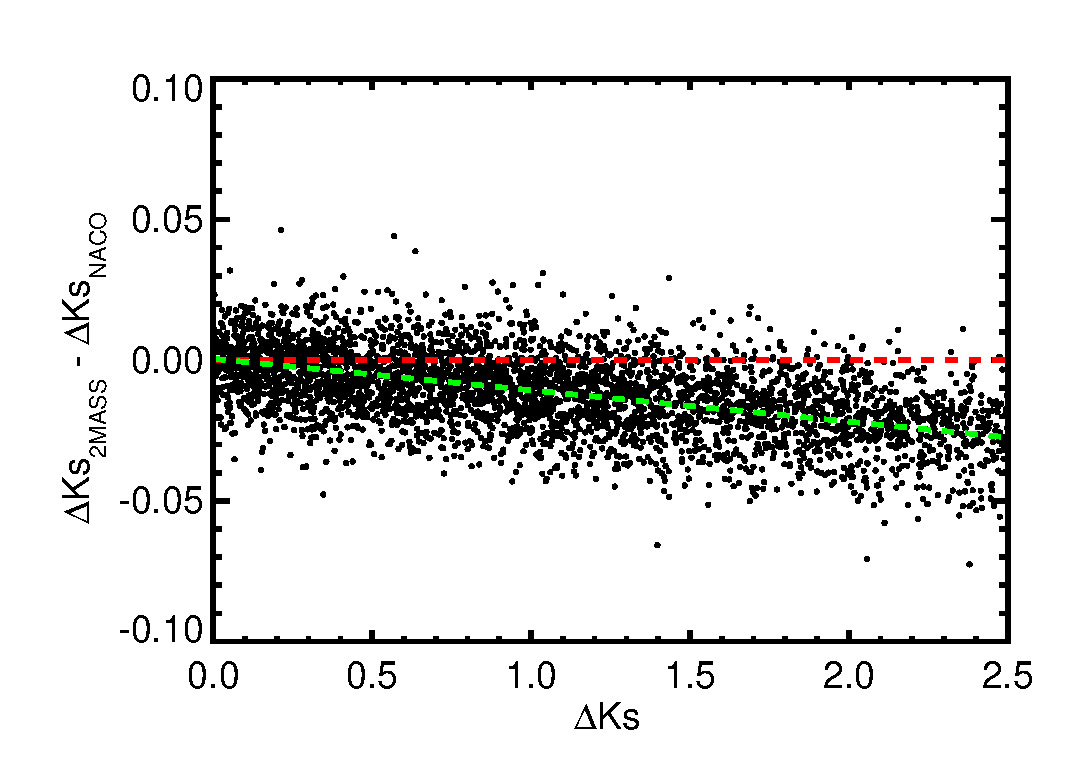
\includegraphics[width=0.47\textwidth]{NACO_Ks.eps}
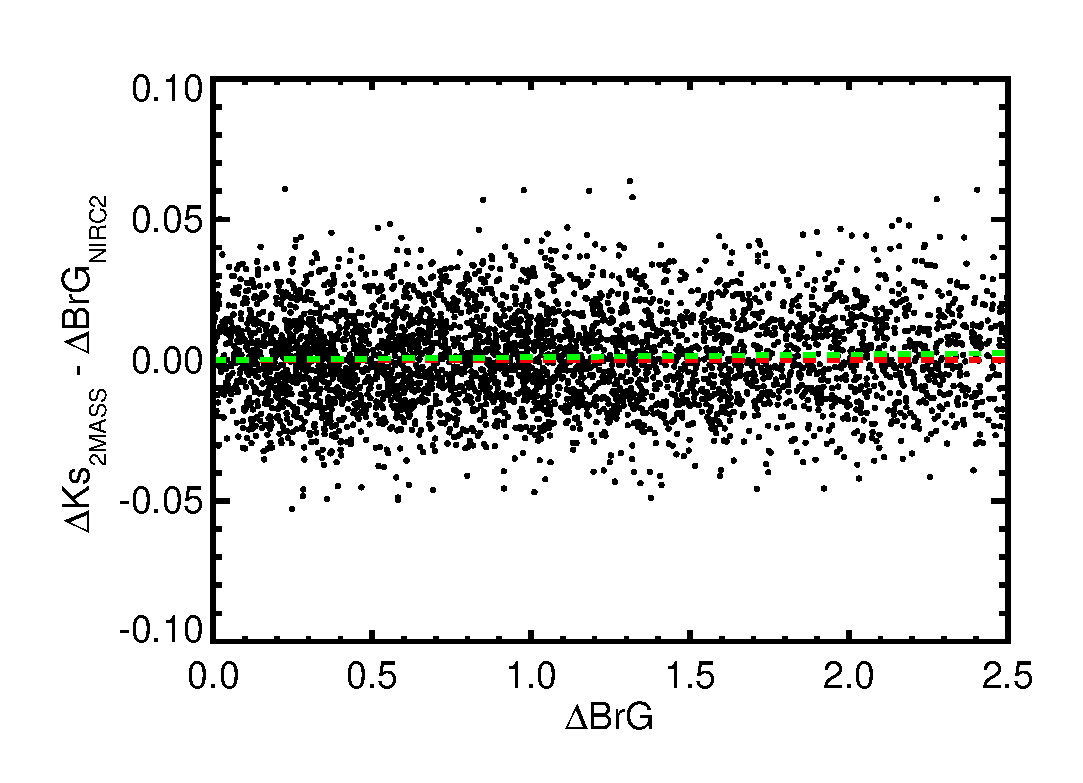
\includegraphics[width=0.47\textwidth]{NIRC2_BrG.eps}
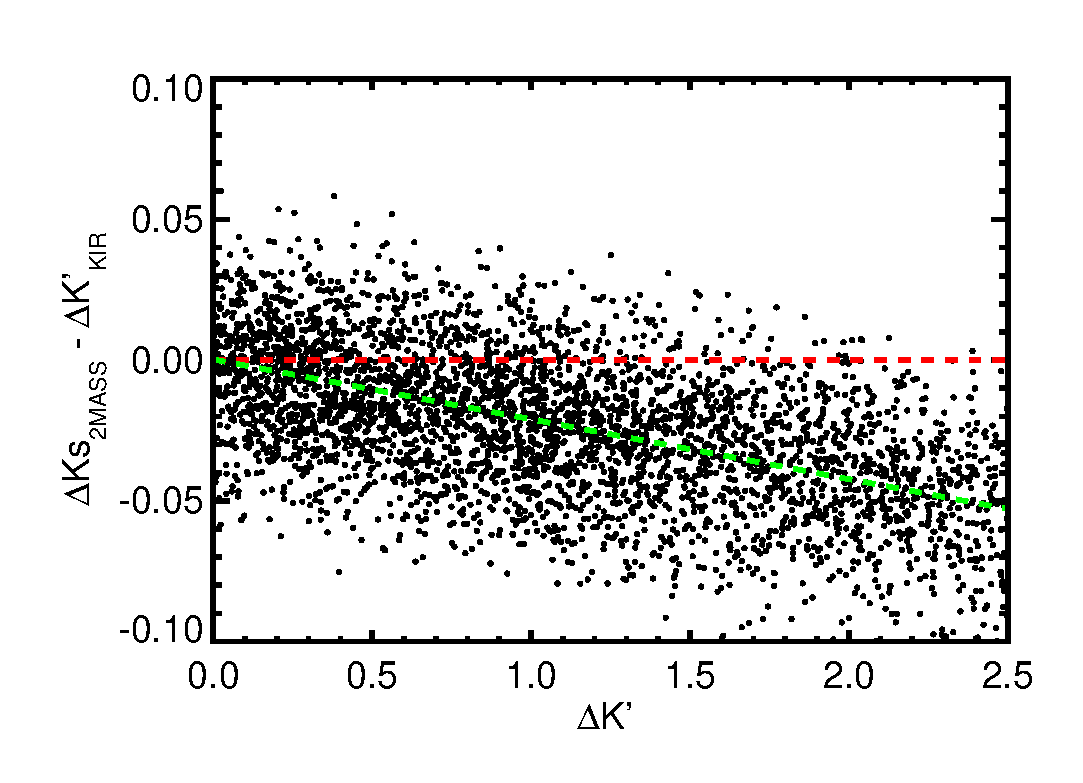
\includegraphics[width=0.47\textwidth]{KIR_Kp.eps}
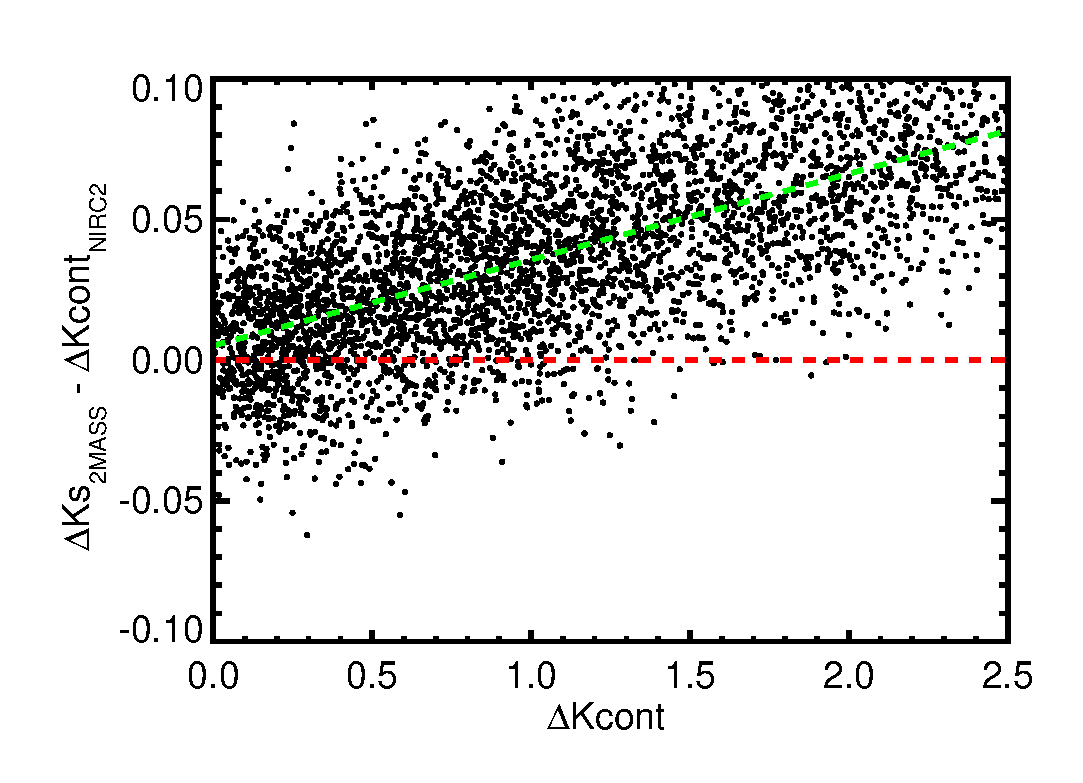
\includegraphics[width=0.47\textwidth]{NIRC2_Kcont.eps}
\caption{Difference between 2MASS $\Delta K_S$ and four example $\Delta m$ values measured from our AO imaging, built from a grid of absolutely-calibrated spectra and the filter profiles provided for each filter. No corrections are applied for the NIRC2 Bracket-Gamma (BrG) and $K_S$ (K-short) filter, as the trend is not significant compared to potential systematic issues in the calibration of the underlying spectra. }
\label{fig:mags}
\end{center}
\end{figure*}

We did not see a significant difference in any derived correction based on the metallicity of the component stars, as expected based on how [Fe/H] changes $K$-band flux levels (Figure~\ref{fig:metal}). Thus we did not attempt to include [Fe/H] in these relations. We also found no significant effect as a function of the mass of the primary. However, this was difficult to test due to limitations of the input sample. The \citet{Mann2015b} spectral sample covers K7 to M7, but is poorly populated on the extreme ends. While we can make a wide range of combinations of low-contrast systems (M0+M0 to M6+M6), we have limited options for high-contrast (where primary can only be $\sim$ K7-M1) systems where temperature effects would be most clear.

\clearpage

\section{Orbits of binaries}\label{sec:orbitplots}

Here we show diagnostic plots of each of the binaries in our sample. Details of the input points data can be found in Section~\ref{sec:ao} for data analyzed in this paper and in Section~\ref{sec:litas} for astrometry from the literature. The orbital fitting method is described in Section~\ref{sec:orbit}.

\begin{figure*}[htp]
\begin{center}
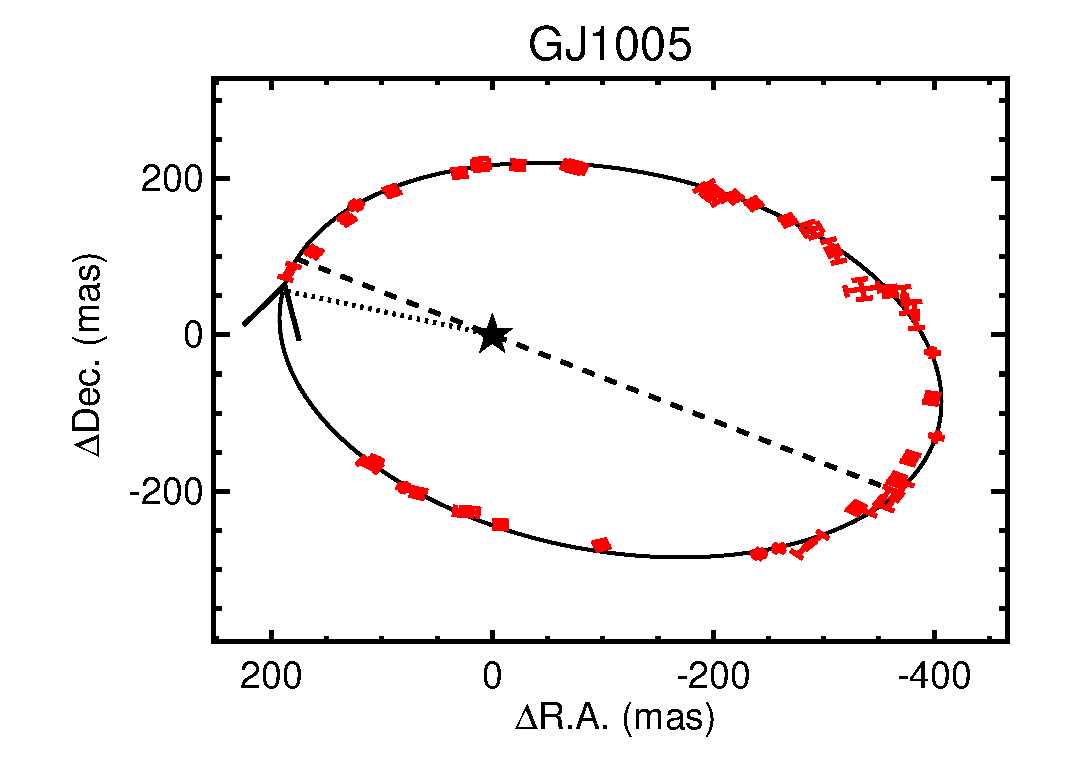
\includegraphics[width=0.32\textwidth]{Orbits/GJ1005AB.eps}
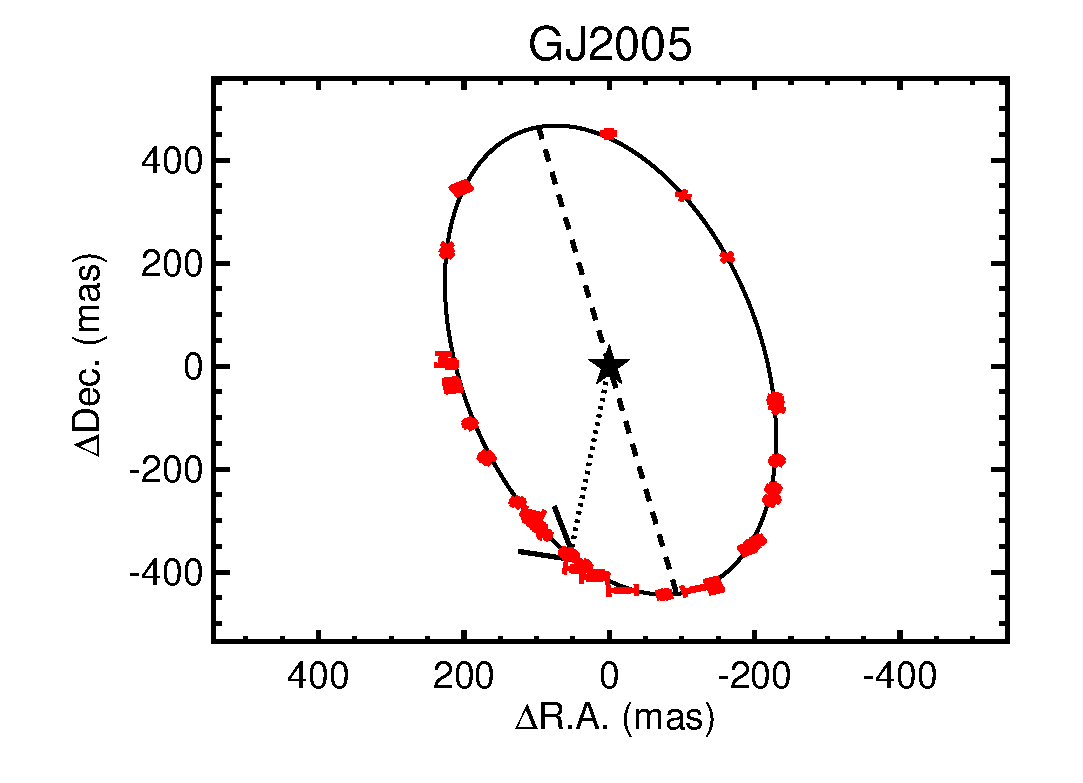
\includegraphics[width=0.32\textwidth]{Orbits/GJ2005AB.eps}
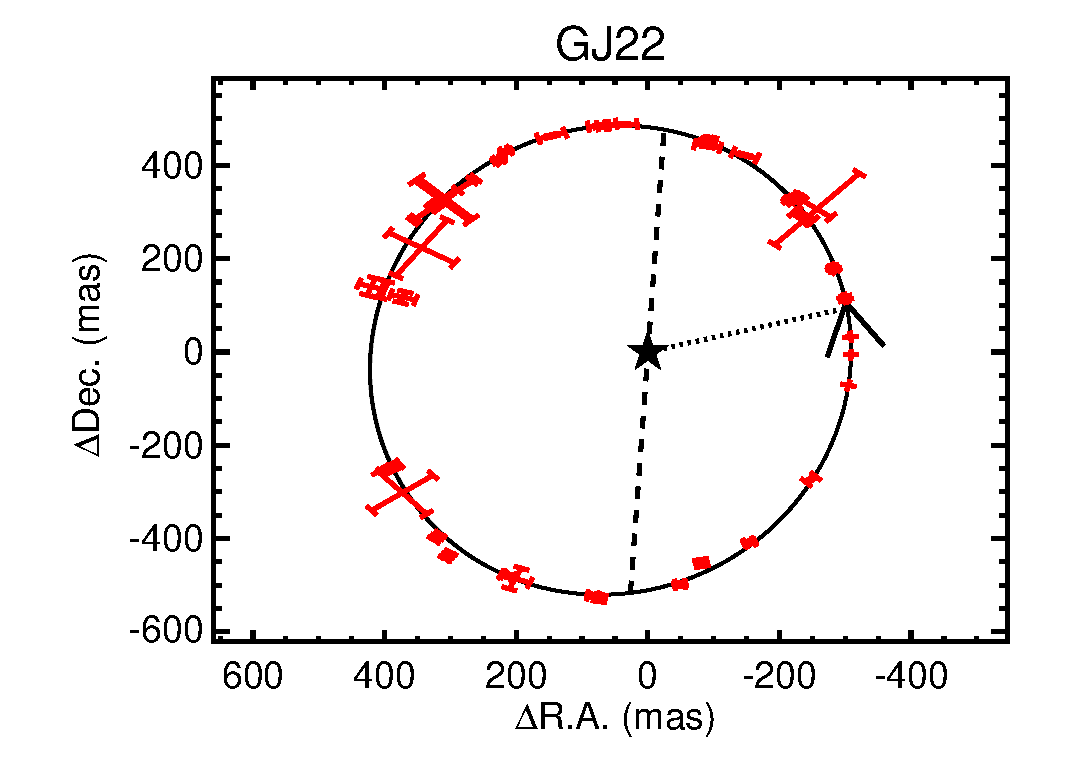
\includegraphics[width=0.32\textwidth]{Orbits/GJ22AB.eps}
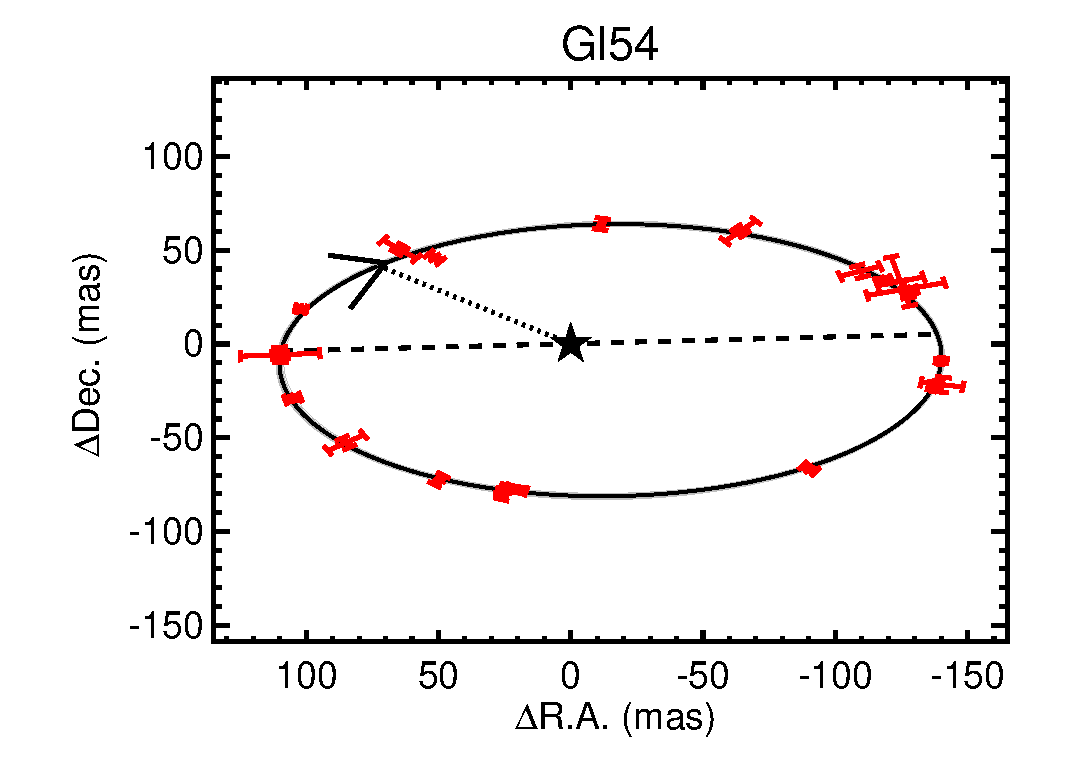
\includegraphics[width=0.32\textwidth]{Orbits/Gl54AB.eps}
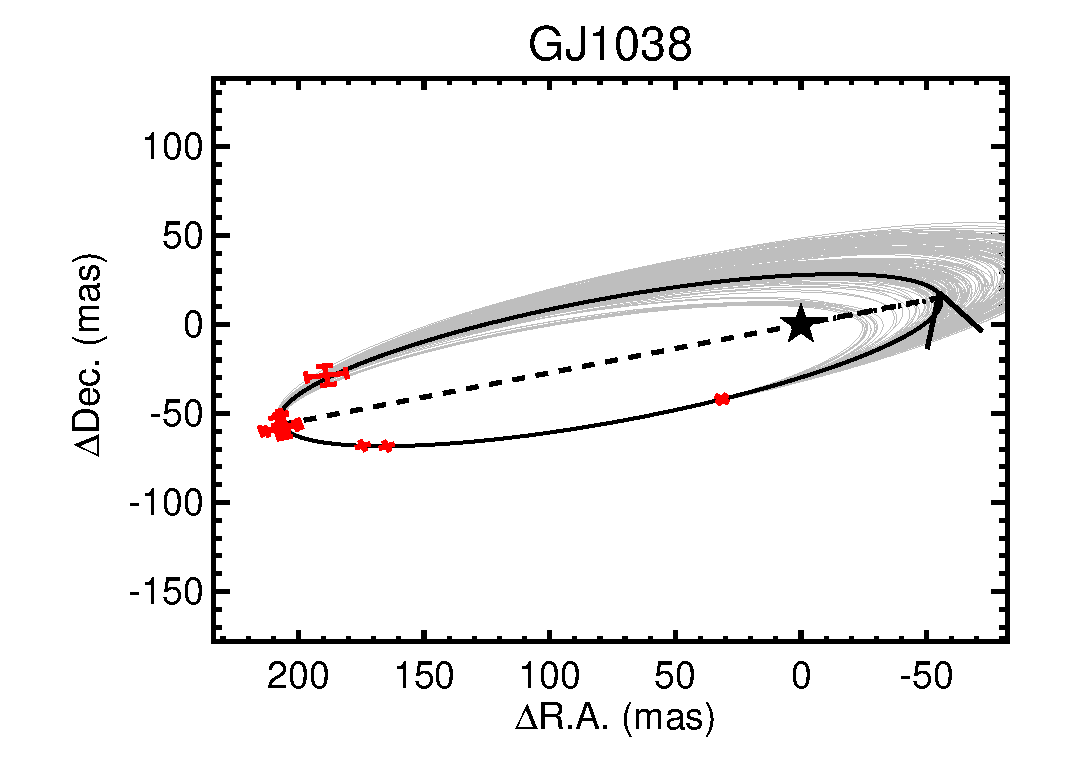
\includegraphics[width=0.32\textwidth]{Orbits/GJ1038AB.eps}
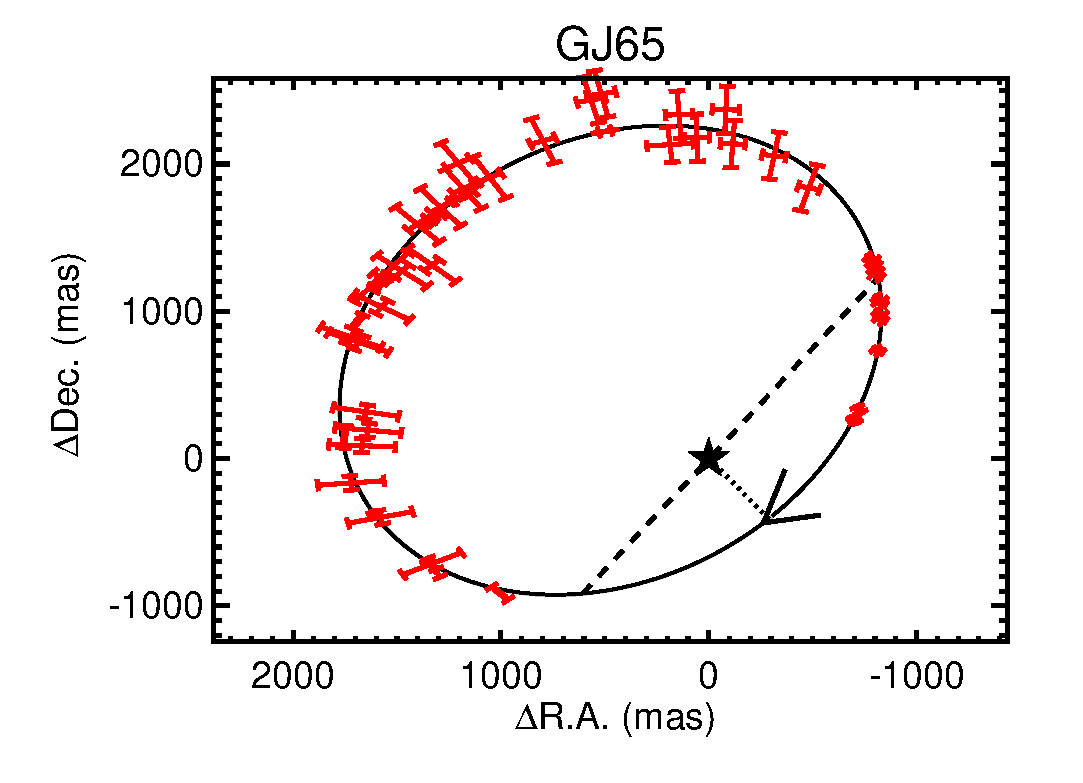
\includegraphics[width=0.32\textwidth]{Orbits/GJ65AB.eps}
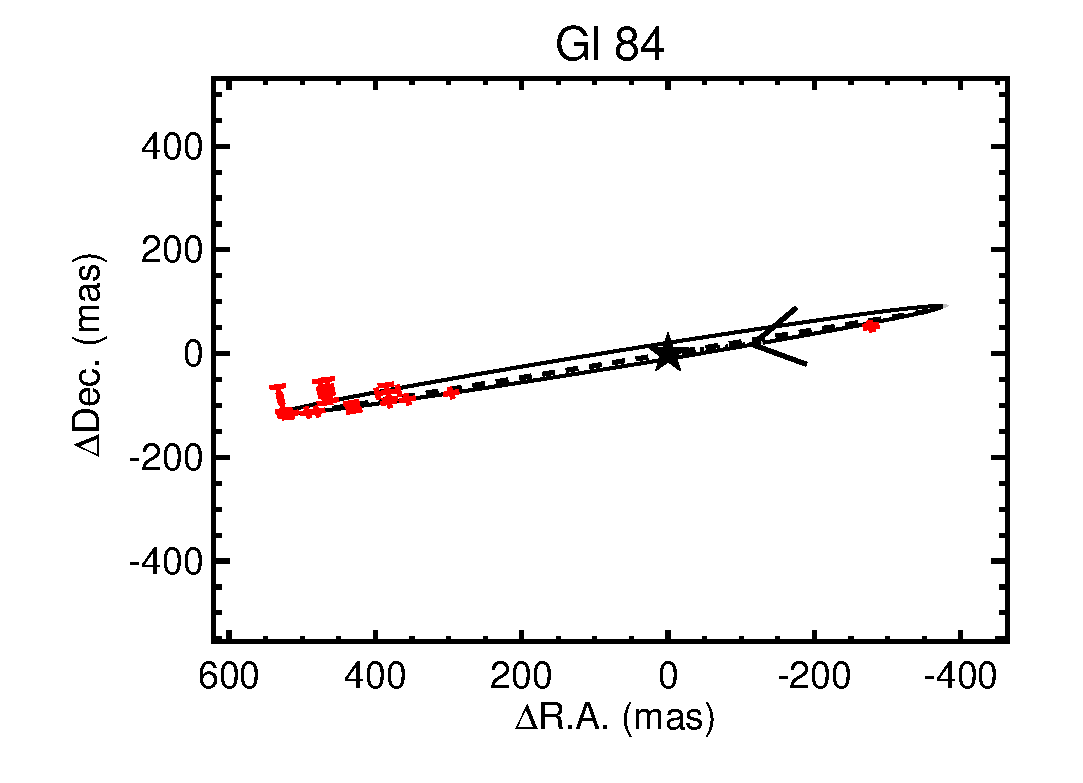
\includegraphics[width=0.32\textwidth]{Orbits/HIP9724AB.eps} %%Gl 84
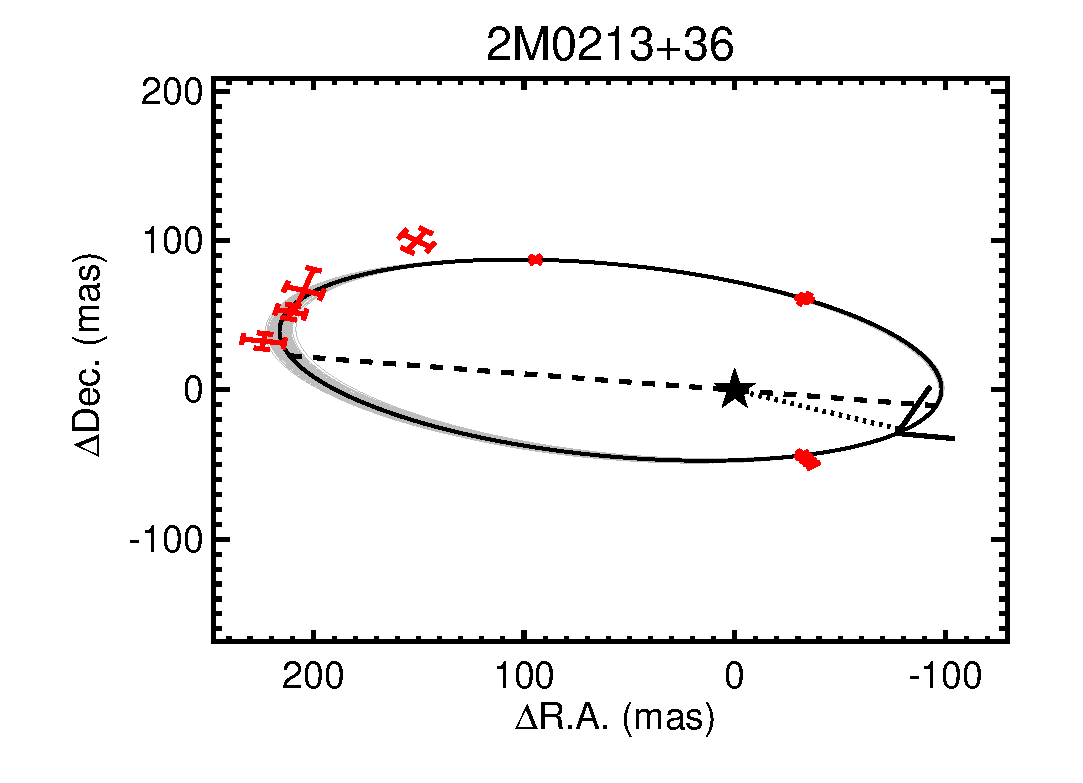
\includegraphics[width=0.32\textwidth]{Orbits/PMJ02133+3648AB.eps} 
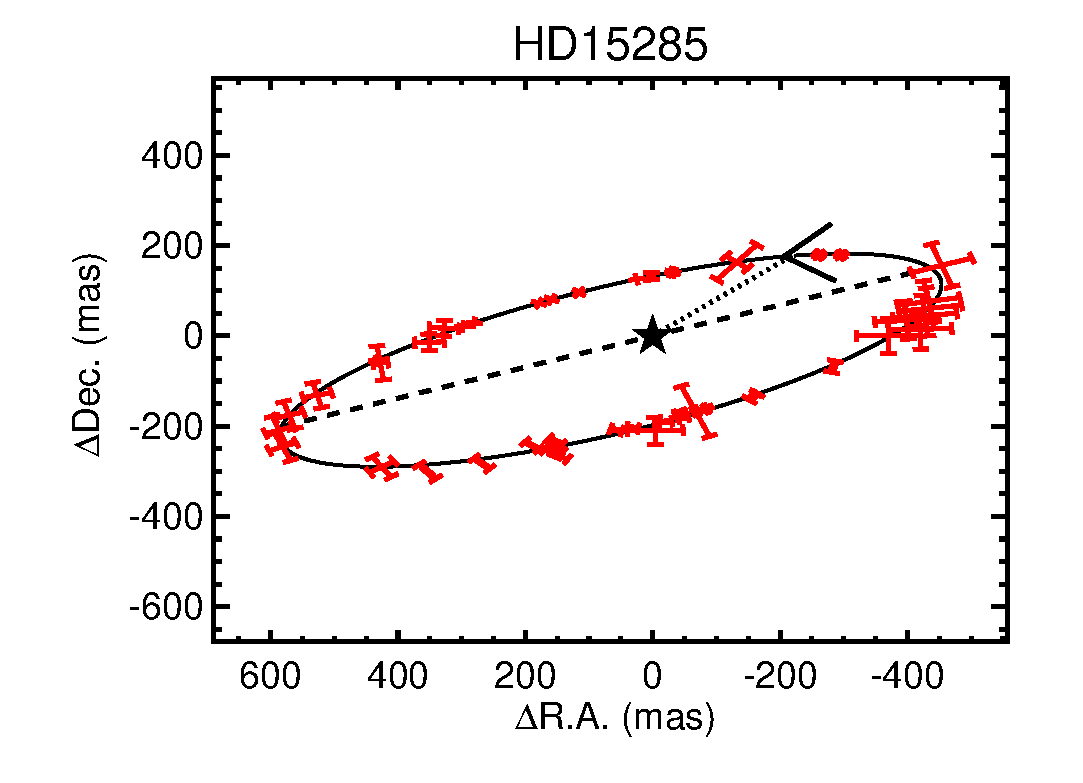
\includegraphics[width=0.32\textwidth]{Orbits/HD15285AB.eps} %% Gl98
\caption{Orbital fit for each binary fit in this paper. The black star marks the primary (always at 0, 0). The best-fit (highest likelihood) is shown as a black line, with 50 randomly selected orbit fits from the MCMC shown in grey to provide an estimate of the uncertainties. In some fits, the range of orbital solutions is so small that the grey lines are not visible underneath the best-fit black line. Points are individual separation and position angle measurements with adopted uncertainties, color-coded by the data source (Gemini/NIRI in light blue, VLT/NaCo in blue, CFHT/PUEO in light red, Keck/NIRC2 in dark red, and literature data in green). The dashed line is the line of nodes, the dotted line indicates periastron passage, and the arrow marks the direction of motion. }
\label{fig:orbits1}
\end{center}
\end{figure*}

\begin{figure*}[htp]
\begin{center}
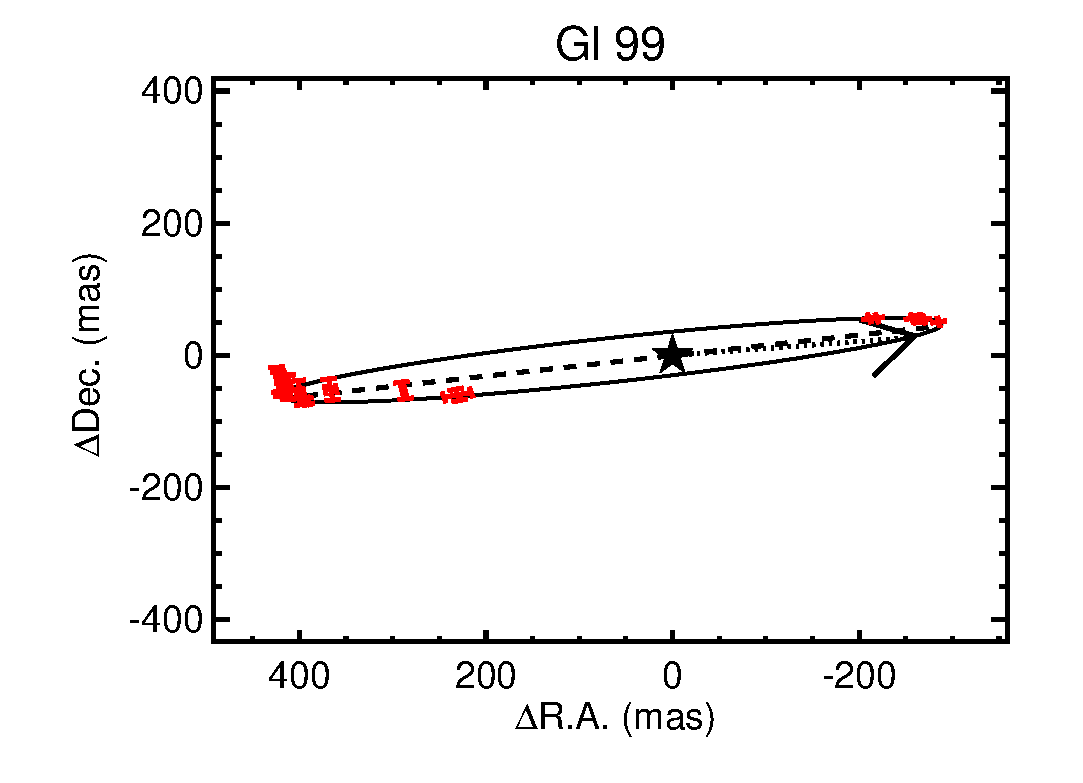
\includegraphics[width=0.32\textwidth]{Orbits/HIP11542AB.eps} %% Gl99
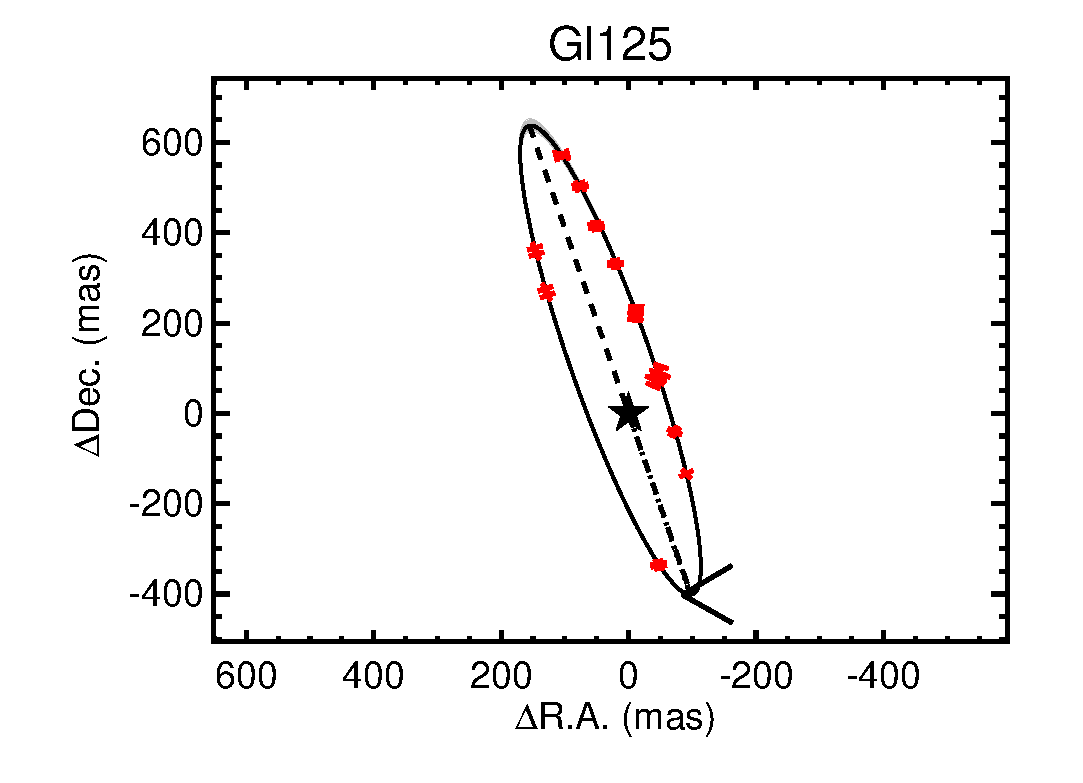
\includegraphics[width=0.32\textwidth]{Orbits/Gl125AB.eps}
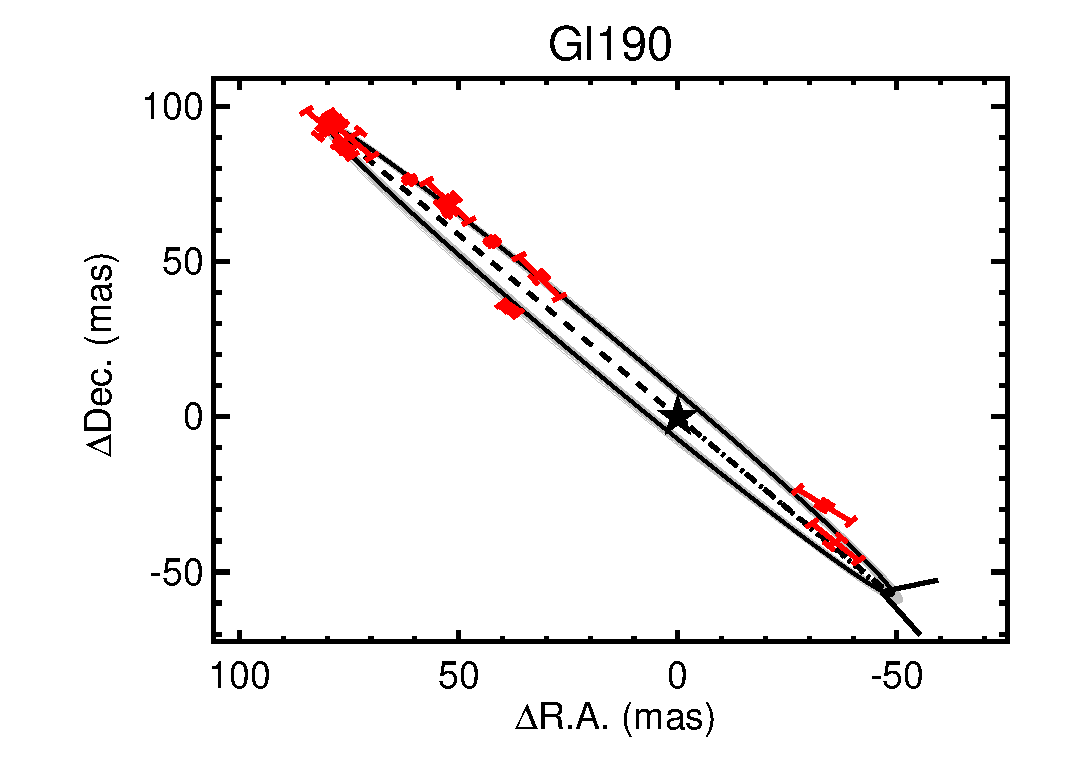
\includegraphics[width=0.32\textwidth]{Orbits/Gl190AB.eps}
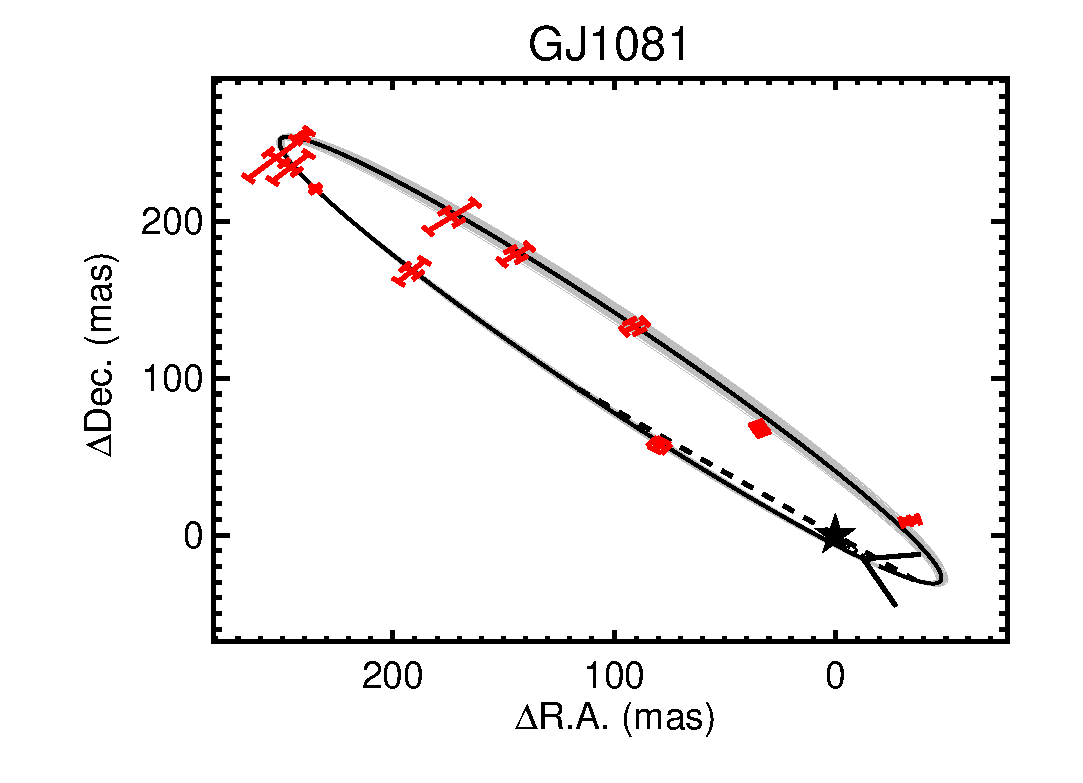
\includegraphics[width=0.32\textwidth]{Orbits/GJ1081AB.eps}
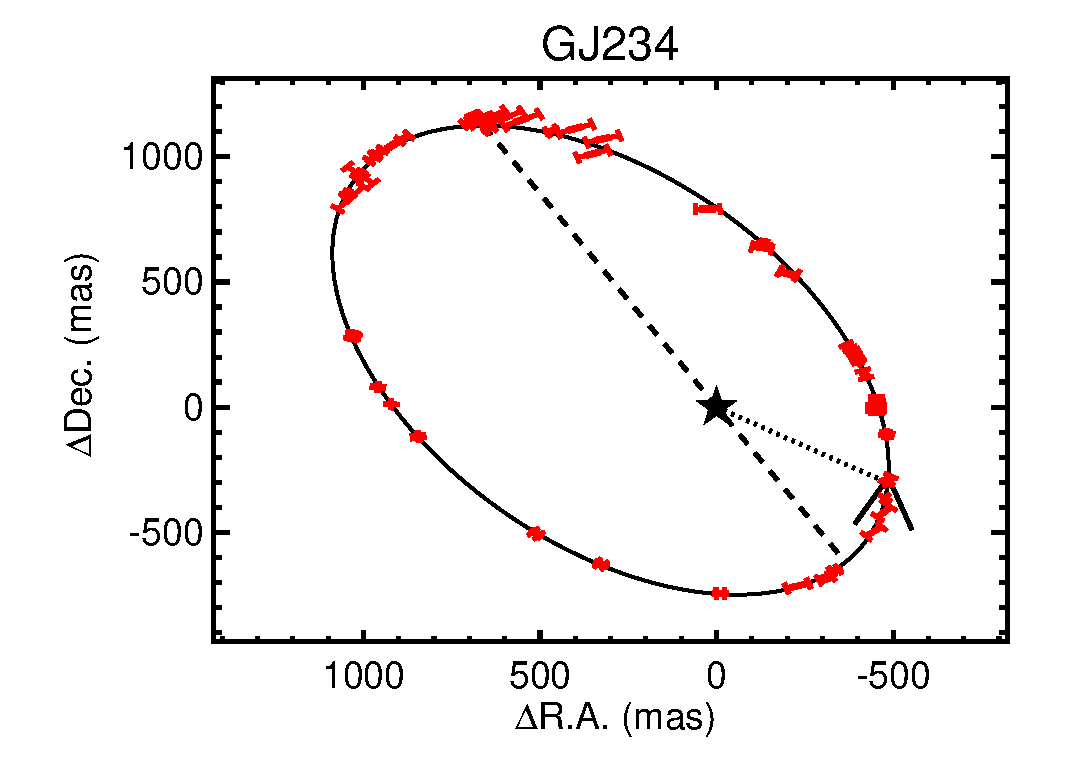
\includegraphics[width=0.32\textwidth]{Orbits/GJ234AB.eps}
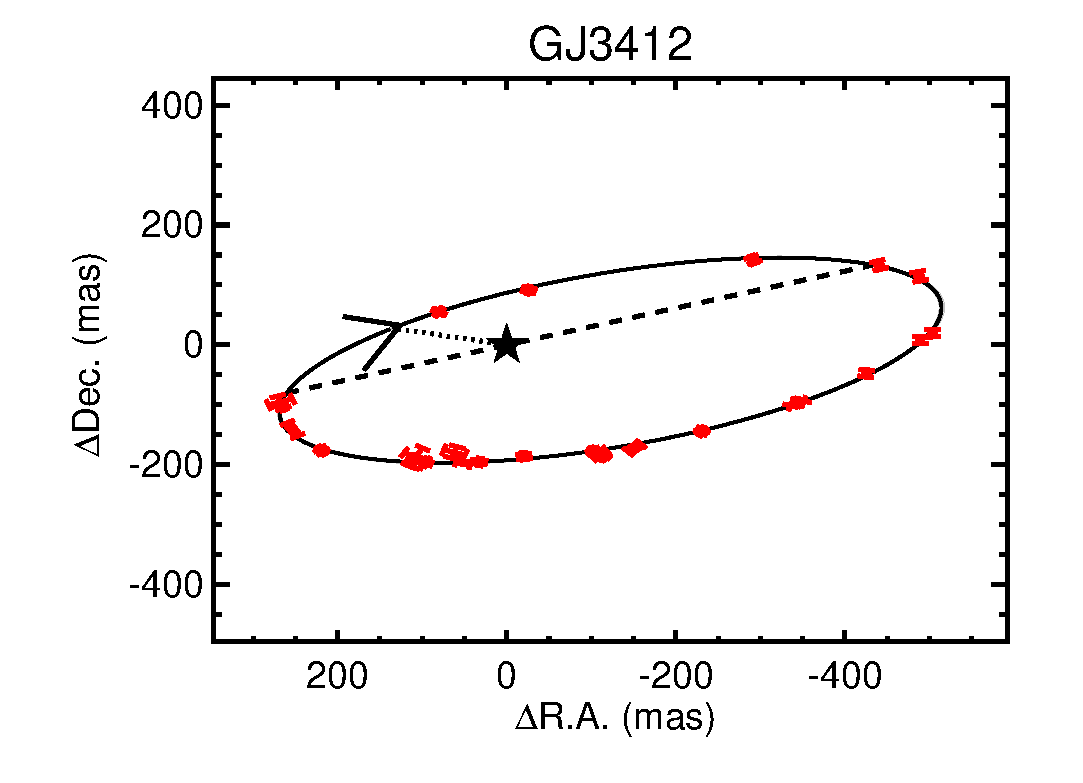
\includegraphics[width=0.32\textwidth]{Orbits/GJ3412AB.eps}
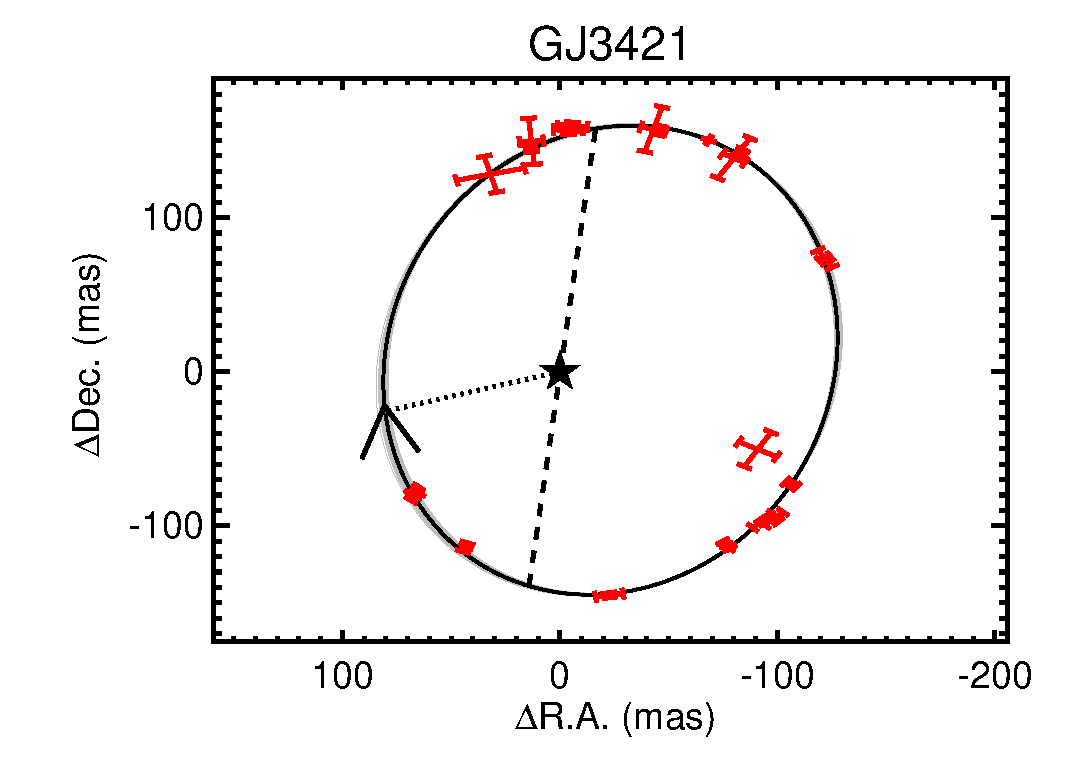
\includegraphics[width=0.32\textwidth]{Orbits/GJ3421AB.eps}
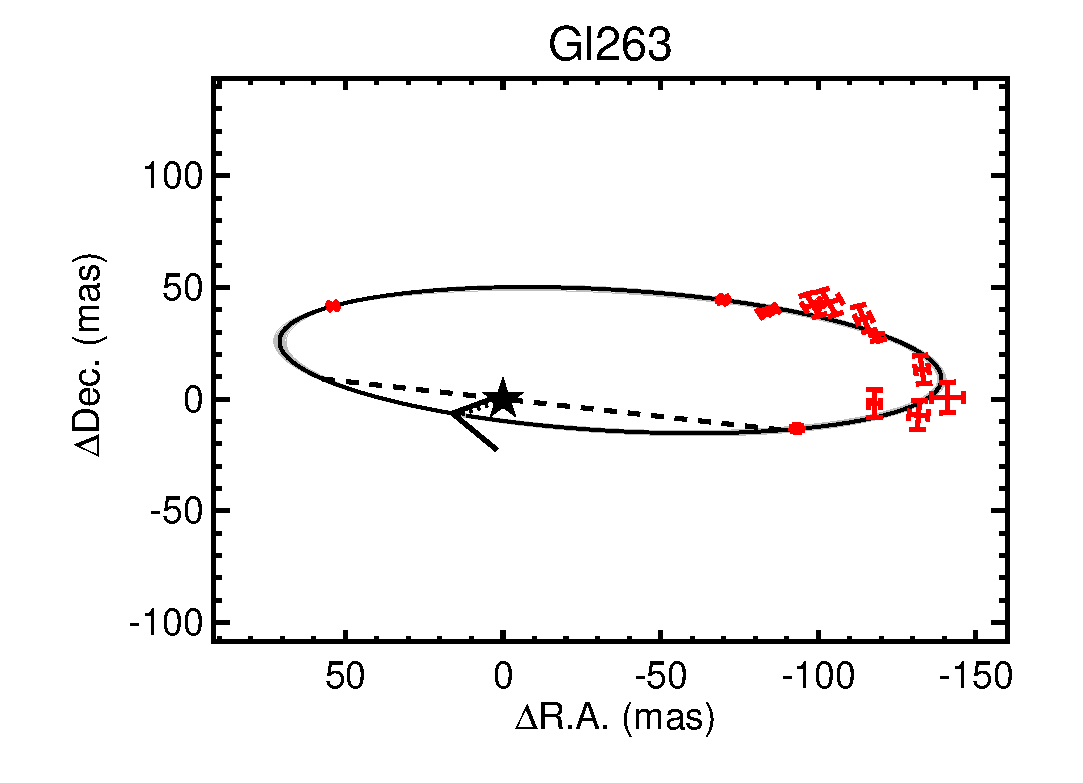
\includegraphics[width=0.32\textwidth]{Orbits/Gl263AB.eps}
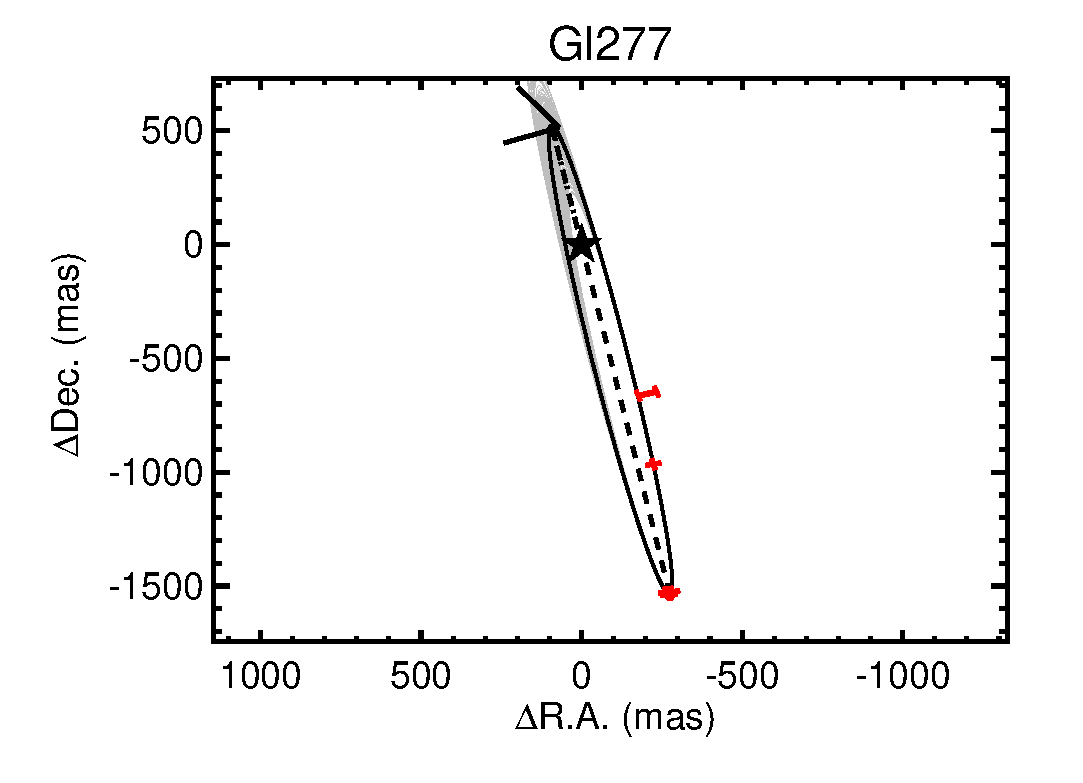
\includegraphics[width=0.32\textwidth]{Orbits/Gl277AB.eps}
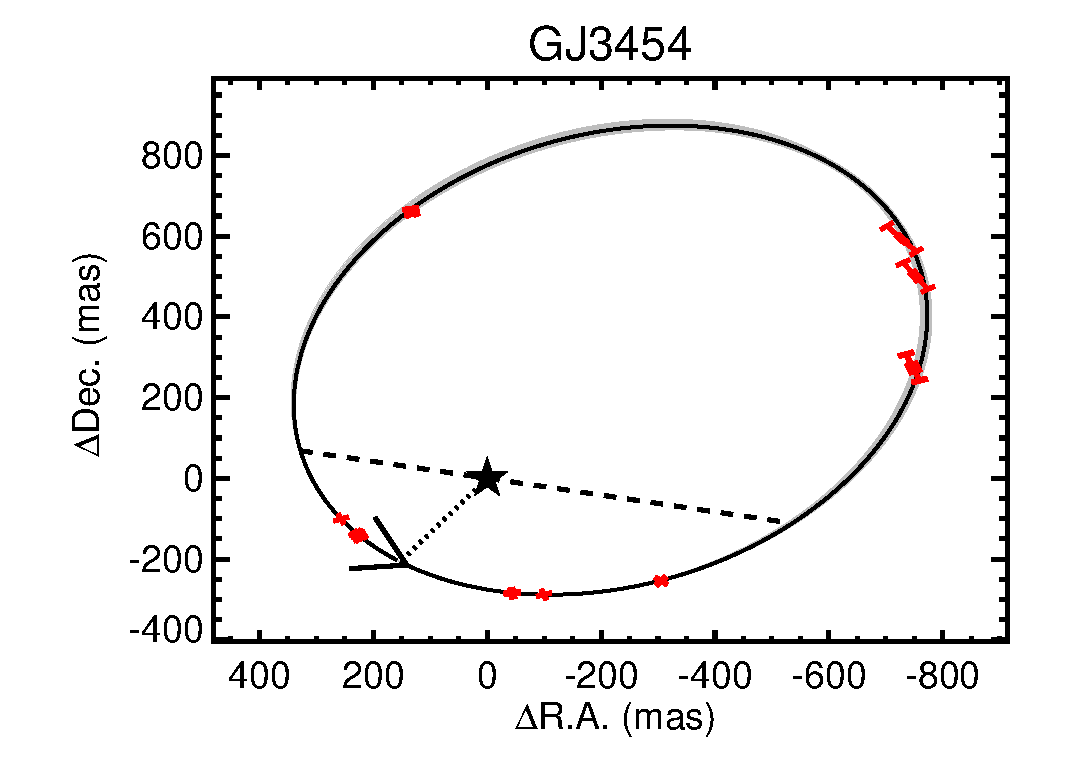
\includegraphics[width=0.32\textwidth]{Orbits/GJ3454AB.eps}
\includegraphics[width=0.32\textwidth]{Orbits/Gl301BAB.eps}
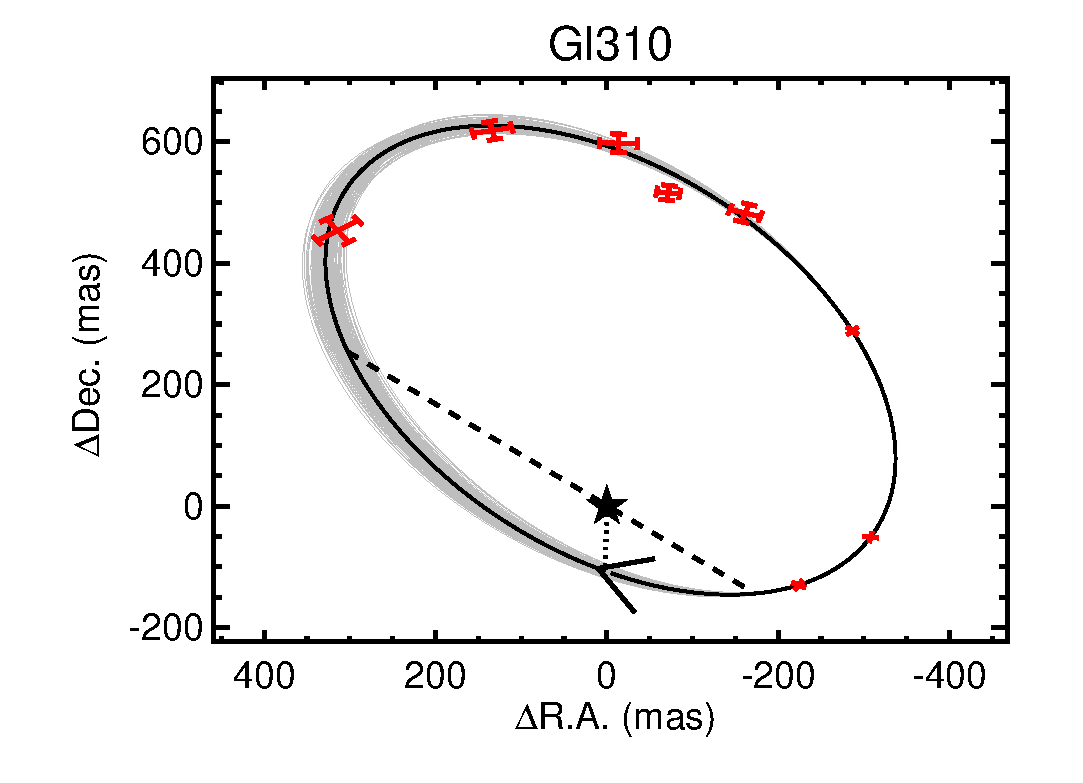
\includegraphics[width=0.32\textwidth]{Orbits/Gl310AB.eps}
\caption{Figure~\ref{fig:orbits1} continued.}
\label{fig:orbits2}
\end{center}
\end{figure*}


\begin{figure*}[htp]
\begin{center}
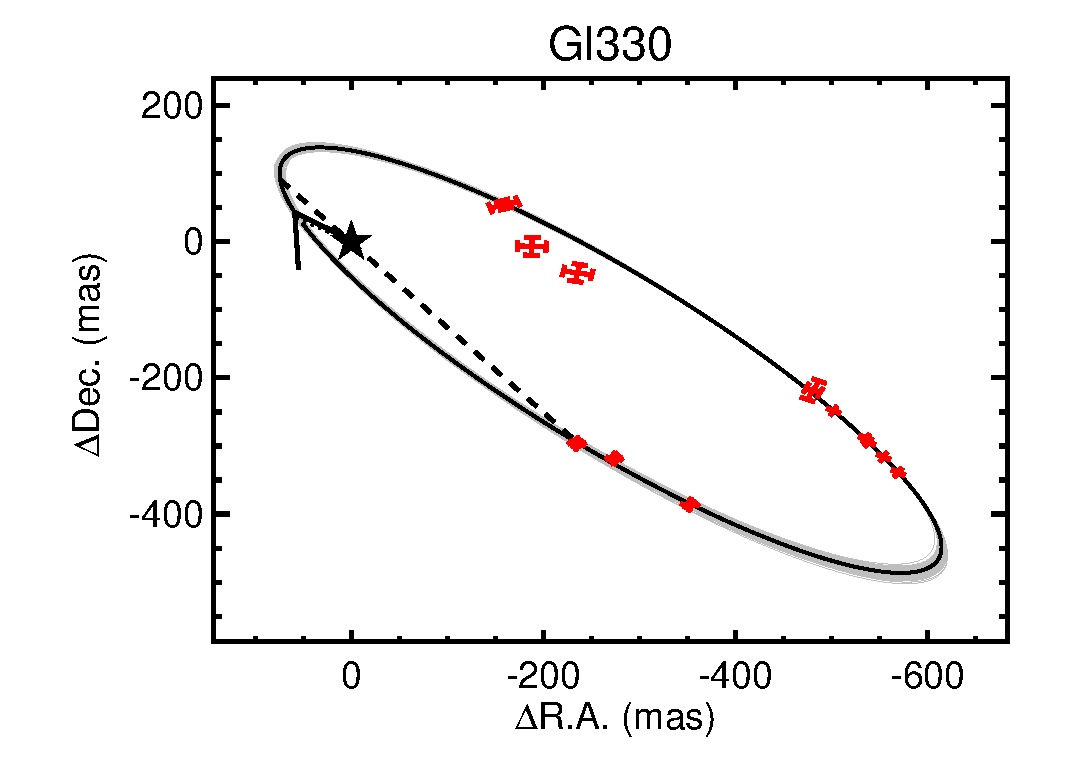
\includegraphics[width=0.32\textwidth]{Orbits/Gl330AB.eps}
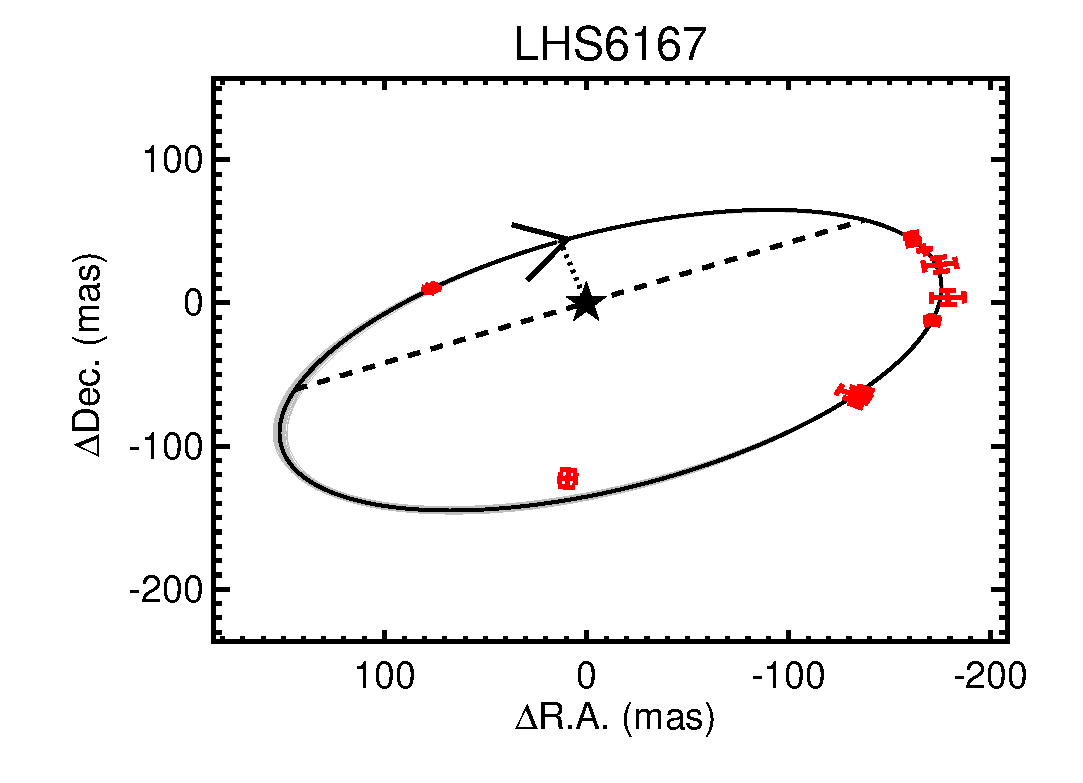
\includegraphics[width=0.32\textwidth]{Orbits/LHS6167AB.eps}
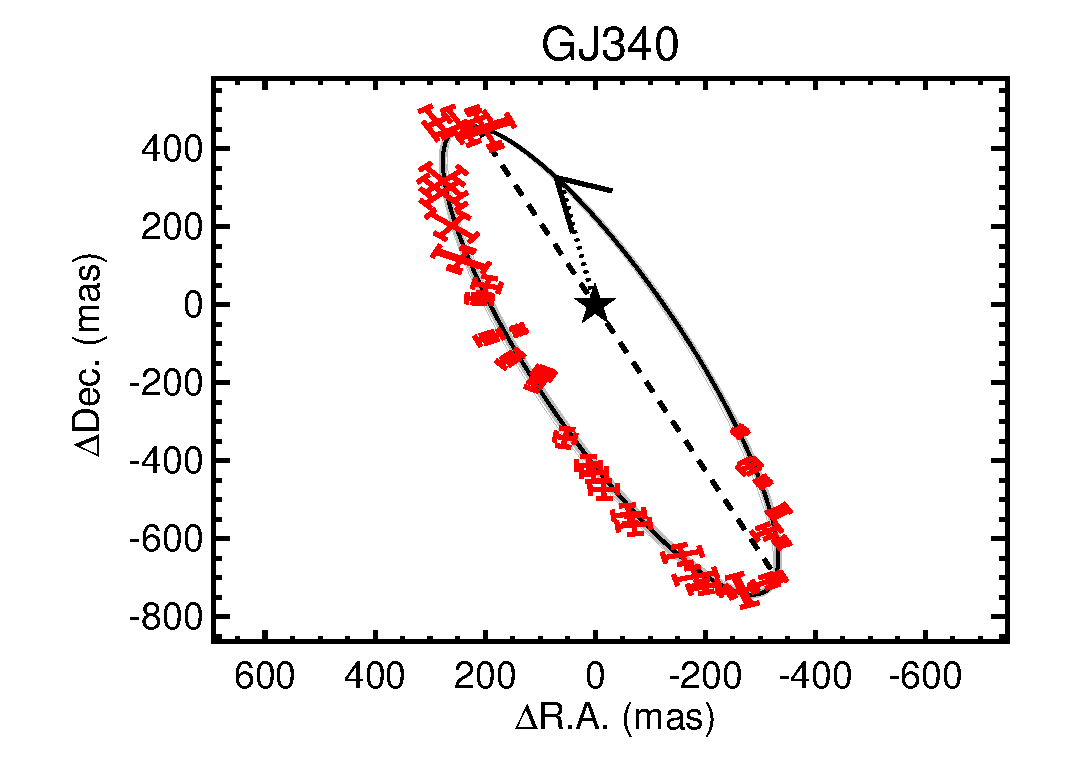
\includegraphics[width=0.32\textwidth]{Orbits/GJ340AB.eps}
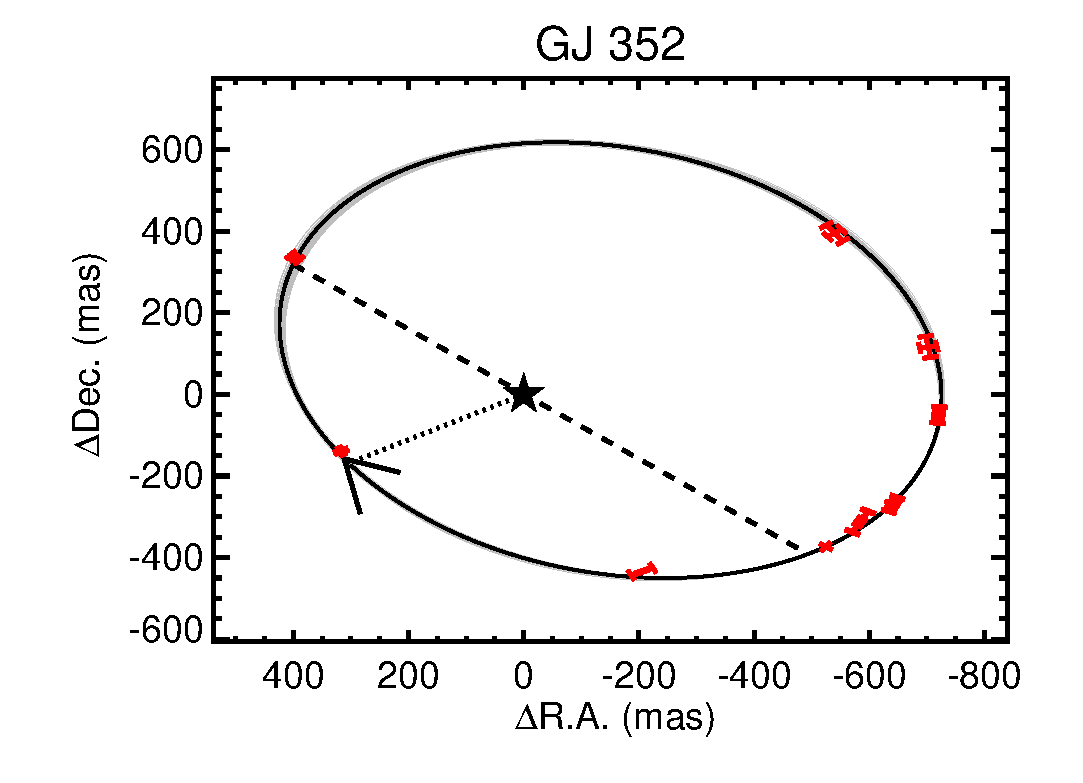
\includegraphics[width=0.32\textwidth]{Orbits/HIP46706AB.eps}%% Gl352
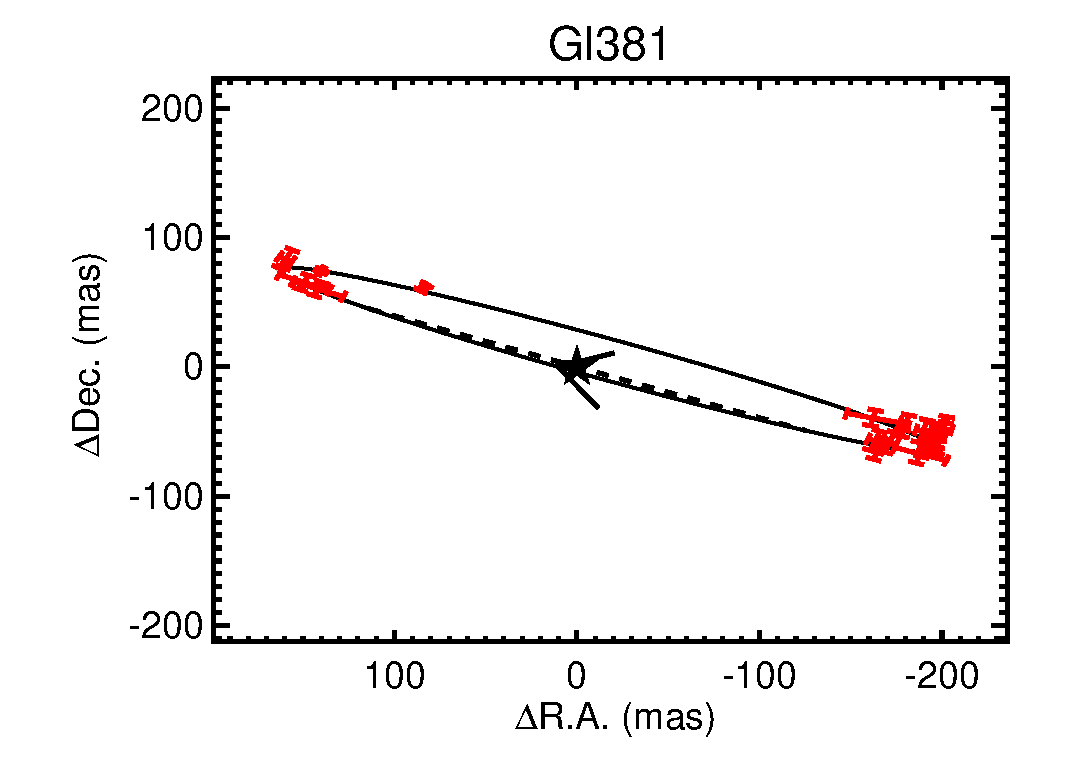
\includegraphics[width=0.32\textwidth]{Orbits/Gl381AB.eps}
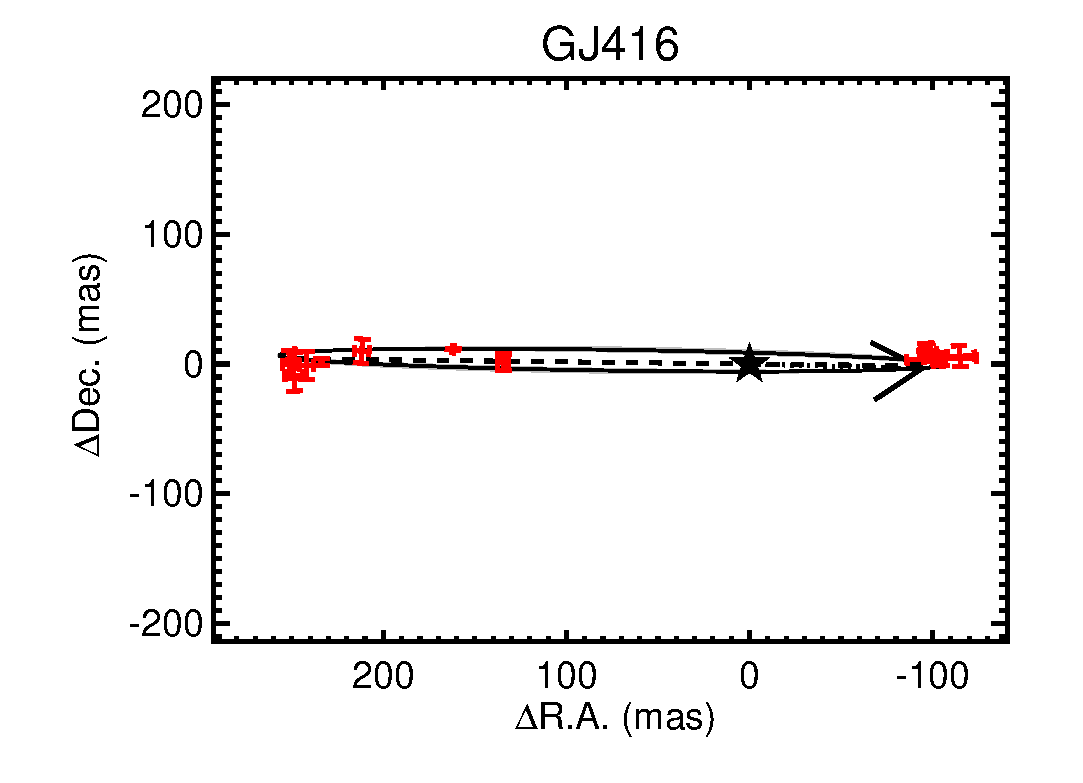
\includegraphics[width=0.32\textwidth]{Orbits/GJ416AB.eps}
\includegraphics[width=0.32\textwidth]{Orbits/Gl469AB.eps}
\includegraphics[width=0.32\textwidth]{Orbits/Gl473AB.eps}
\includegraphics[width=0.32\textwidth]{Orbits/Gl494AB.eps}
\includegraphics[width=0.32\textwidth]{Orbits/GJ570AB.eps}
\includegraphics[width=0.32\textwidth]{Orbits/GJ600AB.eps}
\includegraphics[width=0.32\textwidth]{Orbits/GJ623AB.eps}
\caption{Figure~\ref{fig:orbits1} continued.}
\label{fig:orbits3}
\end{center}
\end{figure*}

\begin{figure*}[htp]
\begin{center}
\includegraphics[width=0.32\textwidth]{Orbits/GJ1210AB.eps}
\includegraphics[width=0.32\textwidth]{Orbits/Gl660AB.eps}
\includegraphics[width=0.32\textwidth]{Orbits/GJ661AB.eps}
\includegraphics[width=0.32\textwidth]{Orbits/GJ4024AB.eps}
\includegraphics[width=0.32\textwidth]{Orbits/Gl695AB.eps}
\includegraphics[width=0.32\textwidth]{Orbits/Gl747AB.eps}
\includegraphics[width=0.32\textwidth]{Orbits/GJ748AB.eps}
\includegraphics[width=0.32\textwidth]{Orbits/HIP95995AB.eps}
\includegraphics[width=0.32\textwidth]{Orbits/HIP96656AB.eps}
\includegraphics[width=0.32\textwidth]{Orbits/GJ1245AB.eps}
\includegraphics[width=0.32\textwidth]{Orbits/Gl7912AB.eps}
\includegraphics[width=0.32\textwidth]{Orbits/Gl804AB.eps}
\caption{Figure~\ref{fig:orbits1} continued.}
\label{fig:orbits4}
\end{center}
\end{figure*}


\begin{figure*}[htp]
\begin{center}
\includegraphics[width=0.32\textwidth]{Orbits/Gl831AB.eps}
\includegraphics[width=0.32\textwidth]{Orbits/Gl844AB.eps}
\includegraphics[width=0.32\textwidth]{Orbits/HD239960AB.eps} 
\includegraphics[width=0.32\textwidth]{Orbits/GJ4287AB.eps}
\includegraphics[width=0.32\textwidth]{Orbits/Gl8934AB.eps}
\includegraphics[width=0.32\textwidth]{Orbits/Gl900AB.eps}
\includegraphics[width=0.32\textwidth]{Orbits/Gl913AB.eps}
\caption{Figure~\ref{fig:orbits1} continued.}
\label{fig:orbits5}
\end{center}
\end{figure*}

\clearpage
\startlongtable
\begin{deluxetable*}{c l l l l l l l r r}
\tablecaption{Input Astrometry and Photometry \label{tab:astrom} }
\tablehead{
   \colhead{UT Date\tablenotemark{a}} & \colhead{$\rho$} & \colhead{$\theta$} & \colhead{Filter}  & \colhead{$\Delta$m} & \colhead{Source}  \\
    \colhead{(YYYY-MM-DD)} & \colhead{(mas)} & \colhead{(degrees)} & \colhead{} & \colhead{(mag)} & \colhead{}
}
\startdata
\multicolumn{6}{c}{GJ 1005}  \\
\hline
1993-08-09 & $397.0\pm5.0$ & $236.10\pm0.90$ & \nodata & \nodata & \citet{Benedict2016}\\
1994-05-22 & $286.0\pm5.0$ & $200.20\pm0.90$ & \nodata & \nodata & \citet{Benedict2016}\\
1994-08-15 & $242.0\pm5.0$ & $181.70\pm0.90$ & \nodata & \nodata & \citet{Benedict2016}\\
1994-10-15 & $213.0\pm5.0$ & $161.70\pm0.90$ & \nodata & \nodata & \citet{Benedict2016}\\
1994-12-01 & $194.0\pm5.0$ & $146.60\pm0.90$ & \nodata & \nodata & \citet{Benedict2016}\\
1995-06-25 & $193.0\pm5.0$ & $56.80\pm0.90$ & \nodata & \nodata & \citet{Benedict2016}\\
1995-08-01 & $198.0\pm5.0$ & $41.70\pm0.90$ & \nodata & \nodata & \citet{Benedict2016}\\
1995-09-11 & $205.0\pm5.0$ & $26.30\pm0.90$ & \nodata & \nodata & \citet{Benedict2016}\\
1995-10-30 & $209.0\pm5.0$ & $8.20\pm0.90$ & \nodata & \nodata & \citet{Benedict2016}\\
1995-12-11 & $218.0\pm5.0$ & $353.90\pm0.90$ & \nodata & \nodata & \citet{Benedict2016}\\
1996-06-02 & $281.0\pm5.0$ & $308.80\pm0.90$ & \nodata & \nodata & \citet{Benedict2016}\\
1996-06-24 & $290.0\pm5.0$ & $305.30\pm0.90$ & \nodata & \nodata & \citet{Benedict2016}\\
1996-07-28 & $305.0\pm5.0$ & $298.70\pm0.90$ & \nodata & \nodata & \citet{Benedict2016}\\
1996-12-25 & $364.0\pm5.0$ & $278.80\pm0.90$ & \nodata & \nodata & \citet{Benedict2016}\\
1997-06-29 & $406.0\pm5.0$ & $258.50\pm0.90$ & \nodata & \nodata & \citet{Benedict2016}\\
1997-11-10 & $410.0\pm5.0$ & $247.40\pm0.90$ & \nodata & \nodata & \citet{Benedict2016}\\
1997-12-18 & $410.0\pm5.0$ & $243.20\pm0.90$ & \nodata & \nodata & \citet{Benedict2016}\\
2000-08-20 & $227.0\pm6.0$ & $340.9\pm2.5$ & BrG & $1.068\pm0.013$ & CFHT/PUEO\\
2000-12-12 & $265.0\pm4.0$ & $312.4\pm2.6$ & K & $1.070\pm0.025$ & CFHT/PUEO\\
2000-12-12 & $274.4\pm2.0$ & $312.0\pm2.6$ & H & $1.110\pm0.070$ & CFHT/PUEO\\
2001-08-04 & $376.4\pm1.9$ & $276.8\pm2.5$ & BrG & $1.140\pm0.040$ & CFHT/PUEO\\
2001-08-31 & $383.7\pm2.0$ & $273.8\pm2.5$ & FeII & $1.190\pm0.017$ & CFHT/PUEO\\
2002-06-25 & $420.0\pm3.0$ & $240.7\pm2.5$ & FeII & $1.180\pm0.040$ & CFHT/PUEO\\
2002-09-11 & $410.2\pm1.6$ & $238.8\pm2.5$ & PaBe & $1.220\pm0.040$ & CFHT/PUEO\\
2002-11-21 & $392.8\pm1.6$ & $227.0\pm2.5$ & H2v=2-1 & $1.110\pm0.050$ & CFHT/PUEO\\
2003-10-16 & $227.0\pm5.0$ & $174.1\pm2.7$ & H2v=2-1 & $1.200\pm0.090$ & CFHT/PUEO\\
2003-12-10 & $210.8\pm2.1$ & $157.80\pm0.40$ & FeII & $1.260\pm0.040$ & VLT/NaCo\\
2004-01-08 & $199.4\pm2.9$ & $146.2\pm2.7$ & BrG & $1.110\pm0.060$ & CFHT/PUEO\\
2004-07-02 & $200.5\pm2.1$ & $66.3\pm2.6$ & H2v=2-1 & $1.310\pm0.040$ & CFHT/PUEO\\
2004-09-24 & $206.6\pm2.1$ & $36.70\pm0.50$ & FeII & $1.239\pm0.011$ & VLT/NaCo\\
2004-12-28 & $218.0\pm7.0$ & $2.7\pm1.9$ & \nodata & \nodata & \citet{Doc2006i}\\
2005-10-16 & $327.0\pm5.0$ & $289.1\pm2.5$ & H2v=2-1 & $1.110\pm0.040$ & CFHT/PUEO\\
2007-08-29 & $369.5\pm2.0$ & $220.80\pm0.40$ & FeII & $1.211\pm0.023$ & VLT/NaCo\\
2010-08-05 & $340\pm15$ & $279.9\pm2.1$ & \nodata & \nodata & \citet{RDR2015}\\
2014-07-30 & $340\pm15$ & $314.050\pm0.100$ & K$_{\rm cont}$ & $1.196\pm0.012$ & Keck/NIRC2\\
2014-11-08 & $319.0\pm8.0$ & $294.9\pm1.6$ & \nodata & \nodata & \citet{Tok2017b}\\
2015-06-23 & $319.0\pm8.0$ & $266.750\pm0.100$ & K$_{\rm cont}$ & $1.203\pm0.011$ & Keck/NIRC2\\
2015-11-27 & $319.0\pm8.0$ & $252.060\pm0.100$ & K$_{\rm cont}$ & $1.209\pm0.011$ & Keck/NIRC2\\
2016-09-20 & $376.5\pm1.2$ & $223.600\pm0.100$ & K$_{\rm cont}$ & $1.211\pm0.017$ & Keck/NIRC2\\
\hline
\multicolumn{6}{c}{GJ 2005}  \\
\hline
2000-08-16 & $229.0\pm3.0$ & $86.8\pm2.8$ & K' & $0.342\pm0.029$ & CFHT/PUEO\\
2000-11-01 & $218.0\pm5.0$ & $88.90\pm0.80$ & \nodata & \nodata & \citet{Koh2012}\\
2000-12-12 & $220.0\pm6.0$ & $99.5\pm2.8$ & K & $0.360\pm0.040$ & CFHT/PUEO\\
2001-01-09 & $220.0\pm6.0$ & $100.4\pm2.4$ & \nodata & \nodata & \citet{Koh2012}\\
2001-07-02 & $222.0\pm4.0$ & $120.30\pm0.50$ & \nodata & \nodata & \citet{Koh2012}\\
2001-12-07 & $244.0\pm4.0$ & $136.10\pm0.50$ & \nodata & \nodata & \citet{Koh2012}\\
2001-12-11 & $246.0\pm6.0$ & $136.10\pm0.50$ & \nodata & \nodata & \citet{Koh2012}\\
2002-07-24 & $293.0\pm3.0$ & $154.50\pm0.80$ & \nodata & \nodata & \citet{Sef2008}\\
2002-09-11 & $305.0\pm2.1$ & $159.8\pm2.5$ & H & $0.340\pm0.021$ & CFHT/PUEO\\
2002-10-22 & $315.0\pm3.0$ & $159.70\pm0.80$ & \nodata & \nodata & \citet{Sef2008}\\
2002-11-15 & $320.0\pm3.0$ & $161.10\pm0.80$ & \nodata & \nodata & \citet{Sef2008}\\
2002-12-16 & $327.0\pm4.0$ & $162.80\pm0.60$ & \nodata & \nodata & \citet{Koh2012}\\
2003-01-26 & $339.0\pm3.0$ & $164.80\pm0.80$ & \nodata & \nodata & \citet{Sef2008}\\
2003-05-25 & $367.0\pm3.0$ & $170.80\pm0.70$ & \nodata & \nodata & \citet{Sef2008}\\
2003-06-12 & $370.0\pm3.0$ & $171.40\pm0.70$ & \nodata & \nodata & \citet{Sef2008}\\
2003-06-17 & $371.0\pm3.0$ & $171.60\pm0.70$ & \nodata & \nodata & \citet{Sef2008}\\
2003-06-28 & $373.0\pm3.0$ & $171.90\pm0.70$ & \nodata & \nodata & \citet{Sef2008}\\
2003-09-05 & $387.0\pm3.0$ & $174.50\pm0.70$ & \nodata & \nodata & \citet{Sef2008}\\
2003-09-15 & $389.0\pm3.0$ & $174.80\pm0.70$ & \nodata & \nodata & \citet{Sef2008}\\
2003-10-16 & $397.0\pm4.0$ & $173.7\pm2.5$ & K' & $0.280\pm0.080$ & CFHT/PUEO\\
2003-12-10 & $406.0\pm3.0$ & $177.90\pm0.70$ & \nodata & \nodata & \citet{Sef2008}\\
2003-12-13 & $406.0\pm4.0$ & $178.20\pm0.50$ & \nodata & \nodata & \citet{Koh2012}\\
2004-01-08 & $412.2\pm2.6$ & $177.2\pm2.5$ & K' & $0.170\pm0.060$ & CFHT/PUEO\\
2004-07-02 & $436.1\pm2.0$ & $182.4\pm2.5$ & K' & $0.321\pm0.015$ & CFHT/PUEO\\
2004-12-12 & $450.0\pm5.0$ & $189.70\pm0.50$ & \nodata & \nodata & \citet{Koh2012}\\
2005-09-25 & $450\pm12$ & $189.70\pm0.50$ & \nodata & \nodata & \citet{Koh2012}\\
2005-10-13 & $448.8\pm1.8$ & $195.7\pm2.5$ & K' & $0.264\pm0.026$ & CFHT/PUEO\\
2006-09-02 & $403.0\pm7.0$ & $195.7\pm2.5$ & \nodata & \nodata & \citet{Koh2012}\\
2006-10-31 & $399.0\pm4.0$ & $209.60\pm0.70$ & \nodata & \nodata & \citet{Koh2012}\\
2006-11-28 & $396.0\pm5.0$ & $211.00\pm0.60$ & \nodata & \nodata & \citet{Koh2012}\\
2007-07-17 & $343.0\pm3.0$ & $220.60\pm0.80$ & \nodata & \nodata & \citet{Sef2008}\\
2007-07-25 & $342.0\pm3.0$ & $221.00\pm0.80$ & \nodata & \nodata & \citet{Sef2008}\\
2007-09-16 & $328.0\pm4.0$ & $223.50\pm0.50$ & \nodata & \nodata & \citet{Koh2012}\\
2008-02-01 & $295.0\pm4.0$ & $231.50\pm0.50$ & \nodata & \nodata & \citet{Koh2012}\\
2008-09-18 & $245.4\pm1.2$ & $250.40\pm0.40$ & FeII & $0.338\pm0.013$ & VLT/NaCo\\
2008-10-18 & $240.0\pm4.0$ & $252.60\pm0.50$ & \nodata & \nodata & \citet{Koh2012}\\
2008-11-06 & $237.0\pm4.0$ & $254.60\pm0.50$ & \nodata & \nodata & \citet{Koh2012}\\
2010-08-02 & $266.80\pm0.40$ & $322.480\pm0.100$ & Lp & $0.290\pm0.030$ & Keck/NIRC2\\
2011-07-01 & $346.50\pm0.24$ & $342.900\pm0.040$ & K & $0.329\pm0.028$ & Keck/NIRC2\\
2012-12-05 & $451.1\pm1.7$ & $0.10\pm0.40$ & L & $0.347\pm0.011$ & VLT/NaCo\\
2015-11-30 & $401.0\pm8.0$ & $30.5\pm1.6$ & \nodata & \nodata & \citet{Tok2017b}\\
2016-09-20 & $320.730\pm0.100$ & $44.070\pm0.017$ & K' & $0.313\pm0.010$ & Keck/NIRC2\\
2016-10-14 & $313.7\pm1.2$ & $45.40\pm0.40$ & Ks & $0.324\pm0.010$ & VLT/NaCo\\
\hline
\multicolumn{6}{c}{Gl 22}  \\
\hline
1989-10-12 & $450\pm60$ & $43.0\pm8.0$ & \nodata & \nodata & \citet{Henry:1993fk}\\
1989-12-10 & $450\pm60$ & $44.0\pm8.0$ & \nodata & \nodata & \citet{Henry:1993fk}\\
1995-08-06 & $525.0\pm4.0$ & $156.20\pm0.90$ & \nodata & \nodata & \citet{Benedict2016}\\
1996-07-05 & $530.0\pm4.0$ & $170.90\pm0.90$ & \nodata & \nodata & \citet{Benedict2016}\\
1997-06-07 & $501.0\pm4.0$ & $185.60\pm0.90$ & \nodata & \nodata & \citet{Benedict2016}\\
1998-05-22 & $437.0\pm4.0$ & $200.70\pm0.90$ & \nodata & \nodata & \citet{Benedict2016}\\
2000-10-26 & $321.0\pm3.0$ & $290.90\pm0.70$ & \nodata & \nodata & \citet{Benedict2016}\\
2001-08-05 & $373.0\pm3.0$ & $321.1\pm2.5$ & FeII & $1.974\pm0.010$ & CFHT/PUEO\\
2001-08-05 & $378.9\pm2.0$ & $320.7\pm2.5$ & BrG & $2.019\pm0.024$ & CFHT/PUEO\\
2001-08-05 & $373.2\pm1.7$ & $320.9\pm2.5$ & J$_{\rm cont}$ & $1.957\pm0.012$ & CFHT/PUEO\\
2001-10-25 & $390.0\pm3.0$ & $326.50\pm0.70$ & \nodata & \nodata & \citet{Benedict2016}\\
2002-07-23 & $447.9\pm1.8$ & $340.7\pm2.5$ & H2v=2-1 & $2.000\pm0.030$ & CFHT/PUEO\\
2002-09-13 & $452.0\pm2.5$ & $348.4\pm2.5$ & H2v=2-1 & $1.967\pm0.030$ & CFHT/PUEO\\
2002-10-25 & $458.0\pm3.0$ & $349.00\pm0.70$ & \nodata & \nodata & \citet{Benedict2016}\\
2003-10-15 & $489.8\pm2.3$ & $4.4\pm2.5$ & FeII & $2.048\pm0.022$ & CFHT/PUEO\\
2003-10-25 & $490.0\pm3.0$ & $8.30\pm0.70$ & \nodata & \nodata & \citet{Benedict2016}\\
2004-01-08 & $492.2\pm2.0$ & $8.1\pm2.5$ & K' & $2.020\pm0.060$ & CFHT/PUEO\\
2004-07-03 & $487.0\pm2.4$ & $17.5\pm2.5$ & K' & $2.022\pm0.027$ & CFHT/PUEO\\
2004-10-25 & $481.0\pm3.0$ & $26.60\pm0.70$ & \nodata & \nodata & \citet{Benedict2016}\\
2005-10-14 & $452.0\pm3.0$ & $42.3\pm2.5$ & H2v=2-1 & $2.079\pm0.011$ & CFHT/PUEO\\
2007-01-29 & $425.0\pm4.0$ & $71.6\pm2.5$ & BrG & $2.329\pm0.011$ & CFHT/PUEO\\
2014-07-26 & $369.0\pm2.8$ & $222.2\pm1.5$ & \nodata & \nodata & \citet{Hor2015}\\
2015-06-23 & $313.19\pm0.16$ & $256.761\pm0.022$ & K$_{\rm cont}$ & $1.940\pm0.011$ & Keck/NIRC2\\
2015-10-01 & $308.830\pm0.090$ & $268.878\pm0.018$ & K$_{\rm cont}$ & $1.937\pm0.011$ & Keck/NIRC2\\
2015-11-28 & $310.05\pm0.20$ & $276.020\pm0.040$ & K$_{\rm cont}$ & $1.957\pm0.013$ & Keck/NIRC2\\
\hline
\multicolumn{6}{c}{Gl 54}  \\
\hline
2000-09-25 & $110.0\pm3.2$ & $93.10\pm0.70$ & \nodata & \nodata & \citet{Benedict2016}\\
2003-06-13 & $131.0\pm3.2$ & $282.50\pm0.70$ & \nodata & \nodata & \citet{Benedict2016}\\
2003-07-19 & $140.26\pm0.80$ & $266.26\pm0.54$ & BrG & $0.695\pm0.033$ & VLT/NaCo\\
2003-12-09 & $83.2\pm3.8$ & $162.41\pm0.86$ & BrG & $0.85\pm0.29$ & VLT/NaCo\\
2003-12-09 & $80.3\pm1.6$ & $165.2\pm2.7$ & FeII & $0.67\pm0.22$ & VLT/NaCo\\
2003-12-10 & $82.9\pm1.4$ & $161.75\pm0.83$ & FeII & $0.949\pm0.073$ & VLT/NaCo\\
2004-05-24 & $65.0\pm3.2$ & $349.70\pm0.70$ & \nodata & \nodata & \citet{Benedict2016}\\
2004-09-23 & $139.30\pm0.74$ & $261.13\pm0.47$ & FeII & $0.742\pm0.026$ & VLT/NaCo\\
2004-09-24 & $139.12\pm0.49$ & $260.32\pm0.45$ & FeII & $0.727\pm0.012$ & VLT/NaCo\\
2005-06-16 & $69.0\pm3.2$ & $48.10\pm0.70$ & \nodata & \nodata & \citet{Benedict2016}\\
2006-01-11 & $112.0\pm3.2$ & $233.60\pm0.70$ & \nodata & \nodata & \citet{Benedict2016}\\
2006-05-30 & $109.0\pm3.2$ & $105.50\pm0.70$ & \nodata & \nodata & \citet{Benedict2016}\\
2007-05-31 & $88.0\pm3.2$ & $145.50\pm0.70$ & \nodata & \nodata & \citet{Benedict2016}\\
2008-01-04 & $123.0\pm3.2$ & $285.90\pm0.70$ & \nodata & \nodata & \citet{Benedict2016}\\
2008-10-17 & $103.7\pm2.0$ & $79.72\pm0.65$ & FeII & $0.772\pm0.067$ & VLT/NaCo\\
2014-11-08 & $116.0\pm8.4$ & $289.5\pm1.6$ & \nodata & \nodata & \citet{Tok2017b}\\
2015-01-11 & $142.0\pm8.4$ & $261.2\pm1.6$ & \nodata & \nodata & \citet{Tok2017b}\\
2015-07-01 & $100.0\pm8.4$ & $121.8\pm1.6$ & \nodata & \nodata & \citet{Tok2017b}\\
2015-09-27 & $82.0\pm8.4$ & $52.0\pm1.6$ & \nodata & \nodata & \citet{Tok2017b}\\
2015-11-30 & $88.0\pm8.4$ & $313.2\pm1.6$ & \nodata & \nodata & \citet{Tok2017b}\\
\hline
\multicolumn{6}{c}{GJ 1038}  \\
\hline
2014-10-07 & $190.0\pm8.0$ & $98.6\pm1.6$ & \nodata & \nodata & \citet{Tok2017b}\\
2015-06-23 & $213.20\pm0.60$ & $103.740\pm0.100$ & K$_{\rm cont}$ & $0.120\pm0.080$ & Keck/NIRC2\\
2015-09-27 & $215.0\pm8.0$ & $105.6\pm1.6$ & \nodata & \nodata & \citet{Tok2017b}\\
2015-10-01 & $215.0\pm6.0$ & $105.80\pm0.70$ & K$_{\rm cont}$ & $0.30\pm0.30$ & Keck/NIRC2\\
2016-08-02 & $187.230\pm0.070$ & $111.344\pm0.024$ & K$_{\rm cont}$ & $0.047\pm0.010$ & Keck/NIRC2\\
2016-09-20 & $178.46\pm0.14$ & $112.517\pm0.020$ & K$_{\rm cont}$ & $0.046\pm0.010$ & Keck/NIRC2\\
2017-11-04 & $52.47\pm0.25$ & $143.20\pm0.40$ & K$_{\rm cont}$ & $0.102\pm0.011$ & Keck/NIRC2\\
\hline
\multicolumn{6}{c}{Gl 65}  \\
\hline
1948-10-09 & $1510\pm160$ & $118.2\pm1.6$ & \nodata & \nodata & \citet{USN1988b}\\
1949-10-20 & $1630\pm160$ & $104.2\pm1.6$ & \nodata & \nodata & \citet{USN1988b}\\
1950-10-27 & $1730\pm160$ & $95.5\pm1.6$ & \nodata & \nodata & \citet{USN1988b}\\
1951-10-13 & $1670\pm160$ & $87.0\pm1.6$ & \nodata & \nodata & \citet{USN1988b}\\
1952-09-06 & $1650\pm160$ & $83.3\pm1.6$ & \nodata & \nodata & \citet{USN1988b}\\
1952-11-18 & $1680\pm160$ & $79.1\pm1.6$ & \nodata & \nodata & \citet{USN1988b}\\
1954-08-12 & $1860\pm160$ & $64.9\pm1.6$ & \nodata & \nodata & \citet{USN1988b}\\
1954-11-04 & $1910\pm160$ & $64.4\pm1.6$ & \nodata & \nodata & \citet{USN1988b}\\
1955-10-17 & $1880\pm160$ & $56.8\pm1.6$ & \nodata & \nodata & \citet{USN1988b}\\
1956-10-16 & $1950\pm160$ & $49.2\pm1.6$ & \nodata & \nodata & \citet{USN1988b}\\
1956-10-31 & $1870\pm160$ & $45.4\pm1.6$ & \nodata & \nodata & \citet{USN1988b}\\
1957-11-25 & $2120\pm160$ & $41.4\pm1.6$ & \nodata & \nodata & \citet{USN1988b}\\
1958-10-09 & $2140\pm160$ & $37.1\pm1.6$ & \nodata & \nodata & \citet{USN1988b}\\
1958-12-25 & $2180\pm160$ & $32.8\pm1.6$ & \nodata & \nodata & \citet{USN1988b}\\
1959-09-25 & $2340\pm160$ & $31.0\pm1.6$ & \nodata & \nodata & \citet{USN1988b}\\
1959-10-27 & $2180\pm160$ & $28.9\pm1.6$ & \nodata & \nodata & \citet{USN1988b}\\
1961-04-24 & $2300\pm160$ & $20.3\pm1.6$ & \nodata & \nodata & \citet{USN1988b}\\
1962-05-16 & $2500\pm160$ & $13.1\pm1.6$ & \nodata & \nodata & \citet{USN1988b}\\
1963-01-08 & $2530\pm160$ & $11.8\pm1.6$ & \nodata & \nodata & \citet{USN1988b}\\
1964-08-07 & $2340\pm160$ & $3.5\pm1.6$ & \nodata & \nodata & \citet{USN1988b}\\
1964-11-26 & $2180\pm160$ & $1.5\pm1.6$ & \nodata & \nodata & \citet{USN1988b}\\
1965-02-02 & $2370\pm160$ & $358.0\pm1.6$ & \nodata & \nodata & \citet{USN1988b}\\
1965-09-20 & $2140\pm160$ & $356.9\pm1.6$ & \nodata & \nodata & \citet{USN1988b}\\
1966-09-06 & $2080\pm160$ & $351.3\pm1.6$ & \nodata & \nodata & \citet{USN1988b}\\
1967-10-05 & $1900\pm160$ & $345.3\pm1.6$ & \nodata & \nodata & \citet{USN1988b}\\
1982-10-03 & $2000\pm50$ & $52.0\pm6.0$ & \nodata & \nodata & \citet{McA1987b}\\
1990-11-29 & $2140\pm120$ & $5.0\pm3.0$ & \nodata & \nodata & \citet{Henry:1993fk}\\
1995-11-12 & $1569.0\pm4.0$ & $330.00\pm0.90$ & \nodata & \nodata & \citet{Benedict2016}\\
1995-12-11 & $1541.0\pm4.0$ & $329.00\pm0.90$ & \nodata & \nodata & \citet{Benedict2016}\\
1996-01-07 & $1508.0\pm4.0$ & $327.90\pm0.90$ & \nodata & \nodata & \citet{Benedict2016}\\
1996-02-11 & $1478.0\pm4.0$ & $326.90\pm0.90$ & \nodata & \nodata & \citet{Benedict2016}\\
1996-05-26 & $1360.0\pm4.0$ & $322.80\pm0.90$ & \nodata & \nodata & \citet{Benedict2016}\\
1996-06-15 & $1337.0\pm4.0$ & $321.90\pm0.90$ & \nodata & \nodata & \citet{Benedict2016}\\
1996-07-26 & $1287.0\pm4.0$ & $320.10\pm0.90$ & \nodata & \nodata & \citet{Benedict2016}\\
1996-08-21 & $1255.0\pm4.0$ & $318.80\pm0.90$ & \nodata & \nodata & \citet{Benedict2016}\\
1996-12-20 & $1095.0\pm4.0$ & $312.00\pm0.90$ & \nodata & \nodata & \citet{Benedict2016}\\
1997-06-27 & $796\pm11$ & $294.7\pm1.4$ & \nodata & \nodata & \citet{Shd2000}\\
1997-07-28 & $749\pm11$ & $290.6\pm1.3$ & \nodata & \nodata & \citet{Shd2000}\\
2000-08-20 & $1358.0\pm5.0$ & $132.3\pm2.5$ & BrG & $0.162\pm0.012$ & CFHT/PUEO\\
2001-08-04 & $1520.0\pm4.0$ & $119.4\pm2.5$ & BrG & $0.170\pm0.050$ & CFHT/PUEO\\
2002-11-08 & $1653.0\pm8.0$ & $103.30\pm0.50$ & \nodata & \nodata & \citet{TSN2012}\\
2004-07-06 & $1759.0\pm6.0$ & $85.2\pm2.5$ & H2v=2-1 & $0.15\pm0.11$ & CFHT/PUEO\\
2007-08-29 & $1930.0\pm9.0$ & $61.2\pm1.6$ & \nodata & \nodata & \citet{Krv2016}\\
2008-10-17 & $1988\pm19$ & $53.10\pm0.90$ & FeII & $-0.09\pm0.25$ & VLT/NaCo\\
2008-10-17 & $1975.0\pm7.0$ & $53.1\pm1.6$ & \nodata & \nodata & \citet{Krv2016}\\
2008-11-16 & $1987.0\pm7.0$ & $52.6\pm1.6$ & \nodata & \nodata & \citet{Krv2016}\\
2010-10-16 & $2096.0\pm8.0$ & $39.90\pm0.40$ & H & $0.128\pm0.013$ & VLT/NaCo\\
2010-10-16 & $2097.0\pm9.0$ & $39.70\pm0.50$ & L & $0.121\pm0.012$ & VLT/NaCo\\
2011-09-23 & $2097.0\pm9.0$ & $33.5\pm1.6$ & \nodata & \nodata & \citet{Krv2016}\\
2015-06-23 & $2276.9\pm1.3$ & $13.416\pm0.012$ & K$_{\rm cont}$ & $0.240\pm0.080$ & Keck/NIRC2\\
2015-10-01 & $2276.80\pm0.70$ & $11.888\pm0.013$ & K$_{\rm cont}$ & $-0.060\pm0.090$ & Keck/NIRC2\\
\hline
\multicolumn{6}{c}{Gl 84}  \\
\hline
2002-07-23 & $390\pm15$ & $101.0\pm2.1$ & \nodata & \nodata & \citet{Beu2004}\\
2002-10-02 & $443.0\pm6.5$ & $103.4\pm1.1$ & \nodata & \nodata & \citet{TSN2012}\\
2003-12-09 & $536.1\pm2.7$ & $102.48\pm0.42$ & FeII & $3.633\pm0.045$ & VLT/NaCo\\
2004-09-28 & $536.7\pm1.7$ & $99.3\pm2.5$ & H2v=2-1 & $3.98\pm0.10$ & CFHT/PUEO\\
2005-10-13 & $478.5\pm4.3$ & $98.9\pm2.6$ & H2v=2-1 & $4.41\pm0.17$ & CFHT/PUEO\\
2005-10-14 & $468.8\pm4.9$ & $98.6\pm2.5$ & FeII & $4.47\pm0.34$ & CFHT/PUEO\\
2013-07-03 & $282.3\pm1.2$ & $280.78\pm0.41$ & IB2.18 & $3.310\pm0.031$ & VLT/NaCo\\
2015-06-23 & $306.06\pm0.22$ & $104.376\pm0.046$ & K$_{\rm cont}$ & $3.363\pm0.012$ & Keck/NIRC2\\
2015-10-01 & $366.89\pm0.51$ & $103.890\pm0.043$ & K$_{\rm cont}$ & $3.329\pm0.028$ & Keck/NIRC2\\
2015-11-18 & $393.21\pm0.21$ & $103.779\pm0.050$ & K$_{\rm cont}$ & $3.343\pm0.011$ & Keck/NIRC2\\
2016-08-02 & $492.48\pm0.24$ & $103.084\pm0.028$ & K$_{\rm cont}$ & $3.308\pm0.011$ & Keck/NIRC2\\
2016-09-20 & $505.35\pm0.30$ & $102.984\pm0.030$ & K$_{\rm cont}$ & $3.372\pm0.030$ & Keck/NIRC2\\
2017-01-25 & $528.70\pm0.75$ & $102.653\pm0.092$ & K$_{\rm cont}$ & $3.360\pm0.094$ & Keck/NIRC2\\
\hline
\multicolumn{6}{c}{2M0213+36}  \\
\hline
2006-11-11 & $215.0\pm9.0$ & $72.0\pm4.2$ & \nodata & \nodata & \citet{Janson2012}\\
2007-08-12 & $181.0\pm7.7$ & $56.5\pm2.5$ & \nodata & \nodata & \citet{Janson2012}\\
2012-08-29 & $226.0\pm9.8$ & $81.7\pm1.3$ & \nodata & \nodata & \citet{Jnn2014}\\
2012-11-25 & $217.0\pm6.9$ & $76.1\pm1.2$ & \nodata & \nodata & \citet{Jnn2014}\\
2014-07-31 & $128.58\pm0.19$ & $47.307\pm0.047$ & K' & $1.481\pm0.014$ & Keck/NIRC2\\
2015-07-21 & $70.42\pm0.62$ & $331.06\pm0.49$ & K$_{\rm cont}$ & $1.391\pm0.034$ & Keck/NIRC2\\
2015-07-22 & $68.40\pm0.50$ & $332.00\pm0.30$ & \nodata & \nodata & Keck/NIRC2 (NRM)\\
2016-11-15 & $59.7\pm3.3$ & $216.4\pm1.1$ & K' & $1.285\pm0.064$ & Keck/NIRC2\\
2016-11-15 & $54.20\pm0.40$ & $216.20\pm0.50$ & \nodata & \nodata & Keck/NIRC2 (NRM)\\
\hline
\multicolumn{6}{c}{Gl 98}  \\
\hline
1982-10-04 & $372\pm45$ & $270.0\pm6.0$ & \nodata & \nodata & \citet{McA1987b}\\
1983-01-25 & $403\pm45$ & $274.7\pm6.0$ & \nodata & \nodata & \citet{McA1987b}\\
1983-08-20 & $424\pm45$ & $272.2\pm6.0$ & \nodata & \nodata & \citet{McA1997}\\
1983-09-18 & $432\pm45$ & $276.4\pm6.0$ & \nodata & \nodata & \citet{McA1987b}\\
1983-09-27 & $434\pm45$ & $276.1\pm6.0$ & \nodata & \nodata & \citet{McA1997}\\
1983-10-21 & $436\pm45$ & $277.7\pm6.0$ & \nodata & \nodata & \citet{McA1997}\\
1984-01-11 & $443\pm45$ & $279.6\pm6.0$ & \nodata & \nodata & \citet{McA1997}\\
1985-11-02 & $477\pm45$ & $288.7\pm6.0$ & \nodata & \nodata & \citet{McA1987b}\\
1988-08-29 & $208\pm45$ & $320.9\pm6.0$ & \nodata & \nodata & \citet{McA1990}\\
1991-11-23 & $351\pm22$ & $92.3\pm3.0$ & \nodata & \nodata & \citet{Hrt1994}\\
1992-09-05 & $432\pm12$ & $98.0\pm4.5$ & \nodata & \nodata & \citet{Bag1994}\\
1993-12-04 & $543\pm22$ & $104.0\pm3.0$ & \nodata & \nodata & \citet{Hrt1997}\\
1994-09-14 & $597\pm22$ & $107.1\pm3.0$ & \nodata & \nodata & \citet{Hrt2000a}\\
1995-10-05 & $623\pm22$ & $109.6\pm3.0$ & \nodata & \nodata & \citet{Hrt1997}\\
1996-09-11 & $631\pm22$ & $112.9\pm3.0$ & \nodata & \nodata & \citet{Hrt2000a}\\
1999-11-19 & $515\pm22$ & $124.3\pm3.0$ & \nodata & \nodata & \citet{Hor2002a}\\
2000-08-20 & $464.9\pm1.9$ & $130.4\pm2.5$ & FeII & $0.082\pm0.025$ & CFHT/PUEO\\
2000-08-20 & $463.7\pm2.1$ & $130.4\pm2.5$ & BrG & $0.065\pm0.012$ & CFHT/PUEO\\
2001-08-04 & $389.7\pm1.7$ & $136.5\pm2.5$ & BrG & $0.085\pm0.017$ & CFHT/PUEO\\
2002-07-24 & $308.0\pm1.9$ & $142.0\pm2.5$ & H2v=2-1 & $0.110\pm0.012$ & CFHT/PUEO\\
2002-09-11 & $303.8\pm5.2$ & $150.1\pm3.8$ & PaBe & $0.136\pm0.061$ & CFHT/PUEO\\
2002-09-19 & $294.1\pm2.1$ & $148.8\pm2.5$ & H2v=2-1 & $0.098\pm0.014$ & CFHT/PUEO\\
2002-11-21 & $279.7\pm3.1$ & $146.8\pm2.5$ & H2v=2-1 & $0.15\pm0.20$ & CFHT/PUEO\\
2003-10-15 & $216.0\pm1.5$ & $164.7\pm2.5$ & H2v=2-1 & $0.112\pm0.033$ & CFHT/PUEO\\
2004-01-07 & $206.3\pm1.9$ & $171.2\pm2.5$ & BrG & $0.065\pm0.024$ & CFHT/PUEO\\
2004-07-01 & $191.5\pm1.8$ & $186.2\pm3.2$ & H2v=2-1 & $0.025\pm0.088$ & CFHT/PUEO\\
2004-09-28 & $187.5\pm1.9$ & $194.6\pm2.5$ & H2v=2-1 & $0.051\pm0.022$ & CFHT/PUEO\\
2004-09-28 & $178.5\pm5.9$ & $194.2\pm2.5$ & FeII & $0.008\pm0.011$ & CFHT/PUEO\\
2004-12-28 & $182.0\pm3.2$ & $207.50\pm0.70$ & \nodata & \nodata & \citet{Doc2006i}\\
2005-10-14 & $205.8\pm2.7$ & $229.4\pm2.5$ & FeII & $0.086\pm0.058$ & CFHT/PUEO\\
2005-10-14 & $209.3\pm1.6$ & $229.7\pm2.6$ & H2v=2-1 & $0.059\pm0.060$ & CFHT/PUEO\\
2007-01-29 & $292.5\pm3.5$ & $256.5\pm2.5$ & BrG & $0.044\pm0.067$ & CFHT/PUEO\\
2008-10-08 & $418.0\pm2.5$ & $275.1\pm2.1$ & \nodata & \nodata & \citet{Tok2010}\\
2012-10-08 & $346.0\pm2.5$ & $301.20\pm0.50$ & \nodata & \nodata & \citet{RAO2015}\\
2013-01-21 & $317.0\pm2.8$ & $304.50\pm0.50$ & \nodata & \nodata & \citet{RAO2015}\\
2014-07-26 & $144.0\pm2.8$ & $347.4\pm1.5$ & \nodata & \nodata & \citet{Hor2015}\\
2014-10-06 & $132.0\pm8.4$ & $0.9\pm1.6$ & \nodata & \nodata & \citet{Tok2017b}\\
2014-11-30 & $128.137\pm0.047$ & $11.396\pm0.042$ & K' & $0.078\pm0.010$ & Keck/NIRC2\\
2015-06-23 & $150.54\pm0.74$ & $50.33\pm0.12$ & K$_{\rm cont}$ & $0.144\pm0.052$ & Keck/NIRC2\\
2015-10-01 & $178.01\pm0.20$ & $63.025\pm0.039$ & K$_{\rm cont}$ & $0.059\pm0.013$ & Keck/NIRC2\\
2015-11-18 & $192.871\pm0.080$ & $67.931\pm0.033$ & K$_{\rm cont}$ & $0.074\pm0.015$ & Keck/NIRC2\\
2016-08-02 & $281.764\pm0.070$ & $84.074\pm0.015$ & K$_{\rm cont}$ & $0.078\pm0.010$ & Keck/NIRC2\\
2016-09-20 & $298.859\pm0.074$ & $86.008\pm0.014$ & K$_{\rm cont}$ & $0.086\pm0.013$ & Keck/NIRC2\\
2017-11-27 & $437.10\pm0.85$ & $97.187\pm0.047$ & K' & $0.062\pm0.011$ & Keck/NIRC2\\
\hline
\multicolumn{6}{c}{Gl 99}  \\
\hline
2001-08-31 & $402.5\pm3.9$ & $98.0\pm2.6$ & BrG & $0.240\pm0.046$ & CFHT/PUEO\\
2002-11-21 & $424.4\pm2.0$ & $94.9\pm2.5$ & H2v=2-1 & $0.278\pm0.014$ & CFHT/PUEO\\
2003-10-15 & $423.1\pm1.5$ & $95.8\pm2.5$ & H2v=2-1 & $0.266\pm0.014$ & CFHT/PUEO\\
2004-07-03 & $413.5\pm1.9$ & $96.7\pm2.5$ & H2v=2-1 & $0.302\pm0.012$ & CFHT/PUEO\\
2004-07-04 & $416.7\pm3.6$ & $96.5\pm2.5$ & H2v=2-1 & $0.304\pm0.042$ & CFHT/PUEO\\
2005-10-13 & $370.3\pm5.8$ & $98.0\pm2.5$ & H2v=2-1 & $0.299\pm0.029$ & CFHT/PUEO\\
2007-01-29 & $293.2\pm1.7$ & $100.4\pm2.5$ & BrG & $0.328\pm0.031$ & CFHT/PUEO\\
2007-10-26 & $238\pm15$ & $104.5\pm2.1$ & \nodata & \nodata & \citet{Hrt2009}\\
2014-11-30 & $289.60\pm0.37$ & $280.104\pm0.069$ & K' & $0.260\pm0.010$ & Keck/NIRC2\\
2015-07-21 & $275.066\pm0.084$ & $281.452\pm0.037$ & K$_{\rm cont}$ & $0.255\pm0.010$ & Keck/NIRC2\\
2015-10-01 & $269.5\pm4.1$ & $281.87\pm0.18$ & K$_{\rm cont}$ & $0.312\pm0.017$ & Keck/NIRC2\\
2015-11-18 & $262.59\pm0.12$ & $282.378\pm0.024$ & K$_{\rm cont}$ & $0.275\pm0.010$ & Keck/NIRC2\\
2016-08-02 & $226.19\pm0.12$ & $284.442\pm0.016$ & K$_{\rm cont}$ & $0.255\pm0.012$ & Keck/NIRC2\\
2016-09-20 & $218.10\pm0.15$ & $284.946\pm0.040$ & K$_{\rm cont}$ & $0.253\pm0.011$ & Keck/NIRC2\\
\hline
\multicolumn{6}{c}{Gl 125}  \\
\hline
1998-10-11 & $581.0\pm4.0$ & $10.40\pm0.90$ & \nodata & \nodata & \citet{Bag2002}\\
1999-10-27 & $509.0\pm2.7$ & $8.60\pm0.60$ & \nodata & \nodata & \citet{Bag2004}\\
2000-11-16 & $418.0\pm4.0$ & $7.00\pm0.60$ & \nodata & \nodata & \citet{Bag2006b}\\
2001-10-04 & $332.0\pm3.0$ & $3.60\pm0.60$ & \nodata & \nodata & \citet{Bag2006b}\\
2002-09-26 & $222\pm15$ & $357.2\pm2.1$ & \nodata & \nodata & \citet{Bag2005}\\
2003-10-16 & $101\pm15$ & $334.0\pm2.1$ & \nodata & \nodata & \citet{Bag2005}\\
2003-12-05 & $87.0\pm3.0$ & $334.0\pm2.1$ & \nodata & \nodata & \citet{Bag2013}\\
2004-10-27 & $83.0\pm3.0$ & $240.50\pm0.60$ & \nodata & \nodata & \citet{Bag2007b}\\
2005-07-15 & $161.55\pm0.13$ & $214.110\pm0.040$ & K' & $1.170\pm0.060$ & Keck/NIRC2\\
2010-09-18 & $339.0\pm3.0$ & $188.00\pm0.70$ & \nodata & \nodata & \citet{Hor2017}\\
2015-10-01 & $290.49\pm0.14$ & $25.981\pm0.023$ & K$_{\rm cont}$ & $1.183\pm0.011$ & Keck/NIRC2\\
2015-11-18 & $305.58\pm0.14$ & $25.277\pm0.023$ & K$_{\rm cont}$ & $1.187\pm0.010$ & Keck/NIRC2\\
2016-08-02 & $381.05\pm0.11$ & $22.295\pm0.013$ & K$_{\rm cont}$ & $1.169\pm0.010$ & Keck/NIRC2\\
2016-09-20 & $394.80\pm0.17$ & $21.856\pm0.014$ & K$_{\rm cont}$ & $1.183\pm0.010$ & Keck/NIRC2\\
\hline
\multicolumn{6}{c}{Gl 190}  \\
\hline
2003-03-16 & $122.80\pm0.70$ & $40.70\pm0.50$ & J & $0.016\pm0.011$ & VLT/NaCo\\
2003-03-16 & $122.60\pm0.80$ & $40.60\pm0.50$ & H & $0.010\pm0.027$ & VLT/NaCo\\
2003-03-16 & $122.70\pm0.70$ & $40.70\pm0.80$ & NB1.75 & $0.010\pm0.060$ & VLT/NaCo\\
2003-03-16 & $123.00\pm0.50$ & $39.70\pm0.70$ & Ks & $0.139\pm0.014$ & VLT/NaCo\\
2008-10-07 & $51.8\pm2.5$ & $47.8\pm1.1$ & \nodata & \nodata & \citet{Tok2010}\\
2010-12-19 & $123.2\pm2.5$ & $39.60\pm0.50$ & \nodata & \nodata & \citet{Tok2017b}\\
2011-02-16 & $70.50\pm0.80$ & $36.90\pm0.50$ & Ks & $0.080\pm0.030$ & VLT/NaCo\\
2012-10-31 & $123.7\pm2.5$ & $39.20\pm0.50$ & \nodata & \nodata & \citet{Tok2014a}\\
2013-09-26 & $114.7\pm2.6$ & $41.50\pm0.50$ & \nodata & \nodata & \citet{Tok2014a}\\
2014-01-17 & $55.0\pm8.0$ & $35.1\pm1.6$ & \nodata & \nodata & \citet{Tok2017b}\\
2014-03-09 & $44.0\pm8.0$ & $229.5\pm1.6$ & \nodata & \nodata & \citet{Tok2017b}\\
2014-10-07 & $122.0\pm8.0$ & $40.7\pm1.6$ & \nodata & \nodata & \citet{Tok2017b}\\
2014-11-08 & $117.0\pm8.0$ & $39.8\pm1.6$ & \nodata & \nodata & \citet{Tok2017b}\\
2015-11-18 & $97.81\pm0.30$ & $38.70\pm0.30$ & K$_{\rm cont}$ & $0.180\pm0.090$ & Keck/NIRC2\\
2015-11-28 & $87.0\pm8.0$ & $37.1\pm1.6$ & \nodata & \nodata & \citet{Tok2017b}\\
2016-02-19 & $54.0\pm8.0$ & $221.7\pm2.1$ & \nodata & \nodata & \citet{Tok2017b}\\
2016-11-15 & $86.98\pm0.17$ & $37.10\pm0.70$ & K$_{\rm cont}$ & $0.102\pm0.010$ & Keck/NIRC2\\
2017-11-04 & $84.00\pm0.40$ & $38.30\pm0.60$ & K$_{\rm cont}$ & $0.000\pm0.030$ & Keck/NIRC2\\
\hline
\multicolumn{6}{c}{GJ 1081}  \\
\hline
1996-04-10 & $349.0\pm5.0$ & $46.4\pm3.0$ & \nodata & \nodata & \citet{Benedict2016}\\
1999-08-17 & $267.0\pm5.0$ & $40.5\pm3.0$ & \nodata & \nodata & \citet{Benedict2016}\\
2000-04-03 & $230.0\pm4.0$ & $38.9\pm2.0$ & \nodata & \nodata & \citet{Benedict2016}\\
2001-04-01 & $161.0\pm4.0$ & $34.3\pm2.0$ & \nodata & \nodata & \citet{Benedict2016}\\
2002-04-02 & $76.0\pm4.0$ & $26.7\pm2.0$ & \nodata & \nodata & \citet{Benedict2016}\\
2003-04-02 & $35.0\pm4.0$ & $285.0\pm2.0$ & \nodata & \nodata & \citet{Benedict2016}\\
2004-04-03 & $98.0\pm4.0$ & $54.3\pm2.0$ & \nodata & \nodata & \citet{Benedict2016}\\
2005-03-31 & $255.0\pm4.0$ & $48.7\pm2.0$ & \nodata & \nodata & \citet{Benedict2016}\\
2006-10-01 & $340.0\pm4.0$ & $46.4\pm2.0$ & \nodata & \nodata & \citet{Benedict2016}\\
2008-08-27 & $340.0\pm4.0$ & $43.40\pm0.70$ & K2 & $0.922\pm0.015$ & Gemini/NIRI\\
2008-08-27 & $340.0\pm4.0$ & $43.40\pm0.70$ & J2 & $0.990\pm0.030$ & Gemini/NIRI\\
2008-08-27 & $350.8\pm1.1$ & $43.40\pm0.70$ & H2 & $0.910\pm0.100$ & Gemini/NIRI\\
2017-11-04 & $322.50\pm0.40$ & $46.780\pm0.040$ & K$_{\rm cont}$ & $1.003\pm0.012$ & Keck/NIRC2\\
\hline
\multicolumn{6}{c}{Gl 234}  \\
\hline
1995-08-16 & $719.0\pm5.0$ & $134.70\pm0.90$ & \nodata & \nodata & \citet{Benedict2016}\\
1996-04-01 & $708.0\pm5.0$ & $152.50\pm0.90$ & \nodata & \nodata & \citet{Benedict2016}\\
1997-04-16 & $745.0\pm5.0$ & $180.80\pm0.90$ & \nodata & \nodata & \citet{Benedict2016}\\
1997-12-19 & $750.0\pm3.0$ & $197.9\pm2.5$ & BrG & $1.602\pm0.026$ & CFHT/PUEO\\
1997-12-19 & $751.0\pm3.0$ & $197.7\pm2.5$ & J & $1.768\pm0.027$ & CFHT/PUEO\\
1998-05-03 & $734.0\pm5.0$ & $207.10\pm0.90$ & \nodata & \nodata & \citet{Benedict2016}\\
1998-10-30 & $667.4\pm2.4$ & $221.9\pm2.5$ & H & $1.600\pm0.050$ & CFHT/PUEO\\
1999-01-08 & $632.5\pm2.4$ & $228.5\pm2.5$ & K & $1.510\pm0.080$ & CFHT/PUEO\\
1999-01-08 & $634.2\pm2.1$ & $228.5\pm2.5$ & H2(1 & $1.585\pm0.013$ & CFHT/PUEO\\
1999-08-26 & $494.0\pm5.0$ & $257.30\pm0.90$ & \nodata & \nodata & \citet{Benedict2016}\\
1999-11-19 & $452\pm23$ & $269.7\pm3.0$ & \nodata & \nodata & \citet{Hor2002a}\\
1999-11-23 & $454.7\pm1.5$ & $272.7\pm2.5$ & BrG & $1.508\pm0.010$ & CFHT/PUEO\\
2000-03-20 & $442.0\pm4.0$ & $294.80\pm0.70$ & \nodata & \nodata & \citet{Benedict2016}\\
2000-04-20 & $444.1\pm2.9$ & $301.9\pm2.5$ & BrG & $1.530\pm0.060$ & CFHT/PUEO\\
2000-12-09 & $574.0\pm1.8$ & $339.0\pm2.5$ & K & $1.580\pm0.030$ & CFHT/PUEO\\
2000-12-10 & $570.0\pm5.0$ & $339.3\pm2.6$ & K' & $1.570\pm0.050$ & CFHT/PUEO\\
2001-03-12 & $648.5\pm2.3$ & $348.6\pm2.5$ & FeII & $1.680\pm0.011$ & CFHT/PUEO\\
2001-03-19 & $664.0\pm4.0$ & $348.40\pm0.70$ & \nodata & \nodata & \citet{Benedict2016}\\
2001-08-31 & $792.0\pm5.0$ & $1.8\pm2.5$ & BrG & $1.80\pm0.30$ & CFHT/PUEO\\
2002-09-11 & $1071.0\pm4.0$ & $19.1\pm2.5$ & FeII & $1.687\pm0.023$ & CFHT/PUEO\\
2002-11-21 & $1119.0\pm4.0$ & $16.7\pm2.5$ & H2v=2-1 & $1.643\pm0.012$ & CFHT/PUEO\\
2003-03-17 & $1183.0\pm4.0$ & $19.8\pm2.5$ & FeII & $1.665\pm0.011$ & CFHT/PUEO\\
2003-03-20 & $1198.0\pm4.0$ & $22.90\pm0.70$ & \nodata & \nodata & \citet{Benedict2016}\\
2003-10-15 & $1273.0\pm4.0$ & $25.7\pm2.5$ & H2v=2-1 & $1.570\pm0.040$ & CFHT/PUEO\\
2003-12-06 & $1286.0\pm4.0$ & $30.10\pm0.60$ & \nodata & \nodata & \citet{Bag2013}\\
2004-01-07 & $1303.0\pm4.0$ & $27.5\pm2.5$ & BrG & $1.579\pm0.020$ & CFHT/PUEO\\
2004-03-14 & $1340\pm21$ & $30.60\pm0.90$ & \nodata & \nodata & \citet{Hrt2008}\\
2004-03-20 & $1336.0\pm4.0$ & $31.70\pm0.70$ & \nodata & \nodata & \citet{Benedict2016}\\
2004-04-05 & $1326\pm12$ & $29.3\pm2.5$ & H2 & $1.720\pm0.050$ & CFHT/PUEO\\
2005-03-20 & $1392.0\pm4.0$ & $39.40\pm0.70$ & \nodata & \nodata & \citet{Benedict2016}\\
2005-09-18 & $1397.0\pm4.0$ & $43.30\pm0.70$ & \nodata & \nodata & \citet{Benedict2016}\\
2005-10-13 & $1392.0\pm5.0$ & $41.2\pm2.5$ & H2v=2-1 & $1.640\pm0.029$ & CFHT/PUEO\\
2006-04-11 & $1370.0\pm5.0$ & $47.40\pm0.40$ & L & $1.680\pm0.030$ & VLT/NaCo\\
2006-04-11 & $1369.0\pm7.0$ & $47.60\pm0.60$ & H & $1.61\pm0.11$ & VLT/NaCo\\
2006-04-11 & $1371.0\pm6.0$ & $47.40\pm0.40$ & Ks & $1.731\pm0.019$ & VLT/NaCo\\
2006-10-03 & $1346.0\pm5.0$ & $50.90\pm0.40$ & H & $1.620\pm0.024$ & VLT/NaCo\\
2007-01-29 & $1332.0\pm4.0$ & $51.1\pm2.5$ & BrG & $1.611\pm0.020$ & CFHT/PUEO\\
2009-03-28 & $1066.0\pm6.0$ & $74.50\pm0.40$ & IB2.12 & $1.040\pm0.070$ & VLT/NaCo\\
2009-03-28 & $1066.0\pm7.0$ & $74.50\pm0.40$ & L & $0.99\pm0.12$ & VLT/NaCo\\
2009-12-18 & $962.2\pm2.6$ & $85.23\pm0.20$ & H & $1.36\pm0.24$ & Keck/NIRC2\\
2010-03-22 & $921.70\pm0.40$ & $89.300\pm0.030$ & H & $1.600\pm0.050$ & Keck/NIRC2\\
2010-03-22 & $921.00\pm0.90$ & $89.320\pm0.080$ & J & $1.623\pm0.030$ & Keck/NIRC2\\
2010-03-22 & $921.70\pm0.60$ & $89.294\pm0.028$ & K & $1.500\pm0.040$ & Keck/NIRC2\\
2010-03-22 & $921.60\pm0.28$ & $89.312\pm0.015$ & Lp & $1.448\pm0.018$ & Keck/NIRC2\\
2010-09-24 & $853.0\pm3.0$ & $98.00\pm0.40$ & H & $1.610\pm0.030$ & VLT/NaCo\\
2010-09-24 & $853.0\pm3.0$ & $97.90\pm0.40$ & L & $1.650\pm0.040$ & VLT/NaCo\\
2014-11-08 & $750.0\pm8.0$ & $204.3\pm1.6$ & \nodata & \nodata & \citet{Tok2017b}\\
2014-11-30 & $734.40\pm0.30$ & $206.445\pm0.018$ & K' & $1.460\pm0.080$ & Keck/NIRC2\\
2015-10-01 & $600.41\pm0.17$ & $232.705\pm0.016$ & K$_{\rm cont}$ & $1.557\pm0.012$ & Keck/NIRC2\\
2015-11-18 & $570.83\pm0.16$ & $238.224\pm0.016$ & K$_{\rm cont}$ & $1.558\pm0.013$ & Keck/NIRC2\\
2015-11-28 & $566.0\pm8.0$ & $239.2\pm1.6$ & \nodata & \nodata & \citet{Tok2017b}\\
2016-11-15 & $446.99\pm0.21$ & $300.259\pm0.021$ & K$_{\rm cont}$ & $1.551\pm0.019$ & Keck/NIRC2\\
\hline
\multicolumn{6}{c}{GJ 3412}  \\
\hline
1995-08-11 & $95.0\pm4.0$ & $344.20\pm0.90$ & \nodata & \nodata & \citet{Benedict2016}\\
1996-08-18 & $324.0\pm4.0$ & $296.00\pm0.90$ & \nodata & \nodata & \citet{Benedict2016}\\
1997-09-16 & $460.0\pm4.0$ & $286.80\pm0.90$ & \nodata & \nodata & \citet{Benedict2016}\\
1998-04-26 & $501.0\pm4.0$ & $283.20\pm0.90$ & \nodata & \nodata & \citet{Benedict2016}\\
2000-01-06 & $504.0\pm3.0$ & $272.20\pm0.70$ & \nodata & \nodata & \citet{Benedict2016}\\
2000-04-27 & $489.0\pm3.0$ & $271.00\pm0.70$ & \nodata & \nodata & \citet{Benedict2016}\\
2001-04-25 & $428.0\pm3.0$ & $263.60\pm0.70$ & \nodata & \nodata & \citet{Benedict2016}\\
2002-03-26 & $357.0\pm3.0$ & $254.40\pm0.70$ & \nodata & \nodata & \citet{Benedict2016}\\
2003-03-24 & $272.0\pm3.0$ & $238.00\pm0.70$ & \nodata & \nodata & \citet{Benedict2016}\\
2003-10-16 & $229.0\pm5.0$ & $221.3\pm2.5$ & FeII & $1.080\pm0.070$ & CFHT/PUEO\\
2004-01-08 & $212.6\pm2.5$ & $211.1\pm2.6$ & BrG & $0.884\pm0.022$ & CFHT/PUEO\\
2004-03-14 & $218.0\pm4.0$ & $211.70\pm0.90$ & \nodata & \nodata & \citet{Hrt2008}\\
2004-03-23 & $205.0\pm3.0$ & $210.00\pm0.70$ & \nodata & \nodata & \citet{Benedict2016}\\
2004-10-29 & $187.0\pm4.0$ & $186.30\pm0.90$ & \nodata & \nodata & \citet{Bag2007b}\\
2005-03-23 & $198.0\pm3.0$ & $170.70\pm0.70$ & \nodata & \nodata & \citet{Benedict2016}\\
2005-04-26 & $203.0\pm3.0$ & $165.4\pm2.5$ & H2v=2-1 & $0.89\pm0.20$ & CFHT/PUEO\\
2005-09-10 & $218.0\pm3.0$ & $153.90\pm0.70$ & \nodata & \nodata & \citet{Benedict2016}\\
2005-10-13 & $223.0\pm9.0$ & $151.1\pm2.7$ & H2v=2-1 & $0.95\pm0.11$ & CFHT/PUEO\\
2005-10-13 & $216\pm17$ & $150.0\pm4.0$ & FeII & $1.090\pm0.090$ & CFHT/PUEO\\
2006-09-14 & $281.0\pm3.0$ & $128.80\pm0.70$ & \nodata & \nodata & \citet{Benedict2016}\\
2007-01-29 & $290.0\pm4.0$ & $119.1\pm2.5$ & BrG & $1.202\pm0.015$ & CFHT/PUEO\\
2007-09-11 & $285.0\pm3.0$ & $111.20\pm0.70$ & \nodata & \nodata & \citet{Benedict2016}\\
2007-10-27 & $284\pm15$ & $109.6\pm2.1$ & \nodata & \nodata & \citet{Hor2010}\\
2008-11-06 & $98.0\pm1.3$ & $56.00\pm0.90$ & J2 & $1.090\pm0.070$ & Gemini/NIRI\\
2008-11-06 & $96.10\pm0.90$ & $55.40\pm0.90$ & K2 & $1.140\pm0.030$ & Gemini/NIRI\\
2008-11-06 & $97.7\pm1.4$ & $55.70\pm0.90$ & H2 & $1.130\pm0.060$ & Gemini/NIRI\\
2015-10-01 & $363.86\pm0.14$ & $255.035\pm0.024$ & K$_{\rm cont}$ & $1.093\pm0.011$ & Keck/NIRC2\\
2015-11-27 & $350.74\pm0.12$ & $253.170\pm0.030$ & K$_{\rm cont}$ & $1.103\pm0.011$ & Keck/NIRC2\\
\hline
\multicolumn{6}{c}{GJ 3421}  \\
\hline
2000-01-07 & $146.0\pm3.0$ & $5.20\pm0.70$ & \nodata & \nodata & \citet{Benedict2016}\\
2000-02-19 & $159.0\pm3.0$ & $357.9\pm2.5$ & K' & $0.07\pm0.20$ & CFHT/PUEO\\
2000-02-19 & $157.0\pm3.0$ & $358.6\pm2.5$ & H & $0.10\pm0.20$ & CFHT/PUEO\\
2000-04-19 & $163\pm15$ & $344.7\pm2.1$ & \nodata & \nodata & \citet{Beu2004}\\
2000-12-09 & $142.2\pm3.0$ & $301.0\pm2.6$ & J & $0.158\pm0.010$ & CFHT/PUEO\\
2001-09-01 & $134.4\pm1.6$ & $223.9\pm2.7$ & FeII & $0.090\pm0.040$ & CFHT/PUEO\\
2001-09-01 & $137.0\pm3.0$ & $225.9\pm2.5$ & BrG & $0.19\pm0.20$ & CFHT/PUEO\\
2003-10-30 & $164.0\pm3.0$ & $329.70\pm0.70$ & \nodata & \nodata & \citet{Benedict2016}\\
2004-11-01 & $129.0\pm3.0$ & $235.50\pm0.70$ & \nodata & \nodata & \citet{Benedict2016}\\
2005-04-27 & $146.8\pm1.6$ & $188.9\pm2.5$ & FeII & $0.060\pm0.011$ & CFHT/PUEO\\
2005-10-30 & $105.0\pm3.0$ & $140.60\pm0.70$ & \nodata & \nodata & \citet{Benedict2016}\\
2005-11-03 & $102.0\pm3.0$ & $139.10\pm0.70$ & \nodata & \nodata & \citet{Benedict2016}\\
2006-11-07 & $163.0\pm3.0$ & $343.80\pm0.70$ & \nodata & \nodata & \citet{Benedict2016}\\
2008-01-20 & $163.0\pm3.0$ & $241.0\pm7.0$ & \nodata & \nodata & \citet{Jod2013}\\
2008-05-06 & $136.0\pm3.0$ & $214.20\pm0.70$ & \nodata & \nodata & \citet{Benedict2016}\\
2008-12-19 & $122.0\pm3.0$ & $159.10\pm0.70$ & \nodata & \nodata & \citet{Benedict2016}\\
2014-11-30 & $138.17\pm0.18$ & $214.405\pm0.017$ & K' & $0.161\pm0.010$ & Keck/NIRC2\\
2016-11-15 & $165.09\pm0.17$ & $335.51\pm0.13$ & K$_{\rm cont}$ & $0.149\pm0.014$ & Keck/NIRC2\\
\hline
\multicolumn{6}{c}{Gl 263}  \\
\hline
1999-02-26 & $107.0\pm3.0$ & $293.2\pm2.8$ & J & $0.36\pm0.40$ & CFHT/PUEO\\
1999-02-26 & $111.8\pm4.3$ & $292.7\pm3.0$ & FeII & $0.56\pm0.13$ & CFHT/PUEO\\
1999-04-01 & $120.0\pm2.4$ & $287.5\pm2.8$ & FeII & $0.43\pm0.15$ & CFHT/PUEO\\
2000-04-20 & $117.9\pm1.8$ & $269.5\pm3.4$ & BrG & $0.52\pm0.12$ & CFHT/PUEO\\
2002-12-22 & $122.02\pm0.30$ & $283.15\pm0.56$ & Ks & $0.438\pm0.045$ & VLT/NaCo\\
2003-03-17 & $133.6\pm2.1$ & $275.7\pm2.7$ & BrG & $0.488\pm0.036$ & CFHT/PUEO\\
2003-10-15 & $132.0\pm3.0$ & $266.9\pm2.8$ & H2v=2-1 & $0.53\pm0.30$ & CFHT/PUEO\\
2007-01-29 & $141.3\pm5.2$ & $270.3\pm2.8$ & BrG & $0.511\pm0.045$ & CFHT/PUEO\\
2014-12-09 & $94.2\pm1.1$ & $261.98\pm0.23$ & K$_{\rm cont}$ & $0.451\pm0.038$ & Keck/NIRC2\\
2015-10-01 & $68.13\pm0.20$ & $52.25\pm0.34$ & K$_{\rm cont}$ & $0.383\pm0.025$ & Keck/NIRC2\\
2016-11-15 & $82.75\pm0.47$ & $302.48\pm0.41$ & K$_{\rm cont}$ & $0.506\pm0.028$ & Keck/NIRC2\\
2017-01-25 & $92.9\pm3.0$ & $295.10\pm0.69$ & K$_{\rm cont}$ & $0.28\pm0.13$ & Keck/NIRC2\\
\hline
\multicolumn{6}{c}{Gl 277}  \\
\hline
2000-04-20 & $686.3\pm2.2$ & $197.4\pm2.5$ & BrG & $1.980\pm0.070$ & CFHT/PUEO\\
2003-03-14 & $990.00\pm0.80$ & $193.040\pm0.060$ & H & $2.080\pm0.090$ & Keck/NIRC2\\
2003-03-14 & $989.60\pm0.50$ & $193.040\pm0.018$ & Lp & $1.890\pm0.040$ & Keck/NIRC2\\
2008-11-12 & $1391\pm12$ & $189.0\pm2.7$ & \nodata & \nodata & \citet{Jod2013}\\
2014-02-14 & $1550.70\pm0.80$ & $190.458\pm0.020$ & BrG & $2.190\pm0.040$ & Keck/NIRC2\\
2015-10-01 & $1562.50\pm0.50$ & $190.135\pm0.013$ & K$_{\rm cont}$ & $2.008\pm0.021$ & Keck/NIRC2\\
2015-11-27 & $1562.50\pm0.50$ & $190.144\pm0.020$ & K$_{\rm cont}$ & $1.983\pm0.010$ & Keck/NIRC2\\
2016-11-15 & $1559.30\pm0.40$ & $189.966\pm0.028$ & K$_{\rm cont}$ & $2.002\pm0.012$ & Keck/NIRC2\\
2017-01-25 & $1556.80\pm0.40$ & $189.953\pm0.023$ & K$_{\rm cont}$ & $2.020\pm0.030$ & Keck/NIRC2\\
2017-11-04 & $1550.00\pm0.60$ & $189.820\pm0.070$ & K$_{\rm cont}$ & $1.999\pm0.022$ & Keck/NIRC2\\
\hline
\multicolumn{6}{c}{GJ 3454}  \\
\hline
1998-03-08 & $797.0\pm8.0$ & $290.1\pm2.5$ & FeII & $0.213\pm0.022$ & CFHT/PUEO\\
1998-03-08 & $795.8\pm2.4$ & $290.3\pm2.5$ & H2 & $0.221\pm0.013$ & CFHT/PUEO\\
2000-02-19 & $904.0\pm5.0$ & $303.7\pm2.5$ & BrG & $0.34\pm0.13$ & CFHT/PUEO\\
2001-03-12 & $939.0\pm3.0$ & $309.2\pm2.5$ & K' & $0.238\pm0.012$ & CFHT/PUEO\\
2011-11-07 & $674.0\pm7.0$ & $11.40\pm0.60$ & \nodata & \nodata & \citet{Jnn2014}\\
2015-10-01 & $275.57\pm0.16$ & $111.418\pm0.026$ & K$_{\rm cont}$ & $0.276\pm0.011$ & Keck/NIRC2\\
2015-11-27 & $266.20\pm0.30$ & $121.750\pm0.090$ & K$_{\rm cont}$ & $0.274\pm0.015$ & Keck/NIRC2\\
2015-11-30 & $267.0\pm8.0$ & $122.1\pm1.6$ & \nodata & \nodata & \citet{Tok2017b}\\
2016-11-15 & $287.6\pm2.1$ & $188.90\pm0.50$ & K' & $0.310\pm0.050$ & Keck/NIRC2\\
2016-11-15 & $288.70\pm0.80$ & $188.60\pm0.30$ & K$_{\rm cont}$ & $0.300\pm0.010$ & Keck/NIRC2\\
2017-01-25 & $304.90\pm0.15$ & $199.07\pm0.11$ & K$_{\rm cont}$ & $0.277\pm0.011$ & Keck/NIRC2\\
2017-01-25 & $304.84\pm0.13$ & $199.093\pm0.025$ & K' & $0.260\pm0.013$ & Keck/NIRC2\\
2017-11-04 & $397.4\pm1.4$ & $230.23\pm0.14$ & K$_{\rm cont}$ & $0.300\pm0.040$ & Keck/NIRC2\\
\hline
\multicolumn{6}{c}{Gl 301}  \\
\hline
1993-02-03 & $527\pm23$ & $180.6\pm3.0$ & \nodata & \nodata & \citet{Hrt2000a}\\
1998-03-07 & $247.0\pm2.0$ & $291.7\pm2.5$ & H2 & $0.465\pm0.028$ & CFHT/PUEO\\
1998-03-07 & $254.0\pm4.0$ & $292.0\pm2.5$ & FeII & $0.480\pm0.019$ & CFHT/PUEO\\
1999-04-05 & $281.8\pm2.4$ & $321.2\pm2.5$ & J & $0.510\pm0.040$ & CFHT/PUEO\\
2003-12-18 & $365.0\pm7.0$ & $61.30\pm0.90$ & \nodata & \nodata & \citet{Hrt2008}\\
2008-11-12 & $718\pm12$ & $98.6\pm1.2$ & \nodata & \nodata & \citet{Jod2013}\\
2010-12-19 & $839.0\pm2.6$ & $106.5\pm2.1$ & \nodata & \nodata & \citet{Tok2017b}\\
2015-11-30 & $1110.0\pm8.0$ & $117.3\pm1.6$ & \nodata & \nodata & \citet{Tok2017b}\\
2017-11-04 & $1176.00\pm0.80$ & $120.570\pm0.040$ & K$_{\rm cont}$ & $0.528\pm0.010$ & Keck/NIRC2\\
2017-11-04 & $1179.10\pm0.90$ & $120.550\pm0.050$ & K' & $0.41\pm0.11$ & Keck/NIRC2\\
\hline
\multicolumn{6}{c}{Gl 310}  \\
\hline
1999-01-07 & $552\pm22$ & $34.7\pm3.0$ & \nodata & \nodata & \citet{Hor2002a}\\
2004-02-11 & $633\pm15$ & $12.2\pm2.1$ & \nodata & \nodata & \citet{Hor2008}\\
2007-01-05 & $598\pm15$ & $358.7\pm2.1$ & \nodata & \nodata & \citet{Hor2010}\\
2008-04-21 & $521\pm11$ & $352.1\pm1.5$ & \nodata & \nodata & \citet{Jod2013}\\
2010-01-04 & $509\pm15$ & $341.5\pm2.1$ & \nodata & \nodata & \citet{Hor2011}\\
2012-12-27 & $406.75\pm0.36$ & $315.211\pm0.030$ & Ks & $2.336\pm0.032$ & Keck/NIRC2\\
2016-11-15 & $312.04\pm0.15$ & $260.603\pm0.025$ & K$_{\rm cont}$ & $2.185\pm0.016$ & Keck/NIRC2\\
2017-11-04 & $258.83\pm0.29$ & $239.873\pm0.050$ & K$_{\rm cont}$ & $2.187\pm0.010$ & Keck/NIRC2\\
\hline
\multicolumn{6}{c}{Gl 330}  \\
\hline
1999-10-26 & $523.0\pm2.7$ & $222.40\pm0.60$ & \nodata & \nodata & \citet{Bag2004}\\
2000-11-15 & $420.0\pm3.9$ & $220.70\pm0.60$ & \nodata & \nodata & \citet{Bag2006b}\\
2001-04-10 & $378.0\pm4.7$ & $218.40\pm0.70$ & \nodata & \nodata & \citet{Bag2006b}\\
2007-01-02 & $168\pm15$ & $288.9\pm2.1$ & \nodata & \nodata & \citet{Hor2010}\\
2008-01-20 & $188\pm15$ & $268.0\pm4.0$ & \nodata & \nodata & \citet{Jod2013}\\
2009-01-14 & $240\pm15$ & $259.0\pm3.0$ & \nodata & \nodata & \citet{Jod2013}\\
2014-01-16 & $528.0\pm8.4$ & $245.6\pm1.6$ & \nodata & \nodata & \citet{Tok2017b}\\
2014-12-09 & $560.05\pm0.22$ & $243.691\pm0.016$ & K$_{\rm cont}$ & $1.119\pm0.015$ & Keck/NIRC2\\
2016-03-19 & $608.72\pm0.25$ & $241.64\pm0.12$ & K$_{\rm cont}$ & $1.131\pm0.024$ & Keck/NIRC2\\
2016-05-12 & $613.66\pm0.30$ & $241.321\pm0.055$ & K$_{\rm cont}$ & $1.132\pm0.018$ & Keck/NIRC2\\
2017-01-25 & $637.95\pm0.19$ & $240.310\pm0.029$ & K$_{\rm cont}$ & $1.129\pm0.011$ & Keck/NIRC2\\
2017-11-04 & $662.57\pm0.30$ & $239.239\pm0.041$ & K$_{\rm cont}$ & $1.122\pm0.010$ & Keck/NIRC2\\
\hline
\multicolumn{6}{c}{LHS 6167}  \\
\hline
2003-12-09 & $76.51\pm0.58$ & $82.01\pm0.57$ & NB1.75 & $0.193\pm0.014$ & VLT/NaCo\\
2003-12-09 & $78.1\pm1.1$ & $82.79\pm0.58$ & FeII & $0.166\pm0.060$ & VLT/NaCo\\
2005-05-01 & $171.31\pm0.68$ & $266.09\pm0.41$ & FeII & $0.130\pm0.015$ & VLT/NaCo\\
2009-10-28 & $167.11\pm0.68$ & $284.97\pm0.95$ & J2 & $0.161\pm0.046$ & Gemini/NIRI\\
2009-10-28 & $167.43\pm0.60$ & $285.45\pm0.81$ & H2 & $0.150\pm0.046$ & Gemini/NIRI\\
2009-10-28 & $167.81\pm0.50$ & $285.99\pm0.82$ & K2 & $0.149\pm0.040$ & Gemini/NIRI\\
2010-11-01 & $150.23\pm0.52$ & $244.8\pm1.6$ & Ks & $0.137\pm0.013$ & Gemini/NIRI\\
2010-11-01 & $151.11\pm0.61$ & $243.3\pm1.6$ & J2 & $0.169\pm0.016$ & Gemini/NIRI\\
2010-11-01 & $150.9\pm3.0$ & $245.3\pm1.4$ & J$_{\rm cont}$ & $0.12\pm0.20$ & Gemini/NIRI\\
2010-11-01 & $150.78\pm0.50$ & $243.8\pm1.5$ & H2 & $0.148\pm0.011$ & Gemini/NIRI\\
2012-01-05 & $123.0\pm6.3$ & $175.7\pm1.8$ & \nodata & \nodata & \citet{Jnn2014}\\
2014-12-09 & $171.44\pm0.21$ & $282.489\pm0.048$ & K$_{\rm cont}$ & $0.148\pm0.011$ & Keck/NIRC2\\
2015-01-11 & $177.0\pm8.4$ & $278.7\pm1.6$ & \nodata & \nodata & \citet{Tok2017b}\\
2015-04-02 & $179.0\pm8.4$ & $271.2\pm1.6$ & \nodata & \nodata & \citet{Tok2017b}\\
2015-11-28 & $148.31\pm0.28$ & $245.23\pm0.23$ & K$_{\rm cont}$ & $0.164\pm0.014$ & Keck/NIRC2\\
2015-11-30 & $147.0\pm8.4$ & $244.2\pm1.6$ & \nodata & \nodata & \citet{Tok2017b}\\
\hline
\multicolumn{6}{c}{Gl 340}  \\
\hline
1983-01-07 & $500\pm50$ & $24.0\pm6.0$ & \nodata & \nodata & \citet{McA1997}\\
1983-01-24 & $490\pm50$ & $24.0\pm6.0$ & \nodata & \nodata & \citet{McA1987b}\\
1984-01-20 & $520\pm50$ & $28.0\pm6.0$ & \nodata & \nodata & \citet{McA1987b}\\
1986-11-20 & $420\pm50$ & $41.0\pm6.0$ & \nodata & \nodata & \citet{McA1989}\\
1987-04-09 & $400\pm50$ & $44.0\pm6.0$ & \nodata & \nodata & \citet{McA1989}\\
1988-04-04 & $330\pm50$ & $52.0\pm6.0$ & \nodata & \nodata & \citet{McA1989}\\
1989-03-01 & $270\pm50$ & $64.0\pm6.0$ & \nodata & \nodata & \citet{McA1997}\\
1989-03-25 & $270\pm50$ & $65.0\pm6.0$ & \nodata & \nodata & \citet{McA1990}\\
1989-12-11 & $203\pm24$ & $76.0\pm6.0$ & \nodata & \nodata & \citet{Henry:1993fk}\\
1990-04-09 & $211\pm23$ & $85.9\pm3.0$ & \nodata & \nodata & \citet{Hrt1992b}\\
1991-04-27 & $153.0\pm9.0$ & $115.0\pm3.0$ & \nodata & \nodata & \citet{Henry:1993fk}\\
1992-03-21 & $199\pm12$ & $152.0\pm5.0$ & \nodata & \nodata & \citet{Bag1994}\\
1994-03-22 & $345\pm23$ & $170.9\pm3.0$ & \nodata & \nodata & \citet{Hrt1997}\\
1995-02-24 & $413\pm23$ & $178.3\pm3.0$ & \nodata & \nodata & \citet{Hrt1997}\\
1995-12-03 & $474\pm23$ & $181.9\pm3.0$ & \nodata & \nodata & \citet{Hrt1997}\\
1996-11-12 & $541\pm23$ & $186.5\pm3.0$ & \nodata & \nodata & \citet{Hrt2000a}\\
1997-02-17 & $569\pm23$ & $187.1\pm3.0$ & \nodata & \nodata & \citet{Hrt2000a}\\
1999-11-21 & $720\pm23$ & $194.7\pm3.0$ & \nodata & \nodata & \citet{Hor2002a}\\
2001-04-10 & $770.0\pm4.0$ & $197.70\pm0.60$ & \nodata & \nodata & \citet{Bag2006b}\\
2002-03-03 & $780\pm40$ & $199.8\pm1.6$ & \nodata & \nodata & \citet{WSI2004a}\\
2003-03-25 & $780\pm40$ & $200.3\pm1.6$ & \nodata & \nodata & \citet{WSI2004b}\\
2004-12-20 & $776\pm15$ & $204.1\pm2.1$ & \nodata & \nodata & \citet{Hor2008}\\
2006-04-27 & $660\pm15$ & $208.2\pm2.1$ & \nodata & \nodata & \citet{WSI2011}\\
2009-02-17 & $500\pm15$ & $214.1\pm2.1$ & \nodata & \nodata & \citet{WSI2011}\\
2017-11-27 & $515.17\pm0.23$ & $26.830\pm0.090$ & K' & $0.024\pm0.014$ & Keck/NIRC2\\
\hline
\multicolumn{6}{c}{Gl 352}  \\
\hline
1997-12-28 & $662.4\pm6.4$ & $241.8\pm2.5$ & H2 & $0.46\pm0.57$ & CFHT/PUEO\\
1997-12-28 & $663.2\pm3.3$ & $242.0\pm2.5$ & FeII & $0.64\pm0.89$ & CFHT/PUEO\\
2000-02-19 & $480.4\pm1.7$ & $205.3\pm2.5$ & BrG & $0.118\pm0.033$ & CFHT/PUEO\\
2002-04-24 & $346.0\pm2.7$ & $113.70\pm0.50$ & \nodata & \nodata & \citet{Hel2009}\\
2010-12-20 & $669\pm15$ & $306.2\pm2.1$ & \nodata & \nodata & \citet{Tok2017b}\\
2013-02-16 & $712\pm15$ & $279.4\pm2.1$ & \nodata & \nodata & \citet{Tok2014a}\\
2014-04-21 & $722.0\pm8.4$ & $266.0\pm1.6$ & \nodata & \nodata & \citet{Tok2017b}\\
2015-11-28 & $693.60\pm0.27$ & $247.303\pm0.030$ & K$_{\rm cont}$ & $0.132\pm0.015$ & Keck/NIRC2\\
2015-11-30 & $696.0\pm8.4$ & $247.2\pm1.6$ & \nodata & \nodata & \citet{Tok2017b}\\
2016-11-15 & $644.18\pm0.42$ & $234.559\pm0.029$ & K$_{\rm cont}$ & $0.126\pm0.016$ & Keck/NIRC2\\
\hline
\multicolumn{6}{c}{Gl 381}  \\
\hline
1999-11-23 & $185.5\pm1.7$ & $255.8\pm2.6$ & H$_{\rm cont}$ & $0.680\pm0.043$ & CFHT/PUEO\\
2000-02-18 & $206.4\pm4.6$ & $256.6\pm2.6$ & BrG & $0.689\pm0.065$ & CFHT/PUEO\\
2000-02-19 & $196.2\pm3.9$ & $255.3\pm2.6$ & FeII & $0.746\pm0.038$ & CFHT/PUEO\\
2000-04-15 & $206.4\pm2.4$ & $255.3\pm2.7$ & J & $0.756\pm0.100$ & CFHT/PUEO\\
2000-04-15 & $201.1\pm2.0$ & $254.7\pm2.6$ & H & $0.721\pm0.038$ & CFHT/PUEO\\
2000-11-17 & $201.0\pm3.2$ & $251.90\pm0.60$ & \nodata & \nodata & \citet{Bag2006b}\\
2000-12-13 & $200.8\pm1.6$ & $252.3\pm2.5$ & K' & $0.766\pm0.051$ & CFHT/PUEO\\
2001-03-08 & $177.2\pm2.6$ & $249.0\pm2.7$ & FeII & $0.747\pm0.067$ & CFHT/PUEO\\
2001-03-12 & $181.3\pm3.7$ & $251.2\pm2.6$ & CO & $0.771\pm0.022$ & CFHT/PUEO\\
2001-03-12 & $173.4\pm3.5$ & $250.7\pm2.6$ & FeII & $0.719\pm0.012$ & CFHT/PUEO\\
2002-06-25 & $180.2\pm3.9$ & $62.4\pm2.5$ & H2v=2-1 & $0.982\pm0.084$ & CFHT/PUEO\\
2003-03-18 & $158.38\pm0.93$ & $62.10\pm0.43$ & NB1.75 & $0.918\pm0.040$ & VLT/NaCo\\
2003-12-10 & $103.8\pm1.8$ & $53.9\pm1.6$ & FeII & $0.74\pm0.14$ & VLT/NaCo\\
2007-01-02 & $167\pm15$ & $256.3\pm2.1$ & \nodata & \nodata & \citet{Hor2010}\\
2014-12-09 & $184.90\pm0.17$ & $254.758\pm0.030$ & K$_{\rm cont}$ & $0.827\pm0.010$ & Keck/NIRC2\\
2015-11-28 & $208.02\pm0.19$ & $251.329\pm0.048$ & K$_{\rm cont}$ & $0.846\pm0.010$ & Keck/NIRC2\\
2016-02-19 & $200\pm15$ & $250.3\pm2.1$ & \nodata & \nodata & \citet{Tok2017b}\\
2017-04-14 & $153\pm15$ & $67.0\pm2.1$ & \nodata & \nodata & \citet{Tok2017b}\\
2017-05-16 & $162\pm15$ & $66.4\pm2.1$ & \nodata & \nodata & \citet{Tok2017b}\\
2017-11-04 & $178.361\pm0.059$ & $64.576\pm0.018$ & K$_{\rm cont}$ & $0.855\pm0.011$ & Keck/NIRC2\\
\hline
\multicolumn{6}{c}{Gl 416}  \\
\hline
1997-12-28 & $105\pm18$ & $272.2\pm2.8$ & H2 & $1.17\pm0.11$ & CFHT/PUEO\\
1997-12-28 & $114.5\pm8.4$ & $273.1\pm3.7$ & FeII & $1.132\pm0.074$ & CFHT/PUEO\\
1998-05-12 & $97.5\pm2.3$ & $276.7\pm2.7$ & FeII & $0.83\pm0.43$ & CFHT/PUEO\\
1998-05-12 & $98.2\pm4.8$ & $274.7\pm4.1$ & J & $0.81\pm0.14$ & CFHT/PUEO\\
2000-02-19 & $134.5\pm2.9$ & $89.4\pm2.7$ & BrG & $1.317\pm0.041$ & CFHT/PUEO\\
2001-07-08 & $242.2\pm3.6$ & $90.3\pm2.6$ & BrG & $1.224\pm0.058$ & CFHT/PUEO\\
2002-04-28 & $249.2\pm4.6$ & $92.0\pm2.8$ & BrG & $0.970\pm0.047$ & CFHT/PUEO\\
2002-06-25 & $251.4\pm3.7$ & $90.1\pm2.5$ & H2v=2-1 & $1.36\pm0.13$ & CFHT/PUEO\\
2002-12-22 & $233.89\pm0.44$ & $89.62\pm0.68$ & BrG & $1.02\pm0.12$ & VLT/NaCo\\
2003-03-17 & $211.8\pm4.2$ & $87.3\pm2.5$ & FeII & $1.181\pm0.072$ & CFHT/PUEO\\
2005-05-02 & $102.9\pm1.2$ & $272.2\pm1.9$ & H & $0.919\pm0.041$ & VLT/NaCo\\
2005-05-02 & $103.1\pm2.2$ & $271.00\pm0.78$ & J & $1.046\pm0.074$ & VLT/NaCo\\
2005-05-06 & $103.3\pm2.8$ & $270.56\pm0.94$ & BrG & $1.000\pm0.031$ & VLT/NaCo\\
2014-12-09 & $162.26\pm0.46$ & $86.01\pm0.20$ & K$_{\rm cont}$ & $0.996\pm0.011$ & Keck/NIRC2\\
2016-03-19 & $248.622\pm0.071$ & $87.956\pm0.016$ & K$_{\rm cont}$ & $1.004\pm0.011$ & Keck/NIRC2\\
\hline
\multicolumn{6}{c}{Gl 469}  \\
\hline
1995-07-29 & $217.9\pm3.9$ & $180.30\pm0.90$ & \nodata & \nodata & \citet{Benedict2016}\\
1996-06-01 & $83.6\pm3.9$ & $144.80\pm0.90$ & \nodata & \nodata & \citet{Benedict2016}\\
1997-06-08 & $171.0\pm3.9$ & $28.00\pm0.90$ & \nodata & \nodata & \citet{Benedict2016}\\
1998-05-04 & $276.5\pm3.9$ & $12.90\pm0.90$ & \nodata & \nodata & \citet{Benedict2016}\\
2000-05-16 & $252.7\pm3.2$ & $350.00\pm0.70$ & \nodata & \nodata & \citet{Benedict2016}\\
2001-05-15 & $179.5\pm3.2$ & $330.70\pm0.70$ & \nodata & \nodata & \citet{Benedict2016}\\
2002-06-12 & $124.0\pm3.2$ & $283.60\pm0.70$ & \nodata & \nodata & \citet{Benedict2016}\\
2003-05-16 & $160.9\pm3.2$ & $238.10\pm0.70$ & \nodata & \nodata & \citet{Benedict2016}\\
2004-05-20 & $237.7\pm3.2$ & $213.10\pm0.70$ & \nodata & \nodata & \citet{Benedict2016}\\
2005-05-21 & $291.7\pm3.2$ & $201.30\pm0.70$ & \nodata & \nodata & \citet{Benedict2016}\\
2005-11-26 & $301.4\pm3.2$ & $196.70\pm0.70$ & \nodata & \nodata & \citet{Benedict2016}\\
2008-02-19 & $72.65\pm0.87$ & $118.6\pm1.1$ & Ks & $1.153\pm0.054$ & VLT/NaCo\\
2008-12-20 & $163.46\pm0.72$ & $27.8\pm2.3$ & K2 & $1.015\pm0.054$ & Gemini/NIRI\\
2008-12-20 & $163.77\pm0.57$ & $28.1\pm2.3$ & J2 & $1.116\pm0.034$ & Gemini/NIRI\\
2008-12-20 & $163.53\pm0.79$ & $28.0\pm2.4$ & H2 & $0.949\pm0.084$ & Gemini/NIRI\\
2011-02-10 & $294.09\pm0.94$ & $2.7\pm5.3$ & Ks & $1.156\pm0.028$ & Gemini/NIRI\\
2011-02-10 & $294.2\pm1.1$ & $356.2\pm2.4$ & H2 & $1.173\pm0.029$ & Gemini/NIRI\\
2011-02-10 & $294.4\pm1.1$ & $355.3\pm2.4$ & J2 & $1.200\pm0.038$ & Gemini/NIRI\\
2014-04-20 & $128.0\pm8.4$ & $267.8\pm1.6$ & \nodata & \nodata & \citet{Tok2017b}\\
2015-03-03 & $176.0\pm8.4$ & $229.1\pm1.6$ & \nodata & \nodata & \citet{Tok2017b}\\
2015-06-22 & $197.347\pm0.091$ & $223.182\pm0.013$ & K$_{\rm cont}$ & $1.141\pm0.012$ & Keck/NIRC2\\
2016-03-19 & $251.183\pm0.088$ & $209.911\pm0.020$ & K$_{\rm cont}$ & $1.127\pm0.011$ & Keck/NIRC2\\
\hline
\multicolumn{6}{c}{Gl 473}  \\
\hline
1986-06-14 & $1098\pm18$ & $322.7\pm4.1$ & \nodata & \nodata & \citet{Bla1987}\\
1995-07-29 & $236.0\pm3.9$ & $25.90\pm0.90$ & \nodata & \nodata & \citet{Benedict2016}\\
1996-06-17 & $464.0\pm3.9$ & $350.50\pm0.90$ & \nodata & \nodata & \citet{Benedict2016}\\
1997-06-08 & $734.0\pm3.9$ & $338.50\pm0.90$ & \nodata & \nodata & \citet{Benedict2016}\\
1998-03-08 & $906.1\pm4.9$ & $334.1\pm2.5$ & H2 & $0.009\pm0.011$ & CFHT/PUEO\\
1998-04-02 & $924.0\pm3.9$ & $333.40\pm0.90$ & \nodata & \nodata & \citet{Benedict2016}\\
2000-04-15 & $1177.8\pm7.3$ & $327.2\pm2.5$ & H & $0.019\pm0.010$ & CFHT/PUEO\\
2000-04-15 & $1176.1\pm4.1$ & $327.2\pm2.5$ & K' & $-0.001\pm0.050$ & CFHT/PUEO\\
2000-05-15 & $1177.0\pm3.2$ & $325.70\pm0.70$ & \nodata & \nodata & \citet{Benedict2016}\\
2000-06-19 & $1182.7\pm4.6$ & $326.1\pm2.5$ & K' & $0.006\pm0.012$ & CFHT/PUEO\\
2000-11-17 & $1181.0\pm3.9$ & $323.30\pm0.60$ & \nodata & \nodata & \citet{Bag2006b}\\
2001-04-10 & $1193.0\pm6.5$ & $322.40\pm0.60$ & \nodata & \nodata & \citet{Bag2006b}\\
2001-04-13 & $1179.0\pm3.2$ & $322.20\pm0.70$ & \nodata & \nodata & \citet{Benedict2016}\\
2002-06-13 & $1081.0\pm3.2$ & $319.20\pm0.70$ & \nodata & \nodata & \citet{Benedict2016}\\
2003-06-02 & $907.0\pm3.2$ & $315.00\pm0.70$ & \nodata & \nodata & \citet{Benedict2016}\\
2004-05-31 & $650.0\pm3.2$ & $308.10\pm0.70$ & \nodata & \nodata & \citet{Benedict2016}\\
2005-05-31 & $330.0\pm3.2$ & $288.60\pm0.70$ & \nodata & \nodata & \citet{Benedict2016}\\
2006-01-13 & $185.0\pm3.2$ & $244.90\pm0.70$ & \nodata & \nodata & \citet{Benedict2016}\\
2008-04-06 & $643.9\pm3.0$ & $143.41\pm0.99$ & L & $-0.057\pm0.099$ & VLT/NaCo\\
2008-04-21 & $640\pm10$ & $144.0\pm1.3$ & \nodata & \nodata & \citet{Jod2013}\\
2008-06-21 & $647.0\pm3.9$ & $141.80\pm0.50$ & \nodata & \nodata & \citet{Hor2012a}\\
2009-06-12 & $550.0\pm3.9$ & $132.70\pm0.60$ & \nodata & \nodata & \citet{Hor2012a}\\
2012-03-11 & $410\pm15$ & $349.3\pm2.1$ & \nodata & \nodata & \citet{RDR2015}\\
\hline
\multicolumn{6}{c}{Gl 494}  \\
\hline
2000-02-19 & $475\pm15$ & $81.5\pm2.1$ & \nodata & \nodata & \citet{Beu2004}\\
2001-05-04 & $526.3\pm8.2$ & $66.9\pm2.6$ & BrG & $4.79\pm0.45$ & CFHT/PUEO\\
2001-07-08 & $522.0\pm6.2$ & $65.3\pm2.5$ & BrG & $4.54\pm0.20$ & CFHT/PUEO\\
2001-08-05 & $527.6\pm5.0$ & $64.1\pm2.6$ & BrG & $4.63\pm0.16$ & CFHT/PUEO\\
2002-03-04 & $533\pm12$ & $56.2\pm1.2$ & K$_{\rm cont}$ & $3.55\pm0.63$ & Keck/NIRC2\\
2006-05-23 & $232.8\pm3.5$ & $304.6\pm1.1$ & Ks & $4.33\pm0.12$ & VLT/NaCo\\
2006-05-23 & $233.6\pm3.8$ & $304.32\pm0.63$ & H & $4.527\pm0.086$ & VLT/NaCo\\
2006-05-23 & $236.2\pm3.9$ & $304.62\pm0.96$ & J & $4.54\pm0.12$ & VLT/NaCo\\
2007-02-22 & $270.6\pm8.2$ & $269.3\pm1.1$ & H & $4.064\pm0.076$ & VLT/NaCo\\
2007-02-22 & $272.2\pm7.5$ & $269.3\pm1.1$ & Ks & $4.078\pm0.087$ & VLT/NaCo\\
2009-04-29 & $307.5\pm1.1$ & $202.950\pm0.049$ & J$_{\rm cont}$ & $4.746\pm0.093$ & Keck/NIRC2\\
2009-04-29 & $309.38\pm0.67$ & $203.182\pm0.069$ & H$_{\rm cont}$ & $4.724\pm0.035$ & Keck/NIRC2\\
2009-04-29 & $308.2\pm1.8$ & $203.22\pm0.10$ & Lp & $5.46\pm0.17$ & Keck/NIRC2\\
2013-04-21 & $448.30\pm0.66$ & $86.777\pm0.041$ & Ks & $4.359\pm0.013$ & Keck/NIRC2\\
2015-06-22 & $524.49\pm0.27$ & $60.087\pm0.016$ & K$_{\rm cont}$ & $4.301\pm0.012$ & Keck/NIRC2\\
\hline
\multicolumn{6}{c}{Gl 570}  \\
\hline
1990-02-11 & $153.0\pm9.0$ & $220.0\pm3.0$ & \nodata & \nodata & \citet{Henry:1993fk}\\
1991-02-24 & $194\pm15$ & $210.0\pm5.0$ & \nodata & \nodata & \citet{Frv1999}\\
1991-04-25 & $150\pm30$ & $203.0\pm8.0$ & \nodata & \nodata & \citet{Frv1999}\\
1994-04-27 & $159.0\pm7.0$ & $222.4\pm1.6$ & \nodata & \nodata & \citet{Frv1999}\\
1995-03-21 & $168.0\pm7.0$ & $214.7\pm3.0$ & \nodata & \nodata & \citet{Frv1999}\\
1997-02-19 & $193.0\pm4.0$ & $206.50\pm0.60$ & \nodata & \nodata & \citet{Frv1999}\\
1997-12-27 & $181.0\pm7.0$ & $205.9\pm1.3$ & \nodata & \nodata & \citet{Frv1999}\\
1998-07-22 & $142.0\pm8.0$ & $221.0\pm3.0$ & \nodata & \nodata & \citet{Frv1999}\\
2000-04-14 & $166.0\pm3.0$ & $221.9\pm2.5$ & J$_{\rm cont}$ & $1.04\pm0.20$ & CFHT/PUEO\\
2001-03-08 & $175.0\pm3.0$ & $218.9\pm2.6$ & FeII & $1.10\pm0.18$ & CFHT/PUEO\\
2001-07-08 & $115.0\pm3.0$ & $198.4\pm2.5$ & FeII & $1.32\pm0.20$ & CFHT/PUEO\\
2002-03-04 & $192.60\pm0.70$ & $207.74\pm0.18$ & K$_{\rm cont}$ & $1.030\pm0.040$ & Keck/NIRC2\\
2005-05-01 & $151.9\pm1.7$ & $220.30\pm0.40$ & H & $1.120\pm0.050$ & VLT/NaCo\\
2005-05-01 & $150.9\pm1.2$ & $220.10\pm0.50$ & J & $1.045\pm0.029$ & VLT/NaCo\\
2005-05-01 & $151.8\pm2.2$ & $220.80\pm0.50$ & BrG & $1.080\pm0.070$ & VLT/NaCo\\
2008-07-15 & $63.0\pm4.0$ & $247.6\pm2.5$ & \nodata & \nodata & \citet{Tok2010}\\
2009-04-06 & $42.0\pm2.7$ & $342.0\pm3.0$ & \nodata & \nodata & \citet{Tok2010}\\
2013-02-17 & $193.0\pm2.5$ & $209.2\pm2.1$ & \nodata & \nodata & \citet{Tok2014a}\\
2014-04-21 & $43.0\pm8.0$ & $6.9\pm1.6$ & \nodata & \nodata & \citet{Tok2017b}\\
2015-05-03 & $90.0\pm8.0$ & $237.7\pm1.6$ & \nodata & \nodata & \citet{Tok2017b}\\
2015-07-01 & $158.0\pm8.0$ & $218.8\pm1.6$ & \nodata & \nodata & \citet{Tok2017b}\\
\hline
\multicolumn{6}{c}{Gl 600}  \\
\hline
1993-05-08 & $109.0\pm5.0$ & $56.4\pm3.0$ & \nodata & \nodata & \citet{Bag1999a}\\
1997-05-23 & $102.0\pm5.0$ & $135.7\pm3.0$ & \nodata & \nodata & \citet{Bag1999a}\\
2002-04-29 & $132.0\pm3.0$ & $101.90\pm0.80$ & \nodata & \nodata & \citet{Bag2013}\\
2004-02-12 & $92\pm15$ & $11.4\pm2.1$ & \nodata & \nodata & \citet{Hor2008}\\
2006-06-12 & $68.0\pm3.0$ & $293.5\pm1.4$ & \nodata & \nodata & \citet{Bag2013}\\
2007-05-01 & $112\pm15$ & $62.4\pm2.1$ & \nodata & \nodata & \citet{Hor2010}\\
2008-06-21 & $107.0\pm4.0$ & $140.4\pm1.4$ & \nodata & \nodata & \citet{Hor2012a}\\
2010-06-20 & $128\pm15$ & $88.2\pm2.1$ & \nodata & \nodata & \citet{Hor2011}\\
2011-06-12 & $85.0\pm3.0$ & $162.10\pm0.70$ & \nodata & \nodata & \citet{Hor2017}\\
2012-02-08 & $69.0\pm3.0$ & $313.50\pm0.70$ & \nodata & \nodata & \citet{Hor2017}\\
2014-03-09 & $90.0\pm8.0$ & $156.2\pm1.6$ & \nodata & \nodata & \citet{Tok2017b}\\
2015-03-04 & $84.0\pm8.0$ & $5.0\pm1.6$ & \nodata & \nodata & \citet{Tok2017b}\\
2015-06-22 & $98.00\pm0.40$ & $44.70\pm0.30$ & K$_{\rm cont}$ & $0.056\pm0.024$ & Keck/NIRC2\\
2015-07-17 & $103.0\pm8.0$ & $50.9\pm1.6$ & \nodata & \nodata & \citet{Tok2017b}\\
2016-07-15 & $125.20\pm0.30$ & $118.980\pm0.050$ & K$_{\rm cont}$ & $0.032\pm0.013$ & Keck/NIRC2\\
\hline
\multicolumn{6}{c}{Gl 623}  \\
\hline
1996-08-13 & $308.0\pm5.1$ & $62.10\pm0.90$ & \nodata & \nodata & \citet{Benedict2016}\\
1996-09-10 & $314.0\pm5.1$ & $60.30\pm0.90$ & \nodata & \nodata & \citet{Benedict2016}\\
2000-04-15 & $300.7\pm1.9$ & $66.1\pm2.6$ & J$_{\rm cont}$ & $3.26\pm0.13$ & CFHT/PUEO\\
2001-03-08 & $349.9\pm1.8$ & $35.9\pm2.5$ & FeII & $2.91\pm0.11$ & CFHT/PUEO\\
2001-03-12 & $350.9\pm2.1$ & $35.8\pm2.5$ & CO & $2.93\pm0.20$ & CFHT/PUEO\\
2001-08-04 & $335.7\pm1.9$ & $23.1\pm2.6$ & J$_{\rm cont}$ & $2.848\pm0.062$ & CFHT/PUEO\\
2001-08-04 & $337.6\pm1.9$ & $23.5\pm2.5$ & FeII & $2.840\pm0.024$ & CFHT/PUEO\\
2002-04-04 & $269.0\pm6.2$ & $354.6\pm1.4$ & \nodata & \nodata & \citet{Bag2013}\\
2003-09-14 & $269.0\pm6.2$ & $79.3\pm2.1$ & \nodata & \nodata & \citet{Llo2007}\\
2004-06-07 & $340\pm20$ & $49.2\pm4.3$ & \nodata & \nodata & \citet{Llo2007}\\
2004-07-01 & $342.1\pm1.9$ & $43.3\pm2.6$ & H2v=2-1 & $3.04\pm0.13$ & CFHT/PUEO\\
2005-02-01 & $350.0\pm3.3$ & $28.70\pm0.70$ & \nodata & \nodata & \citet{Llo2007}\\
2005-03-26 & $342.0\pm7.6$ & $25.5\pm1.4$ & \nodata & \nodata & \citet{Bag2013}\\
2006-02-13 & $257.0\pm4.0$ & $347.20\pm0.80$ & \nodata & \nodata & \citet{Llo2007}\\
2006-06-23 & $176.16\pm0.20$ & $317.953\pm0.032$ & H & $2.798\pm0.012$ & Keck/NIRC2\\
2006-06-23 & $176.09\pm0.15$ & $317.875\pm0.049$ & H$_{\rm cont}$ & $2.857\pm0.020$ & Keck/NIRC2\\
2006-06-23 & $176.0\pm2.7$ & $318.20\pm0.50$ & \nodata & \nodata & \citet{Llo2007}\\
2006-08-15 & $137.81\pm0.26$ & $295.22\pm0.23$ & H$_{\rm cont}$ & $2.801\pm0.031$ & Keck/NIRC2\\
2006-08-15 & $138.0\pm2.7$ & $295.40\pm0.50$ & \nodata & \nodata & \citet{Llo2007}\\
2009-04-29 & $318.68\pm0.32$ & $12.884\pm0.067$ & K & $2.599\pm0.024$ & Keck/NIRC2\\
2009-04-29 & $319.22\pm0.35$ & $12.897\pm0.046$ & Lp & $2.500\pm0.013$ & Keck/NIRC2\\
2009-04-29 & $318.6\pm1.7$ & $13.005\pm0.092$ & J & $2.596\pm0.023$ & Keck/NIRC2\\
2015-06-22 & $326.56\pm0.21$ & $55.987\pm0.028$ & K$_{\rm cont}$ & $2.566\pm0.013$ & Keck/NIRC2\\
\hline
\multicolumn{6}{c}{GJ 1210}  \\
\hline
2006-06-23 & $153.750\pm0.080$ & $54.260\pm0.040$ & H & $0.077\pm0.013$ & Keck/NIRC2\\
2006-08-10 & $144.120\pm0.070$ & $49.610\pm0.060$ & H$_{\rm cont}$ & $0.082\pm0.013$ & Keck/NIRC2\\
2008-06-18 & $183.40\pm0.50$ & $266.93\pm0.11$ & J$_{\rm cont}$ & $0.129\pm0.017$ & Keck/NIRC2\\
2008-06-20 & $183.0\pm4.0$ & $266.70\pm0.90$ & \nodata & \nodata & \citet{Hor2012a}\\
2010-06-24 & $380\pm15$ & $246.5\pm2.1$ & \nodata & \nodata & \citet{Hor2011}\\
2012-06-06 & $436.0\pm5.0$ & $236.30\pm0.60$ & \nodata & \nodata & \citet{Jnn2014}\\
2015-05-03 & $353.0\pm8.0$ & $222.7\pm1.6$ & \nodata & \nodata & \citet{Tok2017b}\\
2015-06-23 & $345.530\pm0.100$ & $222.134\pm0.017$ & K$_{\rm cont}$ & $0.072\pm0.011$ & Keck/NIRC2\\
2015-07-10 & $342.43\pm0.14$ & $221.804\pm0.022$ & BrG & $0.090\pm0.013$ & Keck/NIRC2\\
2015-07-10 & $342.60\pm0.50$ & $221.880\pm0.060$ & J$_{\rm cont}$ & $0.115\pm0.019$ & Keck/NIRC2\\
2016-05-12 & $282.34\pm0.17$ & $215.000\pm0.022$ & K' & $0.086\pm0.011$ & Keck/NIRC2\\
2016-07-15 & $268.20\pm0.70$ & $213.24\pm0.17$ & K$_{\rm cont}$ & $0.090\pm0.040$ & Keck/NIRC2\\
\hline
\multicolumn{6}{c}{Gl 660}  \\
\hline
1986-06-13 & $650\pm18$ & $213.24\pm0.17$ & \nodata & \nodata & \citet{Bla1987}\\
2003-07-19 & $903.4\pm2.0$ & $168.15\pm0.41$ & BrG & $0.024\pm0.029$ & VLT/NaCo\\
2006-06-13 & $891.0\pm7.6$ & $188.9\pm1.2$ & \nodata & \nodata & \citet{Bag2013}\\
2008-07-11 & $867\pm11$ & $199.7\pm3.0$ & \nodata & \nodata & \citet{Jod2013}\\
2009-06-10 & $827\pm15$ & $209.4\pm2.1$ & \nodata & \nodata & \citet{FMR2012a}\\
2013-06-22 & $769.0\pm2.5$ & $246.6\pm2.1$ & \nodata & \nodata & \citet{Tok2014a}\\
2015-06-22 & $724.25\pm0.38$ & $266.454\pm0.022$ & K$_{\rm cont}$ & $0.060\pm0.017$ & Keck/NIRC2\\
2016-05-12 & $706.16\pm0.33$ & $276.278\pm0.022$ & K$_{\rm cont}$ & $0.032\pm0.010$ & Keck/NIRC2\\
\hline
\multicolumn{6}{c}{Gl 661}  \\
\hline
1982-07-03 & $1010\pm50$ & $254.0\pm6.0$ & \nodata & \nodata & \citet{McA1987b}\\
1983-06-07 & $1130\pm50$ & $248.0\pm6.0$ & \nodata & \nodata & \citet{Hrt1996a}\\
1983-08-20 & $1130\pm50$ & $246.0\pm6.0$ & \nodata & \nodata & \citet{McA1997}\\
1984-05-18 & $1150\pm50$ & $241.0\pm6.0$ & \nodata & \nodata & \citet{McA1987b}\\
1984-06-11 & $1150\pm50$ & $240.0\pm6.0$ & \nodata & \nodata & \citet{Hrt2000a}\\
1985-06-26 & $1140\pm50$ & $233.0\pm6.0$ & \nodata & \nodata & \citet{McA1987b}\\
1986-05-28 & $1110\pm50$ & $226.0\pm6.0$ & \nodata & \nodata & \citet{McA1989}\\
1986-07-13 & $1100\pm50$ & $225.0\pm6.0$ & \nodata & \nodata & \citet{McA1997}\\
1988-04-04 & $920\pm50$ & $210.0\pm6.0$ & \nodata & \nodata & \citet{McA1989}\\
1989-03-28 & $750\pm50$ & $196.0\pm6.0$ & \nodata & \nodata & \citet{McA1990}\\
1992-04-24 & $597\pm23$ & $296.5\pm3.0$ & \nodata & \nodata & \citet{Hrt1994}\\
1994-09-16 & $989\pm23$ & $261.3\pm3.0$ & \nodata & \nodata & \citet{Hrt1996a}\\
1995-06-09 & $1053\pm23$ & $254.8\pm3.0$ & \nodata & \nodata & \citet{Hrt1997}\\
1996-06-04 & $1109\pm23$ & $247.8\pm3.0$ & \nodata & \nodata & \citet{Hrt2000a}\\
1996-07-17 & $1114\pm23$ & $245.3\pm3.0$ & \nodata & \nodata & \citet{Hrt2000a}\\
1998-07-03 & $1090\pm23$ & $232.1\pm3.0$ & \nodata & \nodata & \citet{WSI2000a}\\
1998-08-04 & $1080\pm23$ & $229.6\pm3.0$ & \nodata & \nodata & \citet{WSI2000a}\\
1999-04-04 & $1100.0\pm3.0$ & $228.0\pm2.5$ & FeII & $0.312\pm0.019$ & CFHT/PUEO\\
2001-06-30 & $880\pm15$ & $207.5\pm2.1$ & \nodata & \nodata & \citet{Hor2008}\\
2002-04-24 & $724\pm15$ & $195.3\pm2.1$ & \nodata & \nodata & \citet{Hel2009}\\
2002-04-28 & $715\pm15$ & $194.8\pm2.1$ & \nodata & \nodata & \citet{Hor2008}\\
2002-04-30 & $709.0\pm5.0$ & $194.3\pm1.2$ & \nodata & \nodata & \citet{Bag2013}\\
2002-06-24 & $685.0\pm2.5$ & $192.2\pm2.1$ & \nodata & \nodata & \citet{Hel2009}\\
2002-06-28 & $683\pm15$ & $192.0\pm2.1$ & \nodata & \nodata & \citet{Hel2009}\\
2002-08-23 & $643\pm15$ & $188.8\pm2.1$ & \nodata & \nodata & \citet{Hel2009}\\
2002-08-26 & $647.0\pm8.0$ & $187.60\pm0.70$ & \nodata & \nodata & \citet{TSN2012}\\
2002-09-11 & $621.7\pm2.6$ & $188.9\pm2.5$ & H2v=2-1 & $0.287\pm0.028$ & CFHT/PUEO\\
2003-03-17 & $466.0\pm5.0$ & $167.6\pm2.5$ & BrG & $0.280\pm0.070$ & CFHT/PUEO\\
2003-07-18 & $324.9\pm2.5$ & $148.1\pm2.6$ & BrG & $0.440\pm0.050$ & CFHT/PUEO\\
2004-07-01 & $358.4\pm2.0$ & $325.7\pm2.5$ & H2v=2-1 & $0.230\pm0.030$ & CFHT/PUEO\\
2007-06-05 & $976\pm15$ & $263.8\pm2.1$ & \nodata & \nodata & \citet{Hor2010}\\
2008-06-22 & $1061.0\pm4.0$ & $254.40\pm0.50$ & \nodata & \nodata & \citet{Hor2012a}\\
2009-05-30 & $1120\pm15$ & $245.4\pm2.1$ & \nodata & \nodata & \citet{Los2010}\\
2010-06-23 & $1107\pm15$ & $239.6\pm2.1$ & \nodata & \nodata & \citet{Los2010}\\
2010-08-04 & $1100\pm15$ & $240.7\pm2.1$ & \nodata & \nodata & \citet{RDR2015}\\
2011-06-16 & $1138.0\pm3.0$ & $232.20\pm0.70$ & \nodata & \nodata & \citet{Hor2017}\\
2015-06-22 & $672.60\pm0.50$ & $190.445\pm0.020$ & K$_{\rm cont}$ & $0.244\pm0.014$ & Keck/NIRC2\\
\hline
\multicolumn{6}{c}{GJ 4024}  \\
\hline
2006-06-13 & $201.0\pm6.0$ & $310.3\pm1.6$ & \nodata & \nodata & \citet{Bag2013}\\
2010-06-24 & $345\pm15$ & $130.6\pm2.1$ & \nodata & \nodata & \citet{Hor2011}\\
2014-03-08 & $447.0\pm8.0$ & $120.3\pm1.6$ & \nodata & \nodata & \citet{Tok2017b}\\
2015-06-22 & $424.09\pm0.11$ & $117.250\pm0.022$ & K$_{\rm cont}$ & $0.955\pm0.010$ & Keck/NIRC2\\
2016-05-12 & $398.41\pm0.18$ & $114.652\pm0.028$ & K$_{\rm cont}$ & $0.970\pm0.011$ & Keck/NIRC2\\
2016-07-15 & $392.210\pm0.100$ & $114.097\pm0.021$ & K$_{\rm cont}$ & $0.964\pm0.012$ & Keck/NIRC2\\
2017-11-04 & $338.81\pm0.26$ & $109.187\pm0.027$ & K$_{\rm cont}$ & $0.982\pm0.016$ & Keck/NIRC2\\
\hline
\multicolumn{6}{c}{Gl 695}  \\
\hline
1983-06-07 & $1514\pm45$ & $48.6\pm6.0$ & \nodata & \nodata & \citet{McA1987b}\\
1983-08-22 & $1514\pm45$ & $49.7\pm6.0$ & \nodata & \nodata & \citet{McA1997}\\
1983-09-26 & $1513\pm45$ & $49.9\pm6.0$ & \nodata & \nodata & \citet{McA1997}\\
1984-05-11 & $1561\pm45$ & $51.9\pm6.0$ & \nodata & \nodata & \citet{McA1996a}\\
1984-06-14 & $1547\pm45$ & $52.5\pm6.0$ & \nodata & \nodata & \citet{McA1996a}\\
1985-07-01 & $1621\pm45$ & $54.4\pm6.0$ & \nodata & \nodata & \citet{McA1987b}\\
2000-04-19 & $561.1\pm1.7$ & $139.5\pm2.5$ & BrG & $0.260\pm0.012$ & CFHT/PUEO\\
2000-08-16 & $548.6\pm1.6$ & $146.6\pm2.5$ & BrG & $0.310\pm0.011$ & CFHT/PUEO\\
2001-05-04 & $541.3\pm1.8$ & $162.4\pm2.5$ & BrG & $0.288\pm0.014$ & CFHT/PUEO\\
2001-07-08 & $545.3\pm1.7$ & $166.4\pm2.5$ & BrG & $0.289\pm0.013$ & CFHT/PUEO\\
2007-04-26 & $1102\pm15$ & $232.6\pm2.1$ & \nodata & \nodata & \citet{Hrt2009}\\
2010-07-06 & $1128\pm15$ & $248.5\pm2.1$ & \nodata & \nodata & \citet{Los2010}\\
2017-11-04 & $574.43\pm0.12$ & $335.925\pm0.012$ & K$_{\rm cont}$ & $0.306\pm0.010$ & Keck/NIRC2\\
\hline
\multicolumn{6}{c}{Gl 747}  \\
\hline
1986-05-30 & $147\pm45$ & $110.6\pm6.0$ & \nodata & \nodata & \citet{Bag1989a}\\
1986-06-14 & $148\pm18$ & $110.6\pm3.3$ & \nodata & \nodata & \citet{Bla1987}\\
1986-08-26 & $89\pm45$ & $117.4\pm6.0$ & \nodata & \nodata & \citet{Bag1989a}\\
1987-05-19 & $141\pm45$ & $233.0\pm6.0$ & \nodata & \nodata & \citet{Bag1989a}\\
1998-03-08 & $91.3\pm2.4$ & $122.8\pm2.9$ & H2 & $0.11\pm0.27$ & CFHT/PUEO\\
1998-03-08 & $91.3\pm2.0$ & $127.4\pm2.8$ & FeII & $0.120\pm0.021$ & CFHT/PUEO\\
1998-03-08 & $91.6\pm2.5$ & $125.7\pm2.6$ & J & $0.223\pm0.063$ & CFHT/PUEO\\
1998-06-03 & $67.6\pm5.0$ & $177.1\pm2.5$ & J & $0.09\pm0.20$ & CFHT/PUEO\\
1998-07-23 & $83.4\pm5.0$ & $202.7\pm2.8$ & J & $0.09\pm0.20$ & CFHT/PUEO\\
1999-04-05 & $228.7\pm5.1$ & $250.7\pm2.8$ & FeII & $0.123\pm0.019$ & CFHT/PUEO\\
1999-08-23 & $299.8\pm2.2$ & $257.3\pm2.5$ & BrG & $0.052\pm0.041$ & CFHT/PUEO\\
1999-08-24 & $296.8\pm3.6$ & $257.6\pm2.5$ & BrG & $0.033\pm0.029$ & CFHT/PUEO\\
1999-11-26 & $328.5\pm5.3$ & $260.0\pm2.8$ & H & $0.062\pm0.078$ & CFHT/PUEO\\
2000-04-10 & $354.0\pm7.4$ & $262.3\pm2.1$ & \nodata & \nodata & \citet{Sgr2000}\\
2000-04-19 & $356.6\pm3.2$ & $264.3\pm2.5$ & BrG & $0.04\pm0.20$ & CFHT/PUEO\\
2000-08-21 & $348.7\pm5.7$ & $268.7\pm3.3$ & BrG & $0.09\pm0.11$ & CFHT/PUEO\\
2000-11-16 & $325.0\pm5.7$ & $268.1\pm2.1$ & \nodata & \nodata & \citet{Bag2006b}\\
2001-05-04 & $246.9\pm1.9$ & $275.4\pm2.5$ & BrG & $0.047\pm0.025$ & CFHT/PUEO\\
2001-07-08 & $206.9\pm1.8$ & $279.8\pm2.6$ & BrG & $0.066\pm0.015$ & CFHT/PUEO\\
2001-08-04 & $188.2\pm1.9$ & $282.7\pm2.5$ & BrG & $0.108\pm0.024$ & CFHT/PUEO\\
2001-08-04 & $181.3\pm1.9$ & $281.9\pm2.5$ & FeII & $0.059\pm0.041$ & CFHT/PUEO\\
2001-08-31 & $162.3\pm3.7$ & $285.0\pm2.5$ & FeII & $0.034\pm0.059$ & CFHT/PUEO\\
2001-08-31 & $167.3\pm2.8$ & $285.2\pm2.5$ & BrG & $0.077\pm0.055$ & CFHT/PUEO\\
2001-10-04 & $134.0\pm5.7$ & $288.0\pm2.1$ & \nodata & \nodata & \citet{Bag2006b}\\
2002-09-11 & $195.1\pm1.9$ & $80.5\pm2.5$ & H2v=2-1 & $0.172\pm0.045$ & CFHT/PUEO\\
2002-11-21 & $221.5\pm2.9$ & $80.9\pm2.5$ & H2v=2-1 & $0.158\pm0.016$ & CFHT/PUEO\\
2002-12-11 & $234\pm48$ & $87.4\pm8.4$ & \nodata & \nodata & \citet{TSN2012}\\
2003-10-16 & $118.2\pm2.5$ & $110.6\pm2.5$ & H2v=2-1 & $0.122\pm0.017$ & CFHT/PUEO\\
2007-06-13 & $153.06\pm0.66$ & $284.34\pm0.40$ & H & $0.130\pm0.011$ & VLT/NaCo\\
2007-06-13 & $153.7\pm1.2$ & $284.03\pm0.53$ & FeII & $0.130\pm0.035$ & VLT/NaCo\\
2008-07-11 & $193\pm11$ & $74.0\pm4.0$ & \nodata & \nodata & \citet{Jod2013}\\
2009-04-29 & $164.59\pm0.25$ & $101.165\pm0.056$ & H & $0.159\pm0.013$ & Keck/NIRC2\\
2009-04-29 & $164.59\pm0.30$ & $101.282\pm0.092$ & K$_{\rm cont}$ & $0.133\pm0.011$ & Keck/NIRC2\\
2009-04-29 & $164.45\pm0.21$ & $101.338\pm0.070$ & K & $0.133\pm0.012$ & Keck/NIRC2\\
2009-04-29 & $164.48\pm0.21$ & $101.107\pm0.068$ & J & $0.140\pm0.035$ & Keck/NIRC2\\
2009-05-08 & $148\pm11$ & $109.0\pm5.0$ & \nodata & \nodata & \citet{Jod2013}\\
2010-08-05 & $180\pm15$ & $245.2\pm2.1$ & \nodata & \nodata & \citet{RDR2015}\\
2015-06-23 & $82.529\pm0.063$ & $135.263\pm0.030$ & K$_{\rm cont}$ & $0.077\pm0.011$ & Keck/NIRC2\\
2015-10-01 & $74.289\pm0.019$ & $197.57\pm0.69$ & K$_{\rm cont}$ & $0.108\pm0.010$ & Keck/NIRC2\\
\hline
\multicolumn{6}{c}{Gl 748}  \\
\hline
1994-07-01 & $207.0\pm4.0$ & $346.50\pm0.90$ & \nodata & \nodata & \citet{Benedict2016}\\
1994-08-14 & $202.0\pm4.0$ & $341.60\pm0.90$ & \nodata & \nodata & \citet{Benedict2016}\\
1995-07-28 & $92.0\pm4.0$ & $239.40\pm0.90$ & \nodata & \nodata & \citet{Benedict2016}\\
1995-08-27 & $87.0\pm4.0$ & $216.00\pm0.90$ & \nodata & \nodata & \citet{Benedict2016}\\
1995-09-10 & $87.0\pm4.0$ & $205.60\pm0.90$ & \nodata & \nodata & \citet{Benedict2016}\\
1995-10-05 & $88.0\pm4.0$ & $188.30\pm0.90$ & \nodata & \nodata & \citet{Benedict2016}\\
1995-11-10 & $76.0\pm4.0$ & $158.60\pm0.90$ & \nodata & \nodata & \citet{Benedict2016}\\
1996-03-22 & $111.0\pm4.0$ & $35.80\pm0.90$ & \nodata & \nodata & \citet{Benedict2016}\\
1996-04-20 & $131.0\pm4.0$ & $24.90\pm0.90$ & \nodata & \nodata & \citet{Benedict2016}\\
1996-05-27 & $157.0\pm4.0$ & $15.90\pm0.90$ & \nodata & \nodata & \citet{Benedict2016}\\
1996-06-12 & $164.0\pm4.0$ & $12.20\pm0.90$ & \nodata & \nodata & \citet{Benedict2016}\\
1996-09-25 & $200.0\pm4.0$ & $355.60\pm0.90$ & \nodata & \nodata & \citet{Benedict2016}\\
1996-10-03 & $202.0\pm4.0$ & $356.60\pm0.90$ & \nodata & \nodata & \citet{Benedict2016}\\
1996-11-26 & $205.0\pm4.0$ & $349.30\pm0.90$ & \nodata & \nodata & \citet{Benedict2016}\\
1997-03-22 & $193.0\pm4.0$ & $335.10\pm0.90$ & \nodata & \nodata & \citet{Benedict2016}\\
1997-04-16 & $187.0\pm4.0$ & $331.20\pm0.90$ & \nodata & \nodata & \citet{Benedict2016}\\
1997-05-23 & $174.0\pm4.0$ & $325.80\pm0.90$ & \nodata & \nodata & \citet{Benedict2016}\\
1998-11-03 & $146.0\pm3.0$ & $16.8\pm2.5$ & H & $1.31\pm0.20$ & CFHT/PUEO\\
1998-11-03 & $155.0\pm7.0$ & $17.0\pm2.6$ & K & $1.250\pm0.080$ & CFHT/PUEO\\
1998-11-04 & $150.0\pm5.0$ & $19.0\pm2.7$ & UH1.71 & $1.380\pm0.050$ & CFHT/PUEO\\
1998-11-04 & $153.0\pm6.0$ & $18.2\pm2.5$ & UH1.56 & $1.220\pm0.040$ & CFHT/PUEO\\
2001-07-08 & $184.0\pm3.0$ & $5.8\pm2.5$ & J$_{\rm cont}$ & $1.28\pm0.20$ & CFHT/PUEO\\
2001-08-31 & $199.4\pm1.9$ & $357.2\pm2.7$ & BrG & $0.969\pm0.026$ & CFHT/PUEO\\
2001-10-05 & $206.0\pm3.0$ & $353.30\pm0.80$ & \nodata & \nodata & \citet{Bag2006b}\\
2003-07-19 & $83.0\pm3.0$ & $59.3\pm2.1$ & FeII & $1.54\pm0.18$ & VLT/NaCo\\
2006-06-13 & $183.0\pm5.0$ & $5.9\pm1.4$ & \nodata & \nodata & \citet{Bag2013}\\
2007-05-14 & $183.0\pm5.0$ & $320.70\pm0.50$ & FeII & $1.080\pm0.070$ & VLT/NaCo\\
2008-08-11 & $110.3\pm1.4$ & $31.2\pm1.4$ & K2 & $1.100\pm0.080$ & Gemini/NIRI\\
2008-08-11 & $109.0\pm3.0$ & $30.9\pm1.9$ & H2 & $0.880\pm0.080$ & Gemini/NIRI\\
2008-08-11 & $110.9\pm1.5$ & $32.3\pm1.1$ & J2 & $0.83\pm0.19$ & Gemini/NIRI\\
2008-08-13 & $112.0\pm4.0$ & $32.0\pm3.0$ & K2 & $1.10\pm0.15$ & Gemini/NIRI\\
2008-08-21 & $117.5\pm1.2$ & $28.5\pm1.2$ & J2 & $1.100\pm0.080$ & Gemini/NIRI\\
2008-08-21 & $118.0\pm1.5$ & $27.90\pm0.90$ & H2 & $1.100\pm0.090$ & Gemini/NIRI\\
2008-08-21 & $117.9\pm1.7$ & $28.30\pm0.90$ & K2 & $1.170\pm0.090$ & Gemini/NIRI\\
2009-04-10 & $203.0\pm3.0$ & $348.20\pm0.70$ & \nodata & \nodata & \citet{Benedict2016}\\
2010-08-06 & $88.1\pm2.7$ & $193.10\pm0.80$ & Lp & $1.070\pm0.030$ & Keck/NIRC2\\
2011-07-27 & $196.80\pm0.80$ & $357.60\pm0.50$ & Ms & $1.22\pm0.16$ & Keck/NIRC2\\
2011-07-27 & $195.4\pm1.5$ & $357.43\pm0.12$ & Lp & $1.04\pm0.19$ & Keck/NIRC2\\
2015-06-23 & $83.70\pm0.90$ & $212.70\pm0.60$ & K$_{\rm cont}$ & $1.130\pm0.040$ & Keck/NIRC2\\
\hline
\multicolumn{6}{c}{Gl 762.1}  \\
\hline
1980-06-24 & $117.0\pm5.1$ & $254.2\pm6.0$ & \nodata & \nodata & \citet{McA1983}\\
1980-09-21 & $106.0\pm5.1$ & $226.7\pm6.0$ & \nodata & \nodata & \citet{McA1983}\\
1983-06-02 & $115.0\pm5.1$ & $225.8\pm6.0$ & \nodata & \nodata & \citet{McA1987b}\\
1984-09-14 & $112.0\pm5.1$ & $235.7\pm6.0$ & \nodata & \nodata & \citet{McA1987b}\\
1985-06-28 & $66.0\pm5.1$ & $322.4\pm6.0$ & \nodata & \nodata & \citet{McA1987b}\\
1986-11-21 & $65.0\pm5.1$ & $308.5\pm6.0$ & \nodata & \nodata & \citet{McA1989}\\
1987-10-06 & $67.0\pm5.1$ & $172.7\pm6.0$ & \nodata & \nodata & \citet{McA1989}\\
1989-09-15 & $93.0\pm5.1$ & $286.0\pm6.0$ & \nodata & \nodata & \citet{Hrt1992b}\\
1989-10-21 & $100.0\pm5.2$ & $272.2\pm9.0$ & \nodata & \nodata & \citet{Bag1994}\\
1993-11-05 & $102.0\pm7.9$ & $271.3\pm4.5$ & \nodata & \nodata & \citet{Bag1994}\\
1995-06-10 & $113.0\pm2.6$ & $244.8\pm3.0$ & \nodata & \nodata & \citet{Hrt1997}\\
1995-10-06 & $86.0\pm2.6$ & $201.9\pm3.0$ & \nodata & \nodata & \citet{Hrt1997}\\
1996-09-09 & $111.0\pm2.6$ & $255.0\pm3.0$ & \nodata & \nodata & \citet{Hrt2000a}\\
1998-10-11 & $50.0\pm3.9$ & $87.3\pm1.2$ & \nodata & \nodata & \citet{Bag2002}\\
1999-10-27 & $85.0\pm2.5$ & $204.10\pm0.60$ & \nodata & \nodata & \citet{Bag2004}\\
2000-08-13 & $99.0\pm5.2$ & $271.9\pm2.1$ & \nodata & \nodata & \citet{Hor2002a}\\
2000-10-06 & $111.0\pm5.2$ & $253.8\pm2.1$ & \nodata & \nodata & \citet{Hor2002a}\\
2000-11-17 & $112.0\pm5.7$ & $242.3\pm2.1$ & \nodata & \nodata & \citet{Bag2006b}\\
2001-10-03 & $64.0\pm5.7$ & $316.3\pm2.3$ & \nodata & \nodata & \citet{Bag2006b}\\
2003-08-20 & $114.0\pm5.2$ & $235.6\pm2.1$ & \nodata & \nodata & \citet{Hor2008}\\
2004-10-25 & $110.0\pm3.2$ & $255.00\pm0.60$ & \nodata & \nodata & \citet{Bag2007b}\\
2005-10-07 & $54.0\pm5.2$ & $323.5\pm2.1$ & \nodata & \nodata & \citet{CIA2010}\\
2006-06-04 & $101.0\pm5.2$ & $225.9\pm2.1$ & \nodata & \nodata & \citet{CIA2010}\\
2006-06-09 & $104.0\pm4.8$ & $224.9\pm1.2$ & \nodata & \nodata & \citet{Bag2013}\\
2006-07-07 & $104.0\pm5.2$ & $214.5\pm2.1$ & \nodata & \nodata & \citet{Hor2008}\\
2006-09-08 & $69.0\pm6.2$ & $179.4\pm2.9$ & \nodata & \nodata & \citet{Bag2013}\\
2006-09-15 & $63.0\pm5.2$ & $172.8\pm2.1$ & \nodata & \nodata & \citet{CIA2010}\\
2007-05-29 & $105.0\pm5.2$ & $268.5\pm2.1$ & \nodata & \nodata & \citet{CIA2010}\\
2007-06-22 & $112.0\pm5.2$ & $260.6\pm2.1$ & \nodata & \nodata & \citet{CIA2010}\\
2007-10-20 & $112.0\pm5.2$ & $226.0\pm2.1$ & \nodata & \nodata & \citet{Hrt2009}\\
2010-06-25 & $106.0\pm5.2$ & $227.6\pm2.1$ & \nodata & \nodata & \citet{Hor2011}\\
\hline
\multicolumn{6}{c}{Gl 765.2}  \\
\hline
1993-05-09 & $35.0\pm5.1$ & $151.7\pm3.0$ & \nodata & \nodata & \citet{Bag1999a}\\
1993-11-05 & $52.0\pm5.1$ & $264.7\pm3.0$ & \nodata & \nodata & \citet{Bag1999a}\\
1997-12-28 & $158.2\pm1.7$ & $304.1\pm2.6$ & FeII & $0.320\pm0.068$ & CFHT/PUEO\\
1997-12-28 & $163.7\pm2.7$ & $305.0\pm2.7$ & H2 & $0.249\pm0.021$ & CFHT/PUEO\\
1998-10-11 & $111.0\pm3.9$ & $311.30\pm0.90$ & \nodata & \nodata & \citet{Bag2002}\\
1999-10-25 & $46.0\pm3.9$ & $348.3\pm3.5$ & \nodata & \nodata & \citet{Bag2004}\\
2000-11-17 & $68.0\pm5.7$ & $80.8\pm2.1$ & \nodata & \nodata & \citet{Bag2006b}\\
2001-10-02 & $122.0\pm5.7$ & $99.3\pm2.1$ & \nodata & \nodata & \citet{Bag2006b}\\
2002-06-25 & $160.9\pm1.9$ & $104.6\pm2.5$ & H2v=2-1 & $0.351\pm0.018$ & CFHT/PUEO\\
2002-06-25 & $159.7\pm1.9$ & $104.1\pm2.6$ & FeII & $0.342\pm0.045$ & CFHT/PUEO\\
2002-09-12 & $165.9\pm3.0$ & $111.2\pm2.8$ & H2v=2-1 & $0.282\pm0.053$ & CFHT/PUEO\\
2002-09-12 & $161.9\pm2.0$ & $109.9\pm2.5$ & PaBe & $0.467\pm0.021$ & CFHT/PUEO\\
2002-10-20 & $166.0\pm5.6$ & $108.3\pm1.4$ & \nodata & \nodata & \citet{Bag2013}\\
2002-11-21 & $171.6\pm2.6$ & $108.3\pm2.5$ & H2v=2-1 & $0.239\pm0.045$ & CFHT/PUEO\\
2003-03-17 & $172.5\pm2.4$ & $108.9\pm2.6$ & BrG & $0.371\pm0.034$ & CFHT/PUEO\\
2003-10-15 & $161.4\pm1.8$ & $113.2\pm2.5$ & H2v=2-1 & $0.266\pm0.032$ & CFHT/PUEO\\
2004-10-25 & $82.0\pm3.2$ & $126.70\pm0.80$ & \nodata & \nodata & \citet{Bag2007b}\\
2006-06-09 & $115.0\pm5.1$ & $282.6\pm1.5$ & \nodata & \nodata & \citet{Bag2013}\\
\hline
\multicolumn{6}{c}{GJ 1245}  \\
\hline
1996-05-21 & $620.0\pm5.0$ & $333.80\pm0.90$ & \nodata & \nodata & \citet{Benedict2016}\\
1997-05-05 & $606.0\pm5.0$ & $308.60\pm0.90$ & \nodata & \nodata & \citet{Benedict2016}\\
1997-06-26 & $609\pm11$ & $304.3\pm2.1$ & \nodata & \nodata & \citet{Shd2000}\\
1997-10-13 & $604\pm11$ & $296.4\pm2.0$ & \nodata & \nodata & \citet{Shd2000}\\
1998-04-05 & $596.0\pm5.0$ & $285.10\pm0.90$ & \nodata & \nodata & \citet{Benedict2016}\\
1998-10-10 & $594\pm11$ & $269.60\pm0.90$ & \nodata & \nodata & \citet{TSN2012}\\
1998-10-31 & $592.2\pm2.0$ & $269.8\pm2.5$ & K & $1.202\pm0.012$ & CFHT/PUEO\\
1999-08-24 & $528.5\pm1.8$ & $245.6\pm2.5$ & BrG & $1.075\pm0.026$ & CFHT/PUEO\\
2000-04-17 & $457.0\pm4.0$ & $216.80\pm0.70$ & \nodata & \nodata & \citet{Benedict2016}\\
2000-08-21 & $428.8\pm2.1$ & $202.2\pm2.5$ & BrG & $1.090\pm0.040$ & CFHT/PUEO\\
2001-04-16 & $455.0\pm4.0$ & $166.90\pm0.70$ & \nodata & \nodata & \citet{Benedict2016}\\
2001-05-03 & $443.0\pm5.0$ & $163.6\pm2.7$ & K' & $0.91\pm0.28$ & CFHT/PUEO\\
2001-08-31 & $483.0\pm1.7$ & $149.6\pm2.5$ & BrG & $1.099\pm0.015$ & CFHT/PUEO\\
2001-11-04 & $511.2\pm1.5$ & $142.2\pm2.5$ & H & $1.12\pm0.12$ & CFHT/PUEO\\
2002-04-16 & $599.0\pm4.0$ & $127.50\pm0.70$ & \nodata & \nodata & \citet{Benedict2016}\\
2002-06-25 & $626.4\pm2.1$ & $118.2\pm2.5$ & H2v=2-1 & $1.150\pm0.040$ & CFHT/PUEO\\
2002-09-12 & $670.0\pm4.0$ & $118.7\pm2.5$ & K' & $0.50\pm0.30$ & CFHT/PUEO\\
2002-09-12 & $664.1\pm2.3$ & $118.2\pm2.5$ & FeII & $1.217\pm0.012$ & CFHT/PUEO\\
2003-04-18 & $777.0\pm4.0$ & $105.80\pm0.70$ & \nodata & \nodata & \citet{Benedict2016}\\
2003-10-15 & $853.0\pm3.0$ & $94.8\pm2.5$ & FeII & $1.17\pm0.13$ & CFHT/PUEO\\
2003-10-15 & $854.0\pm3.0$ & $94.8\pm2.5$ & K' & $0.70\pm0.30$ & CFHT/PUEO\\
2003-10-15 & $848.9\pm2.5$ & $94.7\pm2.5$ & H2v=2-1 & $1.150\pm0.012$ & CFHT/PUEO\\
2004-04-18 & $908.0\pm4.0$ & $91.60\pm0.70$ & \nodata & \nodata & \citet{Benedict2016}\\
2004-07-01 & $938.9\pm2.9$ & $86.0\pm2.5$ & K' & $1.147\pm0.022$ & CFHT/PUEO\\
2004-09-28 & $964.7\pm3.0$ & $83.3\pm2.5$ & J & $1.300\pm0.050$ & CFHT/PUEO\\
2005-04-18 & $1004.0\pm4.0$ & $81.80\pm0.70$ & \nodata & \nodata & \citet{Benedict2016}\\
2005-10-13 & $1036.0\pm4.0$ & $73.3\pm2.5$ & H2v=2-1 & $1.141\pm0.022$ & CFHT/PUEO\\
2005-11-03 & $1033.0\pm4.0$ & $76.20\pm0.70$ & \nodata & \nodata & \citet{Benedict2016}\\
2006-06-23 & $1056.00\pm0.25$ & $69.711\pm0.016$ & H$_{\rm cont}$ & $1.251\pm0.013$ & Keck/NIRC2\\
2008-08-11 & $996.6\pm2.5$ & $50.00\pm0.70$ & K2 & $0.83\pm0.27$ & Gemini/NIRI\\
2008-08-11 & $997.1\pm2.4$ & $49.90\pm0.70$ & H2 & $0.72\pm0.22$ & Gemini/NIRI\\
2008-08-11 & $997.2\pm2.5$ & $50.00\pm0.70$ & J2 & $1.05\pm0.17$ & Gemini/NIRI\\
2008-08-19 & $995.3\pm2.5$ & $49.80\pm0.70$ & K2 & $1.01\pm0.13$ & Gemini/NIRI\\
2008-08-19 & $996.0\pm2.3$ & $49.80\pm0.70$ & H2 & $1.10\pm0.16$ & Gemini/NIRI\\
2008-08-19 & $995.6\pm2.4$ & $49.80\pm0.70$ & J2 & $1.28\pm0.13$ & Gemini/NIRI\\
2015-06-22 & $600.90\pm0.40$ & $275.812\pm0.016$ & K$_{\rm cont}$ & $1.132\pm0.013$ & Keck/NIRC2\\
2015-10-01 & $590.60\pm0.70$ & $268.140\pm0.050$ & K$_{\rm cont}$ & $1.108\pm0.013$ & Keck/NIRC2\\
\hline
\multicolumn{6}{c}{Gl 791.2}  \\
\hline
1996-06-02 & $169.0\pm5.1$ & $89.20\pm0.90$ & \nodata & \nodata & \citet{Benedict2016}\\
1996-06-20 & $153.0\pm5.1$ & $84.60\pm0.90$ & \nodata & \nodata & \citet{Benedict2016}\\
1996-09-12 & $126.0\pm5.1$ & $62.90\pm0.90$ & \nodata & \nodata & \citet{Benedict2016}\\
2000-08-16 & $145.3\pm7.8$ & $105.8\pm4.1$ & BrG & $1.60\pm0.20$ & CFHT/PUEO\\
2000-08-16 & $157\pm11$ & $110.3\pm4.2$ & K' & $1.51\pm0.15$ & CFHT/PUEO\\
2000-08-21 & $153.2\pm6.2$ & $106.6\pm4.7$ & K' & $1.83\pm0.14$ & CFHT/PUEO\\
2000-09-02 & $155.0\pm3.9$ & $100.80\pm0.70$ & \nodata & \nodata & \citet{Benedict2016}\\
2002-07-23 & $136.2\pm5.0$ & $62.6\pm4.1$ & PaBe & $1.99\pm0.20$ & CFHT/PUEO\\
2002-09-11 & $108.8\pm5.6$ & $48.1\pm6.0$ & PaBe & $1.618\pm0.060$ & CFHT/PUEO\\
2008-08-10 & $102.1\pm1.4$ & $47.5\pm1.2$ & K2 & $1.41\pm0.14$ & Gemini/NIRI\\
2008-08-10 & $102.7\pm1.7$ & $48.0\pm1.5$ & H2 & $1.39\pm0.21$ & Gemini/NIRI\\
2008-08-10 & $100.6\pm1.2$ & $46.98\pm0.91$ & J2 & $1.545\pm0.040$ & Gemini/NIRI\\
2008-08-19 & $98.5\pm2.2$ & $42.91\pm0.70$ & K2 & $1.767\pm0.045$ & Gemini/NIRI\\
2008-08-19 & $95.2\pm2.4$ & $42.4\pm1.1$ & J2 & $1.65\pm0.12$ & Gemini/NIRI\\
2009-04-06 & $127.0\pm3.9$ & $120.70\pm0.70$ & \nodata & \nodata & \citet{Benedict2016}\\
2009-04-29 & $141.89\pm0.22$ & $112.854\pm0.021$ & K & $1.580\pm0.012$ & Keck/NIRC2\\
2009-04-29 & $141.61\pm0.12$ & $112.857\pm0.030$ & H & $1.654\pm0.018$ & Keck/NIRC2\\
2009-04-29 & $141.20\pm0.45$ & $113.17\pm0.44$ & Lp & $1.381\pm0.029$ & Keck/NIRC2\\
2009-04-29 & $141.57\pm0.15$ & $112.833\pm0.045$ & J & $1.734\pm0.013$ & Keck/NIRC2\\
2012-08-29 & $160.0\pm5.9$ & $89.1\pm2.6$ & \nodata & \nodata & \citet{Jnn2014}\\
2015-06-22 & $155.96\pm0.52$ & $93.276\pm0.083$ & K$_{\rm cont}$ & $1.464\pm0.029$ & Keck/NIRC2\\
2015-11-18 & $115.6\pm2.2$ & $59.84\pm0.86$ & K$_{\rm cont}$ & $1.426\pm0.050$ & Keck/NIRC2\\
\hline
\multicolumn{6}{c}{Gl 804}  \\
\hline
2000-08-20 & $232.9\pm4.4$ & $340.0\pm2.5$ & BrG & $1.038\pm0.033$ & CFHT/PUEO\\
2000-11-17 & $233.0\pm3.2$ & $333.90\pm0.60$ & \nodata & \nodata & \citet{Bag2006b}\\
2001-07-08 & $218.0\pm3.1$ & $323.0\pm2.5$ & BrG & $0.99\pm0.20$ & CFHT/PUEO\\
2001-10-05 & $218.0\pm2.7$ & $316.70\pm0.60$ & \nodata & \nodata & \citet{Bag2006b}\\
2002-06-25 & $205.6\pm2.3$ & $298.7\pm2.5$ & H2v=2-1 & $0.986\pm0.027$ & CFHT/PUEO\\
2002-09-11 & $200.7\pm1.7$ & $296.4\pm2.5$ & PaBe & $1.068\pm0.010$ & CFHT/PUEO\\
2002-09-11 & $190.6\pm4.7$ & $296.6\pm2.5$ & FeII & $1.110\pm0.023$ & CFHT/PUEO\\
2002-11-21 & $189.7\pm2.8$ & $288.1\pm2.6$ & FeII & $1.209\pm0.013$ & CFHT/PUEO\\
2002-11-21 & $196.9\pm4.5$ & $286.7\pm2.5$ & J1-1 & $1.148\pm0.018$ & CFHT/PUEO\\
2005-10-14 & $205.6\pm1.5$ & $83.7\pm2.5$ & FeII & $1.459\pm0.069$ & CFHT/PUEO\\
2008-08-25 & $337\pm10$ & $52.8\pm2.3$ & \nodata & \nodata & \citet{Jod2013}\\
2009-05-08 & $334\pm10$ & $44.0\pm2.4$ & \nodata & \nodata & \citet{Jod2013}\\
2015-06-22 & $239.247\pm0.099$ & $335.621\pm0.070$ & K$_{\rm cont}$ & $1.123\pm0.012$ & Keck/NIRC2\\
2015-10-01 & $233.553\pm0.094$ & $330.510\pm0.044$ & K$_{\rm cont}$ & $1.121\pm0.011$ & Keck/NIRC2\\
2015-11-27 & $230.41\pm0.21$ & $327.555\pm0.053$ & K$_{\rm cont}$ & $1.135\pm0.010$ & Keck/NIRC2\\
2016-07-15 & $217.91\pm0.17$ & $314.935\pm0.036$ & K$_{\rm cont}$ & $1.114\pm0.013$ & Keck/NIRC2\\
2016-09-20 & $214.474\pm0.096$ & $311.177\pm0.087$ & K$_{\rm cont}$ & $1.118\pm0.011$ & Keck/NIRC2\\
\hline
\multicolumn{6}{c}{Gl 831}  \\
\hline
1994-04-10 & $190.0\pm3.9$ & $161.40\pm0.90$ & \nodata & \nodata & \citet{Benedict2016}\\
1994-05-14 & $177.0\pm3.9$ & $167.50\pm0.90$ & \nodata & \nodata & \citet{Benedict2016}\\
1994-06-15 & $158.0\pm3.9$ & $175.40\pm0.90$ & \nodata & \nodata & \citet{Benedict2016}\\
1995-10-21 & $185.0\pm3.9$ & $137.70\pm0.90$ & \nodata & \nodata & \citet{Benedict2016}\\
1995-11-03 & $191.0\pm3.9$ & $140.70\pm0.90$ & \nodata & \nodata & \citet{Benedict2016}\\
1996-04-27 & $173.0\pm3.9$ & $170.40\pm0.90$ & \nodata & \nodata & \citet{Benedict2016}\\
1996-06-07 & $146.0\pm3.9$ & $179.10\pm0.90$ & \nodata & \nodata & \citet{Benedict2016}\\
1996-10-14 & $88.0\pm3.9$ & $254.20\pm0.90$ & \nodata & \nodata & \citet{Benedict2016}\\
1997-05-24 & $113.0\pm3.9$ & $102.30\pm0.90$ & \nodata & \nodata & \citet{Benedict2016}\\
1997-06-15 & $132.0\pm3.9$ & $111.10\pm0.90$ & \nodata & \nodata & \citet{Benedict2016}\\
1997-11-24 & $201.0\pm3.9$ & $147.40\pm0.90$ & \nodata & \nodata & \citet{Benedict2016}\\
1997-12-27 & $195.7\pm4.1$ & $154.2\pm2.8$ & H2 & $1.168\pm0.010$ & CFHT/PUEO\\
1998-06-02 & $134.0\pm3.9$ & $183.90\pm0.90$ & \nodata & \nodata & \citet{Benedict2016}\\
1998-10-14 & $82.0\pm3.9$ & $279.90\pm0.90$ & \nodata & \nodata & \citet{Benedict2016}\\
1999-08-24 & $187.0\pm3.9$ & $134.40\pm0.80$ & \nodata & \nodata & \citet{Sgr2000}\\
1999-11-25 & $198.0\pm2.9$ & $149.40\pm0.60$ & \nodata & \nodata & \citet{Sgr2000}\\
2000-06-19 & $109.0\pm4.7$ & $203.10\pm0.60$ & \nodata & \nodata & \citet{Sgr2000}\\
2000-08-20 & $79.0\pm3.2$ & $250.40\pm0.70$ & \nodata & \nodata & \citet{Benedict2016}\\
2000-09-20 & $82.0\pm3.2$ & $281.20\pm0.70$ & \nodata & \nodata & \citet{Benedict2016}\\
2000-10-19 & $92.0\pm3.2$ & $305.70\pm0.70$ & \nodata & \nodata & \citet{Benedict2016}\\
2000-11-07 & $86.0\pm3.2$ & $323.30\pm0.70$ & \nodata & \nodata & \citet{Benedict2016}\\
2000-11-18 & $88.0\pm3.2$ & $331.60\pm0.70$ & \nodata & \nodata & \citet{Benedict2016}\\
2001-07-08 & $179.7\pm1.6$ & $132.1\pm2.5$ & BrG & $1.215\pm0.038$ & CFHT/PUEO\\
2001-08-05 & $189.6\pm1.6$ & $137.5\pm2.5$ & J$_{\rm cont}$ & $1.421\pm0.035$ & CFHT/PUEO\\
2001-08-05 & $191.2\pm2.2$ & $137.5\pm2.5$ & BrG & $1.199\pm0.010$ & CFHT/PUEO\\
2001-11-02 & $198.8\pm1.8$ & $151.3\pm2.5$ & K' & $1.245\pm0.062$ & CFHT/PUEO\\
2001-11-03 & $199.2\pm3.3$ & $152.8\pm3.3$ & K' & $1.24\pm0.15$ & CFHT/PUEO\\
2001-11-03 & $203.7\pm4.3$ & $154.6\pm2.6$ & J & $1.30\pm0.24$ & CFHT/PUEO\\
2003-10-15 & $200.1\pm2.1$ & $149.5\pm2.5$ & H2v=2-1 & $1.185\pm0.083$ & CFHT/PUEO\\
2003-10-15 & $203.2\pm1.7$ & $149.0\pm2.5$ & J$_{\rm cont}$ & $1.357\pm0.071$ & CFHT/PUEO\\
2003-12-10 & $188.61\pm0.82$ & $160.22\pm0.42$ & FeII & $1.287\pm0.033$ & VLT/NaCo\\
2003-12-10 & $188.13\pm0.72$ & $160.37\pm0.40$ & H & $1.269\pm0.011$ & VLT/NaCo\\
2003-12-10 & $188.6\pm1.0$ & $160.43\pm0.42$ & NB1.26 & $1.280\pm0.020$ & VLT/NaCo\\
2004-09-24 & $89.16\pm0.58$ & $325.33\pm0.75$ & NB1.26 & $1.141\pm0.030$ & VLT/NaCo\\
2004-09-24 & $88.97\pm0.52$ & $325.6\pm1.0$ & FeII & $1.126\pm0.011$ & VLT/NaCo\\
2005-05-02 & $168.90\pm0.69$ & $126.22\pm0.41$ & FeII & $1.242\pm0.024$ & VLT/NaCo\\
2005-05-02 & $169.48\pm0.89$ & $126.29\pm0.42$ & NB1.26 & $1.239\pm0.028$ & VLT/NaCo\\
2005-10-13 & $192.2\pm3.1$ & $156.6\pm2.5$ & H2v=2-1 & $0.93\pm0.20$ & CFHT/PUEO\\
2009-06-30 & $201.15\pm0.38$ & $145.96\pm0.16$ & J & $1.240\pm0.011$ & Keck/NIRC2\\
2009-06-30 & $200.35\pm0.31$ & $146.135\pm0.042$ & Lp & $1.172\pm0.011$ & Keck/NIRC2\\
2015-06-22 & $194.44\pm0.27$ & $156.910\pm0.057$ & K$_{\rm cont}$ & $1.178\pm0.012$ & Keck/NIRC2\\
2015-11-18 & $118.80\pm0.57$ & $195.55\pm0.13$ & K$_{\rm cont}$ & $1.200\pm0.011$ & Keck/NIRC2\\
2016-09-20 & $117.31\pm0.31$ & $102.751\pm0.099$ & K$_{\rm cont}$ & $1.222\pm0.013$ & Keck/NIRC2\\
\hline
\multicolumn{6}{c}{GJ 4210}  \\
\hline
1998-10-10 & $104.0\pm5.0$ & $30.9\pm2.6$ & \nodata & \nodata & \citet{Bag2002}\\
1999-09-29 & $100.0\pm4.0$ & $75.0\pm1.6$ & \nodata & \nodata & \citet{Bag2002}\\
1999-10-26 & $105.0\pm4.0$ & $75.0\pm1.6$ & \nodata & \nodata & \citet{Bag2004}\\
2000-10-08 & $140\pm15$ & $108.8\pm2.1$ & \nodata & \nodata & \citet{Bag2005}\\
2000-11-12 & $143.0\pm2.7$ & $111.10\pm0.60$ & \nodata & \nodata & \citet{Bag2006b}\\
2001-10-04 & $190\pm15$ & $125.8\pm2.1$ & \nodata & \nodata & \citet{Bag2005}\\
2001-11-05 & $189\pm15$ & $128.4\pm2.1$ & \nodata & \nodata & \citet{Bag2005}\\
2002-09-26 & $223\pm15$ & $136.1\pm2.1$ & \nodata & \nodata & \citet{Bag2005}\\
2003-12-05 & $224.0\pm6.0$ & $146.0\pm1.3$ & \nodata & \nodata & \citet{Bag2013}\\
2007-07-06 & $127\pm15$ & $314.4\pm2.1$ & \nodata & \nodata & \citet{Bag2010}\\
2007-09-24 & $145\pm15$ & $319.9\pm2.1$ & \nodata & \nodata & \citet{Bag2010}\\
2008-06-28 & $185\pm15$ & $331.9\pm2.1$ & \nodata & \nodata & \citet{Bag2010}\\
2008-09-18 & $189\pm15$ & $333.3\pm2.1$ & \nodata & \nodata & \citet{Bag2010}\\
2015-06-22 & $222.510\pm0.100$ & $135.900\pm0.040$ & K$_{\rm cont}$ & $1.068\pm0.012$ & Keck/NIRC2\\
2015-10-01 & $228.620\pm0.100$ & $138.210\pm0.040$ & K$_{\rm cont}$ & $1.054\pm0.013$ & Keck/NIRC2\\
2015-11-18 & $230.89\pm0.12$ & $139.620\pm0.070$ & K$_{\rm cont}$ & $1.046\pm0.011$ & Keck/NIRC2\\
2016-11-15 & $227.190\pm0.080$ & $147.950\pm0.040$ & K$_{\rm cont}$ & $1.053\pm0.010$ & Keck/NIRC2\\
\hline
\multicolumn{6}{c}{Gl 844}  \\
\hline
2008-09-13 & $356.0\pm3.9$ & $232.20\pm0.60$ & \nodata & \nodata & \citet{Hor2012a}\\
2011-12-10 & $325.0\pm3.0$ & $283.60\pm0.70$ & \nodata & \nodata & \citet{Hor2017}\\
2016-07-15 & $260.809\pm0.083$ & $159.417\pm0.084$ & K$_{\rm cont}$ & $0.115\pm0.011$ & Keck/NIRC2\\
2016-09-20 & $274.11\pm0.14$ & $164.311\pm0.079$ & K$_{\rm cont}$ & $0.116\pm0.010$ & Keck/NIRC2\\
2017-11-04 & $327.11\pm0.25$ & $188.551\pm0.055$ & K$_{\rm cont}$ & $0.137\pm0.027$ & Keck/NIRC2\\
\hline
\multicolumn{6}{c}{HD 239960}  \\
\hline
1995-12-05 & $3321\pm22$ & $110.8\pm3.0$ & \nodata & \nodata & \citet{Hrt1997}\\
1998-11-10 & $3184\pm12$ & $99.50\pm0.50$ & \nodata & \nodata & \citet{TSN2012}\\
1999-11-20 & $3032\pm22$ & $95.2\pm3.0$ & \nodata & \nodata & \citet{Hor2002a}\\
2000-08-15 & $3031.8\pm8.9$ & $94.2\pm2.5$ & BrG & $0.953\pm0.019$ & CFHT/PUEO\\
2001-08-04 & $2942.3\pm8.6$ & $89.5\pm2.5$ & BrG & $1.026\pm0.025$ & CFHT/PUEO\\
2002-06-24 & $2875\pm15$ & $84.1\pm2.1$ & \nodata & \nodata & \citet{Hel2009}\\
2002-07-12 & $2790\pm40$ & $82.8\pm1.6$ & \nodata & \nodata & \citet{WSI2004a}\\
2002-08-23 & $2858\pm15$ & $83.2\pm2.1$ & \nodata & \nodata & \citet{Hel2009}\\
2002-10-22 & $2730\pm40$ & $80.6\pm1.6$ & \nodata & \nodata & \citet{WSI2004a}\\
2002-11-14 & $2834\pm15$ & $82.0\pm2.1$ & \nodata & \nodata & \citet{Hel2009}\\
2002-11-21 & $2780\pm40$ & $80.5\pm1.6$ & \nodata & \nodata & \citet{WSI2004a}\\
2003-08-27 & $2680\pm40$ & $76.8\pm1.6$ & \nodata & \nodata & \citet{WSI2004b}\\
2003-10-08 & $2730\pm40$ & $75.8\pm1.6$ & \nodata & \nodata & \citet{WSI2004b}\\
2003-11-22 & $2640\pm40$ & $75.2\pm1.6$ & \nodata & \nodata & \citet{WSI2004b}\\
2004-07-05 & $2634.0\pm8.0$ & $69.2\pm2.5$ & H2v=2-1 & $0.953\pm0.028$ & CFHT/PUEO\\
2009-06-30 & $1945\pm16$ & $31.064\pm0.070$ & Lp & $0.98\pm0.23$ & Keck/NIRC2\\
2009-11-28 & $1883\pm15$ & $26.4\pm2.1$ & \nodata & \nodata & \citet{FMR2012a}\\
2013-08-04 & $1467\pm10$ & $328.7\pm1.4$ & \nodata & \nodata & \citet{RAO2015}\\
2013-08-20 & $1473.1\pm3.2$ & $328.45\pm0.12$ & BrG & $1.037\pm0.099$ & Keck/NIRC2\\
2013-08-20 & $1474.3\pm2.6$ & $328.44\pm0.14$ & PaBe & $1.14\pm0.16$ & Keck/NIRC2\\
2013-08-20 & $1474.1\pm2.7$ & $328.44\pm0.11$ & H$_{\rm cont}$ & $1.07\pm0.14$ & Keck/NIRC2\\
2016-09-20 & $1494.81\pm0.35$ & $266.091\pm0.013$ & K$_{\rm cont}$ & $1.038\pm0.012$ & Keck/NIRC2\\
\hline
\multicolumn{6}{c}{GJ 4287}  \\
\hline
1998-10-09 & $242.0\pm7.0$ & $356.9\pm1.6$ & \nodata & \nodata & \citet{Bag2002}\\
1998-12-05 & $237\pm23$ & $0.7\pm3.0$ & \nodata & \nodata & \citet{Hor2002a}\\
1999-09-29 & $264.0\pm5.0$ & $16.4\pm1.6$ & \nodata & \nodata & \citet{Bag2002}\\
1999-10-26 & $272.0\pm2.6$ & $17.50\pm0.60$ & \nodata & \nodata & \citet{Bag2004}\\
2000-08-13 & $300\pm15$ & $29.7\pm2.1$ & \nodata & \nodata & \citet{Hor2002a}\\
2000-11-12 & $311.0\pm6.0$ & $33.6\pm2.1$ & \nodata & \nodata & \citet{Bag2006b}\\
2001-10-04 & $343\pm15$ & $44.1\pm2.1$ & \nodata & \nodata & \citet{Bag2005}\\
2001-11-05 & $347\pm15$ & $44.3\pm2.1$ & \nodata & \nodata & \citet{Bag2005}\\
2002-09-26 & $367\pm15$ & $53.4\pm2.1$ & \nodata & \nodata & \citet{Bag2005}\\
2002-10-16 & $376\pm15$ & $54.5\pm2.1$ & \nodata & \nodata & \citet{Hor2008}\\
2003-12-12 & $364.0\pm5.0$ & $65.2\pm1.2$ & \nodata & \nodata & \citet{Bag2013}\\
2007-10-28 & $145\pm15$ & $156.0\pm2.1$ & \nodata & \nodata & \citet{Hor2010}\\
2014-07-30 & $230.44\pm0.24$ & $321.310\pm0.040$ & K$_{\rm cont}$ & $0.952\pm0.013$ & Keck/NIRC2\\
2014-07-31 & $230.210\pm0.070$ & $321.358\pm0.024$ & K$_{\rm cont}$ & $0.952\pm0.011$ & Keck/NIRC2\\
2015-06-22 & $230.77\pm0.25$ & $343.560\pm0.070$ & K$_{\rm cont}$ & $1.018\pm0.024$ & Keck/NIRC2\\
2015-10-01 & $234.79\pm0.11$ & $350.273\pm0.021$ & K$_{\rm cont}$ & $0.965\pm0.010$ & Keck/NIRC2\\
2015-11-28 & $237.85\pm0.19$ & $350.273\pm0.021$ & K$_{\rm cont}$ & $0.950\pm0.012$ & Keck/NIRC2\\
2016-08-02 & $257.040\pm0.090$ & $8.547\pm0.024$ & K$_{\rm cont}$ & $0.925\pm0.011$ & Keck/NIRC2\\
2016-09-20 & $261.24\pm0.18$ & $11.091\pm0.030$ & K$_{\rm cont}$ & $0.925\pm0.013$ & Keck/NIRC2\\
\hline
\multicolumn{6}{c}{Gl 893.4}  \\
\hline
1998-10-10 & $65.0\pm3.9$ & $108.4\pm2.0$ & \nodata & \nodata & \citet{Bag2002}\\
1999-09-29 & $99.0\pm3.9$ & $48.7\pm2.3$ & \nodata & \nodata & \citet{Bag2002}\\
1999-10-26 & $106.0\pm2.7$ & $46.20\pm0.80$ & \nodata & \nodata & \citet{Bag2004}\\
2000-11-12 & $134.0\pm5.7$ & $21.9\pm2.1$ & \nodata & \nodata & \citet{Bag2006b}\\
2001-11-05 & $127\pm15$ & $0.5\pm2.1$ & \nodata & \nodata & \citet{Bag2006b}\\
2002-09-26 & $108\pm15$ & $337.8\pm2.1$ & \nodata & \nodata & \citet{Bag2006b}\\
2003-12-05 & $108.0\pm4.8$ & $299.6\pm1.3$ & \nodata & \nodata & \citet{Bag2013}\\
2004-10-25 & $126.0\pm3.2$ & $275.30\pm0.70$ & \nodata & \nodata & \citet{Bag2007b}\\
2007-10-27 & $224\pm15$ & $237.0\pm2.1$ & \nodata & \nodata & \citet{Hor2010}\\
2008-08-25 & $236\pm11$ & $230.0\pm3.0$ & \nodata & \nodata & \citet{Jod2013}\\
2008-09-12 & $244.0\pm3.9$ & $231.20\pm0.80$ & \nodata & \nodata & \citet{Hor2012a}\\
2015-06-22 & $201.95\pm0.12$ & $196.397\pm0.016$ & K$_{\rm cont}$ & $0.055\pm0.010$ & Keck/NIRC2\\
2015-10-01 & $186.912\pm0.066$ & $193.796\pm0.041$ & K$_{\rm cont}$ & $0.059\pm0.012$ & Keck/NIRC2\\
2015-11-18 & $179.533\pm0.047$ & $192.259\pm0.051$ & K$_{\rm cont}$ & $0.054\pm0.010$ & Keck/NIRC2\\
2016-11-15 & $114.691\pm0.088$ & $174.749\pm0.018$ & K$_{\rm cont}$ & $0.038\pm0.010$ & Keck/NIRC2\\
\hline
\multicolumn{6}{c}{Gl 900}  \\
\hline
2000-11-16 & $399.0\pm6.3$ & $13.6\pm2.1$ & \nodata & \nodata & \citet{Bag2006b}\\
2003-10-16 & $234.0\pm5.6$ & $19.90\pm0.80$ & \nodata & \nodata & \citet{Mlg2007b}\\
2003-12-05 & $224.0\pm4.7$ & $20.40\pm0.60$ & \nodata & \nodata & \citet{Mlg2007b}\\
2004-08-24 & $173.58\pm0.69$ & $27.0\pm7.6$ & pupil & $0.837\pm0.025$ & Gemini/NIRI\\
2004-10-27 & $155.0\pm3.9$ & $26.70\pm0.60$ & \nodata & \nodata & \citet{Mlg2007b}\\
2005-06-05 & $107.5\pm4.6$ & $30.83\pm0.97$ & Ks & $0.41\pm0.23$ & VLT/NaCo\\
2005-06-05 & $103.0\pm4.2$ & $35.04\pm0.65$ & H & $0.48\pm0.19$ & VLT/NaCo\\
2005-09-08 & $93.70\pm0.78$ & $40.2\pm1.7$ & pupil & $0.775\pm0.028$ & Gemini/NIRI\\
2006-12-12 & $51.0\pm3.9$ & $130.30\pm0.60$ & \nodata & \nodata & \citet{Mlg2007b}\\
2012-06-11 & $392.3\pm1.5$ & $185.82\pm0.41$ & J & $0.809\pm0.018$ & VLT/NaCo\\
2012-06-11 & $390.8\pm2.8$ & $185.85\pm0.41$ & Ks & $0.68\pm0.20$ & VLT/NaCo\\
2012-06-11 & $391.4\pm1.5$ & $185.76\pm0.43$ & H & $0.828\pm0.013$ & VLT/NaCo\\
2012-06-11 & $393.3\pm2.1$ & $185.20\pm0.79$ & NB1.04 & $0.834\pm0.065$ & VLT/NaCo\\
2013-05-20 & $414.4\pm1.6$ & $187.45\pm0.41$ & L & $0.786\pm0.025$ & VLT/NaCo\\
2017-11-04 & $342.943\pm0.087$ & $195.027\pm0.021$ & K$_{\rm cont}$ & $0.788\pm0.012$ & Keck/NIRC2\\
\hline
\multicolumn{6}{c}{Gl 913}  \\
\hline
2004-10-27 & $62.0\pm5.2$ & $195.027\pm0.021$ & \nodata & \nodata & \citet{Bag2007b}\\
2015-06-22 & $140.584\pm0.087$ & $310.490\pm0.098$ & K$_{\rm cont}$ & $1.384\pm0.030$ & Keck/NIRC2\\
2015-11-18 & $134.59\pm0.51$ & $295.966\pm0.031$ & K$_{\rm cont}$ & $1.362\pm0.030$ & Keck/NIRC2\\
2016-08-02 & $71.67\pm0.16$ & $102.47\pm0.17$ & K$_{\rm cont}$ & $1.374\pm0.011$ & Keck/NIRC2\\
2016-08-03 & $70.2\pm1.6$ & $102.80\pm0.50$ & \nodata & \nodata & Keck/NIRC2 (NRM)\\
2016-09-20 & $67.6\pm2.3$ & $82.6\pm2.2$ & \nodata & \nodata & Keck/NIRC2 (NRM)\\
\hline
\enddata
\tablecomments{Table \ref{tab:astrom} is published in its entirety in the electronic edition of the Publications of the AAS. A portion is shown here for guidance regarding its form and content. \\
Errors on $\Delta m$ values are based on the scatter in individual images, and are likely underestimated.}
\tablenotetext{a}{Dates from literature points may be off by 1 day due to inconsitency in reporting UT versus local date. }
\end{deluxetable*}



\end{document}
